% +++++++++++++++++++++++++++++++++++++++++++++++++++++++++++++++++++++++++++++++++
%							    Configurações Iniciais 
% +++++++++++++++++++++++++++++++++++++++++++++++++++++++++++++++++++++++++++++++++
\documentclass[11pt,openright]{book}



% +++++++++++++++++++++++++++++++++++++++++++++++++++++++++++++++++++++++++++++++++
% 						Ficheiro .tex com packages necessários 
%
%  			Este ficheiro, por sua vez, dá import a outro ficheiros .tex que se 
%  						encontram no diretório settings
%
% +++++++++++++++++++++++++++++++++++++++++++++++++++++++++++++++++++++++++++++++++
% !TEX root = main.tex

%----------------------------------------------------------------------------------------
%	PARAMETERS FOR FCUP THESIS TITLEPAGES/BOOK COVER
%----------------------------------------------------------------------------------------

%\usepackage{helvet}
%\renewcommand{\familydefault}{\sfdefault}


\usepackage{titling,titlesec,pdfpages}
\usepackage[utf8]{inputenc}
%\usepackage[dvipsnames,prologue,table]{pstricks}% For defining images in the page background and other tweeks
\usepackage[portuguese]{babel}% The package manages cul­tur­ally-de­ter­mined ty­po­graph­i­cal (and other) rules,

\usepackage{amsmath,amssymb,amsfonts,amsthm}% Para permitir escrever acentos, caracteres especiais e outros em ambiente "MATH"  

\usepackage{ifthen}		%Allows for using conditions in latex text
\usepackage{iftex}		%Allows for testing whether PDFTeX, or XeTeX, or LuaTeX is being used for typesetting
\usepackage{calc}		%Para poder fazer cálculos de variáveis no codigo
\usepackage{contour}	%Para Definir o a espessura de contorno de letras (ex:PhD)
\usepackage{notoccite}	%Prevent trouble from citations in table of contents, etc
\usepackage{caption}	%pro­vides many ways to cus­tomise the cap­tions in float­ing en­vi­ron­ments

%%%%%\usepackage{subfig}
\usepackage{subcaption}
\captionsetup{margin=10pt,font={footnotesize},labelfont=bf}%,labelsep=endash}

\usepackage{color}
\usepackage{tabularray}
\usepackage{tabularx}

\def\blankpage{%
	\clearpage%
	\thispagestyle{empty}%
	\addtocounter{page}{-1}%
	\null%
	\clearpage}


%\usepackage{relsize}
\usepackage{bm}
%\usepackage{braket}
%\usepackage[euler]{textgreek}
\usepackage{mathtools}
%\usepackage{siunitx}
%\usepackage{algpseudocode}

%\usepackage{tikz}
%\usetikzlibrary{matrix}


\usepackage{threeparttable, booktabs}
\usepackage{makecell}
\renewcommand{\theadfont}{\small\bfseries}



%\newcommand{\TN}{$T_{\text{N}}$~}
%\newcommand{\TC}{$T_{\text{C}}$~}
%
%
%
%\newcommand{\tj}[6]{ \begin{pmatrix}
%  #1 & #2 & #3 \\
%  #4 & #5 & #6
%\end{pmatrix}}

% ------------------------------------
%%%%%%%%%%%%%%%%%%%%%%%%%%%%%%%%%%%%%%%%%%%%%%%%%%%%%%%%%%%%%%%%%%%%%%%%%%%
%%%%%%%%%%%%%%%%%%%%	Definition of green check mark %%%%%%%%%%%%%%%%%%%
%%%%%%%%%%%%%%%%%%%%%%%%%%%%%%%%%%%%%%%%%%%%%%%%%%%%%%%%%%%%%%%%%%%%%%%%%%

\usepackage{pifont}% http://ctan.org/pkg/pifont
\newcommand{\cmark}{\textcolor{green}{\ding{51}}}%
\newcommand{\xmark}{\textcolor{red}{\ding{55}}}%


\newcommand{\greencheck}{}%
\DeclareRobustCommand{\greencheck}{%
  \tikz\fill[scale=0.4, color=green]
  (0,.35) -- (.25,0) -- (1,.7) -- (.25,.15) -- cycle;%
}
%%%%%%%%%%%%%%%%%%%%%%%%%%%%%%%%%%%%%%%%%%%%%%%%%%%%%%%%%%%%%%%%%%%%%%%%%%
%%%%%%%%%%%%%%%%%%%%	Definition of red cross mark %%%%%%%%%%%%%%%%%%%%%
%%%%%%%%%%%%%%%%%%%%%%%%%%%%%%%%%%%%%%%%%%%%%%%%%%%%%%%%%%%%%%%%%%%%%%%%%%
\newcommand{\redxmark}{}%
\DeclareRobustCommand{\redxmark}{%
  \tikz\fill[scale=0.4, color=red]
  (0,.35) -- (.25,0) -- (1,.7) -- (.25,.15) -- cycle;%
}  

% ------------------------------------
% +++++++++++++++++++++++++++++++++++++++++++++++++++++++++++++++++++++++++++++++++
%							Configurações do pacote geometry
% +++++++++++++++++++++++++++++++++++++++++++++++++++++++++++++++++++++++++++++++++
\usepackage{geometry}			%For Better control of page dimensions												
\geometry{
    a4paper,					%		A4 paper dimension
    includehead,				%		Include header when defining the dimensions
    includefoot,				%		Include footer when defining the dimensions
    twoside,					%		Para definir automaticamente lombadas diferentes nas paginas pares e impares
    %showframe,					%		For showing the different dimensions of the page
    %twoside=true,%				%		For two sided pages, different margins in odd and even pages
    left=100.0pt
    }
\geometry{
	left={3cm},
	right={3cm},
	top={3cm},
	bottom={2.8cm},
}



% +++++++++++++++++++++++++++++++++++++++++++++++++++++++++++++++++++++++++++++++++
% 						Dimensões e definições da página
% +++++++++++++++++++++++++++++++++++++++++++++++++++++++++++++++++++++++++++++++++
\paperwidth = 597.50787pt 
\paperheight = 845.04684pt

%%\oddsidemargin = 31.0pt
\topmargin = 36.135pt 

\voffset = -72.26999pt
\hoffset = 0.0pt

\textheight = 674pt
\textwidth = 418.25368pt 

\headheight = 40.0pt
\headsep = 21.68121pt 
%%\headsep = 0.3in

\footskip = 27.46295pt 

\marginparsep = 7.0pt 
\marginparwidth = 116.0pt 

\marginparpush = 5.0pt 



% +++++++++++++++++++++++++++++++++++++++++++++++++++++++++++++++++++++++++++++++++
%						Definir o espaçamento entre linhas
% +++++++++++++++++++++++++++++++++++++++++++++++++++++++++++++++++++++++++++++++++
\usepackage{setspace}		% For defining line spacing 
%%\doublespacing : this is on option. The other one is the one below : 
\onehalfspacing

% ------------------------------------
%\usepackage[no-math]{fontspec}
%%%%%%%%%%%%%%%%%%%%%%%%%%%%%%%%%%%%%%%%%%%%%%%%%%%%%%%%%%%%%%%%%%%%%%%%%%%
%%%%%%%%%%%%%%%%%%%%%%% PARA DEFINIR O TIPO DE LETRA  %%%%%%%%%%%%%%%%%%%%
%%%%%%%%%%%%%%%%%%%%%%%%%%%%%%%%%%%%%%%%%%%%%%%%%%%%%%%%%%%%%%%%%%%%%%%%%%

\usepackage[no-math]{fontspec}	%Para permitir personalizações ao tipo de fonte no OSX
\setmainfont[Ligatures=TeX]{Arial}

\setmainfont{Arial}

\setsansfont{Arial}[Scale=MatchLowercase]
\setmonofont{Arial}[Scale=MatchLowercase]

\sffamily
\renewcommand{\familydefault}{\sfdefault}

\newfontfamily\headfont{Arial}
\newcommand\texthead[1]{\headfont #1}

%%%%%%%%%%%%%%%%%%%%%%%%%%%%%%%%%%%%%%%%%%%%%%%%%%%%%%%%%%%%%%%%%%%%%%%%%%
%%%%%%%%%%%%%%%%%%% PARA DEFINIR O TIPO DE LETRA MATHMODE %%%%%%%%%%%%%%%%
%%%%%%%%%%%%%%%%%%%%%%%%%%%%%%%%%%%%%%%%%%%%%%%%%%%%%%%%%%%%%%%%%%%%%%%%%%

%\usepackage[cmintegrals,	%makes use of integrals drawn from Computer Modern rather than the more upright, 
%							%but unattractive, txfonts integrals.
%scaled=1.00,				%allows you to scale all fonts in this math package to match a chosen text font family
%nosymbolsc,					%saves you a math group of mostly rather obscure symbols
%noamssymbols,				%saves you one or two math groups (the AMS symbols) if you have no need of them
%						    %uprightGreek,													
%						    %specifies the use of upright rather than slanted Greek symbols for upper case only.
%						    %frenchmath														
%						    %forces uppercase and lowercase Greek to upright shape and makes uppercase math
%							% Roman letters render in upright rather than slanted shape
%]{newtxsf}
%
%\usepackage[italic,defaultmathsizes,selfGreek]{mathastext}

% ------------------------------------
%%%%%%%%%%%%%%%%%%%%%%%%%%%%%%%%%%%%%%%%%%%%%%%%%%%%%%%%%%%%%%%%%%%%%%%%%%%
%%%%%%%%%%%%%%%%%%%%%%%%  Special symbols %%%%%%%%%%%%%%%%%%%%%%%%%%%%%%%%
%%%%%%%%%%%%%%%%%%%%%%%%%%%%%%%%%%%%%%%%%%%%%%%%%%%%%%%%%%%%%%%%%%%%%%%%%%

\DeclareSymbolFont{symbolsC}{U}{pxsyc}{m}{n}
\SetSymbolFont{symbolsC}{bold}{U}{pxsyc}{bx}{n}
\DeclareFontSubstitution{U}{pxsyc}{m}{n}
\DeclareMathSymbol{\medcirc}{\mathbin}{symbolsC}{7}

\DeclareSymbolFont{symbolsC}{U}{pxsyc}{m}{n}
\SetSymbolFont{symbolsC}{bold}{U}{pxsyc}{bx}{n}
\DeclareFontSubstitution{U}{pxsyc}{m}{n}
\DeclareMathSymbol{\medbullet}{\mathbin}{symbolsC}{8}


% ------------------------------------
%%%%%%%%%%%%%%%%%%%%%%%%%%%%%V%%%%%%%%%%%%%%%%%%%%%%%%%%%%%%%%%%%%%%%%%%%%%
%%%%%%%%%%%%%%%%%%%  DEFINIÇÃO DOS CABEÇALHOS   %%%%%%%%%%%%%%%%%%%%%%%%%%
%pra retirar cabeçalhos nas páginas brancas antes de inicio de capítulo
%%%%%%%%%%%%%%%%%%%%%%%%%%%%%%%%%%%%%%%%%%%%%%%%%%%%%%%%%%%%%%%%%%%%%%%%%%

\usepackage{fancyhdr}%Para cabeçalhos personalizados			Options: Sonny, Lenny, Glenn, Conny, Rejne, Bjarne, Bjornstrup
\pagestyle{fancy}
\fancyhf{}

\makeatletter
\def\cleardoublepage{\clearpage\if@twoside \ifodd\c@page\else                   
    \hbox{}
    \thispagestyle{empty}
    \newpage
    \if@twocolumn\hbox{}\newpage\fi\fi\fi}
\makeatother

%%%%%%%%%%%%%%%%%%%%%%%%%%%%%%%%%%%%%%%%%%%%%%%%%%%%%%%%%%%%%%%%%%%%%%%%%%
%%%% para definir o nome dos capitulos em minusculas no cabeçalho %%%%%%%
%%%%%%%%%%%%%%%%%%%%%%%%%%%%%%%%%%%%%%%%%%%%%%%%%%%%%%%%%%%%%%%%%%%%%%%%%%
                        
\renewcommand{\chaptermark}[1]{\markboth{#1}{#1}}     
\renewcommand{\sectionmark}[1]{\markright{\thesection\ #1}}


%%%%%%%%%%%%%%%%%%%%%%%%%%%%%%%%%%%%%%%%%%%%%%%%%%%%%%%%%%%%%%%%%%%%%%%%%%
%%%%%% para definir a espessura da linha para zero. Tirar a linha %%%%%%%%
%%%%%%%%%%%%%%%%%%%%%%%%%%%%%%%%%%%%%%%%%%%%%%%%%%%%%%%%%%%%%%%%%%%%%%%%%%

\renewcommand{\headrulewidth}{0pt}
\renewcommand{\footrulewidth}{0pt}



%%%%%%%%%%%%%%%%%%%%%%%%%%%%%%%%%%%%%%%%%%%%%%%%%%%%%%%%%%%%%%%%%%%%%%%%%%
%%%%Cabeçalhos para para as páginas impares do lado direito
%%%%%%%%%%%%%%%%%%%%%%%%%%%%%%%%%%%%%%%%%%%%%%%%%%%%%%%%%%%%%%%%%%%%%%%%%%

%\fancyhead[RO]{
%\begin{tabular}{r|c}
%{\fontsize{8pt}{8pt}\selectfont FCUP}&\multirow{2}{*}{\fontsize{8pt}{10pt}\selectfont \thepage}\\
%{\fontsize{8pt}{8pt}\selectfont\nouppercase\rightmark}&\\
%          \end{tabular}%
%}

\fancyhead[RO,RE]{
	\begin{tabular}{r|c}
		{\fontsize{8pt}{8pt}\selectfont FCUP}&\multirow{2}{*}{\fontsize{8pt}{10pt}\selectfont \thepage}\\
		{\fontsize{8pt}{8pt}\selectfont\nouppercase\rightmark}&\\
	\end{tabular}%
}

%%%%%%%%%%%%%%%%%%%%%%%%%%%%%%%%%%%%%%%%%%%%%%%%%%%%%%%%%%%%%%%%%%%%%%%%%%
%%%%Cabeçalhos para para as páginas pares do lado esquerdo
%%%%%%%%%%%%%%%%%%%%%%%%%%%%%%%%%%%%%%%%%%%%%%%%%%%%%%%%%%%%%%%%%%%%%%%%%%

%\fancyhead[LE]{
%\begin{tabular}{c|l}
%\multirow{2}{*}{\fontsize{8pt}{10pt}\selectfont \thepage}&{\fontsize{8pt}{8pt}\selectfont FCUP}\\
%&{\fontsize{8pt}{8pt}\selectfont\nouppercase\leftmark}\\
%          \end{tabular}%
%}



%%%%%%%%%%%%%%%%%%%%%%%%%%%%%%%%%%%%%%%%%%%%%%%%%%%%%%%%%%%%%%%%%%%%%%%%%%
%%%%Cabeçalhos para para as páginas pares do lado direito e impares do lado esquerdo
%%%%%%%%%%%%%%%%%%%%%%%%%%%%%%%%%%%%%%%%%%%%%%%%%%%%%%%%%%%%%%%%%%%%%%%%%%

\fancyhead[LO,LE]{\raisebox{-0.4\height}{
\includegraphics[height=25pt, keepaspectratio=true]{front-matter/fcup_clipped.png}}
}


%%%%%%%%%%%%%%%%%%%%%%%%%%%%%%%%%%%%%%%%%%%%%%%%%%%%%%%%%%%%%%%%%%%%%%%%%%
%%%%%%%%%%%%%%%%%%  PERSONALIZAÇÂO DE CABEÇALHOS %%%%%%%%%%%%%%%%%%%%%%%%%
%%%%%%%%%%%%%%%%%%%%%%%%%%%%%%%%%%%%%%%%%%%%%%%%%%%%%%%%%%%%%%%%%%%%%%%%%%
\usepackage{sectsty}         %Para definir o tamanho letra sections (tem que ser antes do fancychap)
\usepackage{fncychap}		%Para personalizar letras capitulos		

% ------------------------------------
% %%%%%%%%%%%%%%%%%%%%%%%%%%%%%%%%%%%%%%%%%%%%%%%%%%%%%%%%%%%%%%%%%%%%%%%%%%
%%ALTERAR A DISTANCIA DO TOPO DA PAGINA ATAO MODULO COM IFORMAcao CAPITULO
%%%%%%%%%%%%%%%%%%%%%%%%%%%%%%%%%%%%%%%%%%%%%%%%%%%%%%%%%%%%%%%%%%%%%%%%%%

%%%%%%%%  %%%% For the case \chapter:
%%%%%%%%  \makeatletter
%%%%%%%%  \renewcommand*{\@makechapterhead}[1]{%
%%%%%%%%    \vspace*{1\p@}%
%%%%%%%%    {\parindent \z@ \raggedright \normalfont
%%%%%%%%      \ifnum \c@secnumdepth >\m@ne
%%%%%%%%        \if@mainmatter%%%%% Fix for frontmatter, mainmatter, and backmatter 040920
%%%%%%%%          \DOCH
%%%%%%%%        \fi
%%%%%%%%      \fi
%%%%%%%%      \interlinepenalty\@M
%%%%%%%%      \if@mainmatter%%%%% Fix for frontmatter, mainmatter, and backmatter 060424
%%%%%%%%        \DOTI{#1}%
%%%%%%%%      \else%
%%%%%%%%        \DOTIS{#1}%
%%%%%%%%      \fi
%%%%%%%%    }}
%%%%%%%%    
%%%%%%%%  %%%% For the case \chapter*:
%%%%%%%%  \renewcommand*{\@makeschapterhead}[1]{%
%%%%%%%%    \vspace*{1\p@}%
%%%%%%%%    {\parindent \z@ \raggedright
%%%%%%%%      \normalfont
%%%%%%%%      \interlinepenalty\@M
%%%%%%%%      \DOTIS{#1}
%%%%%%%%      \vskip 10\p@
%%%%%%%%    }}
%%%%%%%%  \makeatother










%%%%%%%%%%%%%%%%%%%%%%%%%%%%%%%%%%%%%%%%%%%%%%%%%%%%%%%%%%%%%%%%%%%%%%%%%%
%%%%COMANDO PARA DEFINIR A PROFUNDIDADE DA NUMERACAO DOS CAP,SEC,...-
%%%%%%%%%%%%%%%%%%%%%%%%%%%%%%%%%%%%%%%%%%%%%%%%%%%%%%%%%%%%%%%%%%%%%%%%%%

\setcounter{secnumdepth}{6}
\setcounter{tocdepth}{6}

%%%%%%%%%%%%%%%%%%%%%%%%%%%%%%%%%%%%%%%%%%%%%%%%%%%%%%%%%%%%%%%%%%%%%%%%%%
%%%%Para definir a quebrea de linhas e palavras
%%%%%%%%%%%%%%%%%%%%%%%%%%%%%%%%%%%%%%%%%%%%%%%%%%%%%%%%%%%%%%%%%%%%%%%%%%

\hyphenpenalty=50 % default 50
\tolerance=200      % default 200

\flushbottom

%%%%%%%%%%%%%%%%%%%%%%%%%%%%%%%%%%%%%%%%%%%%%%%%%%%%%%%%%%%%%%%%%%%%%%%%%%
%%%%PARA DEFINIR O DETALHE NA NUMERAcao AUTOMATICA%%%%%%%%%%%%%-
%%%%%%%%%%%%%%%%%%%%%%%%%%%%%%%%%%%%%%%%%%%%%%%%%%%%%%%%%%%%%%%%%%%%%%%%%%

\numberwithin{equation}{chapter}
\numberwithin{figure}{chapter}
\numberwithin{table}{chapter}

% ------------------------------------
% +++++++++++++++++++++++++++++++++++++++++++++++++++++++++++++++++++++++++++++++++
%								DEFINIR O TAMANHO LETRA
% +++++++++++++++++++++++++++++++++++++++++++++++++++++++++++++++++++++++++++++++++

%\usepackage{fontspec}
%\setmainfont{Times New Roman}

%%%% Tamanho da fonte do CHAPTER
\ChNameVar{\fontsize{14}{16}\usefont{OT1}{phv}{m}{n}\selectfont} \ChNumVar{\fontsize{60}{62}\usefont{OT1}{ptm}{m}{n}\selectfont} \ChTitleVar{\Huge\bfseries\rm} \ChRuleWidth{1pt}

%%%% Tamanho da fonte do X
\ChNumVar{\raggedleft\fontsize{20pt}{25pt}\usefont{OT1}{ptm}{m}{n}\selectfont}
\ChTitleVar{\raggedright\rm\fontsize{20pt}{25pt}\bfseries\selectfont}
\ChNameAsIs
\ChNameVar{[1]}

%%%% \chapterfont{\Large}

\ChNameUpperCase% Definir o estilo de CAPITULO X
\ChNameVar{\Huge\sf\bf\flushleft}% CAPITULO
\ChNumVar{\Huge\sf\bf}% X
\ChTitleVar{\huge\bf\raggedright}% Mudar o tamanho, tipo de letra, e outras coisas no %%%% nome do capitulo

\sectionfont{\Large\raggedright}% Mudar o tipo de letra das SECTIONS
\subsectionfont{\large\raggedright}% Mudar o tipo de letra das SUBSECTIONS
\subsubsectionfont{\normalsize\raggedright}% Mudar o tipo de letra das SUBSUBSECTIONS

% ------------------------------------
% +++++++++++++++++++++++++++++++++++++++++++++++++++++++++++++++++++++++++++++++++
%		  COMANDO PARA INSERIR PAGINAS EM BRANCO E COMECAR EM PAGINA IMPAR 
% +++++++++++++++++++++++++++++++++++++++++++++++++++++++++++++++++++++++++++++++++

\newcommand{\newevenside}{
	\ifthenelse{\isodd{}}{\newpage}{
	\newpage
\thispagestyle{fancy}
\fancyhf{empty}
\fancyhead{empty}
	\textcolor{white}{placeholder}
	\thispagestyle{empty}
	\newpage
	}
}



% +++++++++++++++++++++++++++++++++++++++++++++++++++++++++++++++++++++++++++++++++
% 					  COMANDO PARA INSERIR PAGINAS EM BRANCO
% +++++++++++++++++++++++++++++++++++++++++++++++++++++++++++++++++++++++++++++++++
\newcommand{\clearemptydoublepage}{\newpage{\pagestyle{empty}\cleardoublepage}}




% %%%%%%%%%%%%%%%%%%%%%%%%%%%%%%
%\usepackage{tocloft}% Control table of contents, figures, etc

\usepackage{graphicx}
\usepackage{wrapfig}% Para colocar figuras rodeadas de texto
\usepackage{float}% Para permitir o movimento the certos elementos
\usepackage{enumerate}% Para permitir enumerações personalizadas i), a), 1), ...
%\usepackage{xecolor}% Para permitir texto a cores
\definecolor{fcupcolor}{RGB}{153,205,255}

\newlength{\spinew}
\newlength{\coverwidth}
\newlength{\sidew}

\usepackage{multirow}       %Para permitir multi linhas em tabelas
\usepackage{multicol}		%Para permitir multi colunas em tabelas
\usepackage{booktabs}		%Enhances the quality of tables
\usepackage[figuresright]{rotating}       %Para permitir rotação de tabelas e texto em tabelas
%\usepackage{tablefootnote}
%\usepackage{colortbl}

%%\usepackage{genmpage}
%%\usepackage{lscape}


\usepackage{verbatim}
\usepackage{verbatimbox}
\usepackage{fancyvrb}
\usepackage{todonotes}                          						%Para permitir  to do notes.
\usepackage{makeidx}                            						%Para poder fazer um index
\usepackage{footnote}



%%%%%%%%%%%%%%%%%%%%%%%%%%%%%%%%%%%%%%%%%%%%%%%%%%%%%%%%%%%%%%%%%%%%%%%%%%
%%%%    PARA DEFINIR O ESTILO DO NUMERO NA NOTA DE RODAP--
%%%%%%%%%%%%%%%%%%%%%%%%%%%%%%%%%%%%%%%%%%%%%%%%%%%%%%%%%%%%%%%%%%%%%%%%%%

%\renewcommand{\thefootnote}{\roman{footnote}}
%\renewcommand{\thefootnote}{\arabic{footnote}}  %Para as notas de rodapé
%\interfootnotelinepenalty=10000
%%%%\renewcommand{\thefootnote}{\fnsymbol{footnote}}
%%%%\renewcommand{\thefootnote}{\roman{footnote}}

%\usepackage{cancel}   			%para permitir rasuras nas formulas matemáticas
\usepackage{gensymb}

%%%%%%%%%%%%%%%%%%%%%%%%%%%%%%%%%%%%%%%%%%%%%%%%%%%%%%%%%%%%%%%%%%%%%%%%%%%
%%%% DEFINI RELACIONADAS COM A BIBLIOGRAFIA
%%%%%%%%%%%%%%%%%%%%%%%%%%%%%%%%%%%%%%%%%%%%%%%%%%%%%%%%%%%%%%%%%%%%%%%%%%

\usepackage[square,					%Sqaure brackets around the numbers
comma,								%Commas separating the numbers
numbers,							%numbers and not names of references
sort&compress,						%group consecutive references
%url=false,											%
super]{natbib}                      %Para poder personalizar bibliografia
\setlength{\bibsep}{5.0pt}			%Separação entre cada item da bibliografia
\usepackage{doi}					% Para poder ter mais controlo no campo do DOI na bilbiografia
%\bibliographystyle{msc_style}		% Ficheiro de estilo da bibliografia. Alterar aqui o que fica a negrito, a italico, etc

\usepackage[noprefix]{nomencl}		%Para poder criar listas de Abreviaes ou nomenclaturas
\usepackage[version=4,arrows=pgf]{mhchem} 
\usepackage{chemformula}

\usepackage{xfrac}



%%%%%%%%%%%%%%%%%%%%%%%%%%%%%%%%%%%%%%%%%%%%%%%%%%%%%%%%%%%%%%%%%%%%%%%%%%
%%%%%%%%%%%%%%%%%%%%%%%%%%%%%%%%%%%%%%%%%%%%%%%%%%%%%%%%%%%%%%%%%%%%%%%%%%
%%%%%%%%%%%%%%%%%%%%%%%%%%%%%%

\usepackage{mathptmx,cite,lipsum,physics,xcolor,graphics,colortbl,pgfplotstable}
\definecolor{Gray}{gray}{0.92}

\usepackage{hyperref}               %Para as hyperligações ao longo do texto
\hypersetup{final=true,			%
            raiselinks=true,		%
            pdftoolbar=true,		%show or hide Acrobatas toolbar
            pdfmenubar=true,		%show or hide Acrobaat menu
            pdffitwindow=true,		%
            pdftitle={MSc-Thesis},	%	define the title that gets displayed in the "Document Info" window of Acrobat
            pdfauthor={Francisco Valente},%	the name of the PDF author, it works like the one above
            colorlinks=true,		%	surround the links by color frames (false) or colors the text of the links (true).
            %The color of these links can be configured using the following options (default colors are shown):
            linkcolor=blue,		%color of internal links (sections, pages, etc.)
            linktoc=all,        	%	defines which part of an entry in the table of contents is made into a link (=none,section,page,all	)
            unicode=true,		%	allows to use characters of non-Latin based languages in Acrobat bookmarks
            citecolor=blue,		%	color of citation links (bibliography),
            filecolor=blue,
            urlcolor=blue,
            anchorcolor = blue,
            %allcolors=blue,
            %hidelinks=false
}

%\usepackage{siunitx}


\usepackage[nameinlink,capitalize]{cleveref}
\usepackage[bottom]{footmisc}

\usepackage{doi}

%%%%%%%%%%%%%%%%%%%%%%%%%%%%%%%%%%%%%%%%%%%%%%%%%%%%%%%%%%%%%%%%%%%%%%%%%%
%%%%%%%%%%%%%%%%%%%%%% To create a sorted list items  %%%%%%%%%%%%%%%%%%%%
%%%%%%%%%%%%%%%%%%%%%%%%%%%%%%%%%%%%%%%%%%%%%%%%%%%%%%%%%%%%%%%%%%%%%%%%%%
%%%%%%%%%%%%%%%%%%%%%%%%%%%%%%
\usepackage{acronym}
\usepackage{datatool}							% http://ctan.org/pkg/datatool
\newcommand{\sortitem}[2][\relax]{%	%			%
  \DTLnewrow{list}%	%							% Create a new entry
  \ifx#1\relax%
    \DTLnewdbentry{list}{sortlabel}{#2}%			% Add entry sortlabel (no optional argument)
  \else%
  	\DTLnewdbentry{list}{sortlabel}{#1}%			% Add entry sortlabel (optional argument)
  \fi%											%
  \DTLnewdbentry{list}{description}{#2}%			% Add entry description
}%
\newenvironment{sortedlist}{\DTLifdbexists{list}{\DTLcleardb{list}}{\DTLnewdb{list}}}{
  \DTLsort{sortlabel}{list}%						% Sort list
  \begin{itemize}%								%
    \DTLforeach*{list}{\theDesc=description}{\item[]\theDesc}%
  \end{itemize}%								%
}%
%
%\newcommand{\sortitem}[2]{%
%	\DTLnewrow{list}%
%	\DTLnewdbentry{list}{label}{#1}%
%	\DTLnewdbentry{list}{description}{#2}%
%}
%
%\newenvironment{sortedlist}{%
%	\DTLifdbexists{list}{\DTLcleardb{list}}{\DTLnewdb{list}}%
%}{%
%	\DTLsort{label}{list}%
%	\begin{description}%
%		\DTLforeach*{list}{\theLabel=label,\theDesc=description}{%
%			\item[\theLabel] \theDesc }%
%	\end{description}%
%}

%%%%%%%%%%%%%%%%%%%%%%%%%%%%%%%%%%%%%%%%%%%%%%%%%%%%%%%%%%%%%%%%%%%%%%%%%%
%%%%%%%%%%%%% New style of enumerate for abbreviations page  %%%%%%%%%%%%%
%%%%%%%%%%%%%%%%%%%%%%%%%%%%%%%%%%%%%%%%%%%%%%%%%%%%%%%%%%%%%%%%%%%%%%%%%%
\newcolumntype{L}{>{\centering\arraybackslash}m{3cm}}


\newenvironment{my_enumerate}
{\begin{enumerate}
  \setlength{\itemsep}{0.2pt}
  \setlength{\parskip}{0pt}
  \setlength{\parsep}{0pt}}
{\end{enumerate}}

\newenvironment{my_itemize}
{\begin{itemize}
		\setlength{\itemsep}{0.2pt}
		\setlength{\parskip}{0pt}
		\setlength{\parsep}{0pt}}
	{\end{itemize}}

\setlength{\parindent}{0pt}

\usepackage{pdfpages}
\usepackage{xcolor,listings}
\usepackage{textcomp}
\lstset{upquote=true}
\usepackage{listings,lstautogobble}

\lstset{
	extendedchars=\true,
	inputencoding=utf8x
}


\usepackage{longtable}
\setcounter{secnumdepth}{5}
\newtheorem*{remark}{Definição}


\setlength{\intextsep}{10pt plus 1.0pt minus 2.0pt}




\usepackage{tcolorbox}
\tcbuselibrary{skins}

\NewTotalTColorBox[auto counter]{\Definition}{ +m }{ 
	notitle,
	colback=green!5!white,
	frame hidden,
	boxrule=0pt,
	enhanced,
	sharp corners,
	borderline west={4pt}{0pt}{green!50!black},
}{
	\textcolor{green!50!black}{
		\sffamily
		\textbf{Definition~\thetcbcounter.}%
	}%
	#1
}

\NewTotalTColorBox[auto counter]{\Lemma}{ +m +m }{ 
	notitle,
	colback=orange!5!white,
	colbacklower=white,
	frame hidden,
	boxrule=0pt,
	bicolor,
	sharp corners,
	borderline west={4pt}{0pt}{orange!50!black},
	fontupper=\sffamily
}{
	\textcolor{orange!50!black}{
		\sffamily
		\textbf{Definição}%
	}%
	#1
	\tcblower%
	\textcolor{orange!50!black}{
		\sffamily
		\textbf{}%
	}%
	#2
}

\NewTotalTColorBox[auto counter]{\Example}{ +m +m }{ 
	notitle,
	colback=blue!5!white,
	colbacklower=white,
	frame hidden,
	boxrule=0pt,
	bicolor,
	sharp corners,
	borderline west={4pt}{0pt}{blue!50!black},
	fontupper=\sffamily
}{
	\textcolor{blue!50!black}{
		\sffamily
		\textbf{Example~\thetcbcounter.}%
	}%
	#1
	\tcblower%
	\textcolor{blue!50!black}{
		\sffamily
		\textbf{Proof.}%
	}%
	#2
}





\usepackage{multirow} % Required for \multirow command
\usepackage{tabularx} % Required for setting table width
\usepackage{cellspace} % Required for vertical padding in cells
\usepackage{array} % Required for custom column type

%\setlength{\tabcolsep}{5pt}
%\renewcommand{\arraystretch}{1.15}

\usepackage{booktabs}
\usepackage{tabularray}

\usepackage{lscape}


\newcommand*{\img}[1]{%
	\raisebox{-.02\baselineskip}{%
		\includegraphics[
		height=.5\baselineskip,
		width=.5\baselineskip,
		keepaspectratio,
		]{#1}%
	}%
}

\usepackage{pifont}





% +++++++++++++++++++++++++++++++++++++++++++++++++++++++++++++++++++++++++++++++++
% 								Inserir nome do autor
% +++++++++++++++++++++++++++++++++++++++++++++++++++++++++++++++++++++++++++++++++
\author{Francisco Alves Miranda Valente Pereira}


% +++++++++++++++++++++++++++++++++++++++++++++++++++++++++++++++++++++++++++++++++
% 						Não sei bem o que é que este comando faz
% +++++++++++++++++++++++++++++++++++++++++++++++++++++++++++++++++++++++++++++++++
\makeindex	


% +++++++++++++++++++++++++++++++++++++++++++++++++++++++++++++++++++++++++++++++++
% 								Iniciar Documento
% +++++++++++++++++++++++++++++++++++++++++++++++++++++++++++++++++++++++++++++++++
\begin{document}
	
	
% +++++++++++++++++++++++++++++++++++++++++++++++++++++++++++++++++++++++++++++++++
% 				Este comando numera as páginas iniciais até ao primeiro
% 							capítulo em numeração romana
% +++++++++++++++++++++++++++++++++++++++++++++++++++++++++++++++++++++++++++++++++
\frontmatter


% +++++++++++++++++++++++++++++++++++++++++++++++++++++++++++++++++++++++++++++++++
% 					Front matter contempla as seguintes secções :
%
%		- Capa 						: front-matter/templeate.pdf pág. 1
%		- Página Presidente do Jurí : front-matter/templeate.pdf pág. 2
%		- Segunda capa   			: front-matter/coverface.tex
%		- Acknowledgment 			: front-matter/acknowledgments.tex
% 		- Resumo 		 			: front-matter/resumo.tex 
%		- Abstract 		 			: front-matter/abstract.tex
%		- Motivation ( opcional ? ) : front-matter/motivation.tex
%		- Table of Contents 		
%		- List of Figures
%		- List of Tables
% 		- List of Abbreviations
% +++++++++++++++++++++++++++++++++++++++++++++++++++++++++++++++++++++++++++++++++
% ++++++++++++++++++++++++++++++++++++++++++++++++++++++++++++++++++++++++++++++++++++++++++++++++++++
% 										Adicionar capa guardada 
%				Ficheiro guardado como templeate-cover.pdf no diretório front-matter
% ++++++++++++++++++++++++++++++++++++++++++++++++++++++++++++++++++++++++++++++++++++++++++++++++++++
\pagestyle{empty}

\includepdf[pages={1},pagecommand={},scale=1]{front-matter/template_fcup.pdf}

\pagestyle{empty}

\includepdf[pages={2},pagecommand={},scale=1]{front-matter/template_fcup.pdf}
\clearemptydoublepage



%\pagestyle{empty}
%\includepdf[pages={3},pagecommand={},scale=1,offset=0 -70 offy]{front-matter/templeate-cover-dec.pdf}
%\clearemptydoublepage



% ++++++++++++++++++++++++++++++++++++++++++++++++++++++++++++++++++++++++++++++++++++++++++++++++++++
% 									Adicionar página de rosto
% ++++++++++++++++++++++++++++++++++++++++++++++++++++++++++++++++++++++++++++++++++++++++++++++++++++
%%%%%%%%%%%%%%%%%%%%%%%%%%%%%%%%%%%%%%%%%%%%%%%%%%%%%%%%%%%%%%%%%%
%%%%%%%%%%%%%%%%%%%%% PÁGINA DE ROSTO    %%%%%%%%%%%%%%%%%%%%%%%%
%%%%%%%%%%%%%%%%%%%%%%%%%%%%%%%%%%%%%%%%%%%%%%%%%%%%%%%%%%%%%%%%%
%
%\newpage{
%        \thispagestyle{empty}%
%        
%%define the thickness of the contour on PhD Word        
%\contourlength{3pt}   
%
%%MSc word
%%\rput[B]{270}(112mm,-180mm){{\fontsize{215pt}{10cm}\selectfont \color{fcupcolor}M\contour{fcupcolor}{\color{white}{Sc}}}}
%
\includegraphics[scale=0.97]{front-matter/msctitle.png}
%%%%%  %Figure on top of the page   
%%%%% \begin{figure}[hbt]
%%%%%     \vskip-15mm
%%%%% 	\hskip70mm
%%%%% 		\includegraphics[width=260pt]{front-matter/PAC_4detektor}
%%%%% \end{figure}
%%%%%     
%
%%%bold title     
%%\rput[tl]{0}(-22mm,-15mm){\parbox{120mm}{{\fontsize{45pt}{1em}\selectfont \textbf{\raggedleft{\mbox{Atomic scale properties of Pyroxenes: a combined experimental and Density Functional Theory study }}}}}}
%
%
%
%\rput[tl]{0}(-22mm,-1mm){
%\begin{minipage}[t]{200mm}
%  {\fontsize{35pt}{1em}\selectfont\textbf{\raggedleft{Atomic scale properties}}}\\
%  \bigskip{}\\
%  {\fontsize{35pt}{1em}\selectfont\textbf{\raggedleft{of Pyroxenes:}}}\\
%    \bigskip{}\\
%  {\fontsize{25pt}{1em}\selectfont\textbf{\raggedleft{A combined experimental}}}
%   \bigskip{}  \\
%  {\fontsize{25pt}{1em}\selectfont\textbf{\raggedleft{and}}}
%  \bigskip{}  \\
%  {\fontsize{25pt}{1em}\selectfont\textbf{\raggedleft{Density Functional Theory study}}}
% \end{minipage}
%}
%
%
%
%
%
%
%
%
%
%
%
%
%%author and stuff text
%   \rput[tl](-22mm,-110mm){\begin{tabular}[t]{@{}l@{}l@{}l@{}l@{}l@{}l@{}l@{}l@{}l@{}}{\fontsize{18pt}{18pt}\selectfont \color{blue}{António Neves Cesário}}\\
%   {\fontsize{12pt}{18pt}\selectfont Master's in Physics}\\
%   {\fontsize{10pt}{16pt}\selectfont \color{blue}{Department of Physics and Astronomy}}\\
%   {\fontsize{10pt}{16pt}\selectfont Faculty of Sciences}\\
%   {\fontsize{10pt}{16pt}\selectfont University of Porto}\\
%   {\fontsize{10pt}{10pt}\selectfont \the\year}\\
% \\
%   {\fontsize{10pt}{10pt}\selectfont \textbf{Supervisor}}\\
%   {\fontsize{10pt}{10pt}\selectfont \color{blue}{Dr. Armandina Maria Lima Lopes}, FCUP}\\
%  \\
%   {\fontsize{10pt}{10pt}\selectfont \textbf{Co-Supervisor}}\\
%   {\fontsize{10pt}{10pt}\selectfont \color{blue}{Prof. Jo\~{a}o Pedro Esteves de Araújo}, FCUP}\\
%   \end{tabular}}
%}
% 
%   
%%\newevenside
%   \clearemptydoublepage
%    \newpage
%
%
%
%%%%%%%%%%%%%%%%%%%%%%%%%%%%%%%%%%%%%%%%%%%%%%%%%%%%%%%%%%%%%%%%%
%%%%%%%%%%%%%%%%%%	EXAMINER PAGE  %%%%%%%%%%%%%%%%%%%%%%%%%%%%%
%%%%%%%%%%%%%%%%%%%%%%%%%%%%%%%%%%%%%%%%%%%%%%%%%%%%%%%%%%%%%%%%%
%
%\newpage{
%        \thispagestyle{empty}%
%     \hfill
%\begin{minipage}[b][250mm][b]{30mm}
%	\setstretch{1.0}
%	\ifdefined\extraaffilnolink
%		
\includegraphics[width=52mm]{front-matter/fcup_clipped.png}
%		\\[2mm]
%	\fi
%	\ifdefined\otheraffilnolink
%		\includegraphics[width=52mm]{\otherlogo}
%		\\[2mm]
%	\fi
%	
\includegraphics[width=52mm]{front-matter/fc_logo.png}
%
%	\setstretch{1.2}
%	{ \noindent\footnotesize Todas as correções determinadas \\
%		pelo júri, e só essas, foram efetuadas. \\
%		\\
%		O Presidente do Júri, \\
%		\\ 
%		\\
%		\\
%		Porto, \underline{\qquad\quad}/\underline{\quad\qquad}/\underline{\qquad\qquad} \\
%	}
%
%	
\includegraphics[scale=0.97]{front-matter/msctitle.png}
%\end{minipage}
%
%}
%
%
%
%%\newevenside
%   \clearemptydoublepage
%    \newpage
%
%
%%%%%%%%%%%%%%%%%%
%%%%%%%%%%%%%%%%%%%

\newpage{


        \thispagestyle{empty}%
        \null\vskip1in%
        \begin{center}
                {\Large \bf Francisco Valente Pereira}\\
                \vskip0.5in%
                {\huge \bf \expandafter{\doublespacing Desenvolvimento de módulo de Análise de Dados para identificação de situações de fraude e corrupção em processos de contratação pública }}
        \end{center}
        
    	%$\text{Ca}_{3}(\text{Mn},\text{Ti})_{2}\text{O}_{7}$
        
        \vfill
        	\begin{figure}[h!]
        	\centering
  			
\includegraphics[width=4cm]{front-matter/fc_logo}
			\end{figure}
			\vfill
%        \epsfxsize=4cm
%        \epsffile{Frontmatter/fc_logo.ps}}
        
        \begin{center}
                {\small \it \textbf{Supervisor:} Prof. Dr. Sílvio Gama\\
                \textbf{Co-Supervisor:} Prof. Dr. Margarida Brito}\\
        \end{center}
        
        %\vfill
        %\begin{center}
        %        {\small \it Thesis submitted to the Faculty of Sciences of the\\
        %        University of Porto in partial fulfilment of the requirements for\\
        %        the degree of Master in Physics}\\
        %\end{center}
        
        \vfill
        \begin{center}
                \expandafter{Department of Mathematics\\
                Faculty of Sciences of the University of Porto}\\
                2024
        \end{center}
        \vskip.5in
   \clearemptydoublepage
    %\newpage
    }


% %%%%%PAGINA COM LOGOS 
% %%%%%%%%%%%%%%%%%%%%%%%%%%%%
% %%%%%%%%%%%%%%%%%%%%%%%%%%%%

% \newpage{
%         \thispagestyle{empty}%


% \Large{Institutions involved in this thesis:}

% \vskip1cm
%         	\begin{figure}[h!]
%         	\centering
%   			
\includegraphics[width=1\linewidth]{front-matter/institutionsWork}
% 			\end{figure}
	
			
% \vskip2cm




% \Large{Funding:}

% \vskip1cm
%         	\begin{figure}[h!]
%         	\centering
%   			
\includegraphics[width=0.4\linewidth]{front-matter/logo_fct}
% 			\end{figure}


%         \vfill



%   \clearemptydoublepage
%     %\newpage
%     }




% ++++++++++++++++++++++++++++++++++++++++++++++++++++++++++++++++++++++++++++++++++++++++++++++++++++
% 										Adicionar citação
% ++++++++++++++++++++++++++++++++++++++++++++++++++++++++++++++++++++++++++++++++++++++++++++++++++++
% %%%%%% PÁGINA DE dedicatoria    %%%%%%%%%%%%%%%%%%%%%%%%
\newpage{%
        \thispagestyle{empty}%
        \null\vskip0.2in%
        \vfill
        \vfill
                {
                \vskip.8in
                \large \bf \expandafter{
             \begin{table}[!ht]
\begin{minipage}[b]{0.17\linewidth}
%\vspace{-20pt}
%\includegraphics[scale=0.65]{./FIGBOOK1/P4/P14_FIG02}
%\vspace{-20pt}
\end{minipage}
\hspace{0.20\linewidth}
\begin{minipage}[b]{0.75\textwidth}
%\raggedright
\begin{quote}
{\fontsize{9pt}{16pt}\selectfont 
    \textit{``When you think you know something: that is a most perfect barrier against learning.''}}
\end{quote}
\center
\textit{\textbf{Frank Herbert},\\ \textit{``God Emperor of Dune''}}
\end{minipage}
\end{table}
}
        \vskip.5in
            \clearemptydoublepage
}




% ++++++++++++++++++++++++++++++++++++++++++++++++++++++++++++++++++++++++++++++++++++++++++++++++++++
% 									Adicionar agradecimentos
% ++++++++++++++++++++++++++++++++++++++++++++++++++++++++++++++++++++++++++++++++++++++++++++++++++++
\markboth{Acknowledgements}{Acknowledgements}
\chapter*{Agradecimentos}
\label{Chp:Acknowledgements}
\addcontentsline{toc}{chapter}{Agradecimentos}
\vspace{-3em}





% ++++++++++++++++++++++++++++++++++++++++++++++++++++++++++++++++++++++++++++++++++++++++++++++++++++
% 										Adicionar resumo
% ++++++++++++++++++++++++++++++++++++++++++++++++++++++++++++++++++++++++++++++++++++++++++++++++++++
\markboth{Resumo}{Resumo}

\chapter*{Resumo}
\label{Chp:Resumo}
\addcontentsline{toc}{chapter}{Resumo}

%Neste trabalho em perovskites do tipo Ruddlesden-Popper (RP), amostras de Ca$_{3}$Mn$_{2-x}$Ti$_{x}$O$_{7}$ foram sintetizadas e caracterizadas em detalhe à escala macroscópica e à escala local. Em particular, a composição com $x=0.25$ (CMTO) foi examinada por Difracção de Raios-X (XRPD), Espectroscopia de Raman, e por Perturbação Angular Correlacionada (PAC). Foram também levadas a cabo simulações de Teoria do Funcional da Densidade (DFT) no sistema com $x=0$ (CMO).
%As amostras foram sintetizadas por reacção de estado sólido e a pureza da fase de interesse estudada com medições de XRPD a 300K.
%Através das espectroscopias de Raman ($93-653$K) e PAC ($74-1224$K), observamos uma transição de fase estrutural de primeira ordem, de uma fase que aparenta corresponder a uma ferroeléctrica de simetria $A2_{1}am$ (s.g. 36), para uma paraeléctrica intermédia, $Acaa$ (s.g. 68), num gama de temperaturas ente 300 e 550K, onde ambas as fases coexistem. Portanto, nesse caso, reportamos um aumento da percentagem da fase ferroelétrica à temperatura ambiente, quando comparado com CMO, devido à introdução de iões Ti$^{4+}$. No entanto, os nossos resultados de PAC apontam para a possibilidade de o estado fundamental no CMTO não corresponder à simetria $A2_{1}am$, mas a uma outra com sítios-A inequivalentes na \textit{rock-salt} da estrutura. Esta hipótese será explorada em trabalhos futuros através de cálculos de DFT. Espectroscopia PAC também revelou uma transição de fase estrutural de segunda ordem a 1150K da simetria $Acaa$ (s.g. 68) ortorrômbica para uma estrutura tetragonal $I4/mmm$ (s.g. 139).
%O sistema não dopado de Ca$_{3}$Mn$_{2}$O$_{7}$ na simetria $A2_{1}am$ foi estudado com DFT. Determinou-se o parâmetro $U$ de Hubbard por primeiros princípios $(U=6\text{ eV})$ para procurar descrever corretamente os estados Mn$-3d$. As propriedades estruturais e electrónicas calculadas foram comparadas com $U=0$ e com um valor comumente encontrado na literatura $(U=3.9 \text{ eV})$. Foram determinados os parâmetros de rede e \textit{bulk-modulus} para os valores de $U$ mencionados, além das propriedades electrónicas como as Densidades de Estados Projetadas (PDOS) do sistema, cargas de Bader, e Gradiantes de Campo Elétrico em vários sítios da rede. 





% ++++++++++++++++++++++++++++++++++++++++++++++++++++++++++++++++++++++++++++++++++++++++++++++++++++
% 									 	Adicionar abstrato
% ++++++++++++++++++++++++++++++++++++++++++++++++++++++++++++++++++++++++++++++++++++++++++++++++++++
\markboth{Abstract}{Abstract}
\chapter*{Abstract}
\label{chap:abstract}
\addcontentsline{toc}{chapter}{Abstract}

%In this work, Ca$_{3}$Mn$_{2-x}$Ti$_{x}$O$_{7}$ $n=2$ Ruddlesden-Popper (RP) systems were synthesized and characterized in detail at the macroscopic and local scales. In particular, the $x=0.25$ composition (CMTO) was examined with X-Ray Powder Diffraction (XRPD), Raman Spectroscopy, and Perturbed Angular Correlation (PAC). Density Functional Theory (DFT) calculations in the $x=0$ undoped system (CMO) were also carried.
%Such systems belong to the $n=2$ family of Ruddlesden-Popper layered perovskites, which have attracted much interest due to the presence of Hybrid Improper Ferroelectricity. 

%The samples were synthesised via a common solid-state reaction method and the phase purity checked by XRPD measurements at 300K.

%With Raman ($93-653$K) and PAC ($74-1224$K) spectroscopies, we found a first order structural phase transition from what appears to be the ferroelectric $A2_{1}am$ (s.g. 36) phase to an intermediate and paraelectric $Acaa$ (s.g. 68) symmetry within a $300-550$K temperature range, where both phases coexist. Thus, in that case, when compared to CMO, we report an increase in the percentage of the ferroelectric phase at room temperature due to the Ti$^{4+}$ concentration. However, our results point to the possibility of the ground state not corresponding to the $A2_{1}am$ symmetry, but to one with inequivalent A-sites at the rock-salt of the RP system. Such statement will be examined in future works with DFT considerations. PAC spectroscopy also revealed a second order structural phase transition from the intermediate orthorhombic $Acaa$ (s.g. 68) to the tetragonal $I4/mmm$ (s.g. 139) at 1150K, as was previously reported for CMO.

%The Ca$_{3}$Mn$_{2}$O$_{7}-A2_{1}am$ system was studied with DFT. We determined a Hubbard-$U$ correction by first principles $(U=6\text{ eV})$ to properly describe the Mn $3d-$orbitals, and then compared the structural and electronic properties with $U=0$ and with a value commonly found in the literature $(U=3.9 \text{ eV})$. The cell parameters and bulk moduli were calculated for the mentioned $U$ values, as well each system's electronic properties, such as the projected density-of-states (PDOS), Bader charges, and the Electric Field Gradient at multiple lattice sites.




% ++++++++++++++++++++++++++++++++++++++++++++++++++++++++++++++++++++++++++++++++++++++++++++++++++++
% 									   Adicionar motivações
% ++++++++++++++++++++++++++++++++++++++++++++++++++++++++++++++++++++++++++++++++++++++++++++++++++++
%\markboth{Motivação}{Motivação}
%\chapter*{Motivation}
\label{ch:motivation}
\addcontentsline{toc}{chapter}{Motivation}

%Hybrid Improper Ferroelectric (HIF) systems constitute an encouraging set of materials in the search for room temperature ferroelectrics and multiferroics\cite{benedekHybridImproperFerroelectricity2011}, the latter being remarkably rare and sought after\cite{hillWhyAreThere2000}, since the combination of ferroelectricity and ferromagnetism in the same phase may lead to incredible possibilities and practical breakthroughs, such as the long awaited electric field controlled magnetic data storages\cite{spaldinRenaissanceMagnetoelectricMultiferroics2005}.

%Systems that present HIF offer a wide range of applications as magneto-electrics or ferroelectric random-access memories (FRAMs)\cite{panPerovskiteMaterialsSynthesis2016}, with recent studies aiming to fine tune their properties, such as polarizability \cite{sennNegativeThermalExpansion2015}. Ruddlesden-Popper (RP) perovskites, in particular $n=2$ Ca$_{3}(\text{Mn,Ti})_{2}$O$_{7}$ systems, have been very promising in this regard, due to their naturally layered structure and the presence of Mn ions, which allow for an unconventional condensation of a multiferroic phase below 110K\cite{benedekWhyAreThere2013,gaoInterrelationDomainStructures2017}. This is still far from room temperature, nothing like promised above. However, the origin of these system's functional properties and, most notably, the structural phase transitions they take from the high symmetry to the ground state, have been the subject of much controversy\cite{sennNegativeThermalExpansion2015,glamazdaSoftTiltRotational2018,rocha-rodriguesCa3Mn2O7StructuralPath2020}. Hence, a good understanding of the mechanisms behind structural phase transitions in these and other systems presenting HIF may pave the way for important discoveries in the quest for room temperature multiferroics. 

%That is precisely the context in which we developed this work. In addition, we intend to explore and systematize a deeper connection between the interpretation of PAC experiments with first principles calculations of Electric Field Gradients (EFGs) via DFT\cite{petrilliElectricfieldgradientCalculationsUsing1998}, aiming to ally two very powerful techniques in the characterization of solid state systems.



% ++++++++++++++++++++++++++++++++++++++++++++++++++++++++++++++++++++++++++++++++++++++++++++++++++++
% 									Adicionar tabela de conteúdos
% ++++++++++++++++++++++++++++++++++++++++++++++++++++++++++++++++++++++++++++++++++++++++++++++++++++
\renewcommand{\contentsname}{Índice}
\tableofcontents
\addcontentsline{toc}{chapter}{Índice}



% ++++++++++++++++++++++++++++++++++++++++++++++++++++++++++++++++++++++++++++++++++++++++++++++++++++
% 									Adicionar lista de figuras
% ++++++++++++++++++++++++++++++++++++++++++++++++++++++++++++++++++++++++++++++++++++++++++++++++++++
\clearemptydoublepage
%\renewcommand\listfigurename{List of Figures}
\listoffigures
\addcontentsline{toc}{chapter}{Lista de Figuras}



% ++++++++++++++++++++++++++++++++++++++++++++++++++++++++++++++++++++++++++++++++++++++++++++++++++++
% 									Adicionar lista de tabelas
% ++++++++++++++++++++++++++++++++++++++++++++++++++++++++++++++++++++++++++++++++++++++++++++++++++++

\clearemptydoublepage
% \renewcommand\listtablename{List of Tables}
\listoftables
\addcontentsline{toc}{chapter}{Lista de Tabelas}
\clearemptydoublepage



% ++++++++++++++++++++++++++++++++++++++++++++++++++++++++++++++++++++++++++++++++++++++++++++++++++++
% 								  Adicionar lista de abreviaturas
% ++++++++++++++++++++++++++++++++++++++++++++++++++++++++++++++++++++++++++++++++++++++++++++++++++++

\markboth{List of Abreviations}{Lista de Abreviaturas}
\chapter*{Lista de Abreviaturas}
\label{chap:abbreviations}
\addcontentsline{toc}{chapter}{Lista de Abreviaturas}

\begin{multicols}{2}[]
	\begin{scriptsize}
        	\begin{acronym}
        		    \acro{cpv}[CPV]{Common Procurement Vocabulary}
        		    
        		    \acro{fcup}[FCUP]{Faculdade Ciências da Universidade do Porto}
                    
                    \acro{ocds}[OCDS]{Open Contracting Data Standard}
                    
                    \acro{cp}[CP]{Concursos Públicos}
                    
                    \acro{nec}[NEC]{Número de Entidades Concorrentes}       
                                 
                    \acro{impic}[IMPIC]{Instituto dos Mercados Públicos, do Imobiliário e da Construção}
                    
                    \acro{espap}[eSPap]{Entidade de Serviços Partilhados da Administração Pública}
                    
                    \acro{gns}[GNS]{Gabinete Nacional de Segurança}
                    
                    \acro{icnm}[INCM]{Imprensa Nacional - Casa da Moeda}
                    
                    \acro{tic}[TIC]{Tecnologias de informação e comunicação}
                    
                    \acro{iqr}[IQR]{Interquartile Range}
                                        
                    \acro{ccp}[CCP]{Código dos Contratos Públicos}
                    
                    \acro{ocp}[OCP]{Open Contracting Partnership}
                    
                    \acro{ogp}[OGP]{Open Governement Partnership }
                    
                    \acro{ocde}[OCDE]{Organização para Cooperação e Desenvolvimento Económico}
                    
                    \acro{pib}[PIB]{Produto Interno Bruto}
                    
                    \acro{aws}[AWS]{Amazon Web Services}
                    
                    \acro{ecr}[ECR]{Elastic Container Register}
                    
                    \acro{ong}[ONG]{Organização não governamental}
                    
    	\end{acronym}
	\end{scriptsize}
\end{multicols}
\clearemptydoublepage



% +++++++++++++++++++++++++++++++++++++++++++++++++++++++++++++++++++++++++++++++++
% 						Não sei bem o que é este também
% +++++++++++++++++++++++++++++++++++++++++++++++++++++++++++++++++++++++++++++++++
\pagestyle{fancy}

% +++++++++++++++++++++++++++++++++++++++++++++++++++++++++++++++++++++++++++++++++
%						Numerar páginas no sistema decimal 
% +++++++++++++++++++++++++++++++++++++++++++++++++++++++++++++++++++++++++++++++++
\mainmatter




% +++++++++++++++++++++++++++++++++++++++++++++++++++++++++++++++++++++++++++++++++
% 							  Dar input aos capítulos
%
%	Para cada capítulo é criado um diretório dentro do diretório chapters. Dentro 
%	desse diretório pode existir um ou mais ficheiros .tex. Se o capítulo for 
%   muito grande é convenienta dividi-lo em vários ficheiros .tex
% +++++++++++++++++++++++++++++++++++++++++++++++++++++++++++++++++++++++++++++++++

% +++++++++++++++++++++++++++++++++++++++++++++++++++++++++++++++++++++++++++++++++
% 	Exemplo : 
%
%		\chapter{Capítulo 1}\label{sec:chapter1}
%		\input{chapters/ch1.tex}
%
%		\chapter{Capítulo 2}\label{sec:chapter2}
%		\input{chapters/ch2-parte1.tex}
%		\input{chapters/ch2-parte2.tex}
%		\input{chapters/ch2-parte3.tex}
%
%		\chapter{Conclusions and Future Work}
%		\section{Conclusions}
	In this work, we synthesized Ca$_{3}$Mn$_{2-x}$Ti$_{x}$O$_{7}$ $n=2$ Ruddlesden-Popper samples with various compositions $(x=0.1,\,0.25,\,0.3)$ via a common solid-state reaction method and studied its structural phase transitions and properties through different methods: X-Ray Powder Diffraction (XRPD), Raman Spectroscopy, Perturbed Angular Correlation (PAC), and Density Functional Theory (DFT) simulations, with special focus on the $x=0.25$ (C$_{2}$MTO) system.
	
	After the last annealing of the synthesis process, Rietveld refinements on the XRPD data were performed to check the purity of the formed $n=2$ phases. We observed an approximate $12\%$ presence of Ca$_{2}$Mn$_{0.875}$Ti$_{0.125}$O$_{4}$ ($n=1$ C$_{1}$MTO) in C$_{2}$MTO, however with $a-$ and $b-$lattice\-parameters considerably lower (by $\approx 0.6\AA$) of what can be found in the literature for the undoped Ca$_{2}$MnO$_{4}$ system.
	
	Raman and PAC spectroscopies, respectively in the $93-653$K and $74-1224$K temperature ranges, revealed a first order structural phase transition from what appears to be a the ferroelectric $A2_{1}am$ (s.g. 36) phase to an intermediate and paraelectric $Acaa$ (s.g. 68) symmetry within a $300-550$K temperature range, where both structural phases coexist. Thus, when comparing CMTO to the undoped Ca$_{3}$Mn$_{2}$O$_{7}$ (C$_{2}$MO), we report an increase in the percentage of the ferroelectric phase at room temperature by introducing the $x=0.25$ Ti$^{4+}$ doping. However, our results point to the possibility of the ground state not corresponding to the $A2_{1}am$ symmetry, but to one with inequivalent A-sites at the rock-salt of the RP system. PAC spectroscopy also revealed a second order structural phase transition from the intermediate orthorhombic $Acaa$ (s.g. 68) to the tetragonal $I4/mmm$ (s.g. 139) at 1150K.
	
	We came across an unexpected result at temperatures below 300K, where we clearly detected the probing of a second local environment, albeit without a clear physical origin. Interestingly, PAC measurements did not found evidence of the C$_{1}$MTO phase observed from XRPD refinements, and we believe this suggests that the $A2_{1}am$ space group might not correspond to the ground state symmetry for every composition of Ca$_{3}$Mn$_{2-x}$Ti$_{x}$O$_{7}$ mixed B-site systems. Phonon calculations on these doped systems in the $A2_{1}am$ symmetry could reveal if there are any lattice instabilities, shedding a light on whether the $A2_{1}am$ still corresponds to the ground state when Ti is added. 
	
	The C$_{2}$MO system was studied with DFT in it's ground state $A2_{1}am$ symmetry. We determined a Hubbard-$U$ correction by first principles $(U=6\text{ eV})$ to properly describe the Mn$-3d$ states, and then performed a series of structural and electronic properties calculations with our \textit{ab-initio} value and with $U=0$ and $U=3.9 \text{ eV}$, a value commonly found in the literature. We determined the cell parameters and bulk moduli for the mentioned $U$ values as well as multiple electronic properties, such as the projected density-of-states (PDOS), Bader charges, and the Electric Field Gradient at multiple sites. When we manage to define and adjust the most adequate parameters to compute the EFGs for this system, we intend to probe the Ti$^{4+}$ doped Ca$_{3}$Mn$_{2-x}$Ti$_{x}$O$_{7}$ structures, and analyse how the EFGs vary as a function of doping concentration.

\section{Future Work}
	In the future, we intend to deepen the discussion at several stages of this system's characterization. Regarding the observation of a C$_{1}$MTO phase impurity in XRPD experiments, and the underestimated lattice parameters, we intend to pursue a new refinement considering also the intermediate $Acaa$ phase. To complement this measurements, XAS and XPS spectroscopies would help us to confirm the oxidation states of Mn and Ti in the sample, to account for some deviations in the XRPD patterns. Additionally, neutron diffraction would confirm the structural and magnetic structural properties of these samples.
	
	More complex Raman Spectroscopy setups could be pursued to study the evolution of the softer modes that drive the $A2_1am-Acaa$ structural phase transition, and DFT calculations could assign the peak positions for each mode in the doped C$_{2}$MTO structure.
	
	The interpretation PAC results below 300K is still open to discussion, and we'll be pursing other methods to clarify them. Doped CMTO DFT calculations of the EFG parameters is a work in progress and the study of other doped systems is also scheduled, to later compare with undoped systems. In fact, $n=1$ Ca$_{2}$(Mn,Ti)O$_{4}$ RP compounds have already been measured by PAC and will be analysed in the future. Future phonon calculations on these B-site mixed systems may become a key point in understanding these systems.
%
% +++++++++++++++++++++++++++++++++++++++++++++++++++++++++++++++++++++++++++++++++
\chapter{Introdução}
%\section{Estruta da tese e   Etapas da Resolução do Problema}
%
%1. Analisar conjunto de dados. Ver nr de contratos, ver nr de procedimentos e nr de tipo de contratos, etc
%
%2. Categorizar as flags de acordo com a facilidade de implementação e valor
%
%3. Focar, numa fase inicial, num conjunto de contratos. Selecionaram-se apenas ajustes diretos e contratos públicos referentes a CPV's que dizem respeito a %serviços de consultoria de IT - 72

%4. Contruiu-se a primeira flag que compara preço base com preço contratual 
%
%5. Construi-se função que verifica se os precos contratuais dentro dos ajustes diretos caem dentro de um intervalo em torno do preco base
%
%6. Nesta mesma função, inclui-se a presença de um parametro de racio para comparar com precobase/precocontratual. Nos casos em que este quociente é mt alto vai ser verificado se ha ou nao presenca de vários lotes no contrato
%
%7. Construcao de uma funcao que vai analisar ajustes diretos. Priemiro verifica quais os ids dos contratos q ultrapassam o valor maximo permitido por lei q é 20k€. Se ultrapssar dispara a flag. Se num ajuste direto nao houver fundamentação é disparada a flag tambem
%
%8. Os ajustes diretos foram ordenados por ordem crescente de nt de celebracao. Comparou-se o nr de ajustes diretos celebrados com o nt de ajustes suspeitos, calculou-se o racio entre os 2. 
%
%9. No caso dos concursos publicos : qnd o preco base é mt maior que o preco contratual verificar se existem varios id's associados a um mesmo nr de anuncio, somar os preços base e contratual e verificar se o rácio ainda é muito grande

%10. Atribuiu-se um valor de flag contínuo (entre 0 e 1) ao contratos públicos onde é disparada um flag

%11. Contruíu-se uma função que dispara um flag caso o valor do prazo de candidatura de um concurso público seja inferior a 6 dias




\section{Estágio na FORCERA}

%A FORCERA é uma empresa criada em 2021, sediada na região Centro e, embora o seu método de colaboração seja maioritariamente o trabalho remoto, disponibiliza escritório em Lisboa para os seus trabalhadores. A FORCERA enquadra o estatuto de microempresa, contabilizando à data menos de 10 trabalhadores efetivos. Ciente da crescente necessidade dos órgãos públicos em obter maior eficiência, visibilidade e inteligência sobre os seus processos organizacionais, atua ao nível na inovação, sustentabilidade e tecnologia com foco na Administração Pública. Em sintonia com os decisores e respetivas equipas, são identificados os desafios, delineados os objetivos a fim de facilitar o cumprimento das metas estabelecidas. Em paralelo, tem como objetivo construir o expertise tecnológico para o desenvolvimento de novas soluções digitais que facilitem a implementação das estratégias definidas. 


O presente relatório resulta de um estágio curricular na empresa FORCERA. A FORCERA é uma empresa tecnológica com foco na inovação e sustentabilidade da Administração Pública. Percebendo a crescente necessidade dos órgãos públicos em obter maior eficiência, inteligência e sustentabilidade sobre os seus processos organizacionais e com base na engenharia de software, analítica avançada e inteligência artificial, a empresa dedica-se à produção de soluções inovadoras em diferentes áreas de atuação como finanças, smart cities, ou energia. 
Com escritórios e centro de atividades estabelecido em Lisboa, a FORCERA possui um \textit{track record} de projetos de desenvolvimento e investigação, em parceria com diversas entidades e organizações públicas da Europa Central.

\begin{figure}[H]
	\centering
	
\includegraphics[width=0.7\textwidth]{imagens/forcera.png}
	\caption{Presença da FORCERA na Europeu.}
	\label{fig:forcera}
\end{figure}


Dando primazia a iniciativas inovadoras e ambiciosas, a FORCERA distingue-se dentro do setor público através de projetos com clientes de referência como a Câmara Municipal de Lisboa ou com organizações de ação e impacto social como a Better Future. A FORCERA conta com um portfólio de clientes nacionais e internacionais recorrentes (notavelmente a PortX, uma startup FinTech sediada em Londres), e destaca-se por dar respostas a desafios emergentes em diferentes vertentes de sustentabilidade (ambiental, social, energética, financeira, entre outras). Como prova disso, destacam-se os projetos em consórcios europeus como o DigiPrime, que consistiu na criação de uma plataforma de circularidade para equipamentos digitais na Administração Pública, ou o SoTecIn Factory, onde foi desenvolvido o sistema DATA2FORK que permite às organizações públicas obter um scan completo de sustentabilidade ambiental referente a todos os serviços de catering de refeições em espaços públicos.

De salientar que, para lá do enorme expertise tecnológico baseado em várias décadas de experiência acumulada no desenvolvimento de soluções digitais que facilitam a implementação de estratégias organizacionais, a FORCERA aposta muito do seu valor acrescentado através do aspeto consultivo dos serviços prestados. A sua equipa multidisciplinar, composta por programadores, gestores de projeto, consultores, investigadores, apoia a expansão do know-how dos parceiros através da cocriação de estratégias digitais, capacitação, oportunidades de financiamento, ferramentas de apoio, networking e matchmaking e acompanhamento contínuo e incondicional ao longo das várias etapas do projeto.



\section{Fraude e Corrupção na Contratação Pública}

O enorme desenvolvimento dos computadores e a crescente facilidade de acesso à internet, passível de observar nas últimas três decadas, foi acompanhado por uma vasta produção de dados, muitos deles produzidos por entidades, tais como, empresas tecnológicas e instituições governamentais e científicas. Com a transição da tecnologia analógica para a digital, pode-se afirmar que o paradigma relativo à acumulação de dados mudou, dando-se início à era de \textit{big data}. Estima-se que 90\% dos dados a nível mundial foram produzido nos últimos dois anos e é expectável, tendo em conta \textit{gadgets} de uso pessoa, serviços de \textit{cloud} e \textit{streaming}, que o volume continue a aumentar\cite{bigdata}. 

Uma das áreas onde se constatou um aumento do volume de dados é na contratação pública aberta. O uso de \textit{big data} nesta área, uma prática relativamente recente, implica que existam base de dados estruturadas, completas e com qualidade, o que nem sempre se verifica. Esta problemática prende-se com uma falta de investimento, uma dificuldade em construir de sistemas de armazenamento e transmissão dados de alta qualidade, com custos elevados, e um sistema de uniformização de dados contratuais. É necessário, adicionalmente, uma colaboração multidisciplinar entre áreas díspares, tais como direito, ciência política, economia e informática\cite{inbook} \cite{ocp_brief}.

O uso de um de dados, em quantidade e com qualidade, em contratação pública aberta pode ser uma excelente ferramenta de complementação para órgãos judiciais e económicos, permitindo a deteção de comportamentos e padrões que indiciam práticas fraudulentas, muitas vezes antes de se consumar a celebração contratual\cite{redflags_guide}. 


A quantidade de dinheiro destinado a contratação pública toma valores astronómicos. Estima-se que, a nível mundial, os governos gastam cerca 13 biliões de dólares americanos em contratos públicos para obras, bens e serviços. Deste valor, cerca de 10 biliões são gastos por 16 países, sendo a China o principal, com 4.2 biliões, seguido dos Estados Unidos da América, com 1.8 biliões. Porém, a informação disponibilizada relativa à celebração destes contratos é escassa e, estima-se, que os contratos públicos disponibilizados totalizam um valor contratual de 362 mil milhoes de dólares, o que corresponde a 2.8\% do valor total do mercado\cite{redflags_guide}\cite{govspent}\cite{stateogp}. 

Empriricamente, está comprovado que tornar a contratação pública aberta induz um aumento da competitividade entre empresas no processo contratual, o que, consequentemente, leva a uma valorização do dinheiro, reduz custos, estimada num redução de 10\% a 20\%, resulta numa melhor alocação de fundos públicos, permite a participação de novos atores, aumenta a diversidade e inclusão, ao mesmo tempo que ajuda a reduzir a corrupção, atividades suspeitas e potenciais desvios de fundos comunitários\cite{govspent}\cite{stateogp}. Para tal, a capacidade de supervisão por parte das intituições governamentais e da sociedade civil para prevenir potenciais situações corrupção e fraude, e fortalecer a prestação de serviços depende do valor e qualidade dos dados contratuais disponivéis para consulta.

As evidências mostram que, apesar dos custos associados, os benefícios da contratação pública aberta superam as  inconveniência causadas. O custo financeiro associado ao desenvolvimento de uma infraestrutura para transmissão e armazenamento de dados e à contratação de recursos humanos para o seu desenvolvimento, monitorização e manuntenção é elevado. Por outro lado, a redução de custos em dinheiro mal alocado superam, em muitos casos, o investimento inicial\cite{stateogp}.

A Organização para a Cooperação e Desenvolvimente Económico (OCDE) estima que, em média, o valor adjudicado na contratação pública ronda os 12\%-20\% do PIB de um país e que, além de ser uma grande fonte de despesa de um governo, representa a sua principal vulnerabilidade devido aos casos de fraude e corrupção\cite{ocp_brief}\cite{redflags_guide}. Desta forma, a disponibilização de dados contratuais torna acessível a qualquer pessoa informação potencialmente sensível e pode gerar preocupações a nível de interesses privados e revelar possível colusão entre entidades, gerando, assim, alguma resistência por parte de algumas organizações internacionais e alguns governos em adotar este sistema de contratação pública aberto. Por sua vez, a disponibilização desta informação também pode fragilizar a confiança da sociedade civil nos órgãos governamentais, se se verificar a prática frequente de situações potencialmente fraudulentas e tendenciosas\cite{stateogp}.  A corrupção gera um impacto negativo em vários domínios da esfera social, desde o bem estar económico, social, político e cultural. Economicamente, afeta a produtividade, o lucro gerado e o crescimento económico. Politicamente, gera um sentimento de desconfiança e insatisfação perante os órgãos governamentais, o que leva a uma deterioração do sistema democrático e da sociedade civil. Este é um tema que, atualmente, se encontra mais presente, não só pelo aumento da cobertura mediática, mas também pelo crescente interesse da sociedade civil no tópico\cite{crime}, tendo em conta que no sistema tributário atual, uma grande porção do rendimento dos contribuintes é canalizado, através de impostos, para a celebração de contratos de prestação de bens e serviços públicos. 

Neste sentido, é importante aumentar a transparência na contratação pública. A Open Contracting Partnership (OCP) é uma organização responsável por estabelecer o canal de ligação entre governos, empresas, a sociedade civil e especialistas ao promover a transparência e a eficiência nos processos de contratação pública. Os objetivos da OCP consistem em promover\cite{redflags_guide}\cite{stateogp}:

\begin{my_itemize}
	
	\item O aumento da transparência e integridade do processo de contratação público, tornando-o mais eficiente, justo e competitivo.
	
	\item A poupança de tempo e dinheiro para instituições governamentais.
	
	\item Auxílio do processo de deteção de situações anómalas, de fraude e corrupção.
	
	\item Uma maior confiança nos orgãos dirigentes ao ter conhecimento da utilização de fundos.
	
	\item O aumento da qualidade dos serviços e bens prestados à comunidade.
	
\end{my_itemize}


Para tal, esta organização incentiva a publicação de dados relativos a contratos públicos e desenvolveu a Open Contracting Data Standard (OCDS). A OCDS é um modelo que visa padronizar os dados relativos a contratação pública, incentivando a disponibilização da informação acerca de fornecedores, valores contratuais, termos e condições e progresso da execução, entre outros, a fim de serem acessíveis, compreensíveis e reutilizáveis por todos aqueles que demontrem interesse, sejam cidadãos, jornalistas, organizações não-governamentais (ONG) e empresas. Ao conjunto de dados pradonizado podem ser aplicados um conjunto de indicadores de comportamento suspeito, também denominados de \textit{red flags}, desenvolvidos pela OCDS, ao longo de todas as etapas do processo contratual, zelando, desta forma, que os trâmites procedimentais ocorrem nos moldes corretos, garantindo, assim, uma gestão eficaz e responsável dos recursos financeiros \cite{redflags_guide}. As diferentes fases do processo contratual estão definidas na Tabela \ref{tab:fases}.


\begin{table}[ht]
	\centering
	\renewcommand{\arraystretch}{1.2}
	\setlength{\tabcolsep}{15pt}
	\resizebox{\textwidth}{!}{
	\begin{tabular}{ccccc}
		\hline
		\multicolumn{5}{c}{\cellcolor[HTML]{EFEFEF}\textbf{Fase}}     \\ \hline
		Planeamento & Proposta & Concessão & Contrato & Implementação \\ \hline
	\end{tabular}%
	}
	\caption{Etapas do processo de contratação pública.}
	\label{tab:fases}
\end{table}


Dada a natureza e vastidão da contratação pública, a contextualização da aplicação de uma flag é uma questão fundamental. Pr exemplo, o conceito de preço contratual \textit{muito} elevado depende de muitos fatores e, dessa forma, é necessário tê-los em conta de forma a evitar \textit{false-flagging}. É crucial salientar que uma \textit{redflag} indicia que, num contrato, existe uma situação anómala/suspeita, sendo este digno de uma investição mais pormenorizada. Pelo contrário, não prova, e não é suposto provar, qualquer tipo de comportamento ilícito. Estes comportamentos ilícitos, de natureza bastante complexa, pertencem a uma de três categorias: corrupção, fraude, e colusão. Por outro lado, detetar comportamentos suspeitos pode auxiliar na compreensão de pontos menos vantajosos no sistema de contratação, levando a mudanças de políticas, e pode auxiliar na deteção de más práticas, ineficiências e erros de outra natureza, passíveis de serem corrigidos \cite{redflags_guide}. 


Neste sentido, o presente estágio teve como objetivo primordial a aplicação dos indicadores de comportamento anómalos passíveis de aplicar, desenvolvidos pela OCDS, a um conjunto de contratos públicos celebrados por orgãos governamentais de Portugal publicados no \textit{website} Portal BASE. Desenvolvidos os indicadores (que deu tempo para fazer ; corrigir isto), pretendeu-se criar um processo de automação de forma a que todos os contratos públicos adicionados ao Portal BASE fossem analisados, diariamente.

Com tal objetivo em mente, foi necessário realizar um estudo do processo de contratação pública em Portugal, recorrendo ao Código dos Contratos Públicos (CCP), de uma familiarização com os métodos e indicadores desenvolvidos pela OCP e OCDS e uma aprendizagem das ferramentas de gerenciamente de bases de dados PostgreSQL e do serviço de cloud Amazon Web Services (AWS). Na Figura \ref{fig:processo} é possível observar a organização do projeto elaborado ao longo deste estágio. 


\begin{figure}[H]
	\centering
	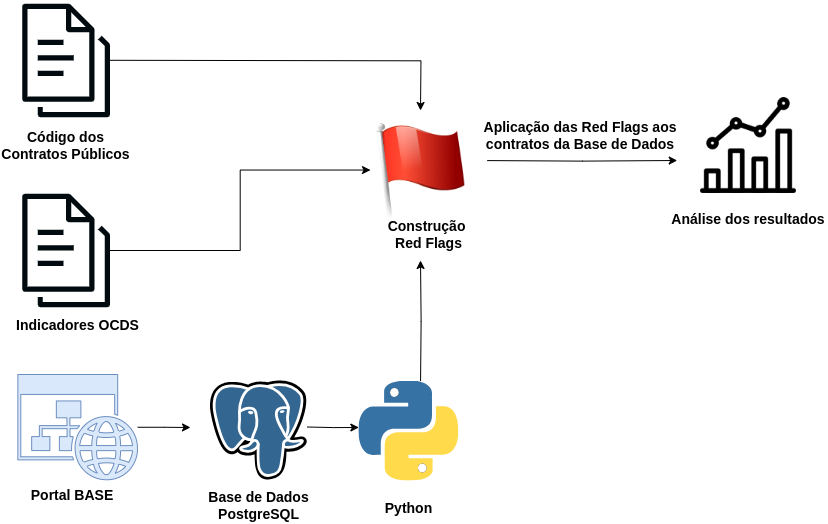
\includegraphics[width=0.85\textwidth]{imagens/processo_tese.png}
	\caption{Ilustração do conjunto de etapas envolvidas na elaboração do presente projeto. }
	\label{fig:processo}
\end{figure}

Ao longo deste texto, para todos os números referentes a valores pecuniários dos itens apresentados, o separador decimal será representado por vírgula e o separador dos milhares por ponto. Assim, o valor $20.315,42$ € corresponde a vinte mil, trezentos e quinze euros e quarenta e dois cêntimos. 

O desenvolvimento em software foi feito recorrendo à linguagem de programação Python (versão 3.11.8), ao sistema gerenciador de base de dados PostgreSQL (versão 8.1), à plataforma de controlo de versão Github, ao sistema de \textit{containerization} Docker (versão 25.0.3) e ao serviço de \textit{cloud} AWS. 


























































\section{Organização da tese}

Este relatório é composto por sete capítulos e encontram-se organizados da seguinte forma: 

\begin{my_itemize}


	\item \textbf{Capítulo 1 - Introdução}. Nesta capítulo é definido o problema que se pretende resolver, qual a necessidade em resolvê-lo o procedimento e os moldes em que se executou. Por fim, é apresentada a organização do presente relatório. 
	
	
	\item \textbf{Capítulo 2 - Contratação Pública em Portugal}. Neste capítulo é feita uma apresentação do Código dos Contratos Públicos em Portugal, onde são apresentados os principais objetivos deste documento e definidos os procedimentos e constituintes da formação de um contrato público.

	
	\item \textbf{Capítulo 3 - Noções Matemáticas}. Neste capítulo são apresentadas ferramentas básicas de Estatística, utilizadas recorrentemente na análise de dados. É apresentada a noção geral de \textit{outlier} e uma alternativa de deteção para distribuições assimétricas.

	
	\item \textbf{Capítulo 4 - Base de Dados}. Este capítulo encontra-se dividido em duas partes. Na primeira parte é descrito o \textit{website} de onde são recolhidos os dados, como é que o mesmo se encontra estruturado e as entidades envolvidas na regulação do mesmo. Na segunda parte é descrita a base de dados, como funciona o processo de recolha de dados, quais as colunas que revelaram maior interesse ao longo do desenvolvimento do projeto e a organização dos dados consoante diferentes variáveis de interesse, tais como o tipo de procedimento, valor adjudicado, categoria do contrato e local de execução.


	\item \textbf{Capítulo 5 - Aplicação de \textit{Red Flags}}. No início deste capítulo começa-se por apresentar o método de seleção de \textit{red flags}. De seguida, são caracterizadas as tabelas auxiliares da base de dados utilizadas ao longo do processo de construção das \textit{flags}. Por fim, é descrito o processo de construção de cada uma das flags desenvolvidas ao longo deste estágio e apresentados resultados após aplicação das mesmas.

	
	\item \textbf{Capítulo 6 - Processo de Automação}. Neste capítulo é descrito o processo de automação recorrendo à ferramenta de \textit{containerization} Docker e o serviço de \textit{cloud} AWS.

	
	\item \textbf{Capítulo 7 - Conclusão}. Por fim, neste capítulo, são sumariadas principais conclusões retiradas finda a construção e aplicação das \textit{red flags}, bem como possíveis melhorias e desenvolvimentos a serem considerados futuramente. 


\end{my_itemize}








\chapter{Fraude e Corrupção na Contratação Pública}
\input{chapters/fraude.tex}



\chapter{Contratação Pública em Portugal}
%A Contratação Pública em Portugal pode ser classificada de duas formas: aberta e fechada. As regras presentes no Código dos Contratos Públicos (CCP) dizem respeito aos contratos públicos celebrados entre uma entidade adjudicante pública e uma entidade adjudicatária.

%sendo esta composta por atos e formalidades relativos à formação, conclusão e produção de uma plena eficácia jurídica de um contrato público. A eficácia jurídica - ao contrário da eficácia social - é um conceito teórico, segundo o qual uma norma definida de acordo com a lei se torna eficaz em termos jurídicos. \\

%O ato de adjudicar consiste em conferir o direito de algo a alguém, conceder algo ao maior licitante ou atribuir algo a alguém por concurso ou por ajuste. 
%Este é um termo essencial na área de contratação pública, sendo esta constituída pelas entidades adjudicantes e entidades adjudicatárias. 

%O CCP é aplicado a entidades adjudicantes públicas, tais como o Estado, Regiões Autónomas, Autarquias locais, Institutos públicos, Entidades Administrativas Independentes, Banco de Portugal, Fundações Públicas, Associações Públicas, Associações de que façam parte uma ou várias pessoas coletivas referidas anteriormente e que sejam maioritariamente financiadas por estas. Além destas, são consideradas entidades adjudicantes organismos de direito público, pessoas coletivas e associações \footnote{nos termos do artigo 2.º n.º 2, alíneas a), b) e d)}. São consideradas, também, entidades adjudicantes organismos com atuação nos setores especiais da água, energia, tranposrtes e serviços postais \footnote{artigo 7.º n.º 1.º}. Existe, também, a possibilidade de aplicar o CCP a entidades não adjudicantes que pretendem celebrar determinados contratos de empreitadas de obras públicas ou de serviços associados a obras \footnote{artigo 275.º}.


% Associações de que façam parte uma ou várias pessoas coletivas referidas anteriormente, desde que sejam maioritariamente financiadas por estas, estejam sujeitas ao seu controle de gestão ou tenham um órgão de administração, de direção ou de fiscalização cuja maioria dos titulares seja, direta ou indiretamente, designada pelas mesmas

% São ainda entidades adjudicantes organismos de direito público, pessoas coletivas e associações, independentemente da sua natureza pública ou privada, nos termos do artigo 2.º n.º 2, alíneas a), b) e d).

% Para além das entidades adjudicantes referidas no artigo 2º, são também entidades adjudicantes as referidas no artigo 7.º n.º 1.º, concretamente as pessoas coletivas que realizam atividades nos seguintes sectores especiais da água, energia, transportes e serviços postais.

% O CCP aplica-se ainda a entidades que não sendo adjudicantes, se encontrem nas situações previstas no artigo 275.º, ou seja, entidades que pretendam celebrar determinados contratos de empreitadas de obras públicas ou de serviços associados a obras, desde que estes contratos sejam subsidiados diretamente em mais de 50\% do respetivo preço contratual por entidades adjudicantes, sempre que o preço contratual for igual ou superior aos limiares comunitários.


%Existem duas fases principais no processo de contratação pública. 
%A primeira fase é a \textbf{fase preparatória} em que é feita a decisão de realizar um contrato e inclui uma fase preparatória do procedimento e uma fase instrutória que terminará no ato de ajudicação. A segunda fase é a \textbf{fase conclusiva} em que é concluído e celebrado o contrato. Existe também uma \textbf{fase complementar} que pode ser necessária na eventualidade do contrato público depender de atos posterioes à sua celebração tais como a aprovação, visto e publicidade. \\

\section{Código dos Contratos Públicos}

O Código dos Contratos Públicos (CCP) é um documento que estabelece um alinhamento com as mais recentes diretivas comunitárias,  estabelecidas pelo Parlamento Europeu \cite{ue_dire}, definindo um conjunto homogéneo de normas relativas aos processos pré-contratuais e uma nova sistematização e uniformização de regimes substantivos dos contratos administrativos. 

Este encontra-se dividido em duas grandes categorias: \textbf{disciplina aplicável à contratação pública} e \textbf{regime substantivo dos contratos públicos}, correspondentes às Partes II e III do documento, respetivamente.

O CCP pauta-se por um conjunto de objetivos gerais que podem ser observados na figura \ref{fig:ccpgoals}.

\begin{figure}[H]
	\centering
	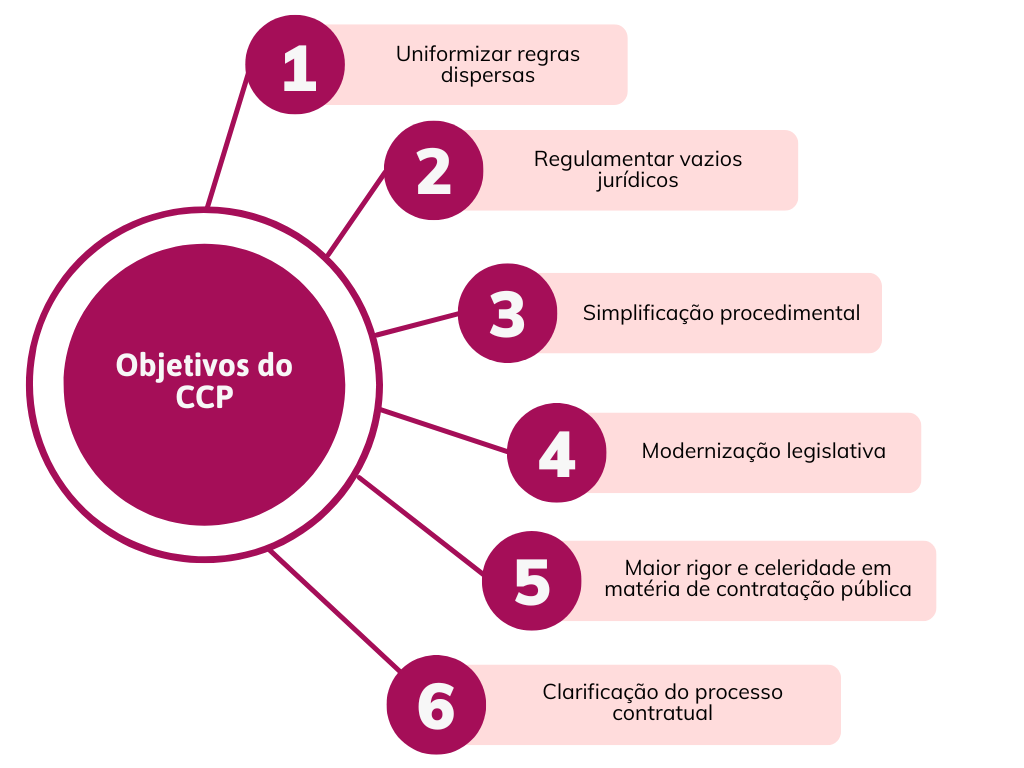
\includegraphics[width=0.7\textwidth]{imagens/ccp_objetivos.png}
	\caption{Objetivos Gerais do Código dos Contratos Públicos}
	\label{fig:ccpgoals}
\end{figure}


Pretende-se simplificar a tramitação procedimental pré-contratual através de novas tecnologias de informação/meios eletrónicos, incentivando a desburocratização, a desmaterialização, criando sistemas alternativos à utilização de papel, e a simplificação da contratação pública. 


Ao longo do processo contratual são definidas vários requisitos que devem ser cumpridos.
Relativamente ao \textbf{nível de qualificação dos candidatos}, é exigido que os mesmos demonstrem que possuem tanto capacidade técnica como financeira a fim de completar o objeto contratual. 

É imperativo que os \textbf{métodos de avalição de propostas}, componente crucial na formação e celebração de contratos públicos, sejam devidamente enunciados e publicitados, de modo a que as entidades concorrentes desenvolvam uma estratégia/proposta eficiente e a entidade adjudicante escolha, à luz desses mesmos critérios, a proposta mais vantajosa a nível económico na ótica do interesse prosseguido. 

Além do mais, o CCP procura, de forma cabal, garantir que a enunciação e publicitação dos critérios de adjudicação e respetivos coeficientes de ponderação se faça em moldes conformes com os princípos da igualdade, da concorrência, da imparcialidade, da proporcionalidade, da transparência, da publicidade e da boa fé. 




É, também, desejável que o objeto do contrato a celebrar \textbf{reflita e valorize preocupações de cariz social e ambiental}. 

O incumprimento da legislação pode levar a correções financeiras, cujas taxas são definidas em função da natureza e gravidade das irregularidades em causa e, consequentemente, a uma perda de financiamento. As irregularidades que são detetadas com maior frequência encontram-se disponíveis para consulta na Tabela COCOF \cite{corrections}.

\subsection{Entidades}

O artigo 2.º do CCP categoriza as entidades adjudicantes em dois organismos: Organismos pertencentes ao setor público administrativo tradicional e Organismos de direito público.


\begin{table}[h!]
	
	\centering
	\setlength{\tabcolsep}{15pt}
	\setlength\cellspacetoplimit{0.5cm} 
	\setlength\cellspacebottomlimit{0.5cm} 
	\renewcommand{\arraystretch}{1.5}

	\resizebox{\textwidth}{!}{
        \begin{tabular}{p{0.1\textwidth} p{0.1\textwidth} p{0.1\textwidth} p{0.25\textwidth} m{0.5\textwidth}} % Use p{} column type for vertical padding

			\hline
			\multicolumn{5}{Sc}{\textbf{Entidades Adjudicantes}} \\
			\hline
			\rowcolor[HTML]{EFEFEF} 
			\multicolumn{4}{Sc|}{\cellcolor[HTML]{EFEFEF}\textbf{Organismos pertencentes ao setor público administrativo tradicional}} & \textbf{Organismos de direito público} \\
			\hline
			Estado & Regiões Autónomas & Autarquias locais & Institutos públicos & \multirow{2}{=}{\centering Quaisquer pessoas coletivas que, independentemente da sua natureza pública ou privada, reúnam os requisitos presentes no n.º2 do artigo 2.º} \\ 
			Banco de Portugal & Fundações Públicas & Associações públicas & Entidades administrativas independentes & \\
			\hline
		\end{tabular}
	}
	
	\caption{Categorização das Entidades Adjudicantes}
	\label{table:1}
\end{table}



Existem, além das já mencionadas, outro tipo de entidades adjudicantes, também abrangidas pelo CCP, pertencentes aos setores especiais da água, energia, transportes e serviços postais. 

É de salientar que a denominação  de \textit{entidade adjudicante} apenas é válida durante a fase pré-contratual. Após a celebração do contrato, passa a ser denominada como \textit{contraente público}. 



\subsection{Procedimentos para formação de contratos}
%\subsubsection{Equadramento Legal}

\subsubsection{Tipos de Procedimento e Contrato}
Os procedimentos pré-contratuais definidos no n.º1 do artigo 16.º, a serem adotados pelas entidades adjudicantes, encontram-se na Tabela \ref{table:2}.

\begin{table}[ht]
	\centering
	\renewcommand{\arraystretch}{1.15}
	\setlength{\tabcolsep}{15pt}
	%\resizebox{\textwidth}{!}{%
		\begin{tabular}{lc}
			\toprule
			\multicolumn{1}{c}{\textbf{Tipo de Procedimento}} & \textbf{Artigo do CCP} \\ 
			\midrule
			\rowcolor[HTML]{EFEFEF} 
			Ajuste Direto                                     & 112.º a 129.º          \\ 
			Consulta Prévia                                   & 112.º a 127.º          \\
			\rowcolor[HTML]{EFEFEF} 
			Concurso Público                                  & 130.º a 161.º          \\
			Concurso Limitado por Prévia Qualificação         & 162.º a 192.º          \\
			\rowcolor[HTML]{EFEFEF} 
			Diálogo Concorrencial                             & 204.º a 218.º          \\
			Procedimento de Negociação                        & 193.º a 203.º          \\
			\rowcolor[HTML]{EFEFEF} 
			Parceria para a Inovação                          & 218.º-A a 218.º-D      \\
			Acordos-quadro                                    & 251.º a 259.º          \\                             
			\bottomrule
		\end{tabular}
	%}
	\caption{Tipos de Procedimento Pré-Contratuais}
	\label{table:2}
\end{table}


\begin{my_enumerate}
	
	\item O \textbf{ajuste direto} consiste no convite, por parte da entidade adjudicante, a um operador económico à sua escolha, a fim de apresentar uma proposta para um determinado objeto contratual.
	
	\item Na \textbf{consulta prévia}, a entidade adjudicante convida diretamente, pelo menos, 3 operadores económicos à sua escolha a apresentar uma proposta. Os aspetos referentes ao contrato a celebrar podem ser negociados diretamente entre a entidade adjudicante e os operadores convidados. 
	
	\item O \textbf{concurso público} pode ser adotado sempre que uma determinada entidade adjudicante o decidir. Não existe nenhuma fase prévia de qualificação dos concorrentes relativamente à capacidade técnico-financeira. 
	
	\item O \textbf{concurso limitado por prévia qualificação} é adotado quando o valor do contrato a celebrar for superior aos limiares Europeus. Neste caso, o concurso é dado a conhecer, não só através do Diário da República, como nos itens anteriores, como no Jornal Oficial da União Europeia. O \textbf{procedimento de negociação} partilha algumas características com este procedimento. 
	
	\item O \textbf{diálogo concorrencial} é utilizado nas situações em que a entidade adjudicante identifica uma necessidade e não sabe como satisfazer. 
	
	\item A \textbf{parceria para a inovação} destina-se à realização de atividades de investigação e desenvolvimente de bens, serviços ou obras inovadoras. Tem como objetivo a aquisição destes bens desde que se cumpram os níveis de desempenho de preços máximos
	previamente combinados. Acontece quando um entidade adjudicante pretende adquirir um bem/serviço/obra
	pública com determinadas características que não se encontram no mercado. 
	
	\item O \textbf{acordo quadro} é a celebração de um contrato entre uma ou várias entidades adjudicantes e uma ou mais entidades. 
	
	
	
\end{my_enumerate}

Em ambos os casos existem limitações relativamente aos operadores económicos que podem ser convidados. (artigos 19.o, al. d), e 20.o, n.o 1, al. d), 19.o, al. c), e 20.o, n.o 1, al. c)). Não obstante, as limitações referidas não se aplicam em contratos ao abrigo de critérios materiais. 
A celebração de consultas prévias e ajustes diretos deve ser publicitada no Portal dos Contratos Públicos pela entidade ajdudicante no prazo máximo de 20 dias a contar da data de celebração do contrato, a fim de comprovar a eficácia do respetivo contrato. 



%\textit{O CCP revê em alta ( o que é que isto significa? ) os limites relativos ao valor do contrato em função do procedimento pré-contratual adoptado. Para efeitos da determinação do valor do contrato, foi estabelecido que a escolha do procedimento condiciona o valor do contrato a celebrar. Por sua vez, o valor do contrato a celebrar pode ser entendido como o valor máximo do benefício económico obtido pelo adjudicatário com a execução de todas as prestações que constituem o objeto contratual.} \\



O n.º2 do mesmo artigo designa a tipologia do contrato a realizar, independentemente da sua natureza ou designação. 

\begin{table}[h!]
	\centering
	\renewcommand{\arraystretch}{1.15}
	\setlength{\tabcolsep}{15pt}
	%\resizebox{\textwidth}{!}{%
		\begin{tabular}{lc}
			\toprule
			\multicolumn{2}{c}{\textbf{Tipo de Contrato}}                                              \\ 
			\midrule
			Empreitada de obras públicas   &                                   \\
			Concessão de obras públicas                            & \multirow{-2}{*}{Obras}           \\ \hline
			Concessão de serviços públicos &                                   \\
			Locação ou aquisição de bens móveis                    &                                   \\
			Aquisição de serviços          &                                   \\
			Sociedade                                              & \multirow{-4}{*}{Bens e Serviços} \\ 
			\bottomrule
		\end{tabular}%
		%}
	\caption{Tipos de Contrato}
	\label{table:3}
\end{table}

FALAR DAS TIPOLOGIAS DE FORMA BREVE

\begin{figure}[H]
	\centering
	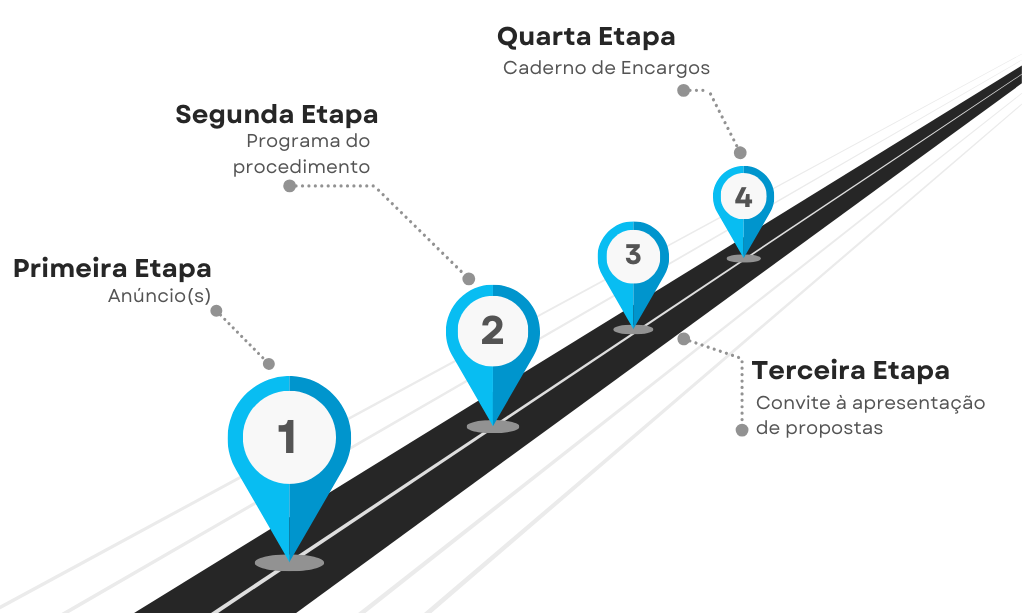
\includegraphics[width=0.75\textwidth]{imagens/pecasprocedimento.png}
	\caption{Peças do Procedimento}
	\label{fig:pecas}
\end{figure}

Na figura \ref{fig:pecas} é possível visualizar, de uma forma simplista, as peças que são transversais a todos os tipos de procedimento. \footnote{No caso do Ajuste Direto e Consulta Prévia não são tidas em conta as duas primeiras etapas. No Diálogo Concorrencial existem outras etapas intermédias.} 
São estas peças que definem as formalidades e requisitos que devem cumpridos na fase de elaboração e apresentação de propostas pelas entidades concorrentes. 
O anúncio do concurso público é sempre feito no Diário da República e, sob determinadas circunstâncias, no Jornal Oficial da União Europeia. 
O programa do procedimento é o regulamento que define os termos que devem ser cumpridos desde a fase de formação do contrato até ao seu término \cite{programaproc}. 
Por sua vez, o caderno de encargos é a peça do procedimento onde estão definidas as cláusulas do contrato a celebrar \cite{caderno}. 


\subsubsection{Escolha do procedimento}

O artigo 36.º do CCP define que a escolha do tipo de procedimento aquando da decisão de contratar deve ser fundamentada. Antes da abertura de um procedimento de formação de contrato público, a entidade adjudicante pode efetuar consultas informais de mercado a serem, eventualmente, usadas no planeamento da contratação. No caso de essa consulta ser feita a uma empresa que, posteriormente, se candidate ao concurso em questão, deve ser comunicado essa informação aos restantes concorrentes e inclui-la nas peças do procedimento. 

Além do mais, aquando da escolha do tipo de procedimento, devem ser tidas em conta as duas possíveis modalidades: \textbf{Critério do Valor} e \textbf{Critério Material}. 
Se se optar pelo critério do valor, existem valores máximos tabelados para o valor que o contrato pode tomar, consoante o tipo de procedimento. Define-se como valor do contrato o valor máximo do benefício económico obtido pela entidade contratada após a completitude de todas as prestações pertencentes ao objeto contratual.


\begin{table}[h!]
	\centering
	\renewcommand{\arraystretch}{1.6}
	\setlength{\tabcolsep}{15pt}
	\resizebox{\textwidth}{!}{%
		\begin{tabular}{ccccc}
			\hline
			\multicolumn{2}{c}{\textbf{Tipo de Procedimento}}                     & \textbf{Preço Base}                        & \textbf{Objeto} & \textbf{Base Legal (CCP)} \\ \hline
			\multirow{5}{*}{Ajuste Direto} & \multirow{2}{*}{Regime Simplificado} & \textless{}= €10.000,00                    & Obras           & artigo 128.º, n.º1        \\
			&                                      & \textless{}= €5.000,00                     & Bens e Serviços & artigo 128.º, n.º1        \\
			& \multirow{3}{*}{Regime Geral}        & \textless{}= €30.000,00                    & Obras           & artigo 19.º, al d)        \\
			&                                      & \textless{}= €20.000,00                    & Bens e Serviços & artigo 20.º, n.º1, al c)  \\
			&                                      & \textless{}= €50.000                       & Outros          & artigo 21.º, n.º1, al c)  \\ \hline
			\multicolumn{2}{c}{\multirow{3}{*}{Consulta Prévia}}                  & \textless{}= €150.000,00                   & Obras           & artigo 19.º, al c)        \\
			\multicolumn{2}{c}{}                                                  & \textless{}= €75.000,00                    & Bens e Serviços & artigo 20.º, n.º1, al c)  \\
			\multicolumn{2}{c}{}                                                  & \textless{}= €100.000                      & Outros          & artigo 21.º, n.º1, al c)  \\ \hline
			\multicolumn{2}{c}{\multirow{3}{*}{Concurso Público}}                 & \multirow{2}{*}{Até aos Limiares Europeus} & Obras           & artigo 19.º, al b)        \\
			\multicolumn{2}{c}{}                                                  &                                            & Bens e Serviços & artigo 20.º, n.º1, al b)  \\
			\multicolumn{2}{c}{}                                                  & Qualquer valor                             & Outros          & artigo 21.º, n.º1, al a)  \\ \hline
		\end{tabular}%
	}
	\caption{Valores máximos por tipo de procedimento}
	\label{tab:4}
\end{table}



Se for elegido o \textbf{Critério do Valor} é permitida a celebração de contratos de qualquer valor (de acordo com o artigo n.º23). Para tal, é necessário que o órgão competente para a decisão de contratar fundamente, de forma clara e objetiva, que a situação cumpre todos os requisitos previstos (nos artigos n.º24 a n.º27).


\subsubsection{Tipos de Contratos}

Os \textbf{contratos mistos} consistem num objeto contratual que contempla a prestação de dois ou mais tipos de contrato diferentes (nr.º1 do artigo 32.º). Por exemplo, o fornecimento de bens móveis e a prstação de serviços.

A \textbf{adjudicação por lotes} consiste na divisão de um contrato avultado em vários contratos de dimensão inferior, sendo o número máximo de lotes definido pela entidade adjudicante. Desta forma, é permitida a participação de pequenas e médias empresas que não teriam capacidade organizacional e técnico-financeira adequada para a realização total do contrato. 

\begin{table}[h!]
	\centering
	\renewcommand{\arraystretch}{1.45}
	\setlength{\tabcolsep}{15pt}
	\begin{tabular}{cc}
		\hline
		\textbf{Tipo de Contrato} & \textbf{Valor Mínimo} \\ \hline
		Bens e Serviços           & €135.000,00           \\
		Empreitadas               & €500.000,00           \\ \hline
	\end{tabular}
	\caption{Valor mínimo para Adjudicação por Lotes}
	\label{tab:5}
\end{table}

Contudo, em situações cujo preço do contrato a celebrar seja superior aos valores mínimos apresentados na tabela \ref{tab:5}, a adjudicação por lotes não é de cariz obrigatório. Carece, no entanto, de uma obrigação de fundamentação (nr.º2 do artigo 46.º-A). 


\subsection{Tramitação Procedimental}




\begin{figure}[H]
	\centering
	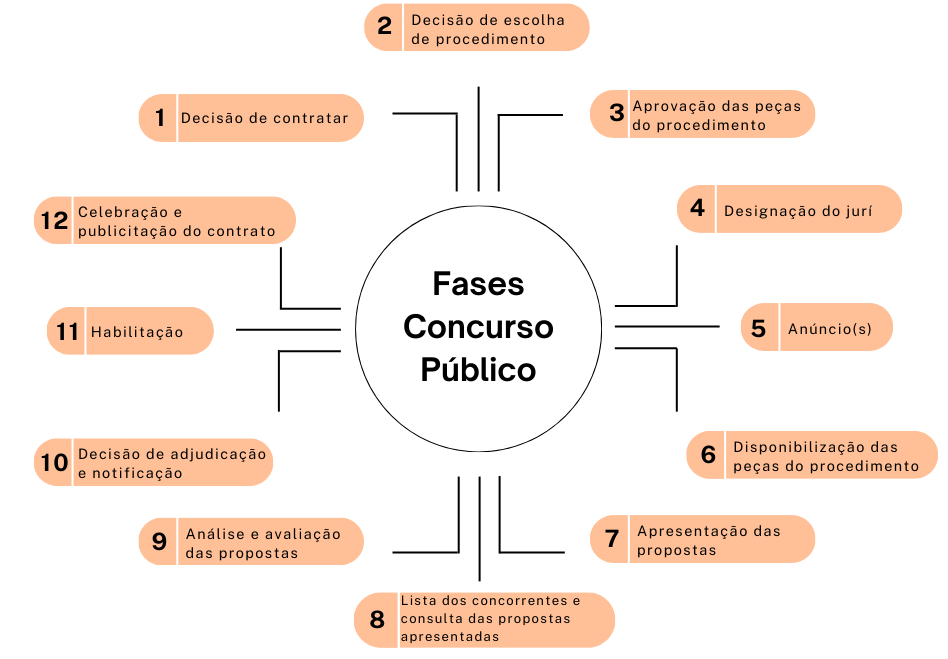
\includegraphics[width=\textwidth]{imagens/fasesconcpub.png}
	\caption{}
	\label{}
\end{figure}




%\chapter{Base de Dados}
%\section{Portal BASE}

O Portal BASE  é um \textit{website} que tem como missão a divulgação de informação relativa a contratos públicos celebrados em Portugal, ao abrigo do CCP.
Este espaço virtual, com a sua primeira versão lançada no ano de 2008, assume-se como a central de informação de contratação pública, onde são publicados os elementos referentes à formação e execução de contratos. 
Desta forma, é possível acompanhar e monitorizar os contratos, tornando o processo transparente e acessível a qualquer cidadão. 


%\begin{figure}[H]
%	\centering
%	
\includegraphics[scale=.5]{imagens/base.jpg}
%	\caption{Logotipo do Portal BASE}
%	\label{fig:base}
%\end{figure}



\subsection{Informação disponibilizada no Portal BASE}

No Portal BASE é possível encontrar informação relativa:

\begin{my_enumerate}
	\item Aos anúncios publicados no Diário da República relativos a procedimentos de formação de contratos públicos.
	\item Ao acesso às peças do procedimento.
	\item À formação dos contratos públicos sujeitos à parte II do CCP e à execução dos contratos administrativos sujeitos à parte III do CCP.
	\item À disponibilização e alienação de bens móveis.
	\item Às decisões definitivas de aplicação da sanção de proibição de participação previstas nos artigos 460.º e 464.º-A do CCP, durante o período da respetiva proibição.
	\item Às modificações objetivas de contratos que representem um valor acumulado superior a 10\% do preço contratual, as quais ficam disponibilizadas até seis meses após a extinção do contrato, nos termos do n.º 1 do artigo 315.º do CCP.
\end{my_enumerate}

Além do anteriormente mencionado, encontra-se disponível na Tabela \ref{tab:base} documentação suplementar relacionada com contratação pública.

%\begin{itemize}
%	\setlength{\itemsep}{0.2pt}
%	\setlength{\parskip}{-2pt}
%	\setlength{\parsep}{0pt}
%	
%	\item Legislação, regulamentação e jurisprudência nacional e comunitária
%	\item Guias de boas práticas e orientações técnicas
%	\item Informação estatística, na forma de relatórios anuais e sínteses mensais
%	\item Comunicados, notícias e eventos 
%
%\end{itemize}

\clearpage

\begin{table}[h!]
	\centering
	\resizebox{\textwidth}{!}{%
	\begin{tabular}{L L L L}
		\toprule
		Legislação, regulamentação e jurisprudência nacional e comunitária & Comunicados, notícias e eventos & Informação estatística, relatórios anuais e sínteses mensais & Guias de boas práticas e orientações técnicas \\
		\bottomrule
	\end{tabular}
	}
	\caption{Documentação suplementar disponível no Portal BASE}
	\label{tab:base}
\end{table}

A Figura \ref{fig:site1} reproduz a página inicial do \textit{website} do Portal BASE. Todas as entradas mencionadas na Tabela \ref{tab:base} podem ser facilmente consultadas na barra inicial delimitada a vermelho. É possível consultar, não só contratos, tal como se pode observar no rectângulo vermelho do lado esquerdo, assim como Anúncios, Entidades, Modificações Contratuais, Bens Móveis ou Impugnações. O campo \textbf{Pesquisa Avançada} permite selecionar vários parâmetros, nomeadamente, tipo de procedimento e contrato, intervalo de preço contratual, categoria de contrato, local de execução do contrato, data de celebração, entidade adjudicante e adjudicatária, entre outros. 

\begin{figure}[H]
	\centering
	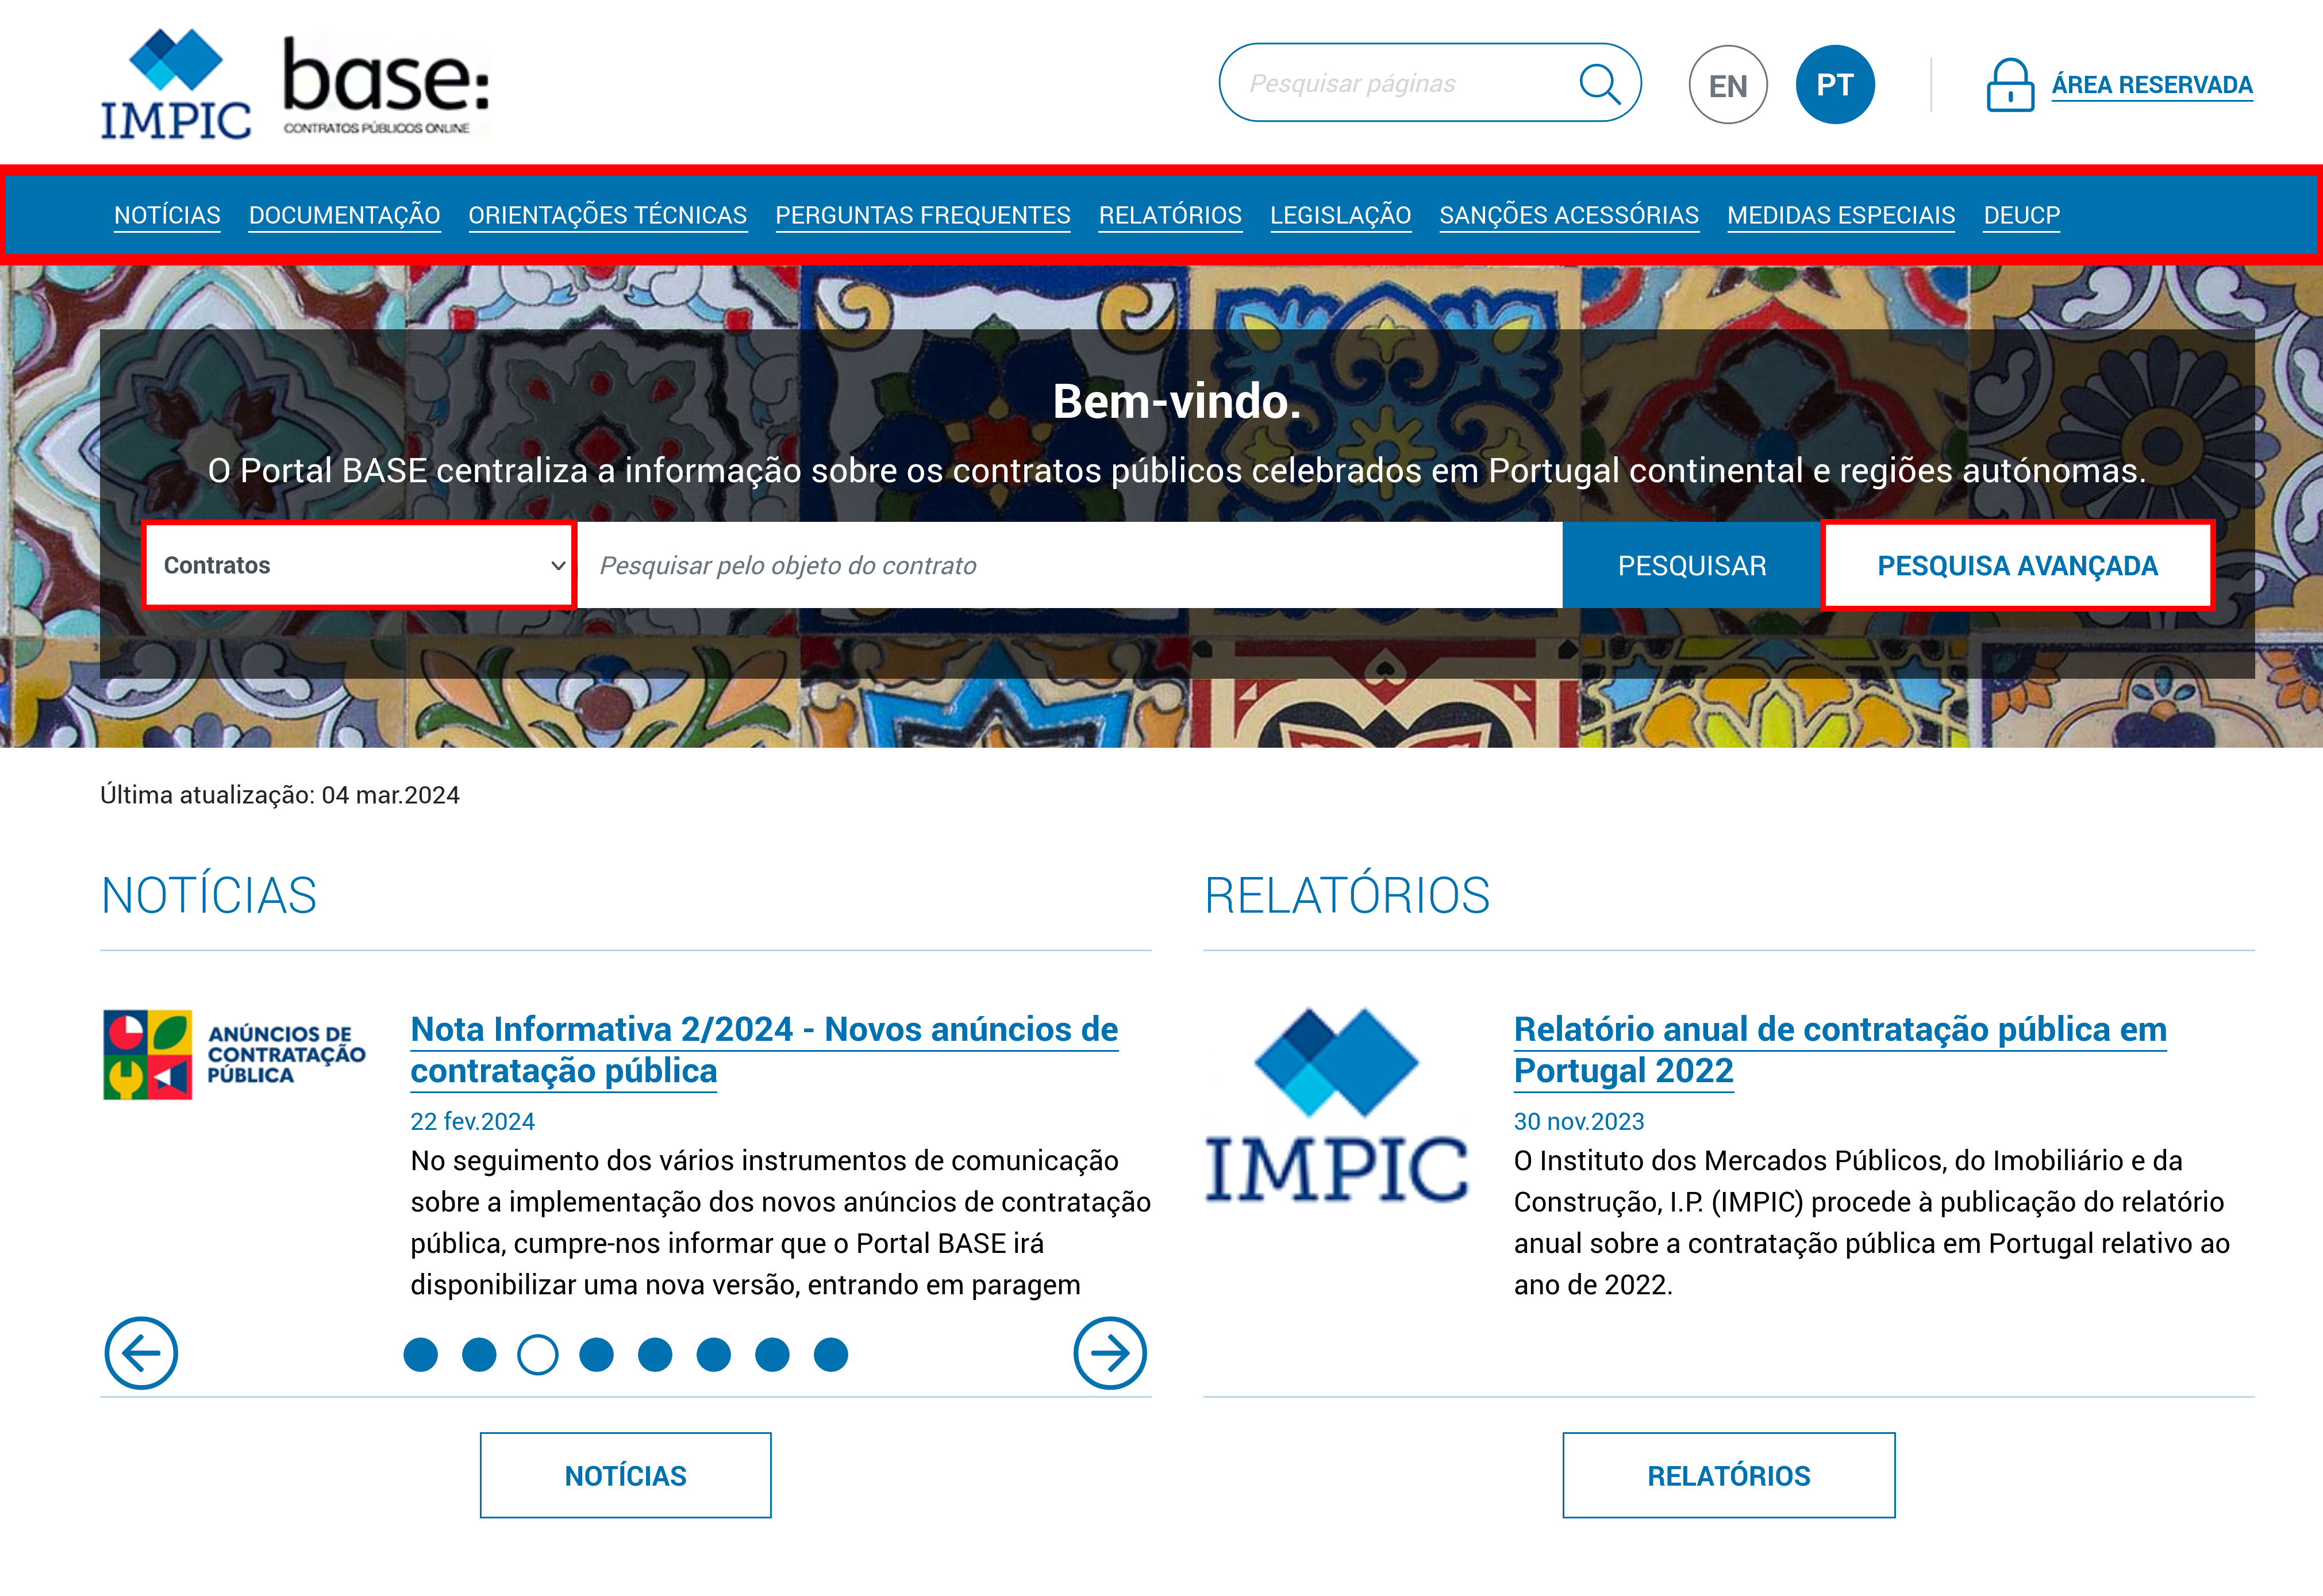
\includegraphics[width=\textwidth]{imagens/portalbase_init_v2.png}
	\caption{\textit{Screenshot} da página inicial do Portal BASE.}
	\label{fig:site1}
\end{figure}

\clearpage

\begin{figure}[H]
	\centering
	\includegraphics[width=\textwidth]{imagens/portalbase.png}
	\caption{\textit{Screenshot} do campo de pesquisa avançada do Portal BASE.}
	\label{fig:site2}
\end{figure}

Na Figura \ref{fig:site3} é possível verificar os últimos quatro contratos adicionados ao Portal BASE, no momento de captura de imagem do ecrã, dia 24 de abril de 2024. Para aceder às especificidades de cada um dos contratos é necessário pressionar o sinal \img{imagens/plus.png}, que se encontra delimitado a vermelho. A título de exemplo, identificam-se na Figura \ref{fig:site4} os detalhes contratuais do concurso público referente à contrução da nova linha de metro \textit{Rubi}, na cidade do Porto.

\begin{figure}[H]
	\centering
	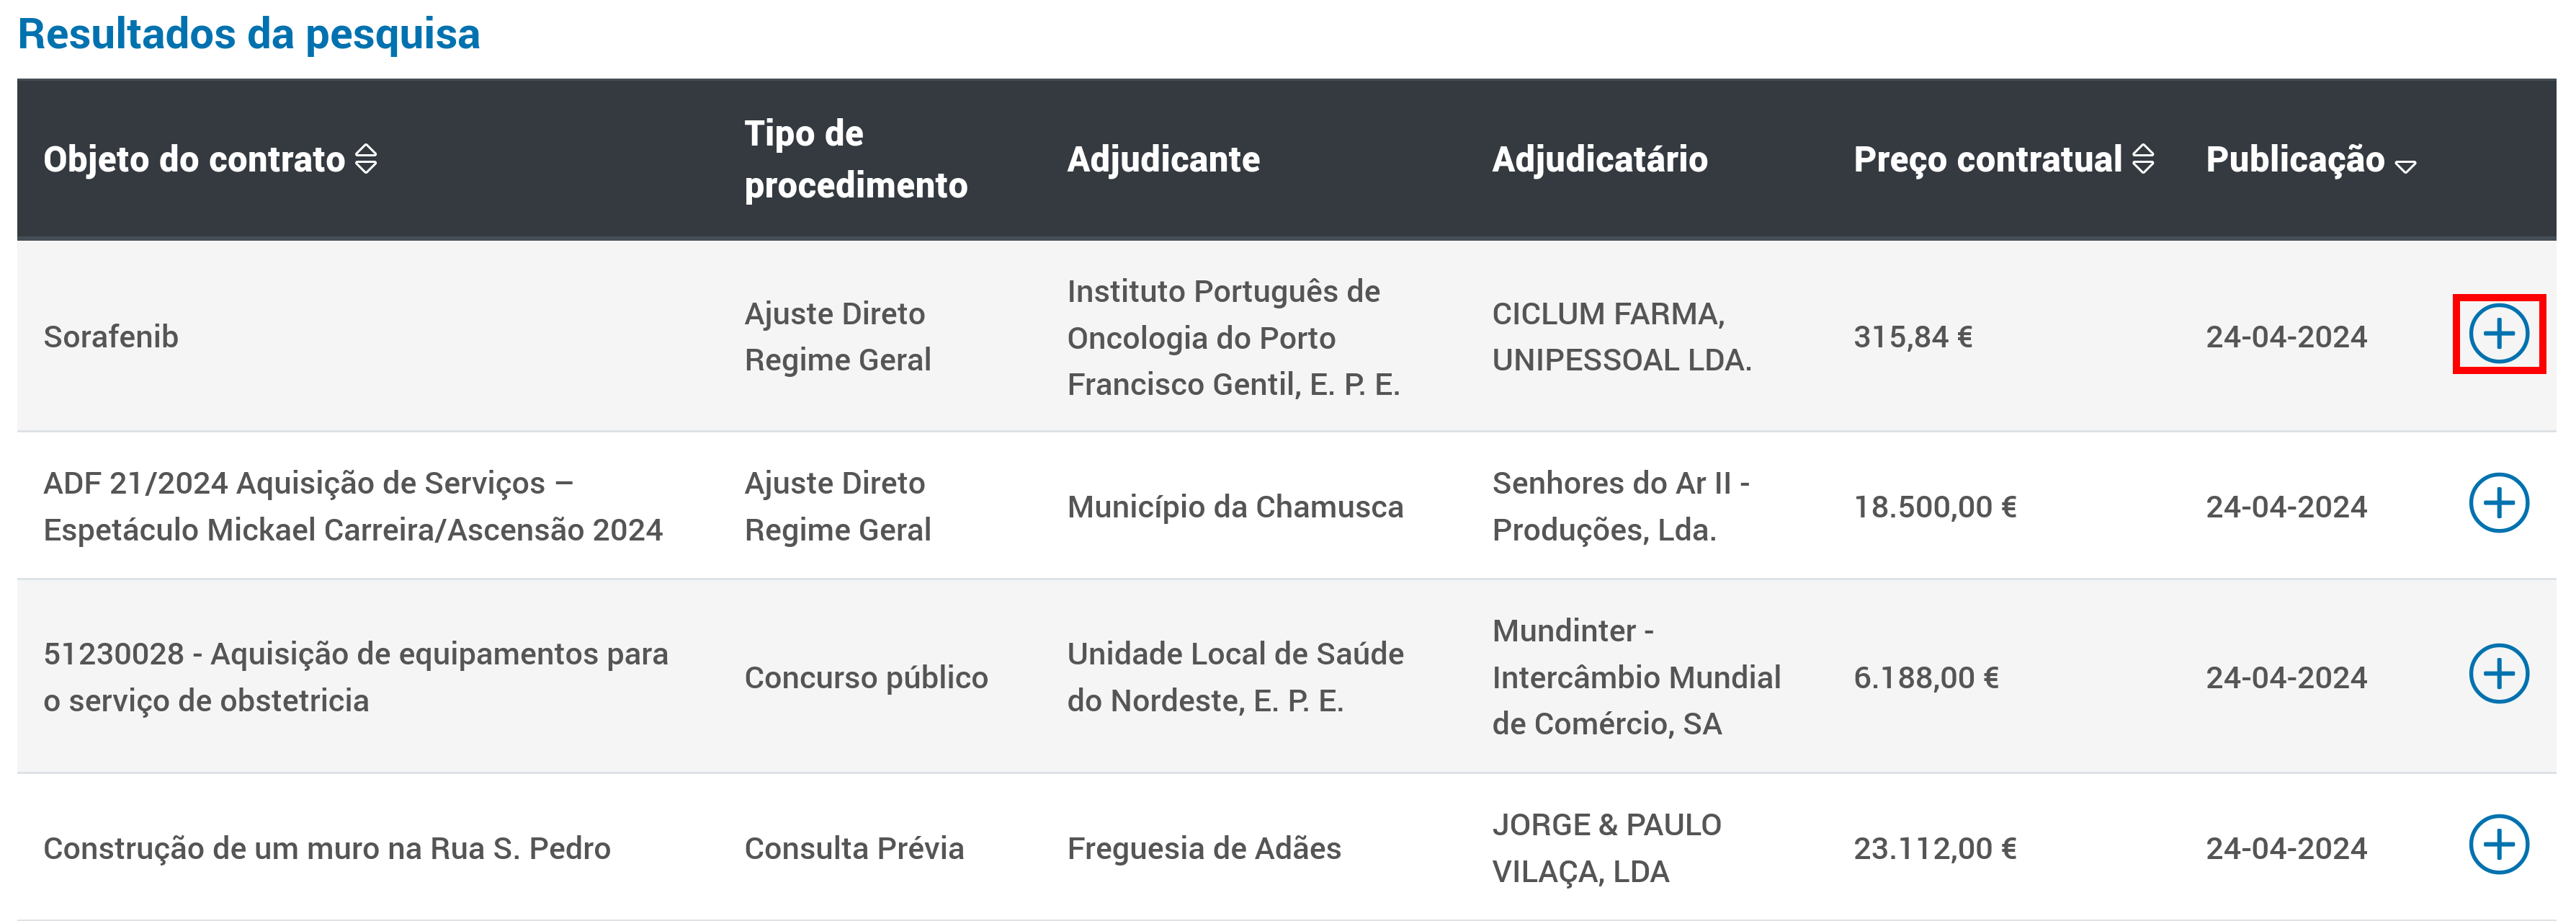
\includegraphics[width=\textwidth]{imagens/portalbase_pesquisa.png}
	\caption{\textit{Screenshot} dos últimos quatro contratos adicionados ao Portal BASE.}
	\label{fig:site3}
\end{figure}

\clearpage
\begin{figure}[H]
	\centering
	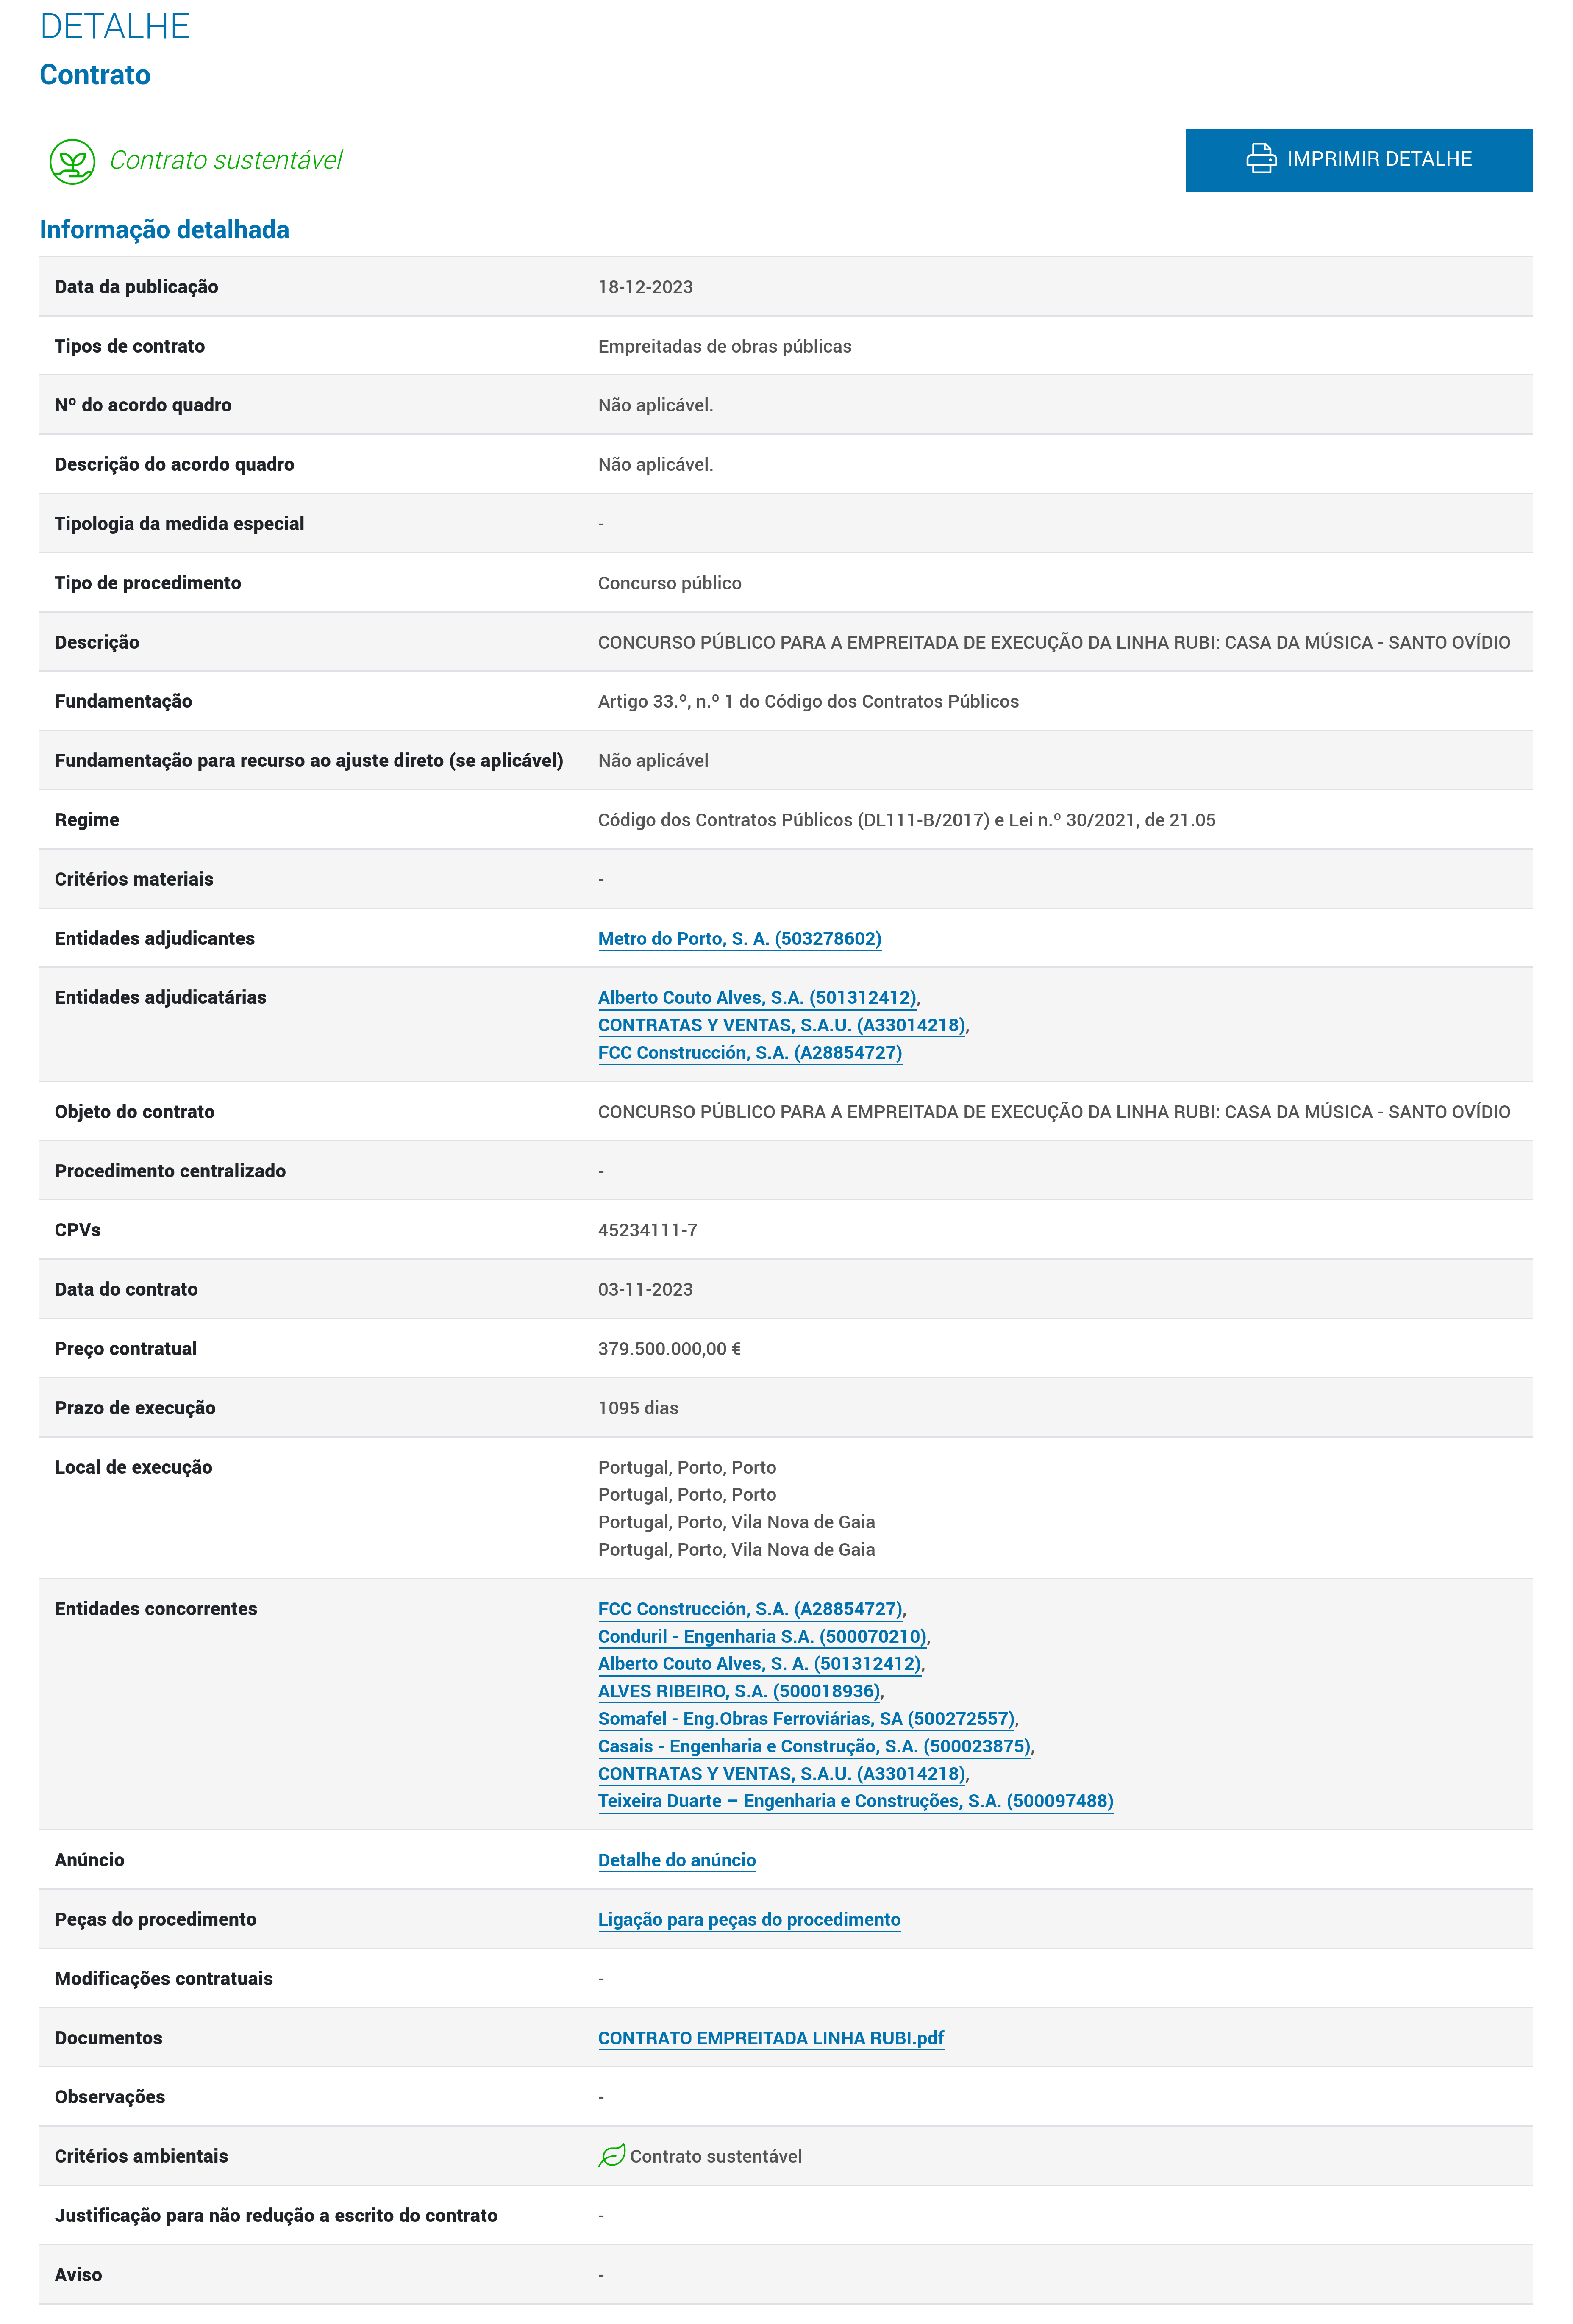
\includegraphics[width=\textwidth]{imagens/metro.png}
	\caption{\textit{Screenshot} dos detalhes do contrato referentes à contrução da Linha Rubi, do Metro do Porto.}
	\label{fig:site4}
\end{figure}

\clearpage
\subsection{Entidades envolvidas}

Existem diversas entidades que suportam o processo de contratação pública em Portugal. 

%\begin{figure}[h]
%	\centering
%	\begin{minipage}{.25\textwidth}
%		\centering
%		
\includegraphics[width=\linewidth]{imagens/ESPAP.png}
%	\end{minipage}%
%	\begin{minipage}{.25\textwidth}
%		\centering
%		
\includegraphics[scale = 0.1]{imagens/impic.jpg}
%	\end{minipage}%
%	\begin{minipage}{.25\textwidth}
%		\centering
%		
\includegraphics[width=\linewidth]{imagens/incm.png}
%	\end{minipage}%
%	\begin{minipage}{.25\textwidth}
%		\centering
%		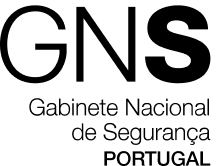
\includegraphics[width=.7\linewidth]{imagens/gns.png}
%	\end{minipage}
%	\caption{Entidades envolvidas no processo contratação pública}
%\end{figure}


\begin{my_enumerate}
	\item  \textbf{Instituto dos Mercados Públicos, do Imobiliário e da Construção, I.P. (IMPIC)}: É a entidade responsável por gerir o Portal BASE, monitorizar e fiscalizar as plataformas eletrónicas de contratação pública, regular os contratos públicos e assume-se como elo de ligação com a Comissão Europeia, para efeitos do disposto no nº 5, do artigo.º 83, da Diretiva nº 2014/24/EU. É responsável pelo desenvolvimento de manuais de boas práticas sobre contratos públicos de aquisição de obras, de bens e de prestação de serviços. Compete-lhe, ainda, a analise de queixas e denúncias de cidadãos e empresas.
	
	\item \textbf{Entidade de Serviços Partilhados da Administração Pública, I.P. (eSPap)}: É a entidade que desenvolve e presta serviços no âmbito da Administração Pública. Além disso, concebe, gere e avalia o sistema nacional de compras e assegura a gestão do Parque de Veículos do Estado (PVE), apoiando a definição de políticas estratégicas nas áreas das tecnologias de informação e comunicação (TIC), do Ministério das Finanças, garantindo o planeamento, conceção, execução e avaliação das iniciativas de informatização tecnológica dos respetivos serviços e organismos.
	
	\item \textbf{Gabinete Nacional de Segurança (GNS)}: É o organismo que garante a segurança da informação classificada de âmbito nacional e das organizações internacionais de que Portugal faz parte. É responsável por credenciar as plataformas eletrónicas de contratação pública, dos auditores de segurança, de pessoas e empresas para o acesso e manuseamento de informação classificada e entidades que atuem no âmbito do Sistema de Certificação Eletrónica do Estado - Infra-Estrutura de Chaves Públicas (SCEE).
	
	\item \textbf{Imprensa Nacional – Casa da Moeda (INCM)}: É a entidade responsável pelas publicações no Diário da República Eletrónico e no Jornal Oficial da União Europeia. Todos os anúncios dos procedimentos pré-contratuais (Concurso Público, Concurso Limitado por Prévia Qualificação, Procedimento de Negociação, Diálogo Concorrencial e Parceria para a Inovação) são publicados no Diário da República Eletrónico e, simultaneamente, publicitados no Portal BASE (excetuam-se os casos de ajuste direto e consulta prévia).
	
	\item \textbf{Entidades Adjudicantes}: São estas que conduzem e decidem o procedimento de formação de contrato e são responsáveis por introduzir, no Portal, informação sobre os contratos públicos celebrados. 
	
	\item \textbf{Adjudicatário}: Titular da proposta vencedora. Tem de comprovar que respeita os requisitos exigidos para poder celebrar o contrato. A informação é submetida no Portal BASE via plataforma eletrónica.
	
	\item \textbf{Plataforma Eletrónica}: É a infraestrutura tecnológica constituída por um conjunto de aplicações, meios e serviços informáticos onde, de forma totalmente eletrónica e desmaterializada, decorre a tramitação dos procedimentos para a formação de um contrato público. 
	
\end{my_enumerate}







\section{Descrição da Base de Dados}
\label{ch:variables}


O conjunto de dados contratuais disponibilizado e utilizado ao longo deste projeto encontra-se armazenado numa base de dados, em PostgreSQL. Salvo raras exceções, são adicionados ao Portal BASE, com caráter diário, os mais recentes contratos celebrados. Além disso, diariamente, são adicionados à base de dados todos os novos contratos do dia anterior, havendo, por isso, um desfasamento de um dia de forma a garantir que todos eles são coletados. 


\begin{figure}[H]
	\centering
	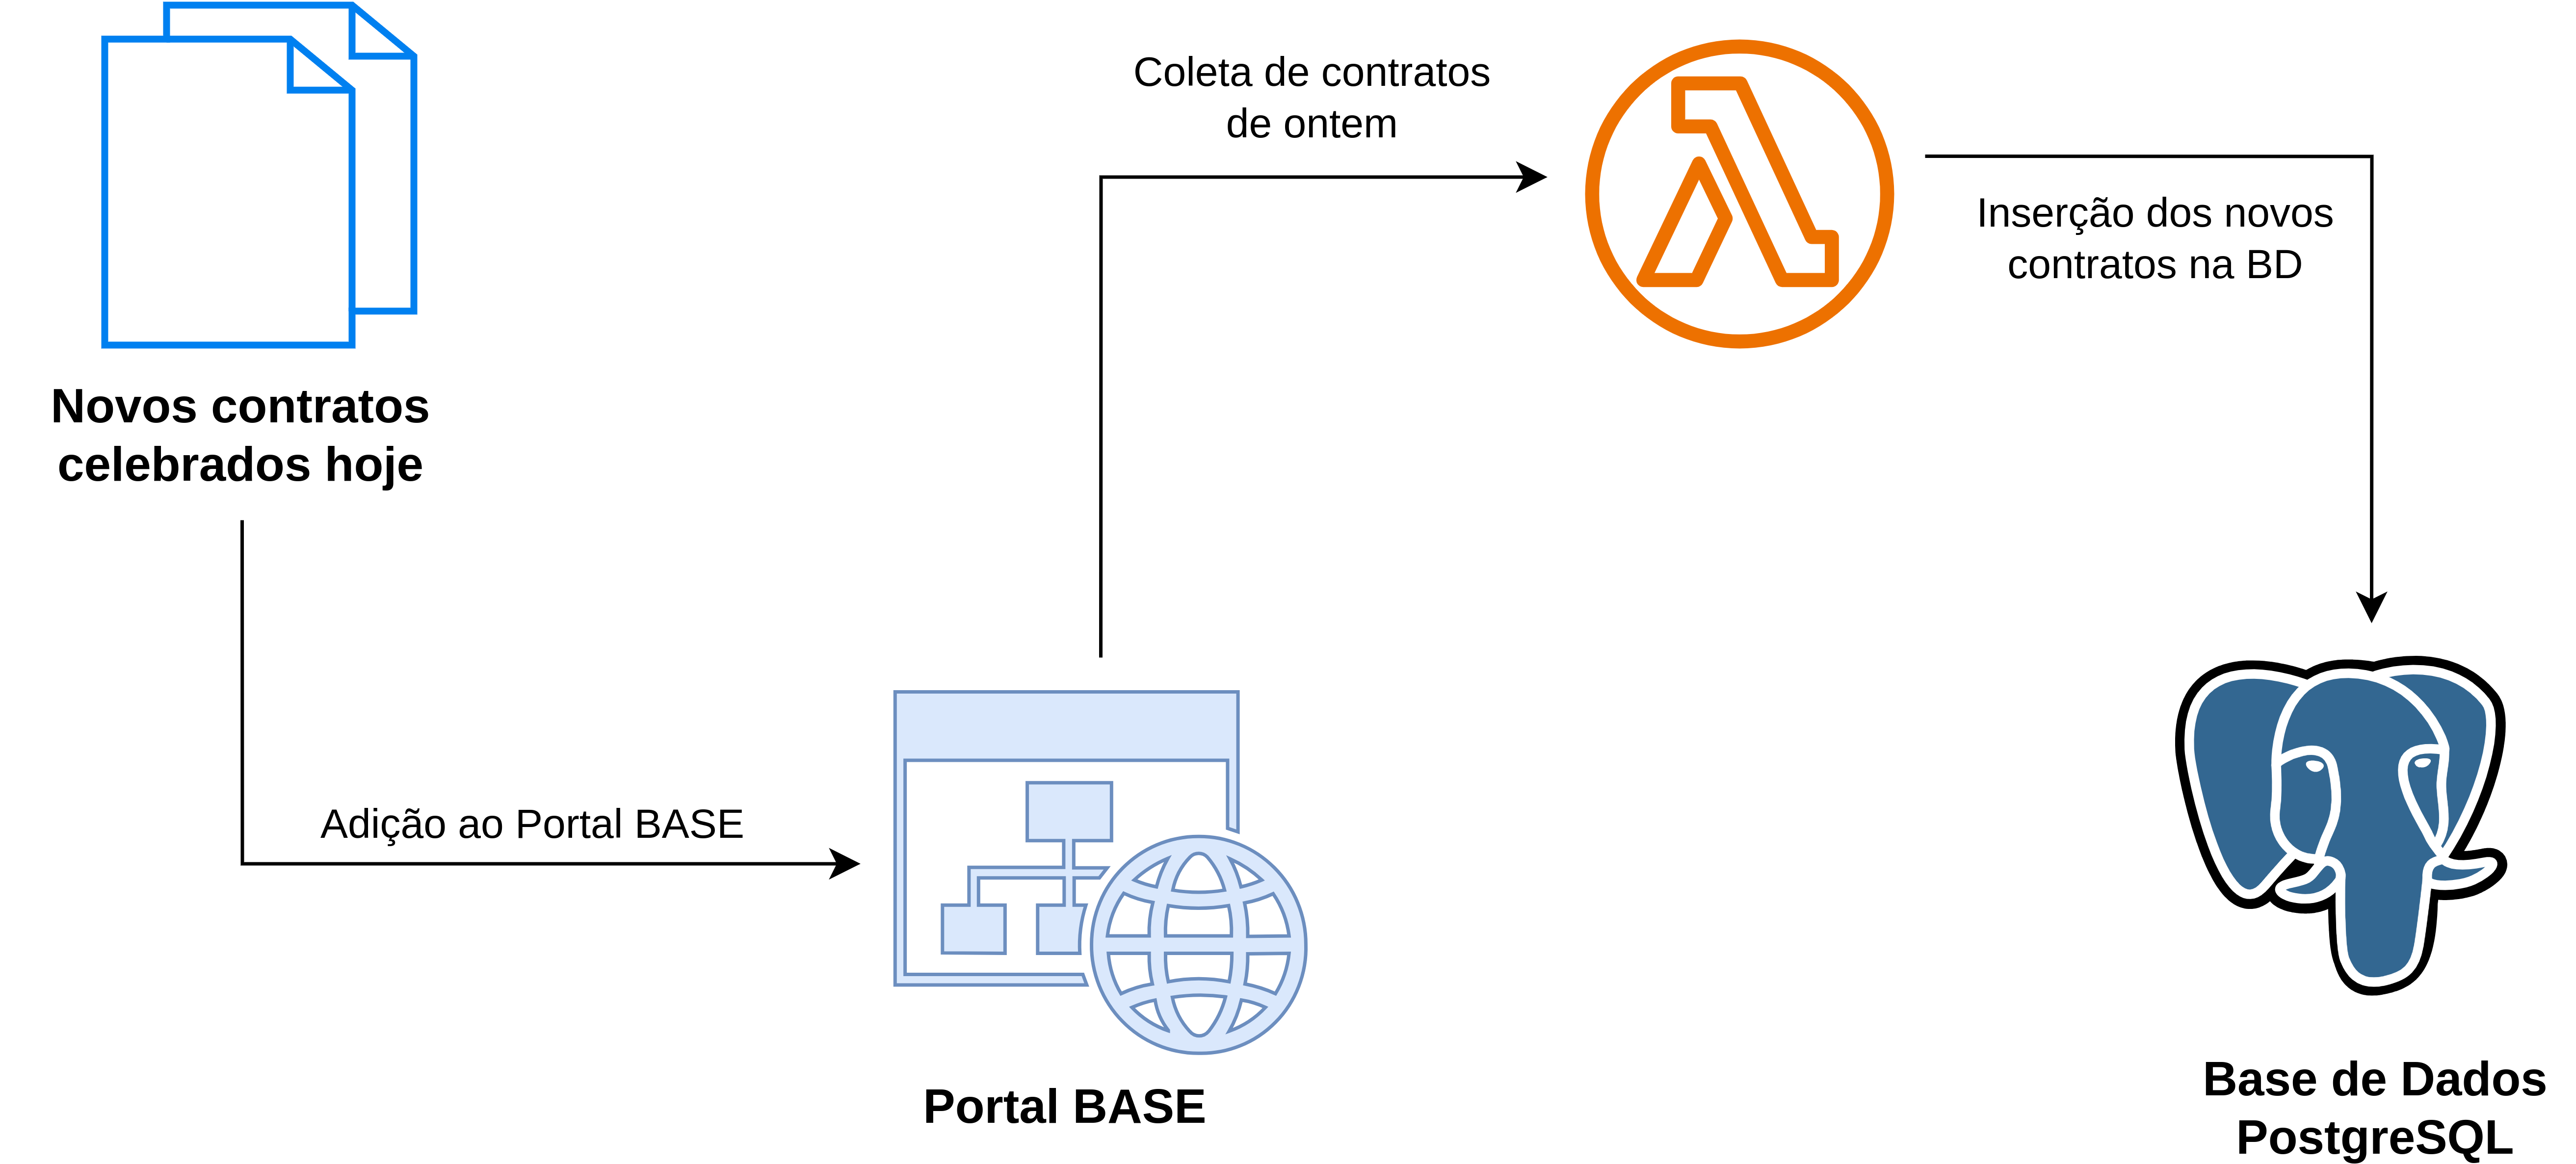
\includegraphics[width=0.7\textwidth]{imagens/portal_coleta.png}
	\caption{Processo de coleta de contratos e construção da base de dados.}
	\label{fig:processocoleta}
\end{figure}


Até ao primeiro dia do mês de maio, do presente ano civil, o conjunto de dados totalizava 1023443 contratos públicos, celebrados desde o dia 13 de maio de 2003. No trabalho que ora se apresenta, apenas foram considerados os contratos celebrados entre o dia 1 de janeiro de 2018 e o dia 1 de maio de 2024. Por assim ser, o número de contratos relativos ao ano de 2024 encontra-se incompleto. Pelo que, nas representações gráficas presentes nas secções que se seguem, a etiqueta relativa ao ano de 2024 será assinalada como \textbf{2024*}, a fim de sinalizar o facto de o conjunto não estar completo para o presente ano civil. 

Do total das 61 colunas da base de dados onde se encontram guardados todos os contratos públicos, as que revelaram maior interesse foram as seguintes: 


\begin{my_itemize}
	

\item \textbf{id} (integer): É o número que permite identificar um contrato específico na base de dados. A cada contrato foi atribuído um identificador único.


\item \textbf{n\_anuncio} (text): O número de anúncio é o número que permite identificar o anúncio no Diário da República Digital, referente a um determinado procedimento de contratação pública.


\item \textbf{anuncio\_preco\_base} (float): O preço base é definido como o preço máximo que a entidade adjudicante está disposta a pagar pela execução de todas as prestações que constituem o objeto do contrato a celebrar.


\item \textbf{anuncio\_proposalDeadline} (date): Este campo diz respeito ao número de dias estipulado para submeter uma proposta a um determinado concurso, por parte de uma entidade concorrente. 


\item \textbf{tipo\_procedimento} (text): Este parâmetro permite identificar o tipo de procedimento, de acordo com os enunciados na tabela \ref{table:2}, de um  determinado contrato público.


\item \textbf{objeto\_contrato} (text): O objeto de contrato consiste numa descrição detalhada do tipo de objeto celebrado. 


\item \textbf{data\_publicacao} (date): Este parâmetro diz respeito à data de publicação do contrato no Portal BASE.


\item \textbf{data\_celebracao} (date): Este parâmetro diz respeito à data de celebração do contrato. 

\item \textbf{preco\_contratual} (float): O  preço contratual é o preço a pagar pela entidade adjudicante à entidade vencedora após celebração do objeto contratual. 

\item \textbf{entidade\_adjudicante} (text): Este campo contém o nome, número de identificação fiscal e URL que remete para a página \textit{website} do Portal BASE com todos os contratos celebrados de uma determinada entidade adjudicante. 

\begin{figure}[H]
	\centering
	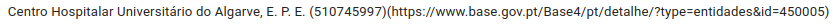
\includegraphics[width=.9\textwidth]{imagens/adjudicante.png}
	\caption{Exemplo de uma entidade adjudicante de um contrato presente na base de dados.}
	\label{fig:adjudicante}
\end{figure}

\item \textbf{fundamentacao} (text): A fundamentação diz respeito ao artigo do CCP utilizado para justificar a adoção do procedimento escolhido. 

\item \textbf{entidades\_contratadas} (text): À semelhança do campo \textbf{entidade\_adjudicante}, este campo contém o nome, número de identificação fiscal e URL que remete para a página \textit{web} do Portal BASE com todos os contratos celebrados de uma determinada entidade adjudicatária. 

\item \textbf{entidades\_concorrentes} (text): Neste campo é possível encontrar o nome, número de identificação fiscal e URL que remete para o \textit{website} do Portal BASE com todos os contratos celebrados para todas as entidades que concorrem a um determinado contrato público. Quando existe mais do que uma entidade concorrente, a separação entre entidades é feita através dos caracteres \(|||\).



\begin{figure}[H]
	\centering
	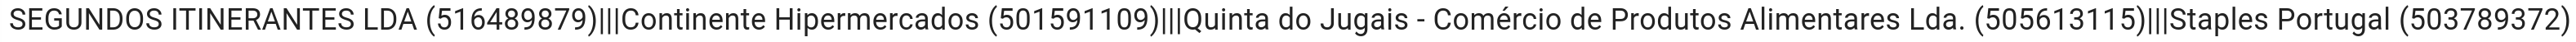
\includegraphics[width=.9\textwidth]{imagens/concorrentes.png}
	\caption{Exemplo de entidades concorrentes de um contrato presente na base de dados.}
	\label{fig:concorrentes}
\end{figure}


\item \textbf{url\_anuncio} (text): Contém um \textit{link} que redireciona para a página \textit{web} que contém os detalhes do anúncio.

\item \textbf{cpv} (text): Contém o CPV do contrato. CPV é a sigla de \textit{Common Procurement Vocabulary}. O CPV é um código de oito dígitos, usado no processo de contratação, que permite especificar e categorizar de forma hierárquica serviços e produtos. 

\begin{my_itemize}
	\item[$\circ$] \label{sec:cepeves}  Os 2 primeiros dígitos permitem identificar a \textbf{divisão} do serviço/produto. No total, existem 45 divisões.
	\item[$\circ$]  Os 3 primeiros dígitos permitem identificar o \textbf{grupo}. No total, existem 272 grupos.
	\item[$\circ$]  Os 4 primeiros dígitos permitem identificar a \textbf{classe}. No total, existem, 1002 classes.
	\item[$\circ$]  Os 5 primeiros dígitos permitem identificar a \textbf{categoria}. No total, existem 2379 categorias.
	\item[$\circ$]  Os 6 primeiros dígitos permitem identificar a \textbf{subcategoria}. No total, existem 5756 subcategorias.
\end{my_itemize}

A título de exemplo, atente-se no caso seguinte caso:

\begin{figure}[H]
	\centering
	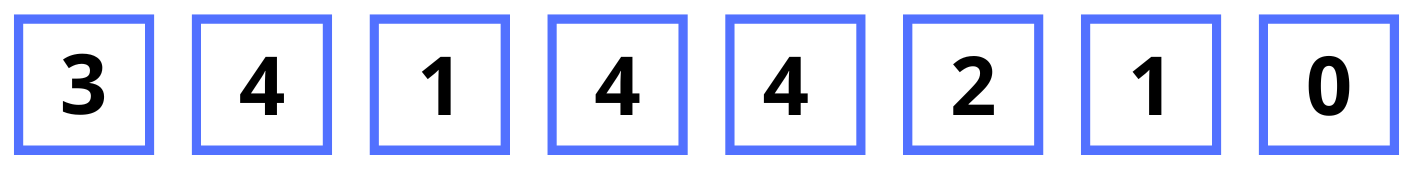
\includegraphics[width=0.7\textwidth]{imagens/cpv.png}
	\caption{Ilustração do CPV de um contrato referente a veículos de combate a incêndios.}
	\label{fig:cpv}
\end{figure}


\begin{my_itemize}
	\item[$\circ$]  \textbf{Divisão:} 34 - Equipamentos de transporte e produtos auxiliares ao transporte
	\item[$\circ$]  \textbf{Grupo:} 341 - Veículos motorizados
	\item[$\circ$]  \textbf{Classe:} 3414 - Veículos motorizados pesados
	\item[$\circ$]  \textbf{Categoria:} 34144 - Veículos motorizados para fins especiais
	\item[$\circ$]  \textbf{Subcategoria:} 34144210 - Veículos de combate a incêndios
\end{my_itemize}



\item \textbf{contractType} (text): Este campo diz respeito ao tipo de contrato celebrado, tal como se encontra apresentado Tabela \ref{table:3}. 

\item \textbf{executionPlace} (text): Indica o local de execução do contrato. 

\item \textbf{totalEffectivePrice} (float): Na eventualidade de existirem alterações do preço contratual após a celebração do contrato, este campo é preenchido. Existem, também, casos em que o preço contratual diz respeito à unidade em questão (p. ex. quilómetro, hora, dia). Nessa situação, o preço total efetivo é o preço total após prestação do serviço \cite{jardinagem}.  

\end{my_itemize}

De entre o universo de contratos celebrados, pode-se perceber na Tabela \ref{tab:contratos} como estes se distribuem consoante os diferentes tipos de procedimentos. Como se pode verificar, os tipos de procedimentos com maior relevância são: o Ajuste Direto em Regime Geral, a Consulta Prévia, o Concurso Público e contratos ao abrigo de acordo-quadro, com especial evidência para o Ajuste Direto em Regime Geral que prefaz 50\% dos contratos. 


\begin{table}[H]
	\centering
	\renewcommand{\arraystretch}{1.15}
	\setlength{\tabcolsep}{15pt}
	\resizebox{\textwidth}{!}} \\ \hline
			Ajuste Direto Regime Geral                                                     & 526860                                                                   & 51.4                                                            \\ \hline
			\rowcolor[HTML]{EFEFEF} 
			Consulta Prévia                                                                & 228400                                                                   & 22.3                                                            \\ \hline
			Concurso público                                                               & 128422                                                                   & 12.5                                                            \\ \hline
			\rowcolor[HTML]{EFEFEF} 
			Ao abrigo de acordo-quadro (art.º 259.º)                                       & 111723                                                                   & 10.9                                                            \\ \hline
			Ao abrigo de acordo-quadro (art.º 258.º)                                       & 24406                                                                    & 2.4                                                             \\ \hline
			Concurso limitado por prévia qualificação                                      & 1816                                                                     & $< 1$                                                            \\ \hline
			\rowcolor[HTML]{EFEFEF} 
			Consulta Prévia Simplificada                                                   & 958                                                                      & $< 1$                                                            \\ \hline
			Contratação excluída II                                                        & 485                                                                      & $< 1$                                                            \\ \hline
			Setores especiais – isenção parte II                                           & 222                                                                      & $< 1$                                                          \\ \hline
			\rowcolor[HTML]{EFEFEF} 
			Procedimento de negociação                                                     & 45                                                                       & $< 1$                                                          \\ \hline
			Concurso público simplificado                                                  & 42                                                                       & $< 1$                                                          \\ \hline
			\rowcolor[HTML]{EFEFEF} 
			Consulta prévia ao abrigo do artigo 7º da Lei n.º 30/2021, de 21.05            & 25                                                                       & $< 1$                                                          \\ \hline
			Ajuste Direto Regime Geral ao abrigo do artigo 7º da Lei n.º 30/2021, de 21.05 & 21                                                                       & $< 1$                                                          \\ \hline
			\rowcolor[HTML]{EFEFEF} 
			Serviços sociais e outros serviços específicos                                 & 9                                                                        & $< 1$                                                          \\ \hline
			Concurso de conceção simplificado                                              & 4                                                                        & $< 1$                                                          \\ \hline
		\end{tabular}%
	}
	\caption{Número de contratos públicos e respetiva fração para os vários tipos de procedimentos.}
	\label{tab:contratos}	
\end{table}



%\rowcolor[HTML]{EFEFEF} 
%Parceria para a inovação                                                       & 2                                                                        & $< 1$                                                          \\ \hline
%Concurso de ideias simplificado                                                & 1                                                                        & $< 1$                                                          \\ \hline
%\rowcolor[HTML]{EFEFEF} 
%Não especificado & 1                                                                        & $< 1$                                                           \\ \hline



A leitura das Figuras \ref{fig:numcontrs} e \ref{fig:precoscontrs} permite inferir uma tendência crescente do número de contratos celebrados entre 2018 e 2023, estando este comportamento em linha com o crescimento do preço contratual total por ano. 

\begin{figure}[H]
	\centering
	\begin{minipage}{.49\linewidth}
		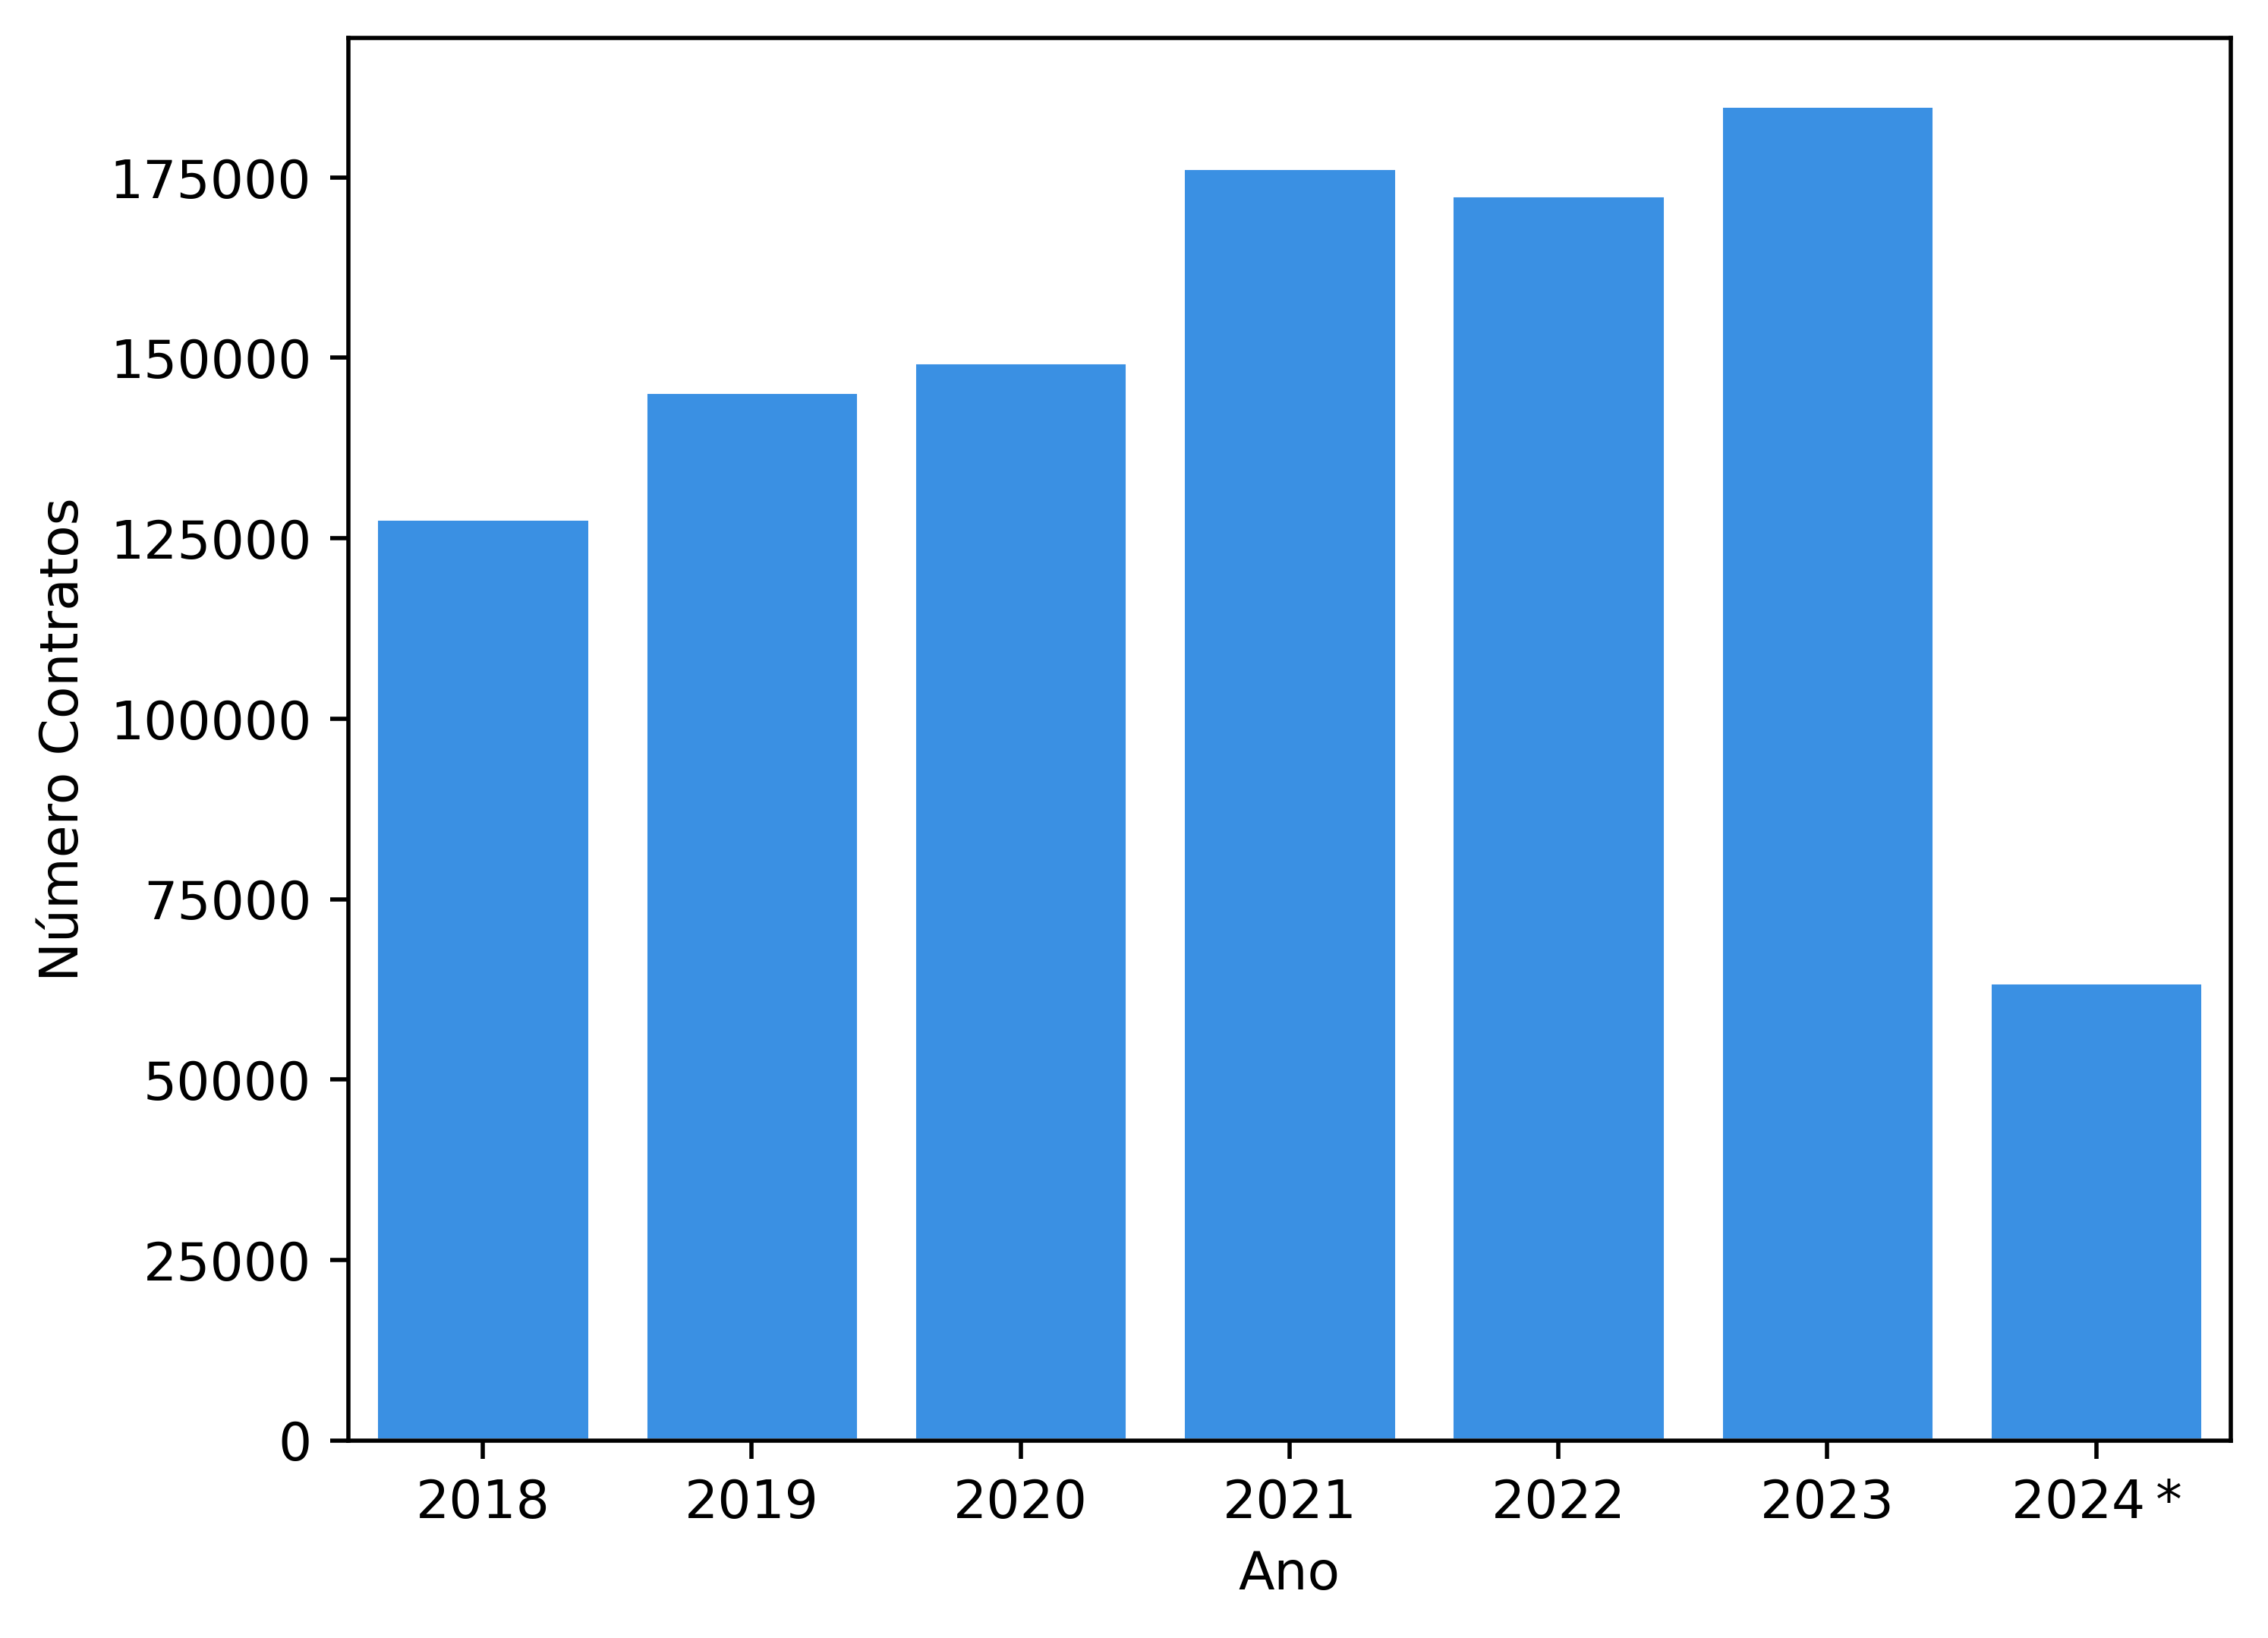
\includegraphics[width=\linewidth]{imagens/contratos_ano.png}
		\caption{Número de contratos celebrados, entre 2018 e 2024, para todas as tipologias.}
		\label{fig:numcontrs}
	\end{minipage}
	\hfill
	\begin{minipage}{.49\linewidth}
		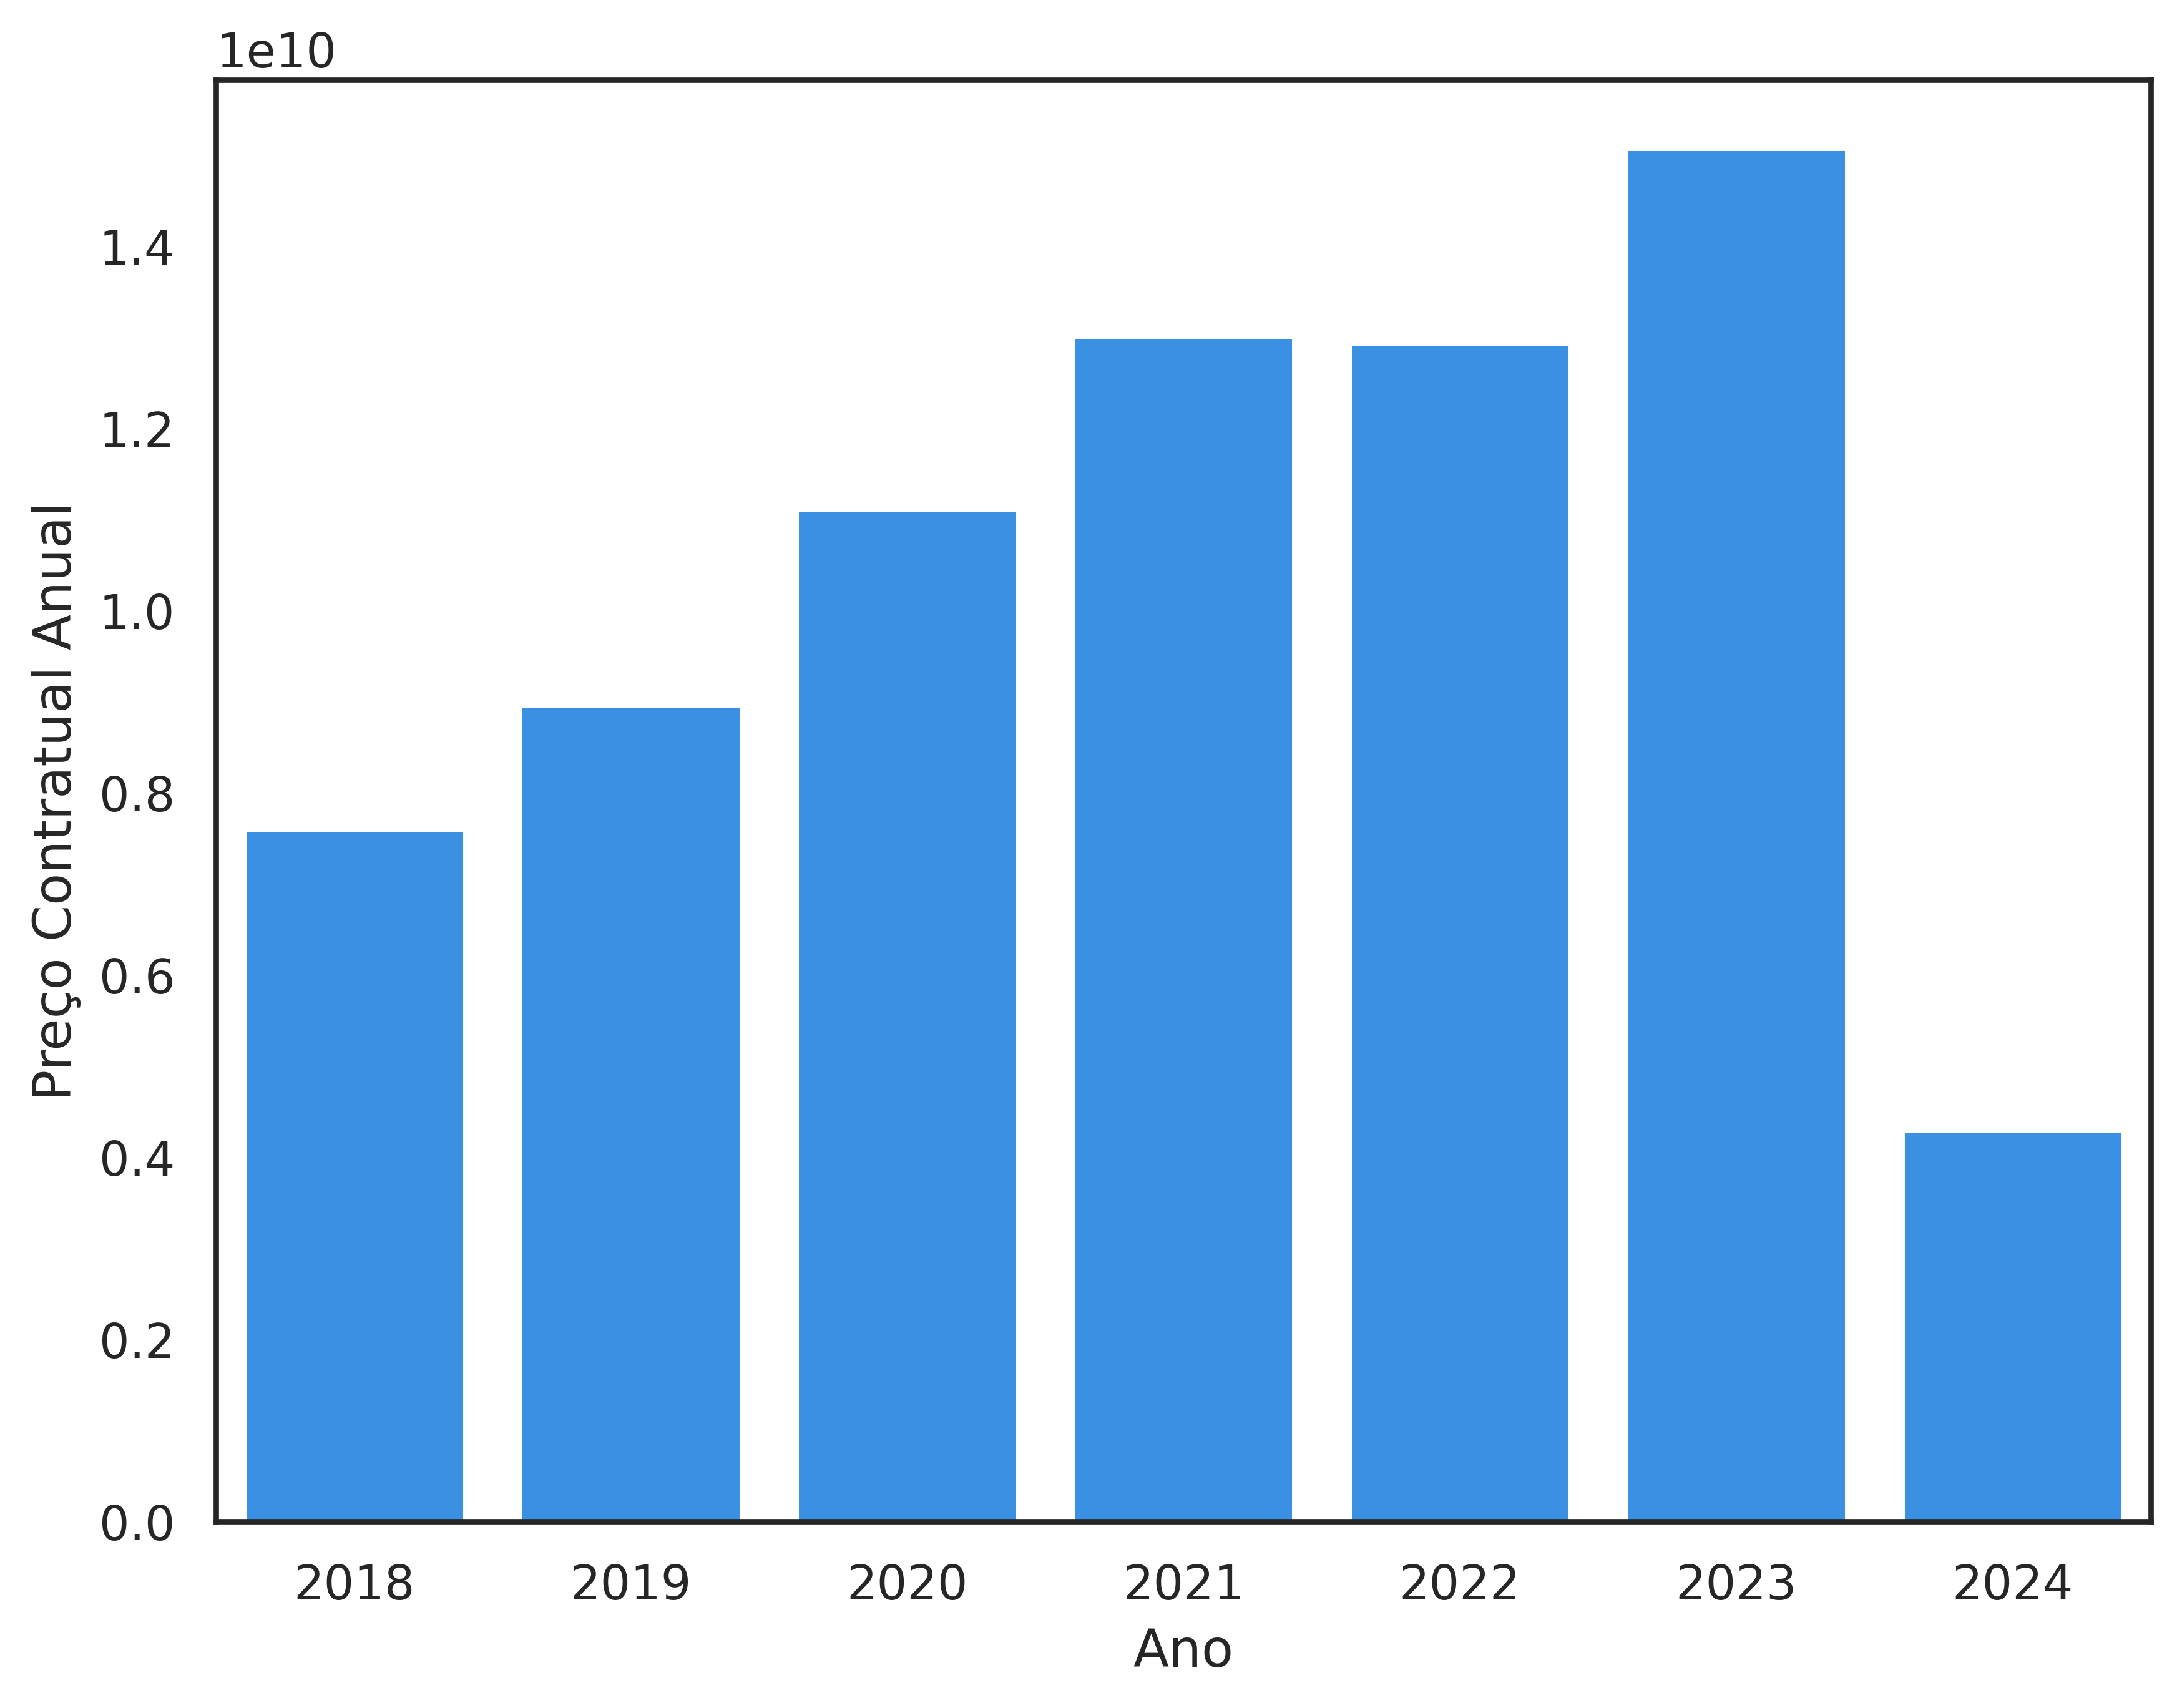
\includegraphics[width=\linewidth]{imagens/precocontr_ano.png}
		\caption{Preço contratual total, entre 2018 e 2024, para todas as tipologias}
		\label{fig:precoscontrs}
	\end{minipage}
\end{figure}


%\begin{wrapfigure}{R}{0.45\textwidth}
%	\centering
%	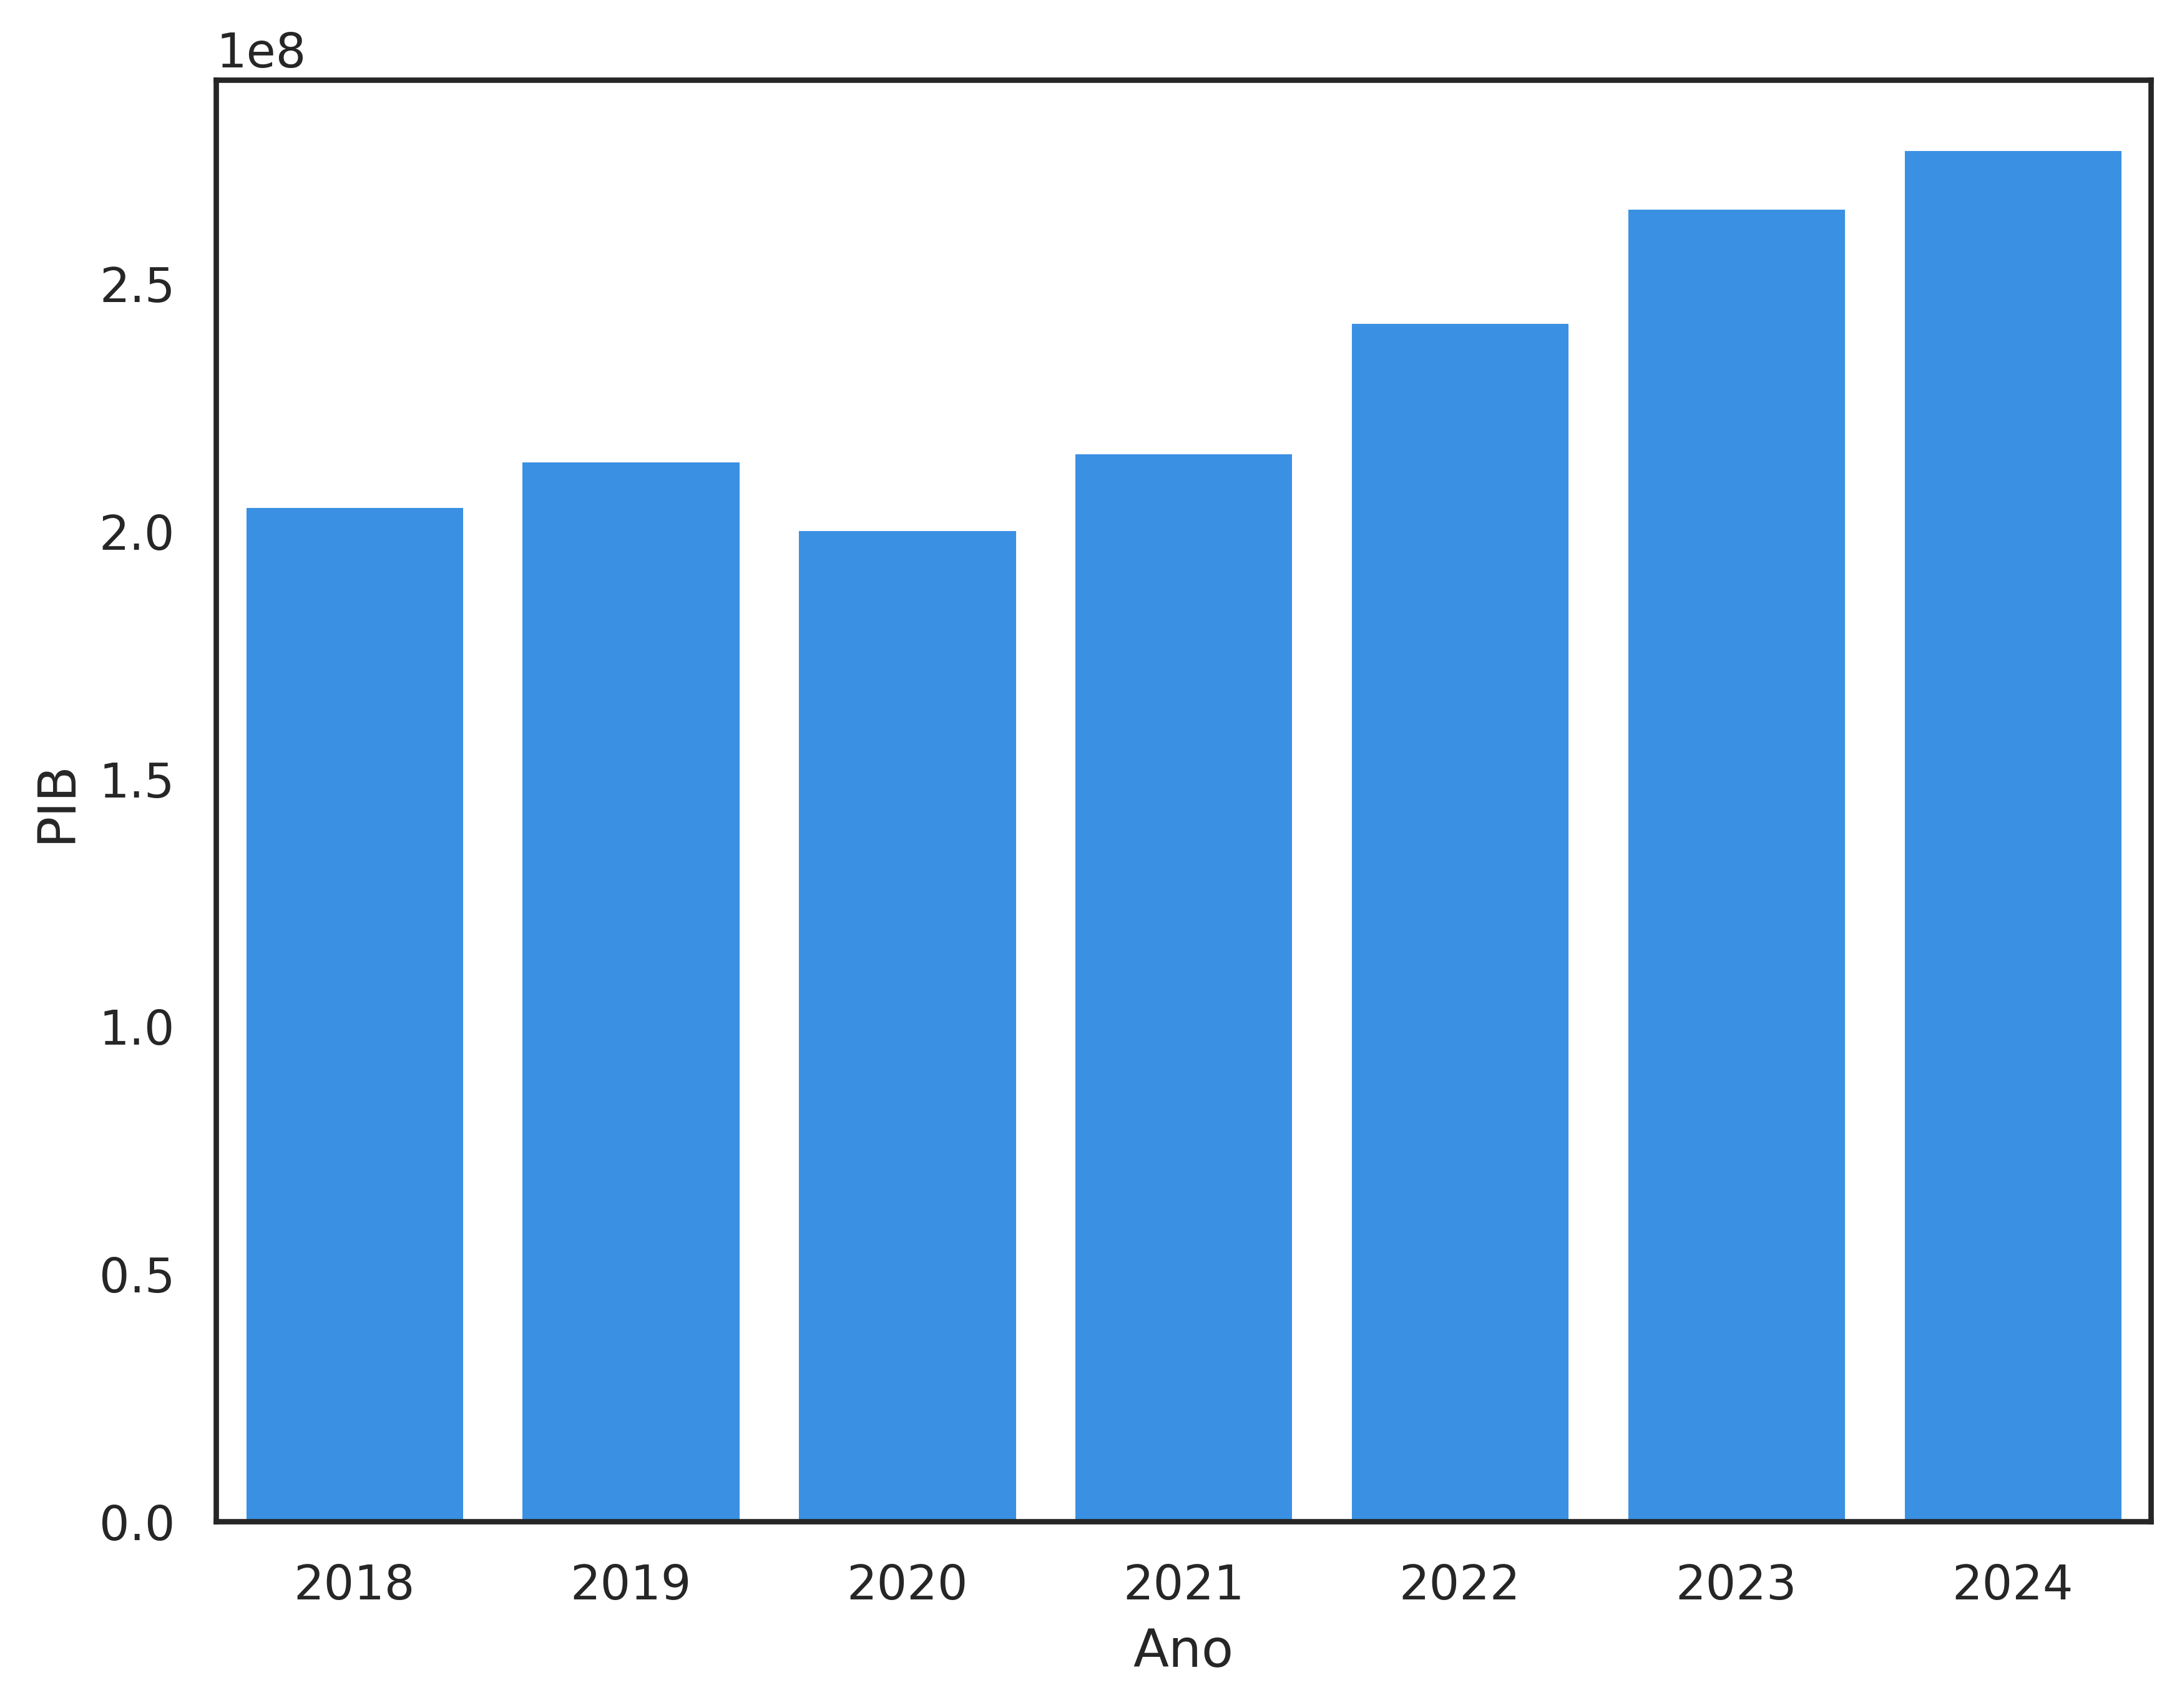
\includegraphics[width=0.45\textwidth]{imagens/pib.png}
%	\caption{PIB português entre 2018 e 2024}
%\end{wrapfigure}




\begin{table}[H]
	\centering
	\renewcommand{\arraystretch}{1.35}
	\setlength{\tabcolsep}{20pt}
	\resizebox{\textwidth}{!}{%
		\begin{tabular}{l|l}
			\textbf{33} & {\color[HTML]{000000} Equipamento médico, medicamentos, e produtos para cuidados pessoais}     \\
			\textbf{45} & Construção                                                                                     \\
			\textbf{79} & Serviços a empresas: direto, comercialização, consultoria, recrutamento, impressão e segurança \\
			\textbf{50} & Serviços de reparação e manuntenção                                                           
		\end{tabular}%
	}
	\caption{Descrição das principais divisões de CPV.}
	\label{tab:maincpvs}
\end{table}

Na Figura \ref{fig:distritos}, constata-se que existe uma prevalência de contratos celebrados nos distritos de Lisboa e do Porto, com 21\% e 14\%, respetivamente. Pelo contrário, considerando todos os distritos do interior, o valor aproxima-se dos 14\%. Existe, também, um elevado de número de contratos cujo distrito é identificado como \textit{Outro}. Estes casos, dizem respeito a erros de preenchimentos aquando da submissão dos contratos no Portal BASE, pois no campo \textbf{executionPlace} verificava-se um dos três cenários: o campo encontrava-se vazio, era inserido \textit{Distrito não determinado} ou era inserido \textit{Portugal Continental}. A partir da Figura \ref{fig:cpvs} observa-se que existe uma predominância de contratos públicos celebrados referentes à aquisição de equipamento médico, medicamentos e produtos para cuidados pessoais. Estes são todos os contratos cujos primeiros dois dígitos do CPV são 33. As quatro principais divisões do CPV, com maior número de contratos públicos celebrados, encontram-se na Tabela \ref{tab:maincpvs}. 

%\begin{table}[H]
%	\centering
%	\renewcommand{\arraystretch}{1.15}
%	\setlength{\tabcolsep}{15pt}
%	\resizebox{\textwidth}{!}{%
%		\begin{tabular}{ccccccccc}
%			\hline
%			\rowcolor[HTML]{C0C0C0} 
%			\textbf{Ano} & \textbf{Count} & \textbf{Média} & \textbf{D.Padrão} & \textbf{Min} & \textbf{Q1} & \textbf{Q2} & \textbf{Q3} & \textbf{Máx} \\ \hline
%			2024         & 90658          & 77953.18       & 1669717           & 0            & 3000        & 10800       & 29960.68    & 321888000    \\ \hline
%			\rowcolor[HTML]{EFEFEF} 
%			2023         & 191800         & 80514.25       & 1257076           & 0            & 4462.195    & 12005.18    & 33094.81    & 379500000    \\ \hline
%			2022         & 187193         & 66523.14       & 2106541           & 0            & 2250        & 9600.37     & 26260       & 881534700    \\ \hline
%			\rowcolor[HTML]{EFEFEF} 
%			2021         & 192112         & 71350.19       & 1723635           & 0            & 1564        & 8786.44     & 25560       & 397191000    \\ \hline
%			2020         & 164008         & 65710.67       & 804483.3          & 0            & 2280        & 9775.44     & 27763.44    & 130286000    \\ \hline
%			\rowcolor[HTML]{EFEFEF} 
%			2019         & 144769         & 61262.23       & 655422.8          & 0            & 3499        & 10682       & 28935       & 130463800    \\ \hline
%			2018         & 122089         & 58729.34       & 382421.9          & 0            & 4100        & 11458.2     & 30496.77    & 38750000     \\ \hline
%		\end{tabular}%
%	}
%	\caption{}
%	\label{tab:my-table}
%\end{table}



\clearpage
\vfill
\begin{figure}[H]
	\centering
	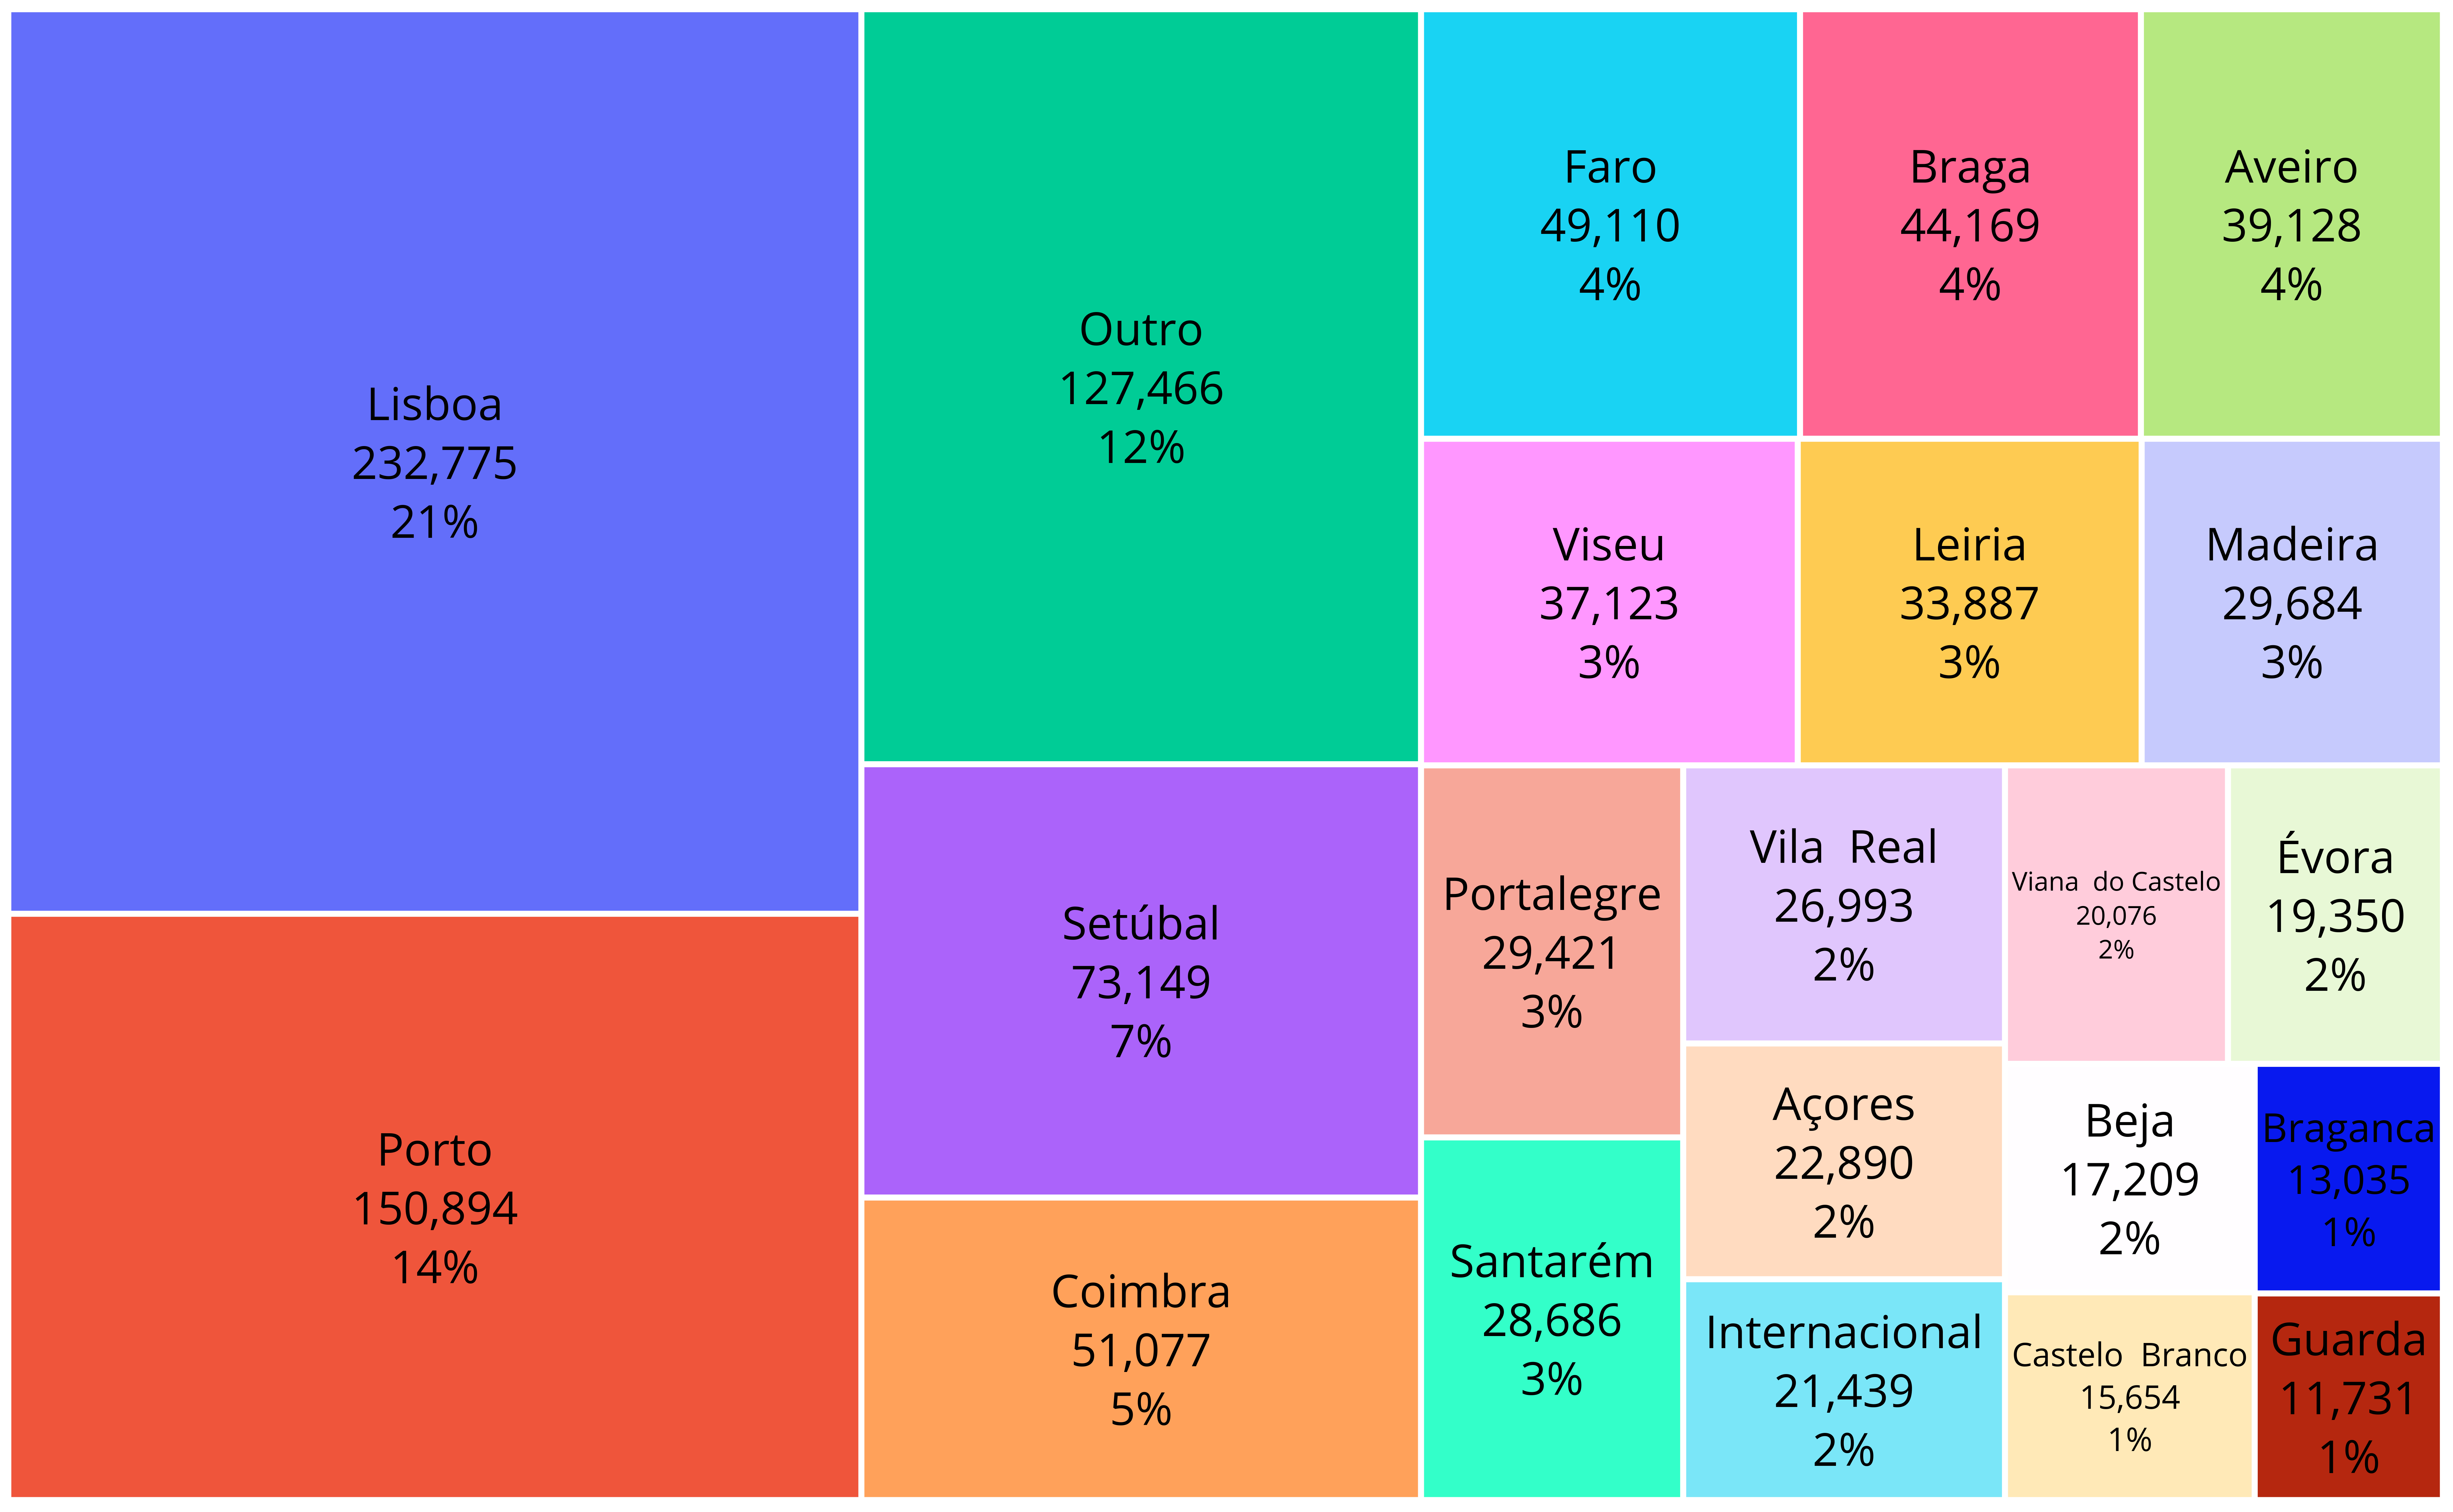
\includegraphics[width=\textwidth]{imagens/treemap_distritos.png}
	\caption{Distribuição do número de contratos públicos, por distrito, em Portugal.}
	\label{fig:distritos}
\end{figure}
\vfill 
\begin{figure}[H]
	\centering
	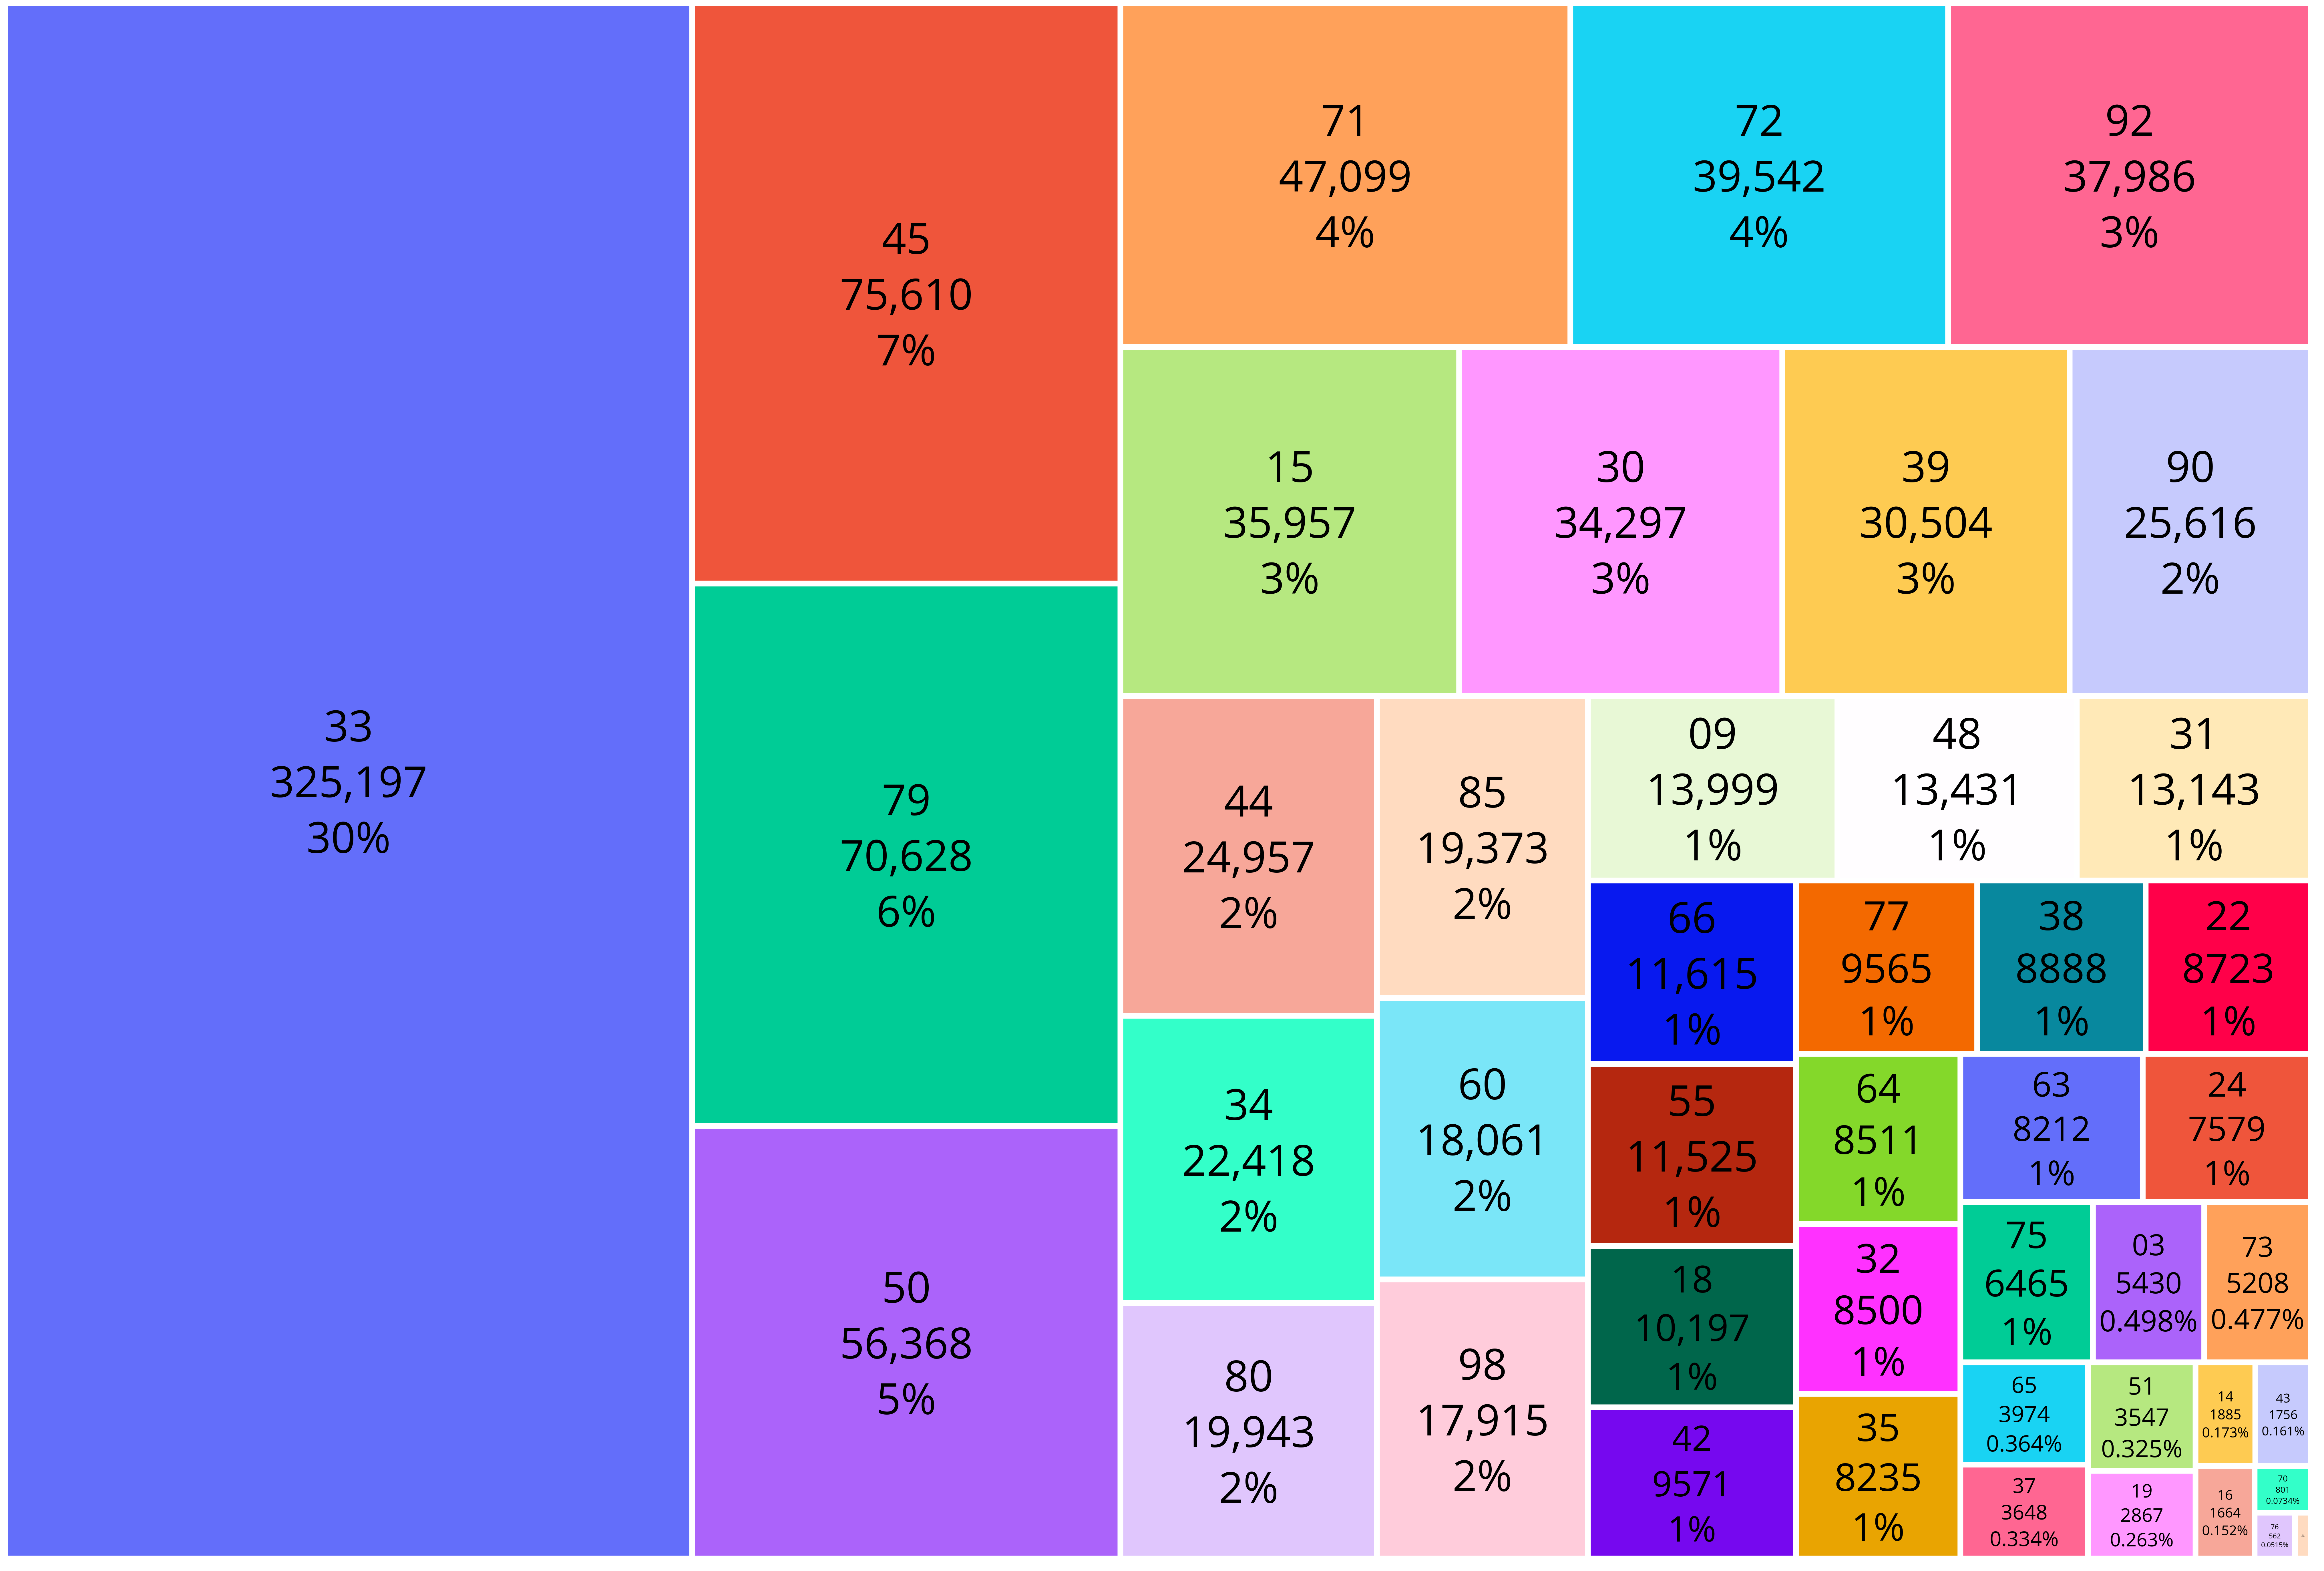
\includegraphics[width=\textwidth]{imagens/treemap_contratos.png}
	\caption{Distribuição do número de contratos públicos, por divisão do CPV.}
	\label{fig:cpvs}
\end{figure}
\vfill
\clearpage


\begin{wrapfigure}{R}{0.49\textwidth}
	\centering
	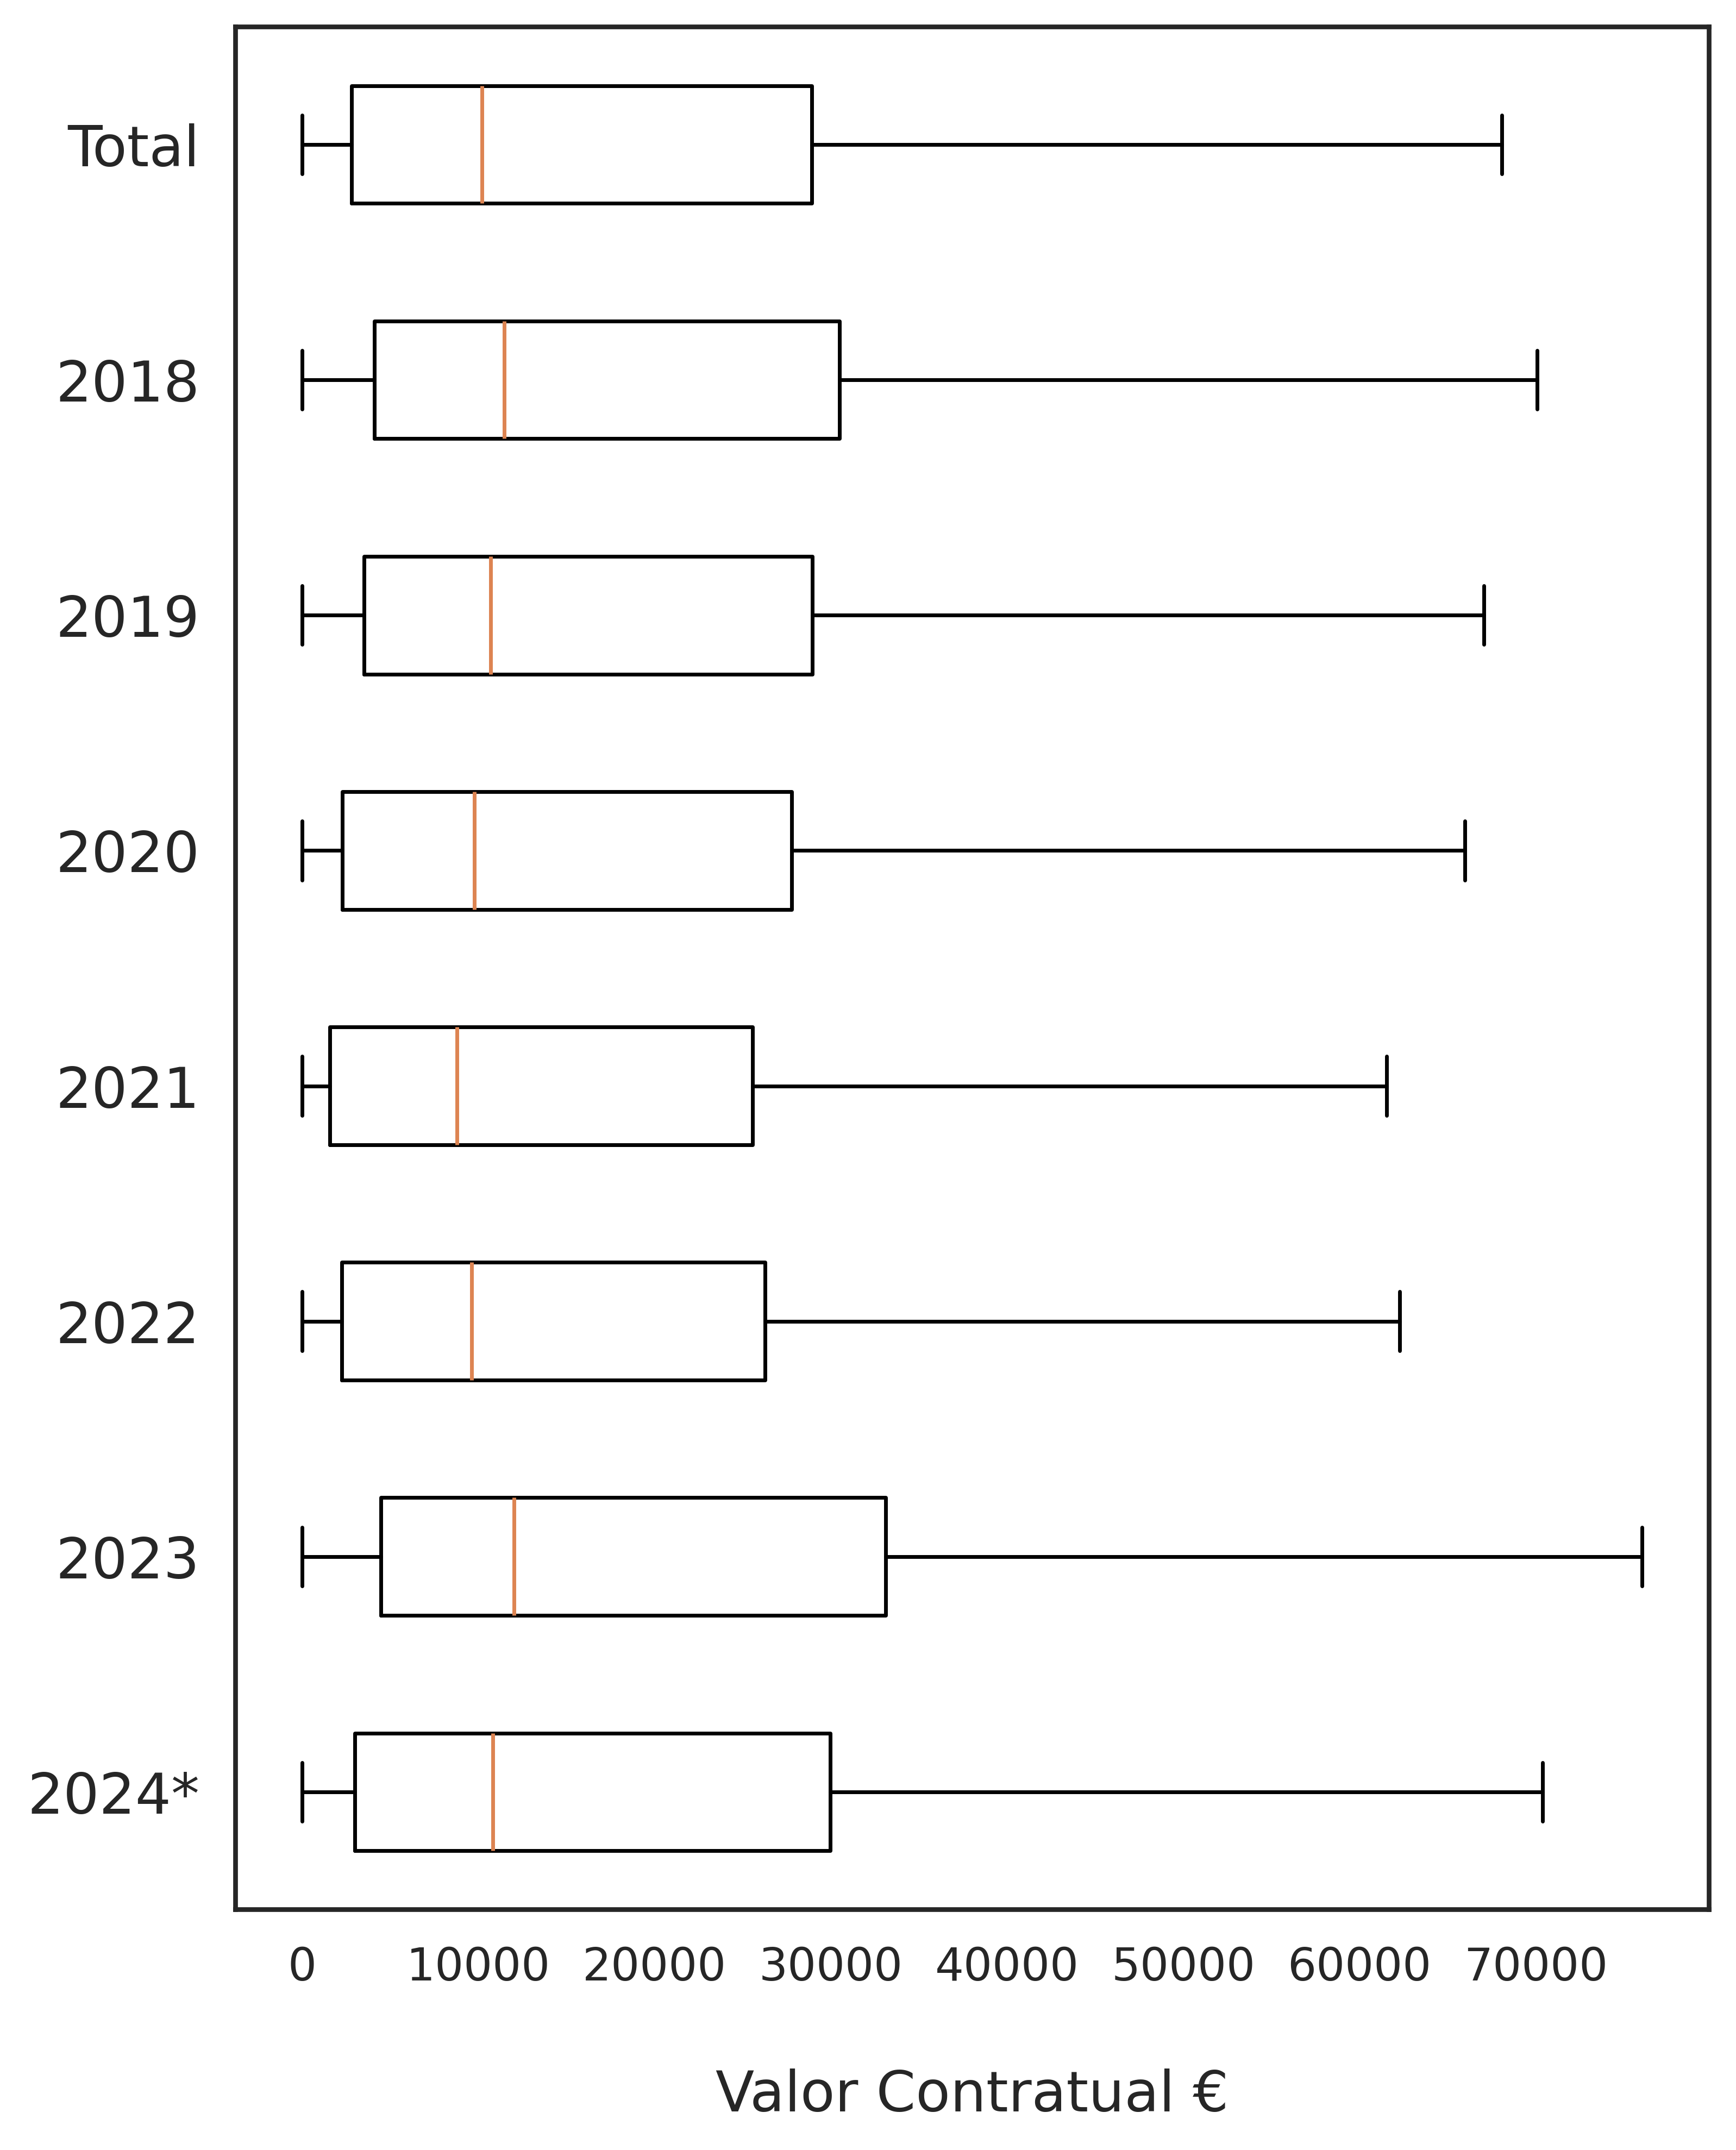
\includegraphics[width=0.49\textwidth]{imagens/precoscontr_stat.png}
	\caption{Boxplot dos preços contratuais para toda a tipologia de contratos desde 2018 até 2024}
	\label{fig:precotodos}
\end{wrapfigure}


Outra das variáveis com especial relevância e que foi considerada ao longo do projeto é o preço contratual. A Figura \ref{fig:precotodos} representa os \textit{boxplots} referentes aos preços contratuais para todos os contratos da base de dados, independentemente da tipologia de procedimento, por ano e durante o período de tempo considerado (de 2018 a 2024). É importante sublinhar que, tendo em conta que existem 2672 contratos cujo preço contratual é nulo, estes gráficos são meramente ilustrativos, correndo assim um desfasamento entre a informação apresentada e os valores reais. Pode-se observar que os valores dos 1º, 2º e 3º quartis tomam, sensivelmente, valores próximos para todos os anos. A distância interquartil é, aproximadamente, a mesma para os anos considerados e a distribuição dos valores é claramente assimétrica à direita. Porém, tendo em conta que neste cálculo são consideradas todas as tipologias de contratos e todas as divisões de CPV, esta informação não é conclusiva. Evidentemente, os valores adjudicados aos contratos referentes à construção civil (45) são mais expressivos que os referentes a serviços recreativos, culturais e desportivos (92). Por sua vez, tal como foi apresentado no capítulo anterior, existem valores contratuais máximos permitidos mediante a tipologia de contrato. Desta forma, é natural que exista um elevado número de \textit{outliers}, não representados na Figura \ref{fig:precotodos}. \\
Ao longo deste estágio foram apenas consideradas duas tipologias de contratos: Ajustes Diretos em Regime Geral e Concursos Públicos. Assim, é oportuno incluir alguma descrição estatística destes dois casos. Foram construídos  \textit{boxplots} como representações gráficas relativas ao número de contratos e respetivo preço contratual total, por ano. Os resultados encontram-se nas Figuras \ref{fig:precocps}, \ref{fig:precocps1} e \ref{fig:precocps2}, para concursos públicos e nas Figuras \ref{fig:precoad}, \ref{fig:precoad1} e \ref{fig:precoad2}, para ajustes diretos em regime geral. 

Deste modo, possível observar que os valores contratuais dos concursos públicos, tal como observado na Figura \ref{fig:precocps}, são substancialmente superiores aos dos ajustes diretos, tal como ilustrado na Figura \ref{fig:precoad}. Apesar do número de contratos celebrados por ano para concursos públicos, tal como indicado na Figura \ref{fig:precocps1}, ser sempre inferior ao de ajustes diretos - Figura \ref{fig:precoad1} -, o valor adjudicado, por ano, foi sempre superior ao dos ajustes diretos. Deste modo, pode concluir-se que os valores contratuais de concursos públicos tem, necessariamente, de ser superiores. Em ambos os casos, as distribuições dos valores contratuais são assimétricas. 

No caso dos concursos públicos, 23\% dos contratos celebrados referem-se à aquisição de equipamento médico e 17\% a obras de contrução civil (ver Figura \ref{fig:cpcpv}), sendo que cerca de 25\% são celebrados no distrito de Lisboa, 10\% no Porto e 11\% em distritos indeterminados (ver Figura \ref{fig:cploc}). Relativamente a ajustes diretos, existe uma predominância de contratos referentes à aquisição de equipamento médico, totalizando 28\% dos contratos celebrados (ver Figura \ref{fig:adcpv}), com maior destaque para os distritos de Lisboa, com 23\% e Porto, com 17\%  (ver Figura \ref{fig:adloc}).

\vfill

\begin{figure}[H]
	\centering
	\begin{minipage}{0.31\linewidth}
		%\centering  % redundant
		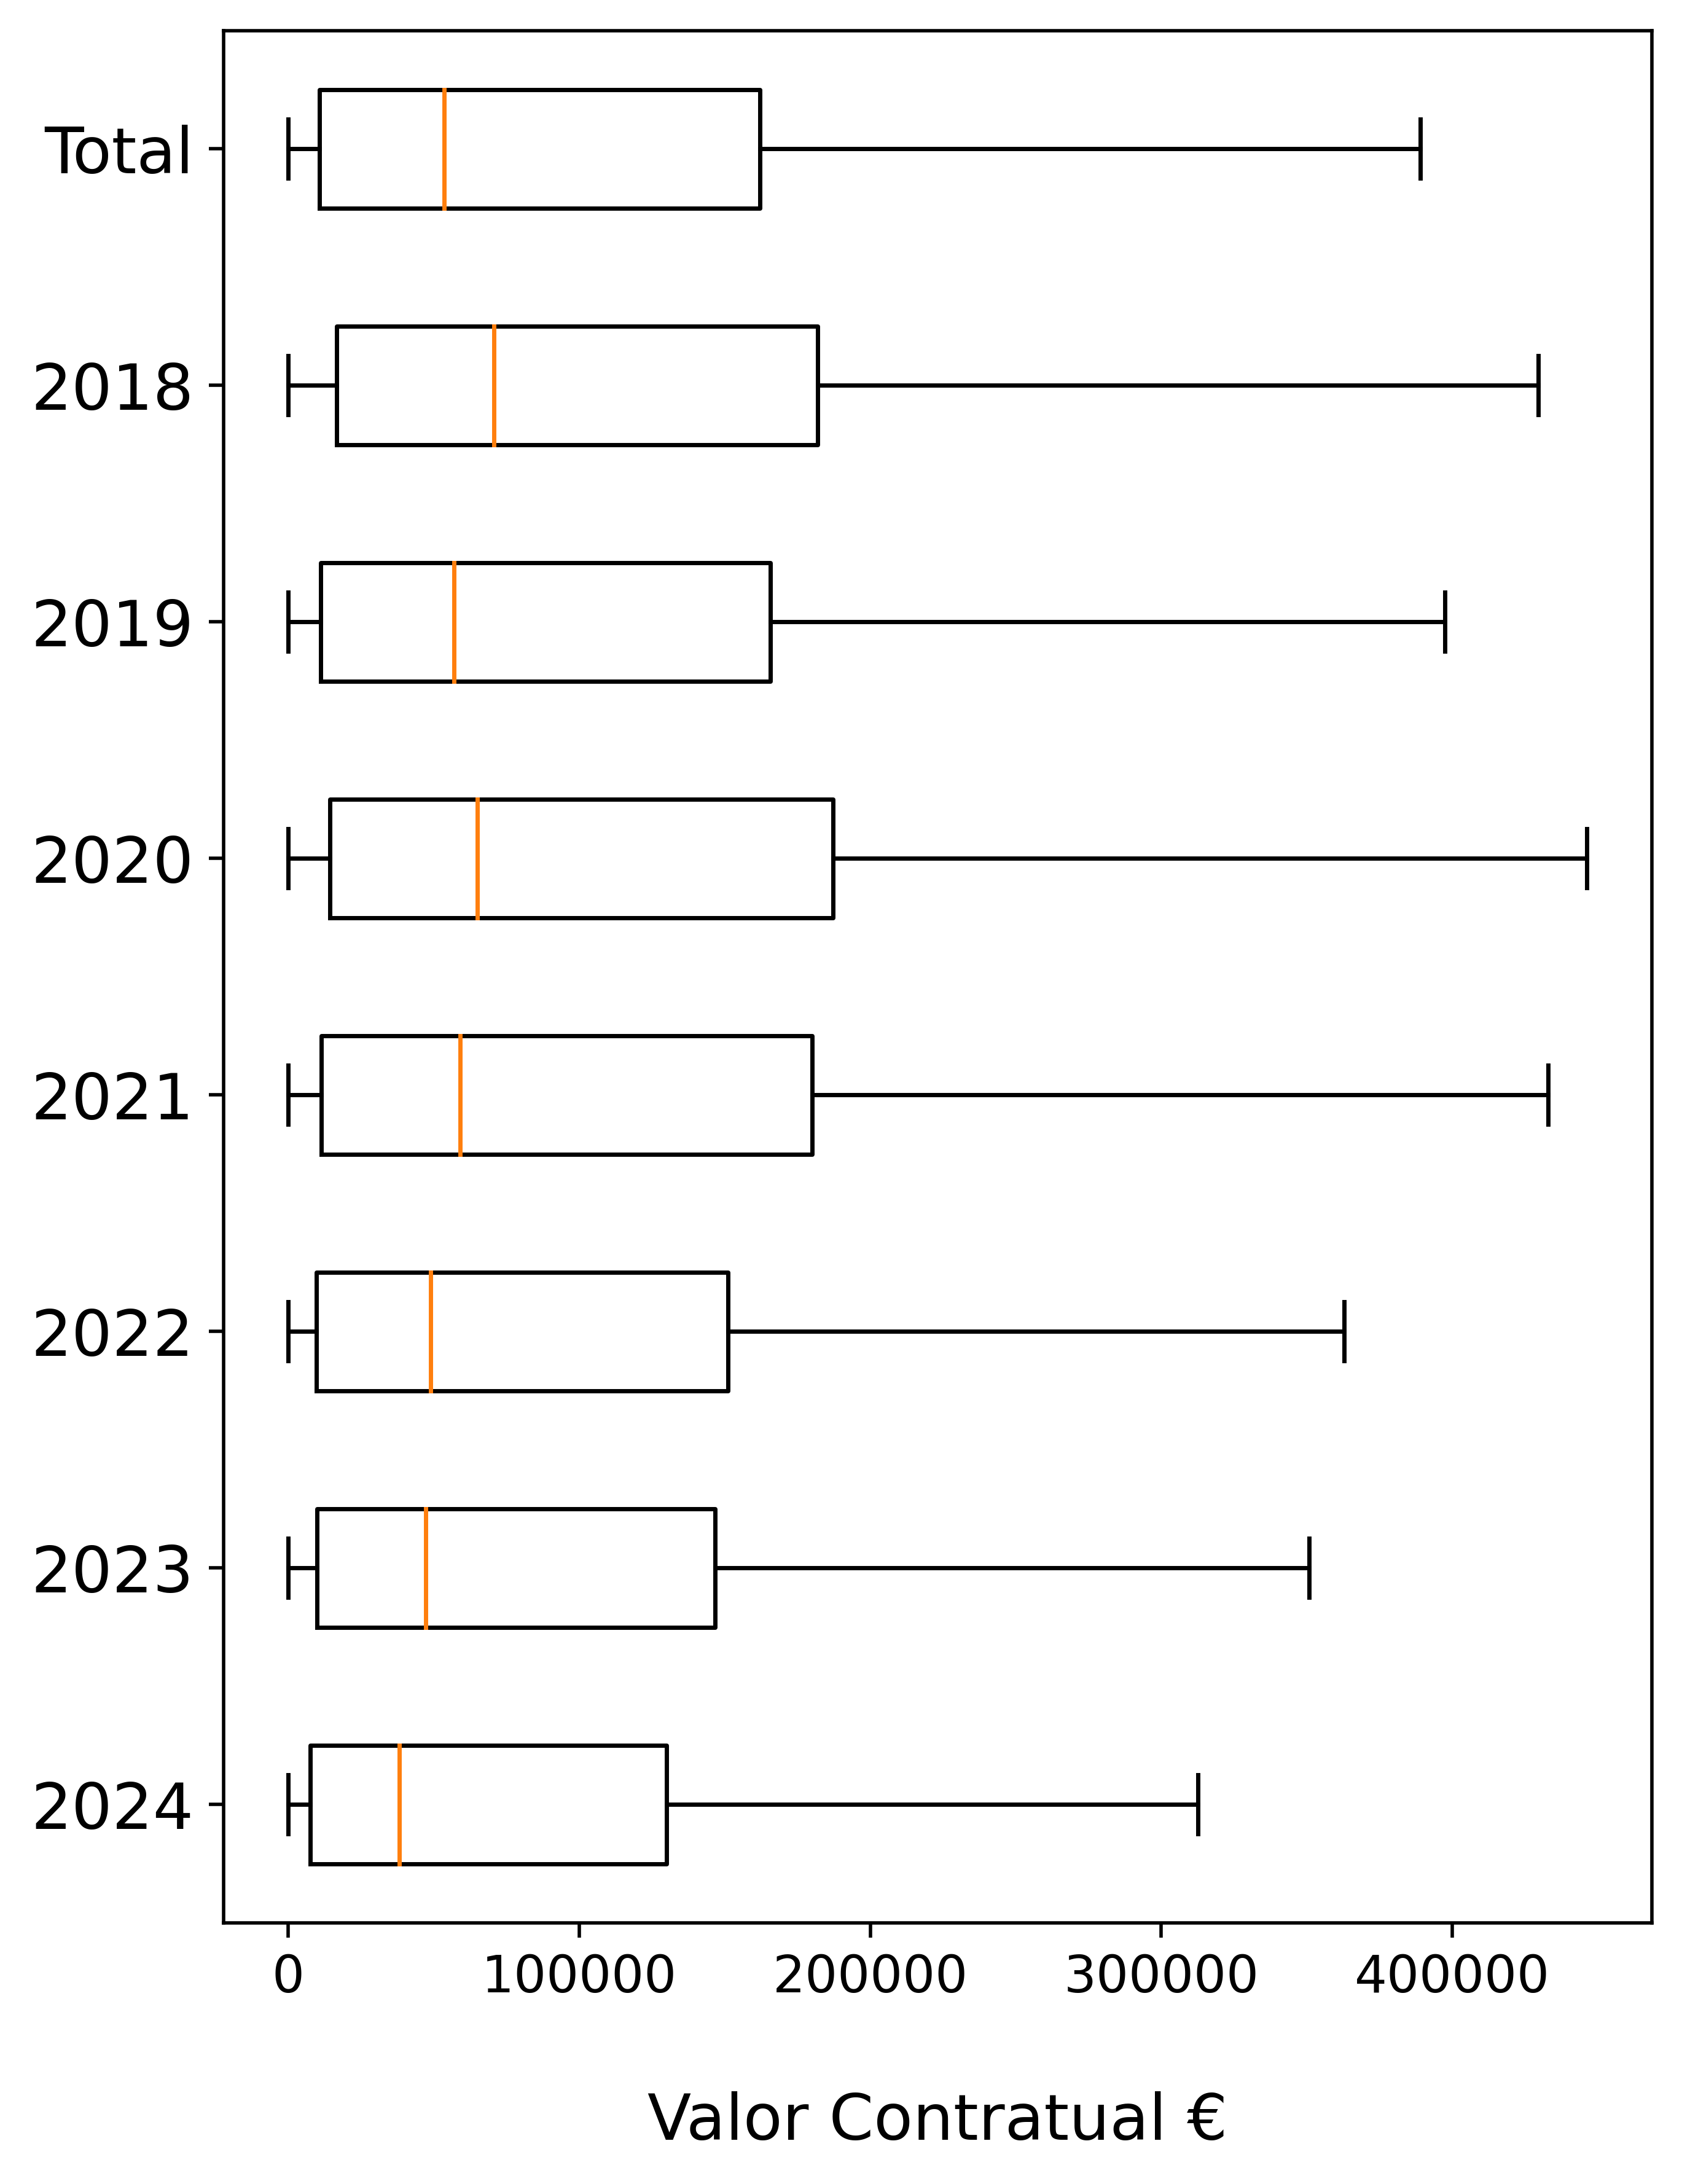
\includegraphics[width=\textwidth]{imagens/concpub_stat.png}
		\caption{Boxplot dos preços contratuais para concursos públicos entre 2018 até 2024.}
		\label{fig:precocps}
	\end{minipage}
	\hfill
	\begin{minipage}{.31\linewidth}
		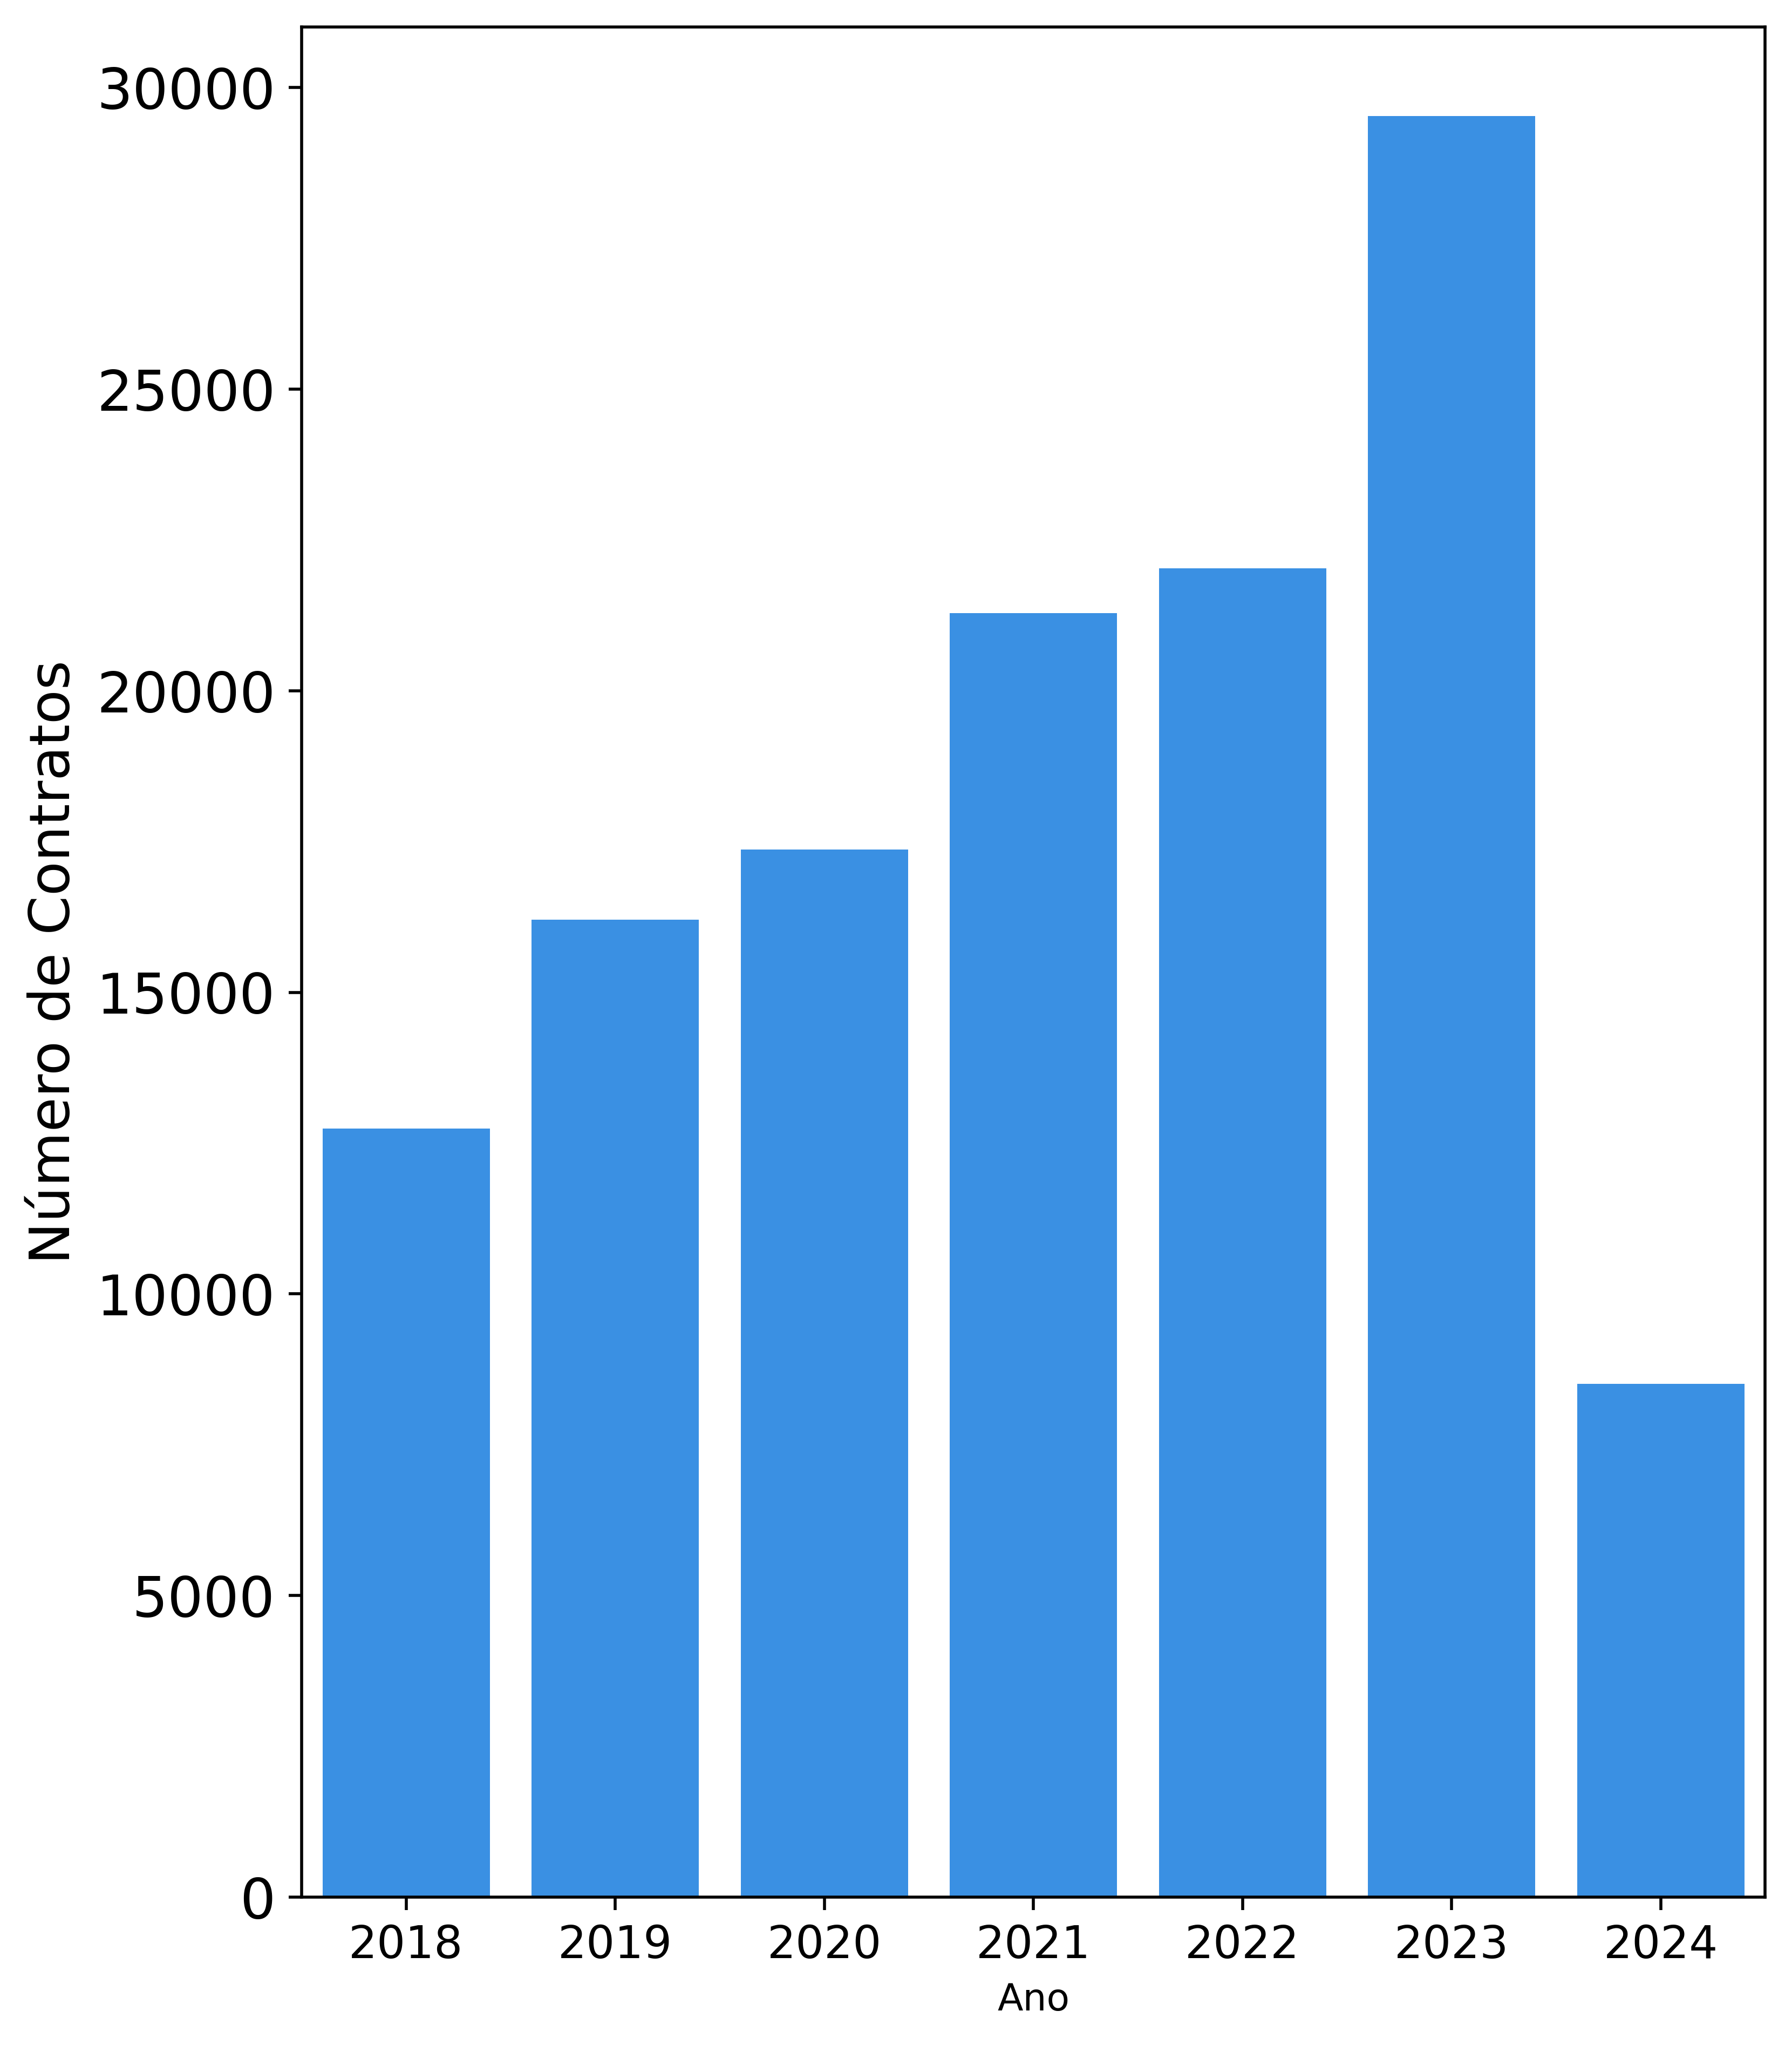
\includegraphics[width=\linewidth]{imagens/cpub_nrcontr.png}
		\caption{Número de concursos públicos celebrados, entre 2018 e 2024.}
		\label{fig:precocps1}
	\end{minipage}
	\hfill
	\begin{minipage}{.31\linewidth}
		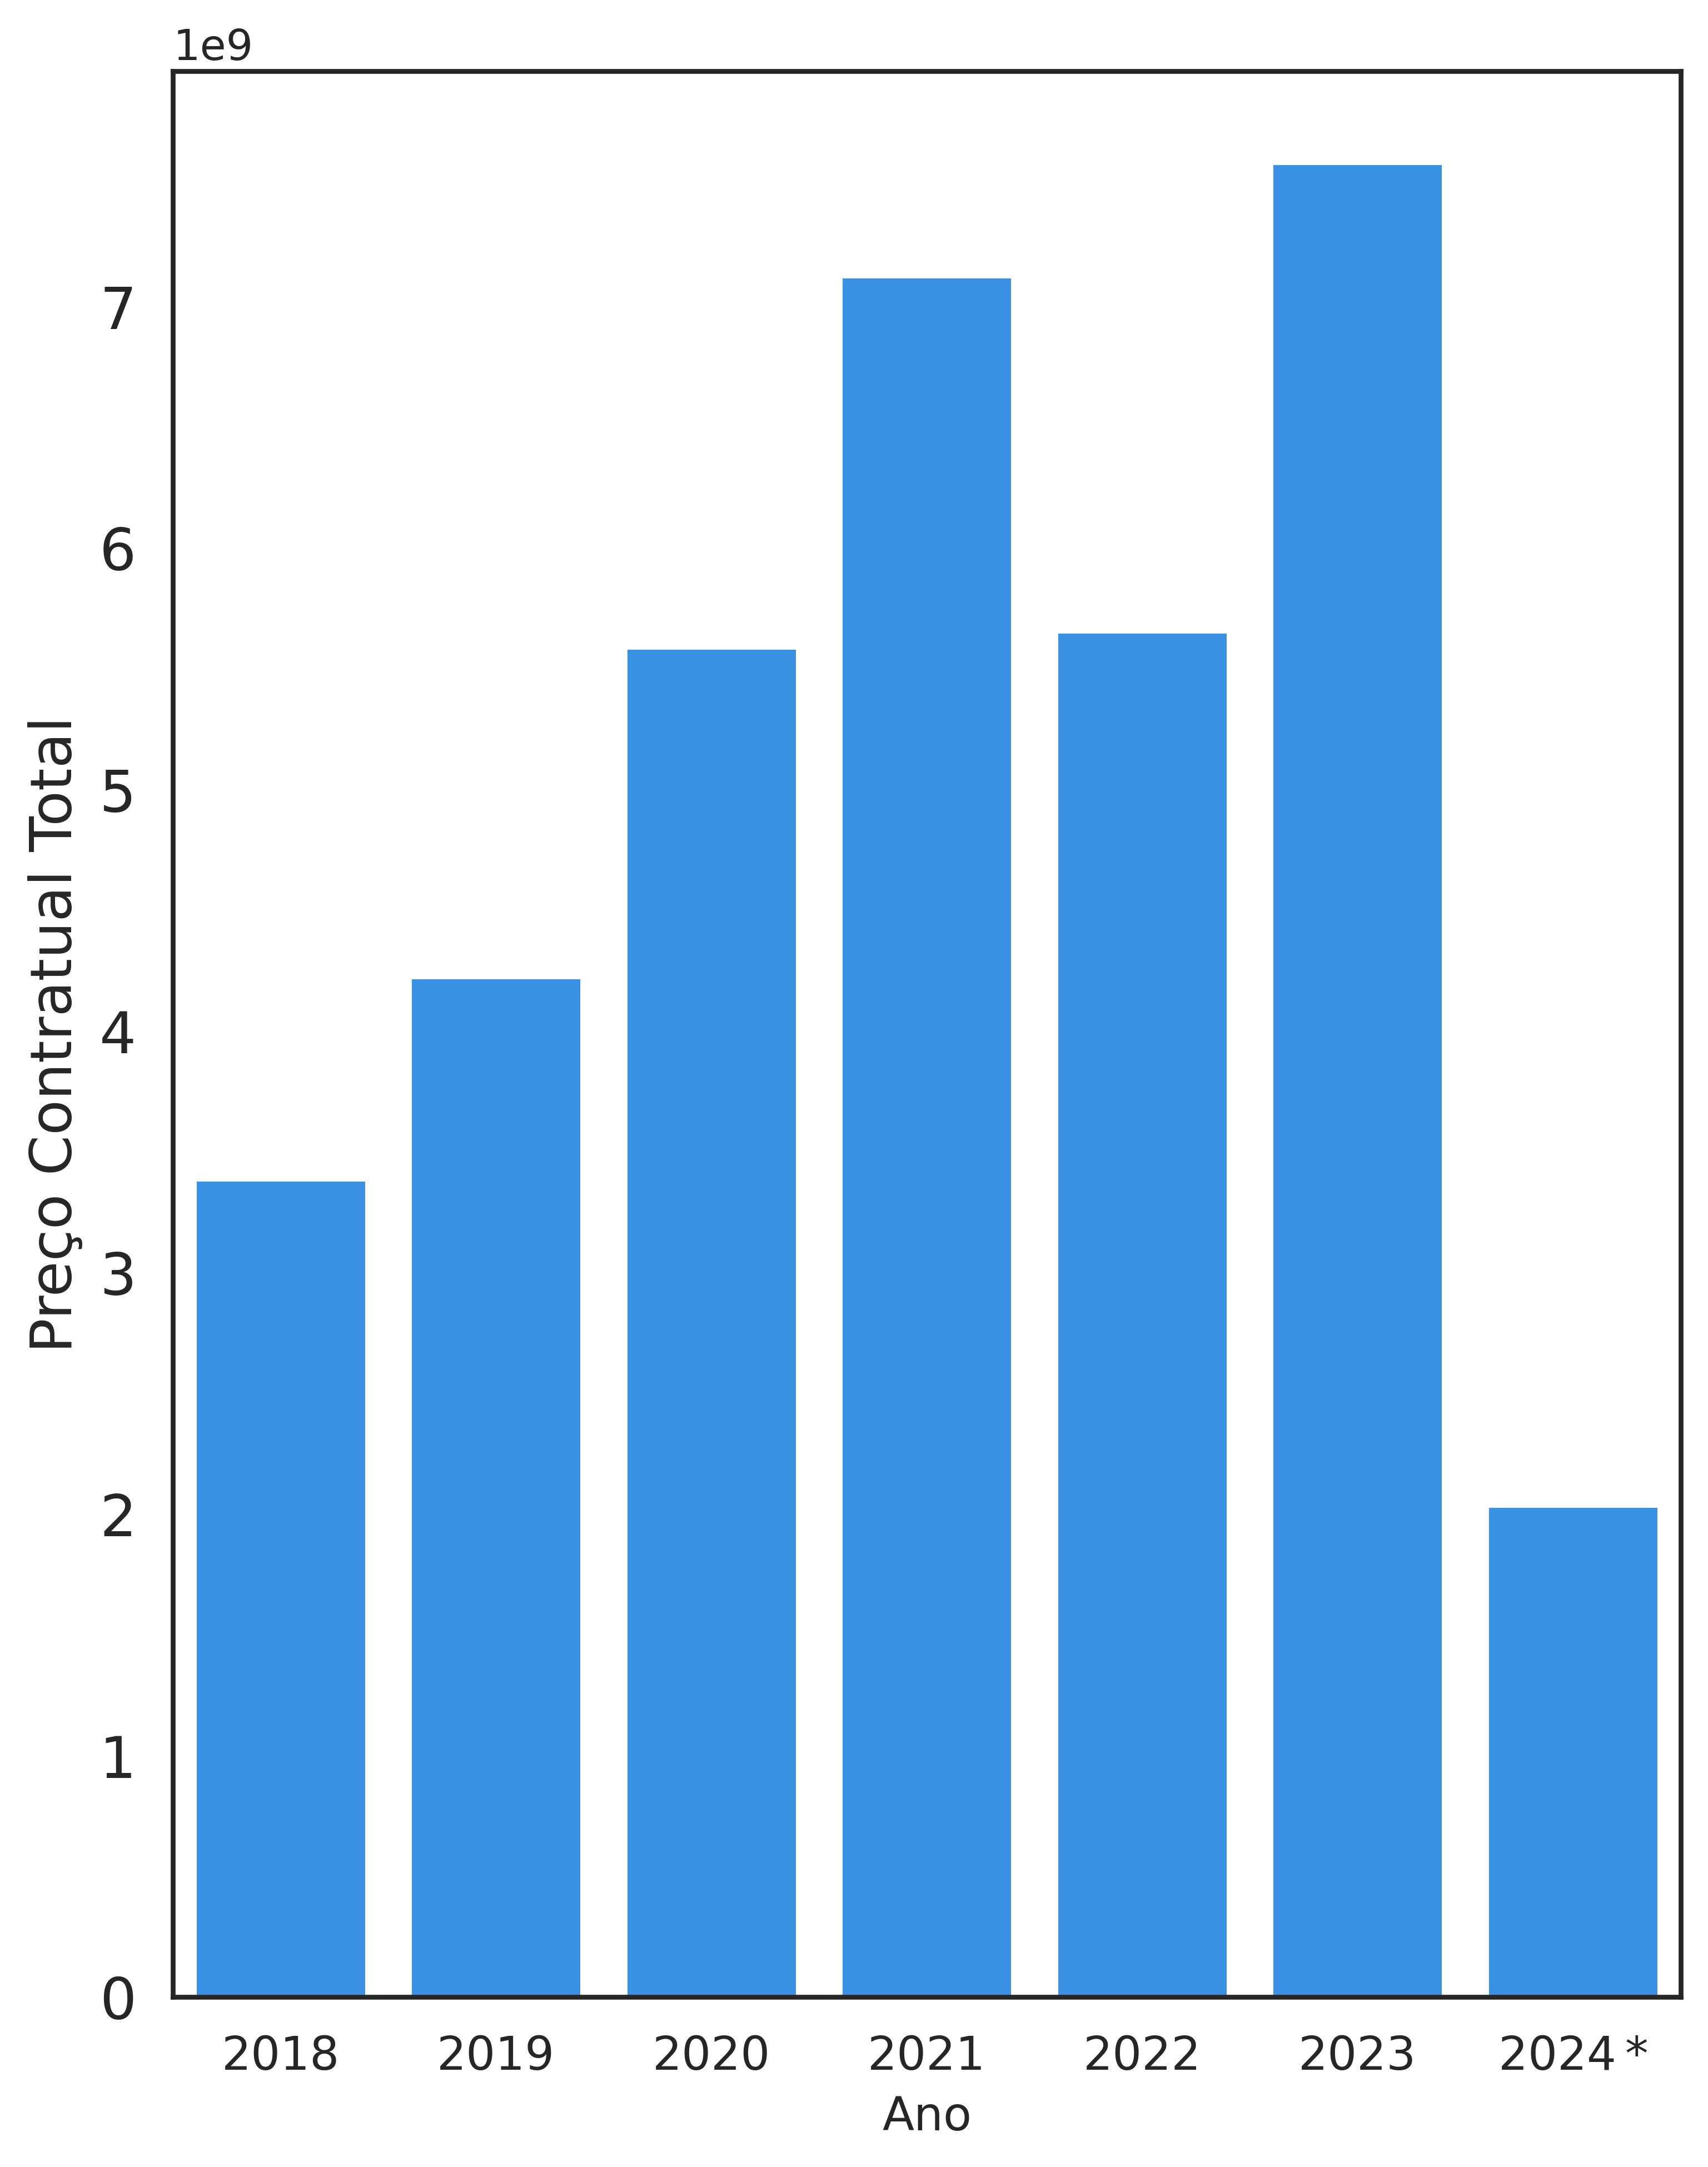
\includegraphics[width=\linewidth]{imagens/cpub_price.png}
		\caption{Preço contratual total, entre 2018 e 2024, para concursos públicos.}
		\label{fig:precocps2}
	\end{minipage}
\end{figure}

\vfill

\begin{figure}[H]
	\centering
	\begin{minipage}{.31\linewidth}
		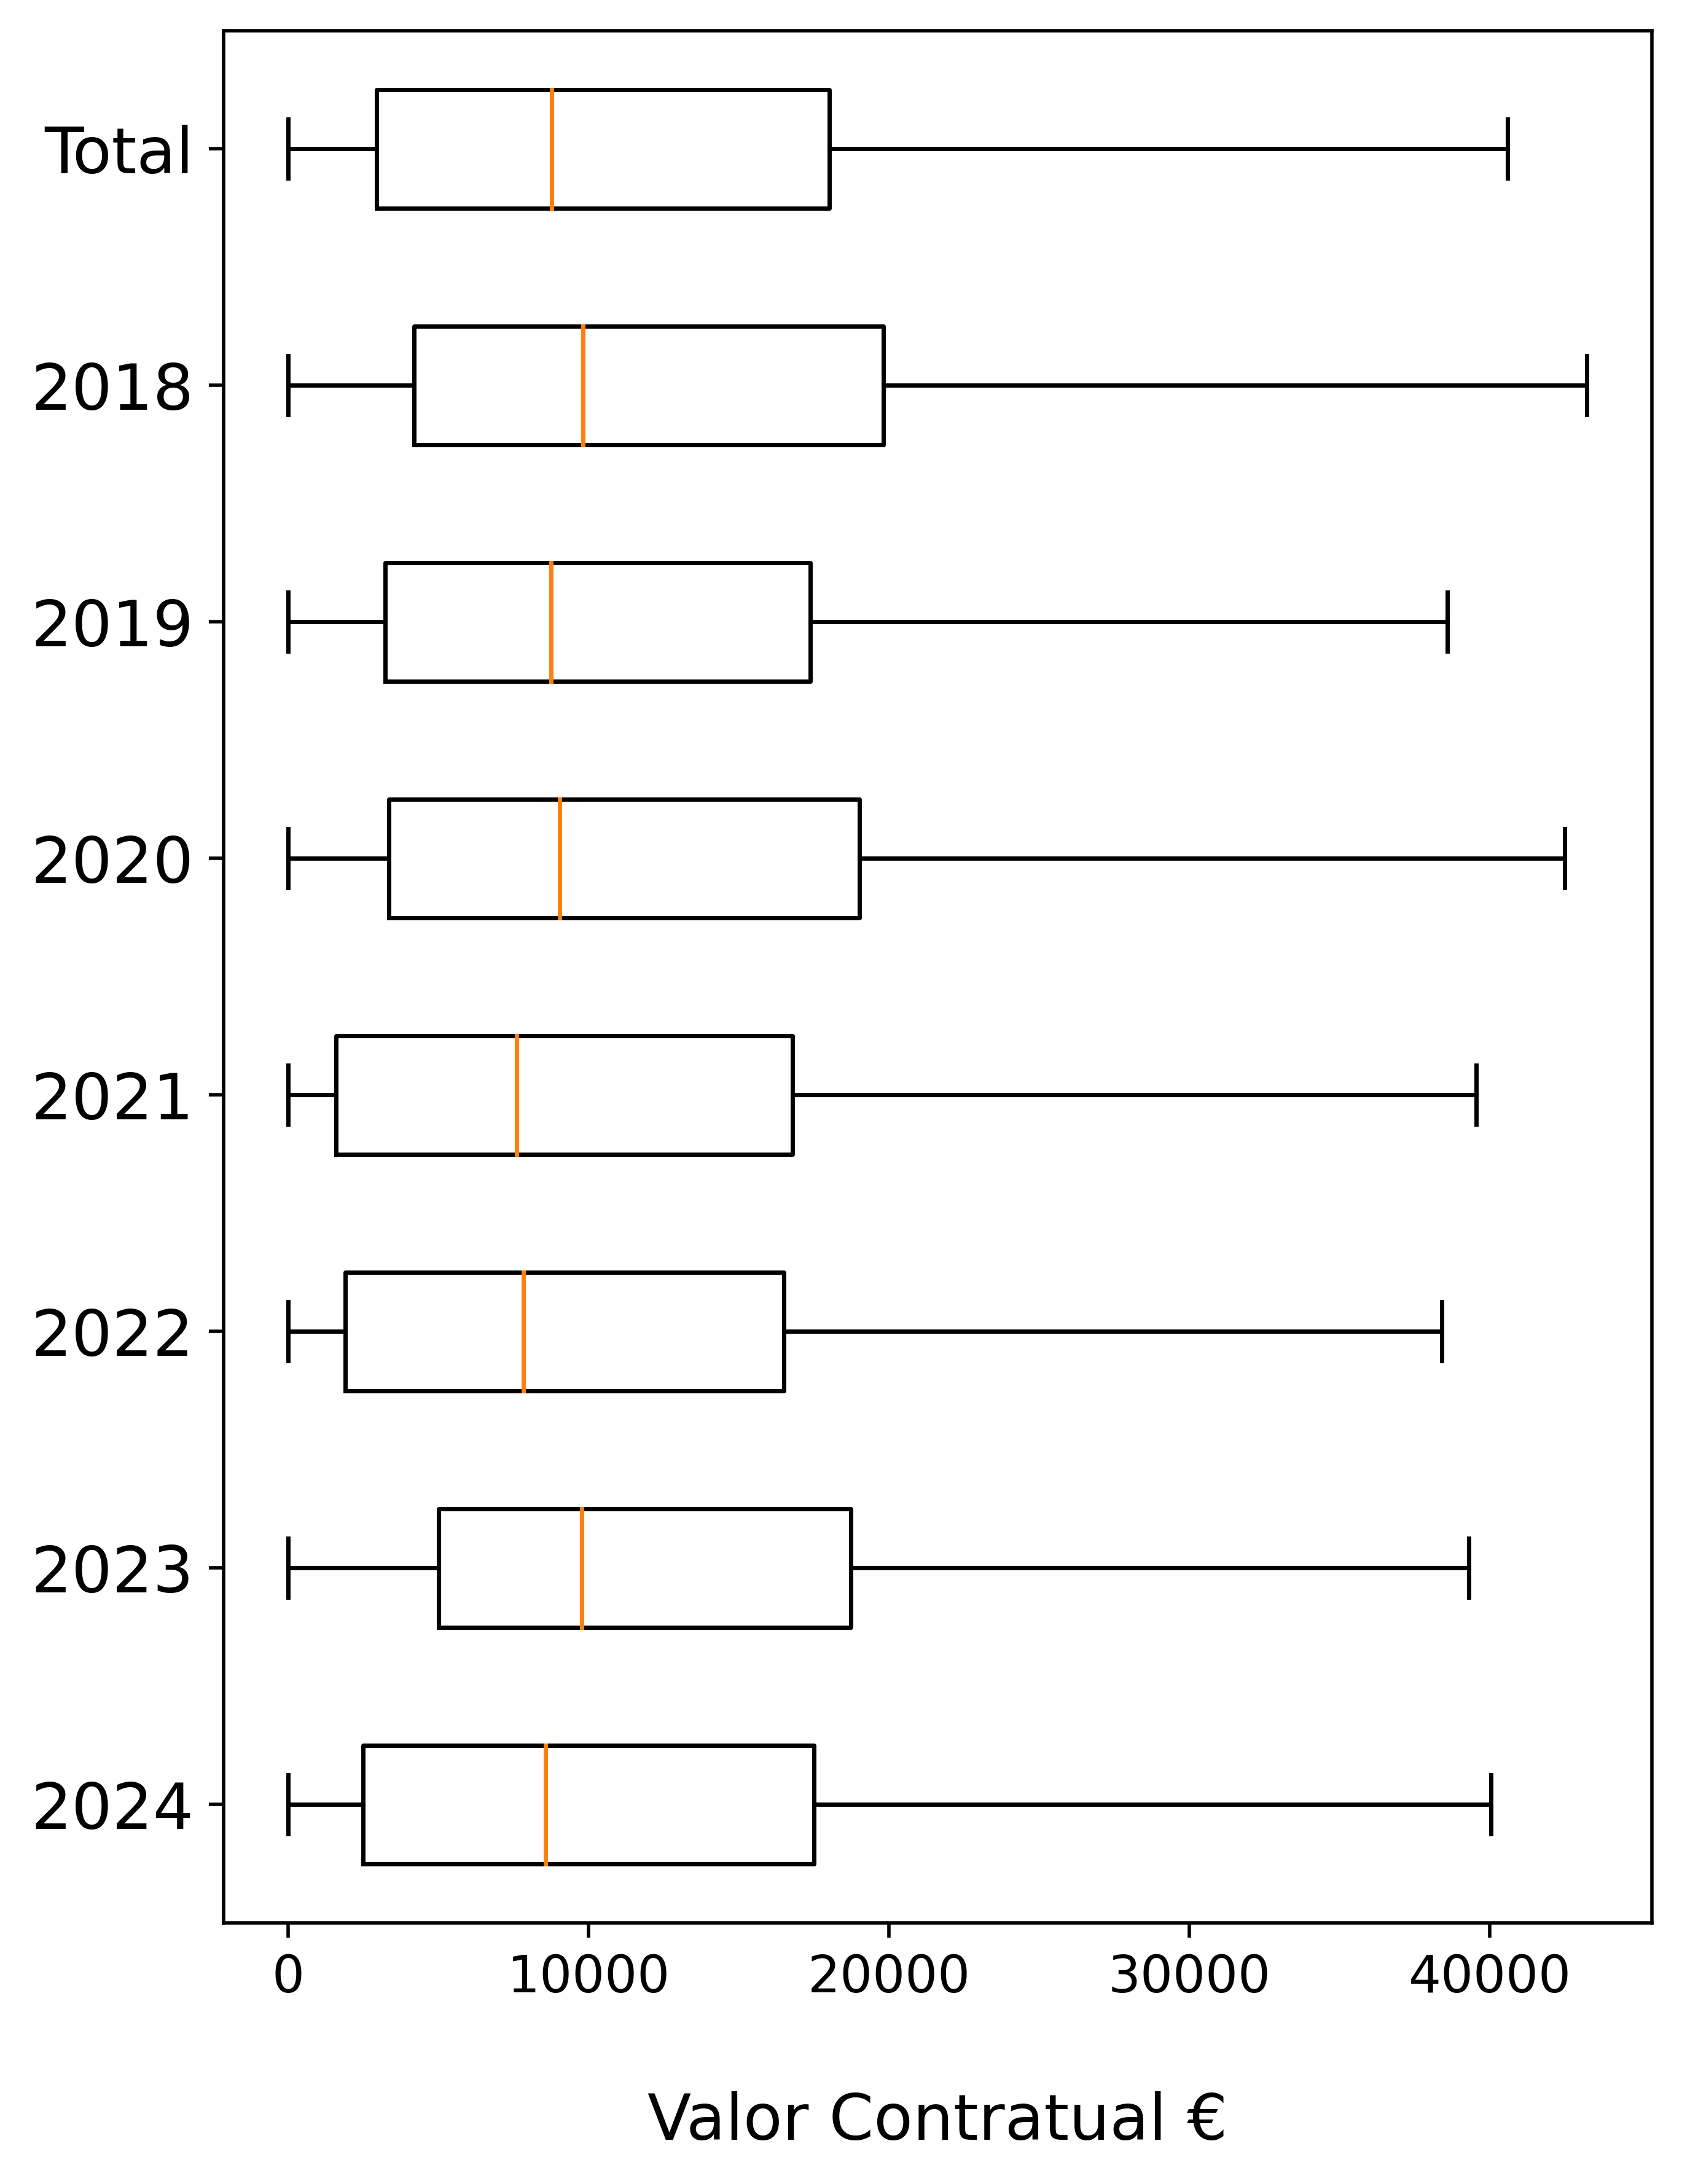
\includegraphics[width=\linewidth]{imagens/adir_stat.png}
		\caption{Boxplot dos preços contratuais de ajustes diretos celebrados, entre 2018 e 2024.}
		\label{fig:precoad}
	\end{minipage}
	\hfill
	\begin{minipage}{0.31\linewidth}
		%\centering  % redundant
		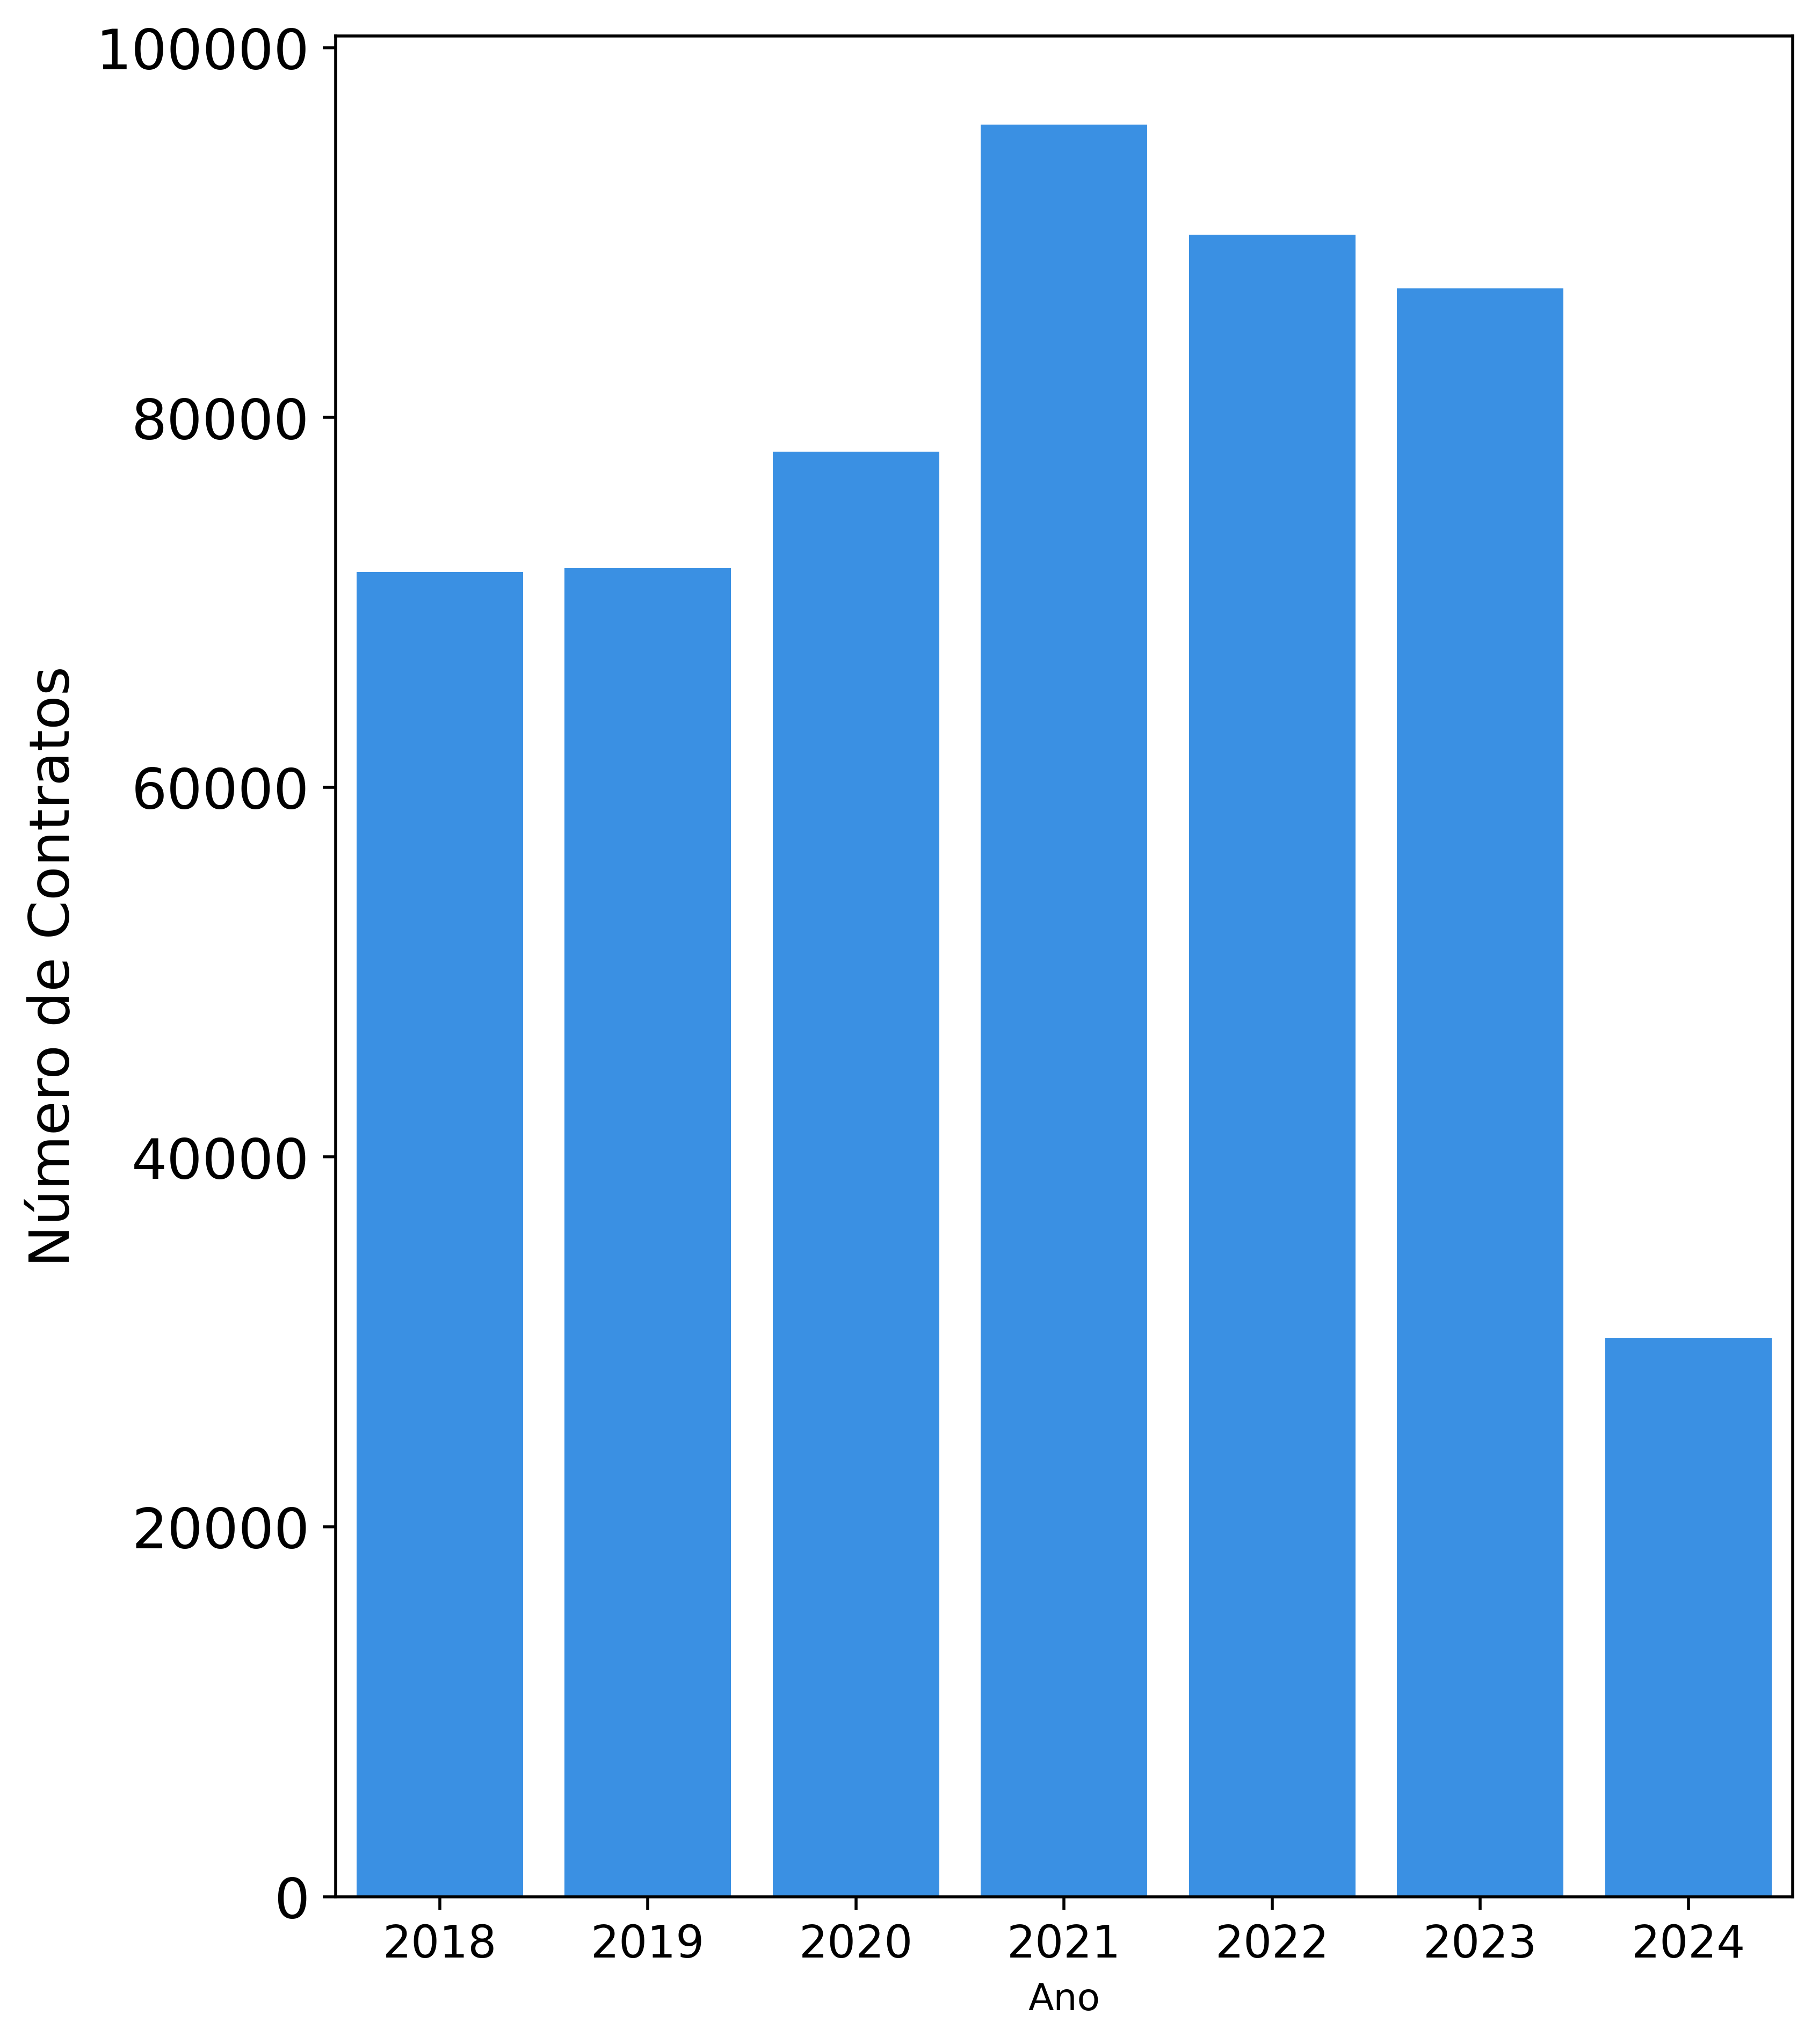
\includegraphics[width=\linewidth]{imagens/adir_nrcontr.png}
		\caption{Número de ajustes diretos celebrados, entre 2018 e 2024.}
		\label{fig:precoad1}
	\end{minipage}
	\hfill
	\begin{minipage}{.31\linewidth}
		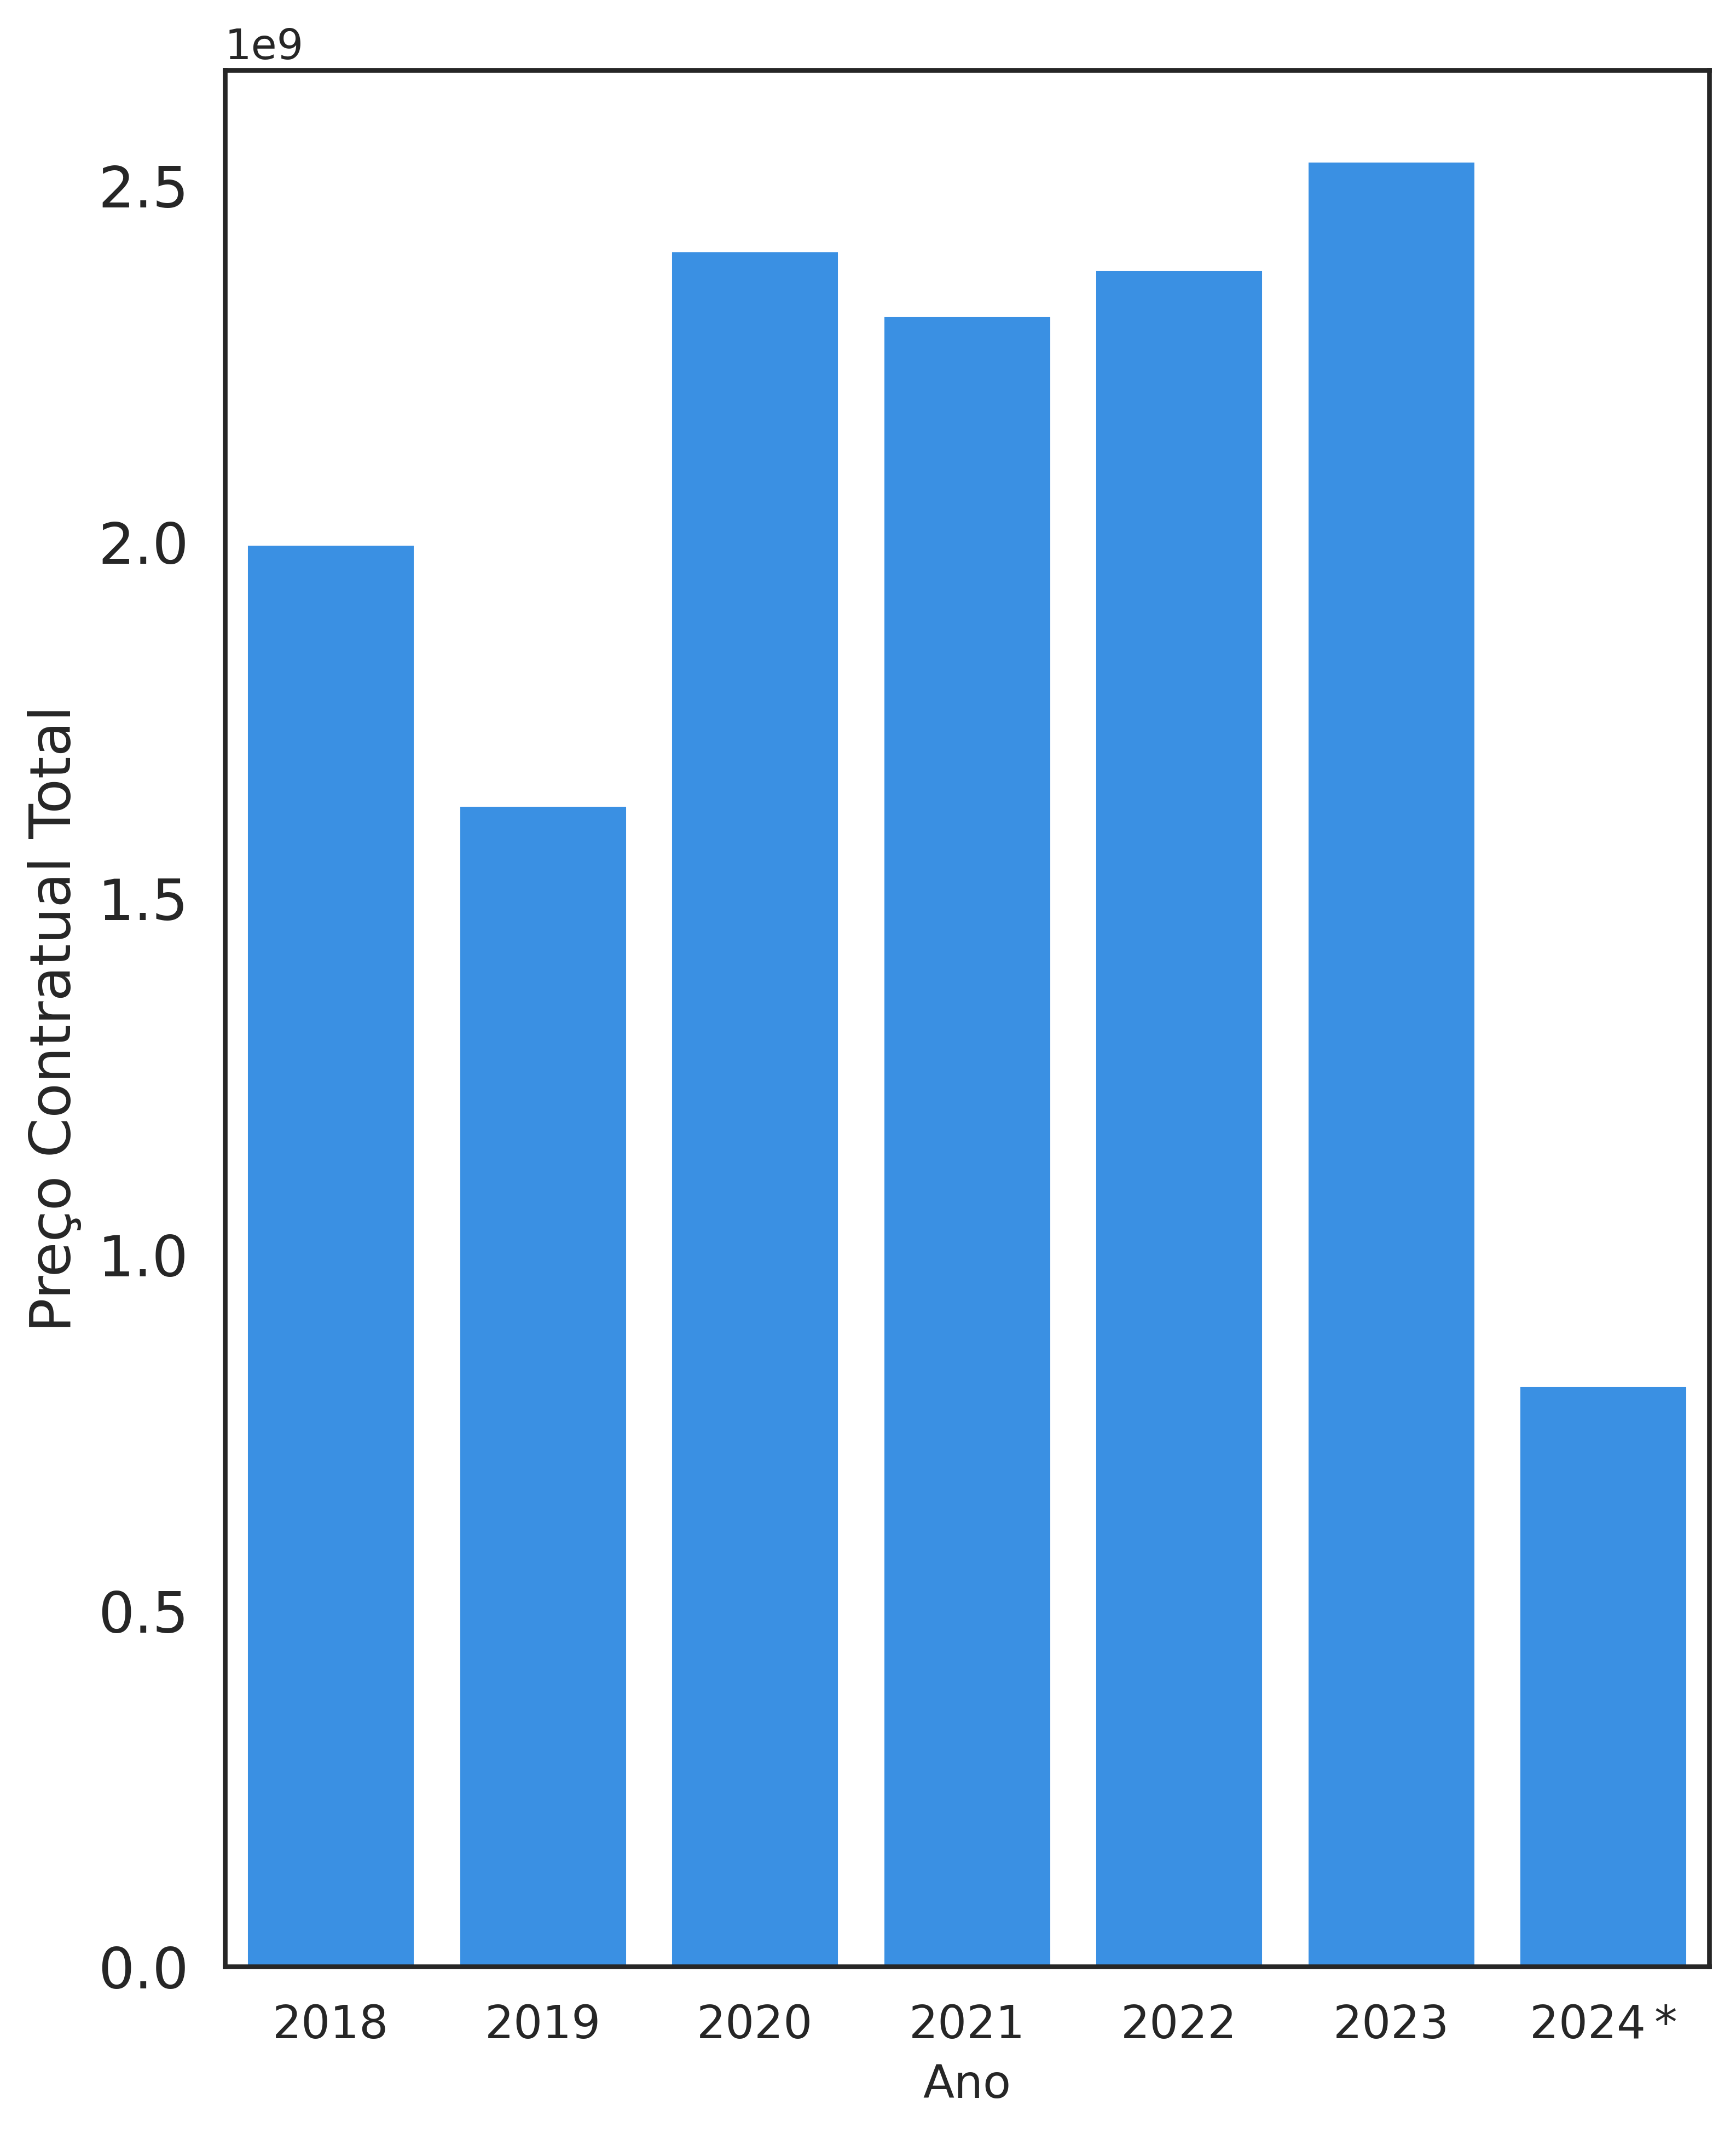
\includegraphics[width=\linewidth]{imagens/adir_price.png}
		\caption{Preço contratual total, entre 2018 e 2024, para ajustes diretos.}
		\label{fig:precoad2}
	\end{minipage}
\end{figure}


\clearpage
\begin{figure}[H]
	\centering
	
	\begin{minipage}[t]{0.49\textwidth}
		\centering
		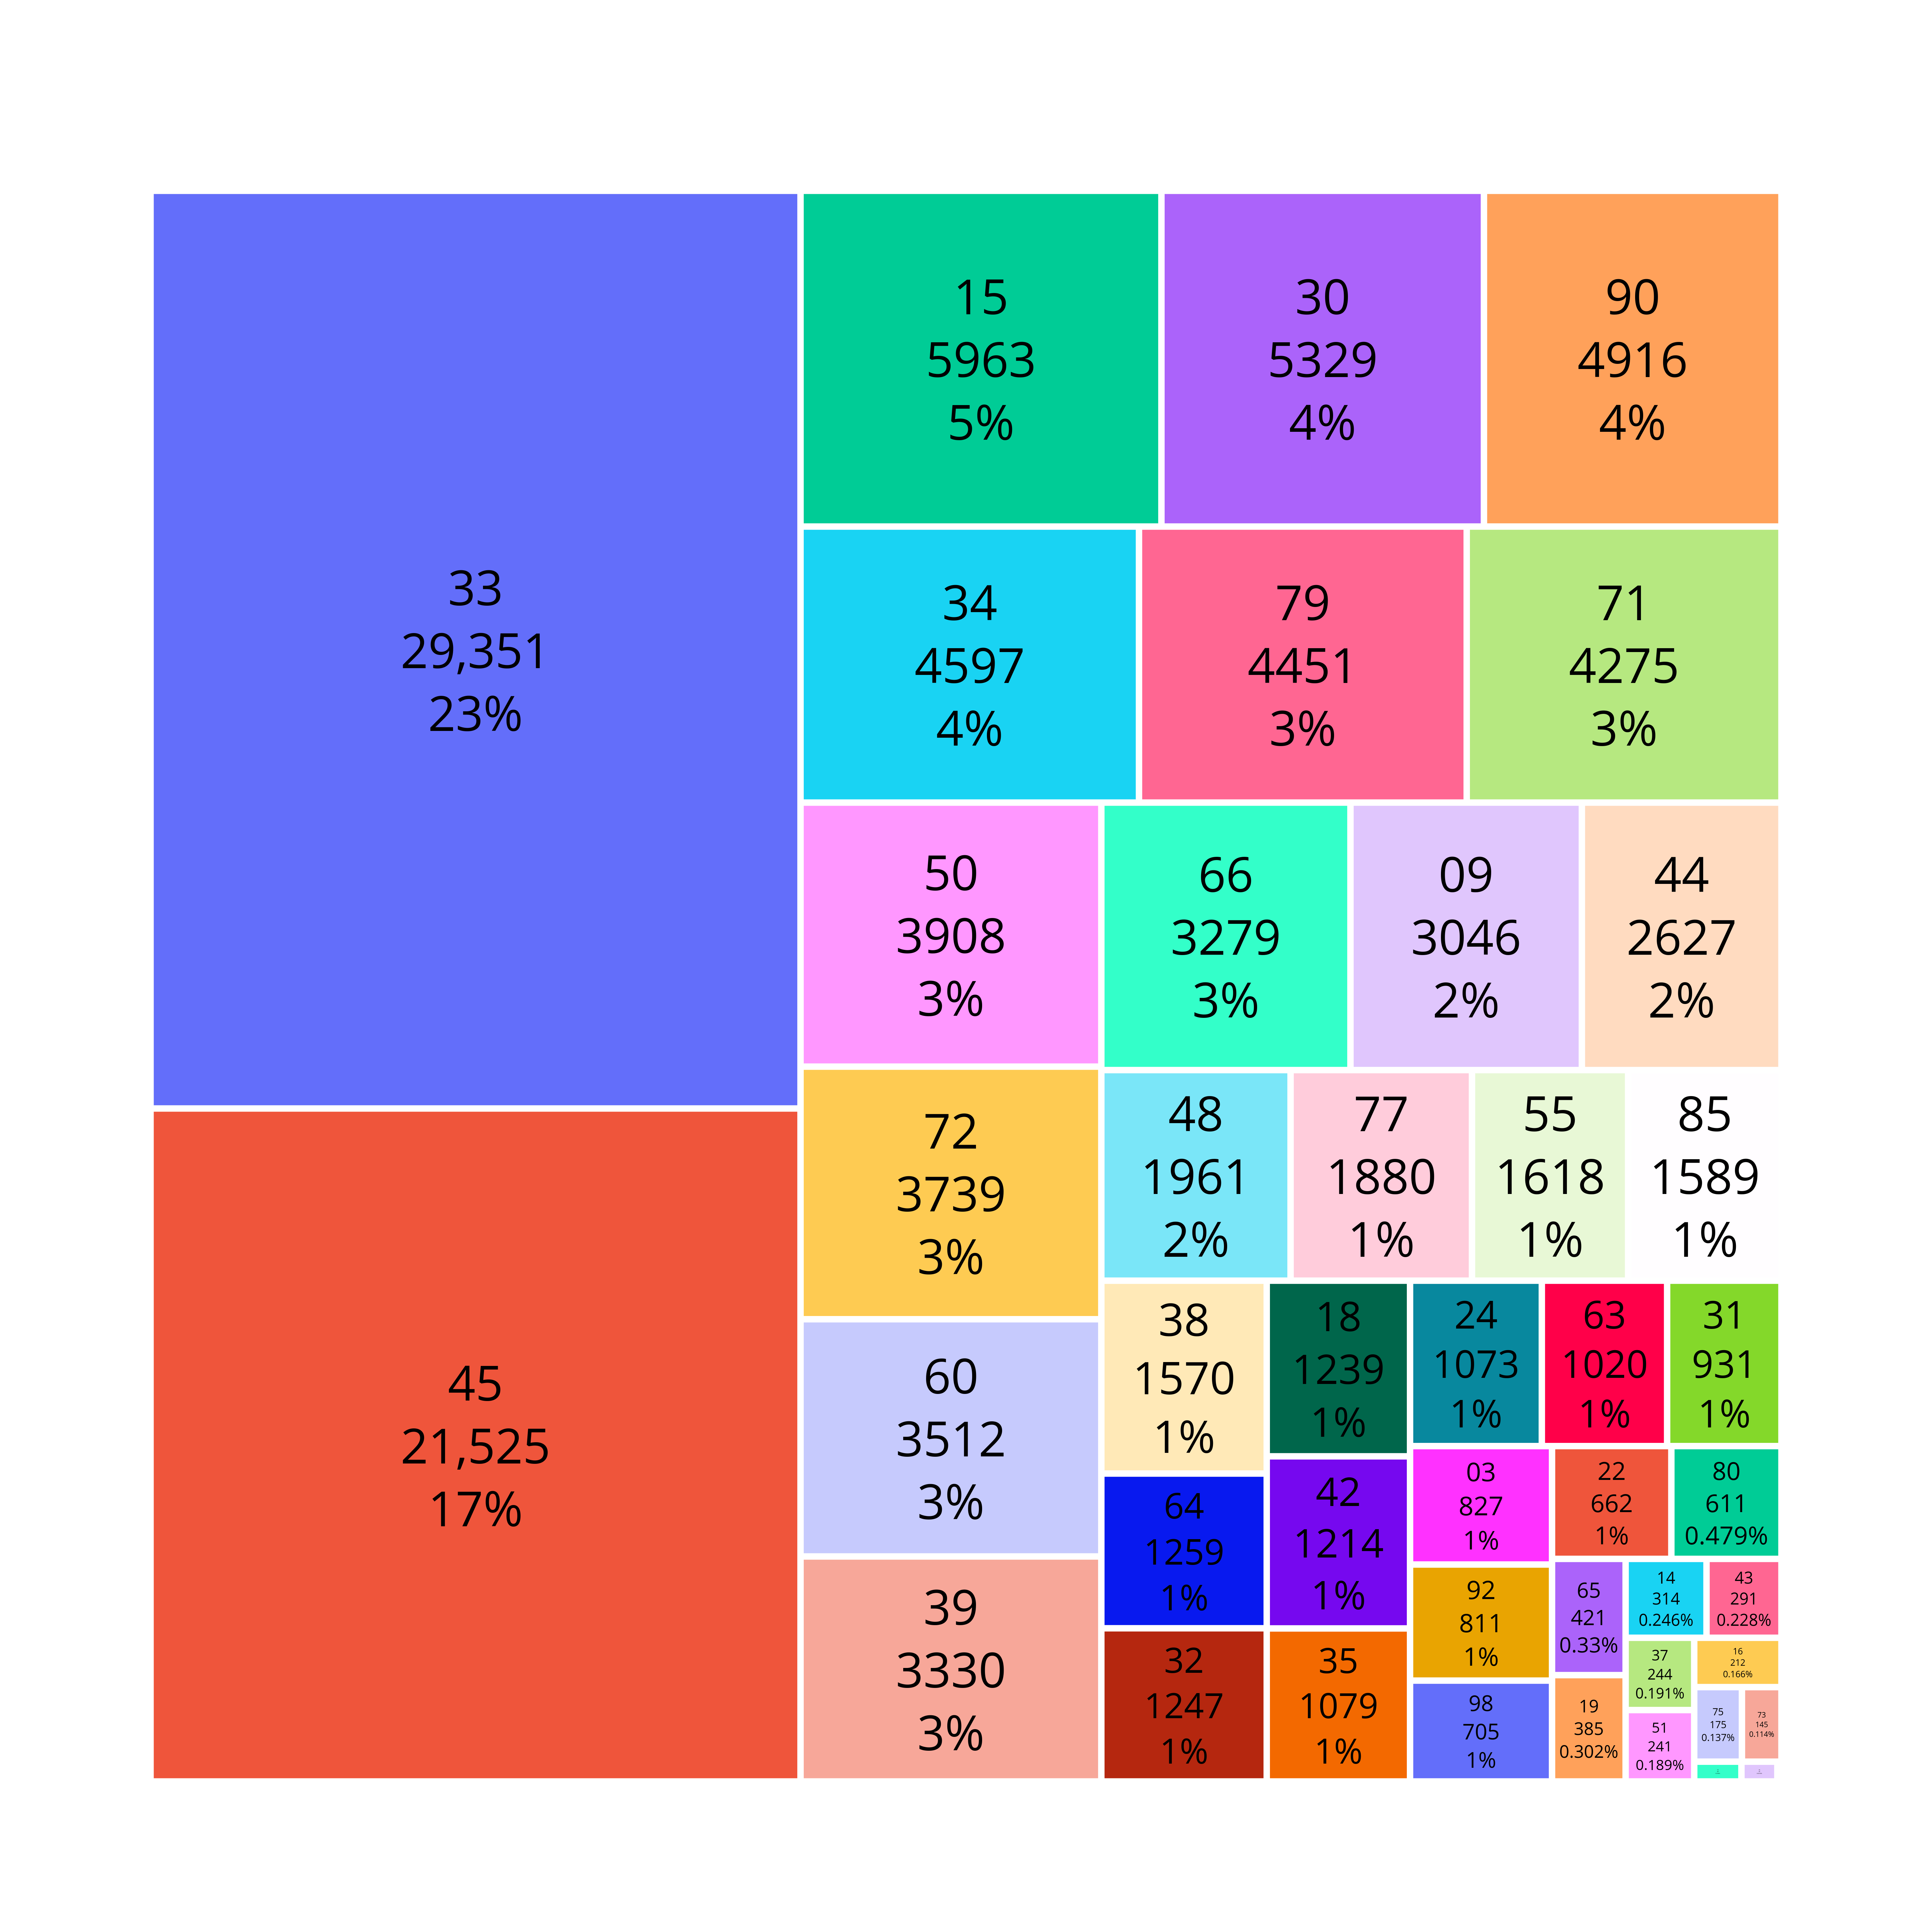
\includegraphics[width=\textwidth]{imagens/treemap_cpub.png}
		\caption{Distribuição do número de concursos públicos, por divisão de CPV.}
		\label{fig:cpcpv}
	\end{minipage}
	\hfill
	\begin{minipage}[t]{0.49\textwidth}
		\centering
		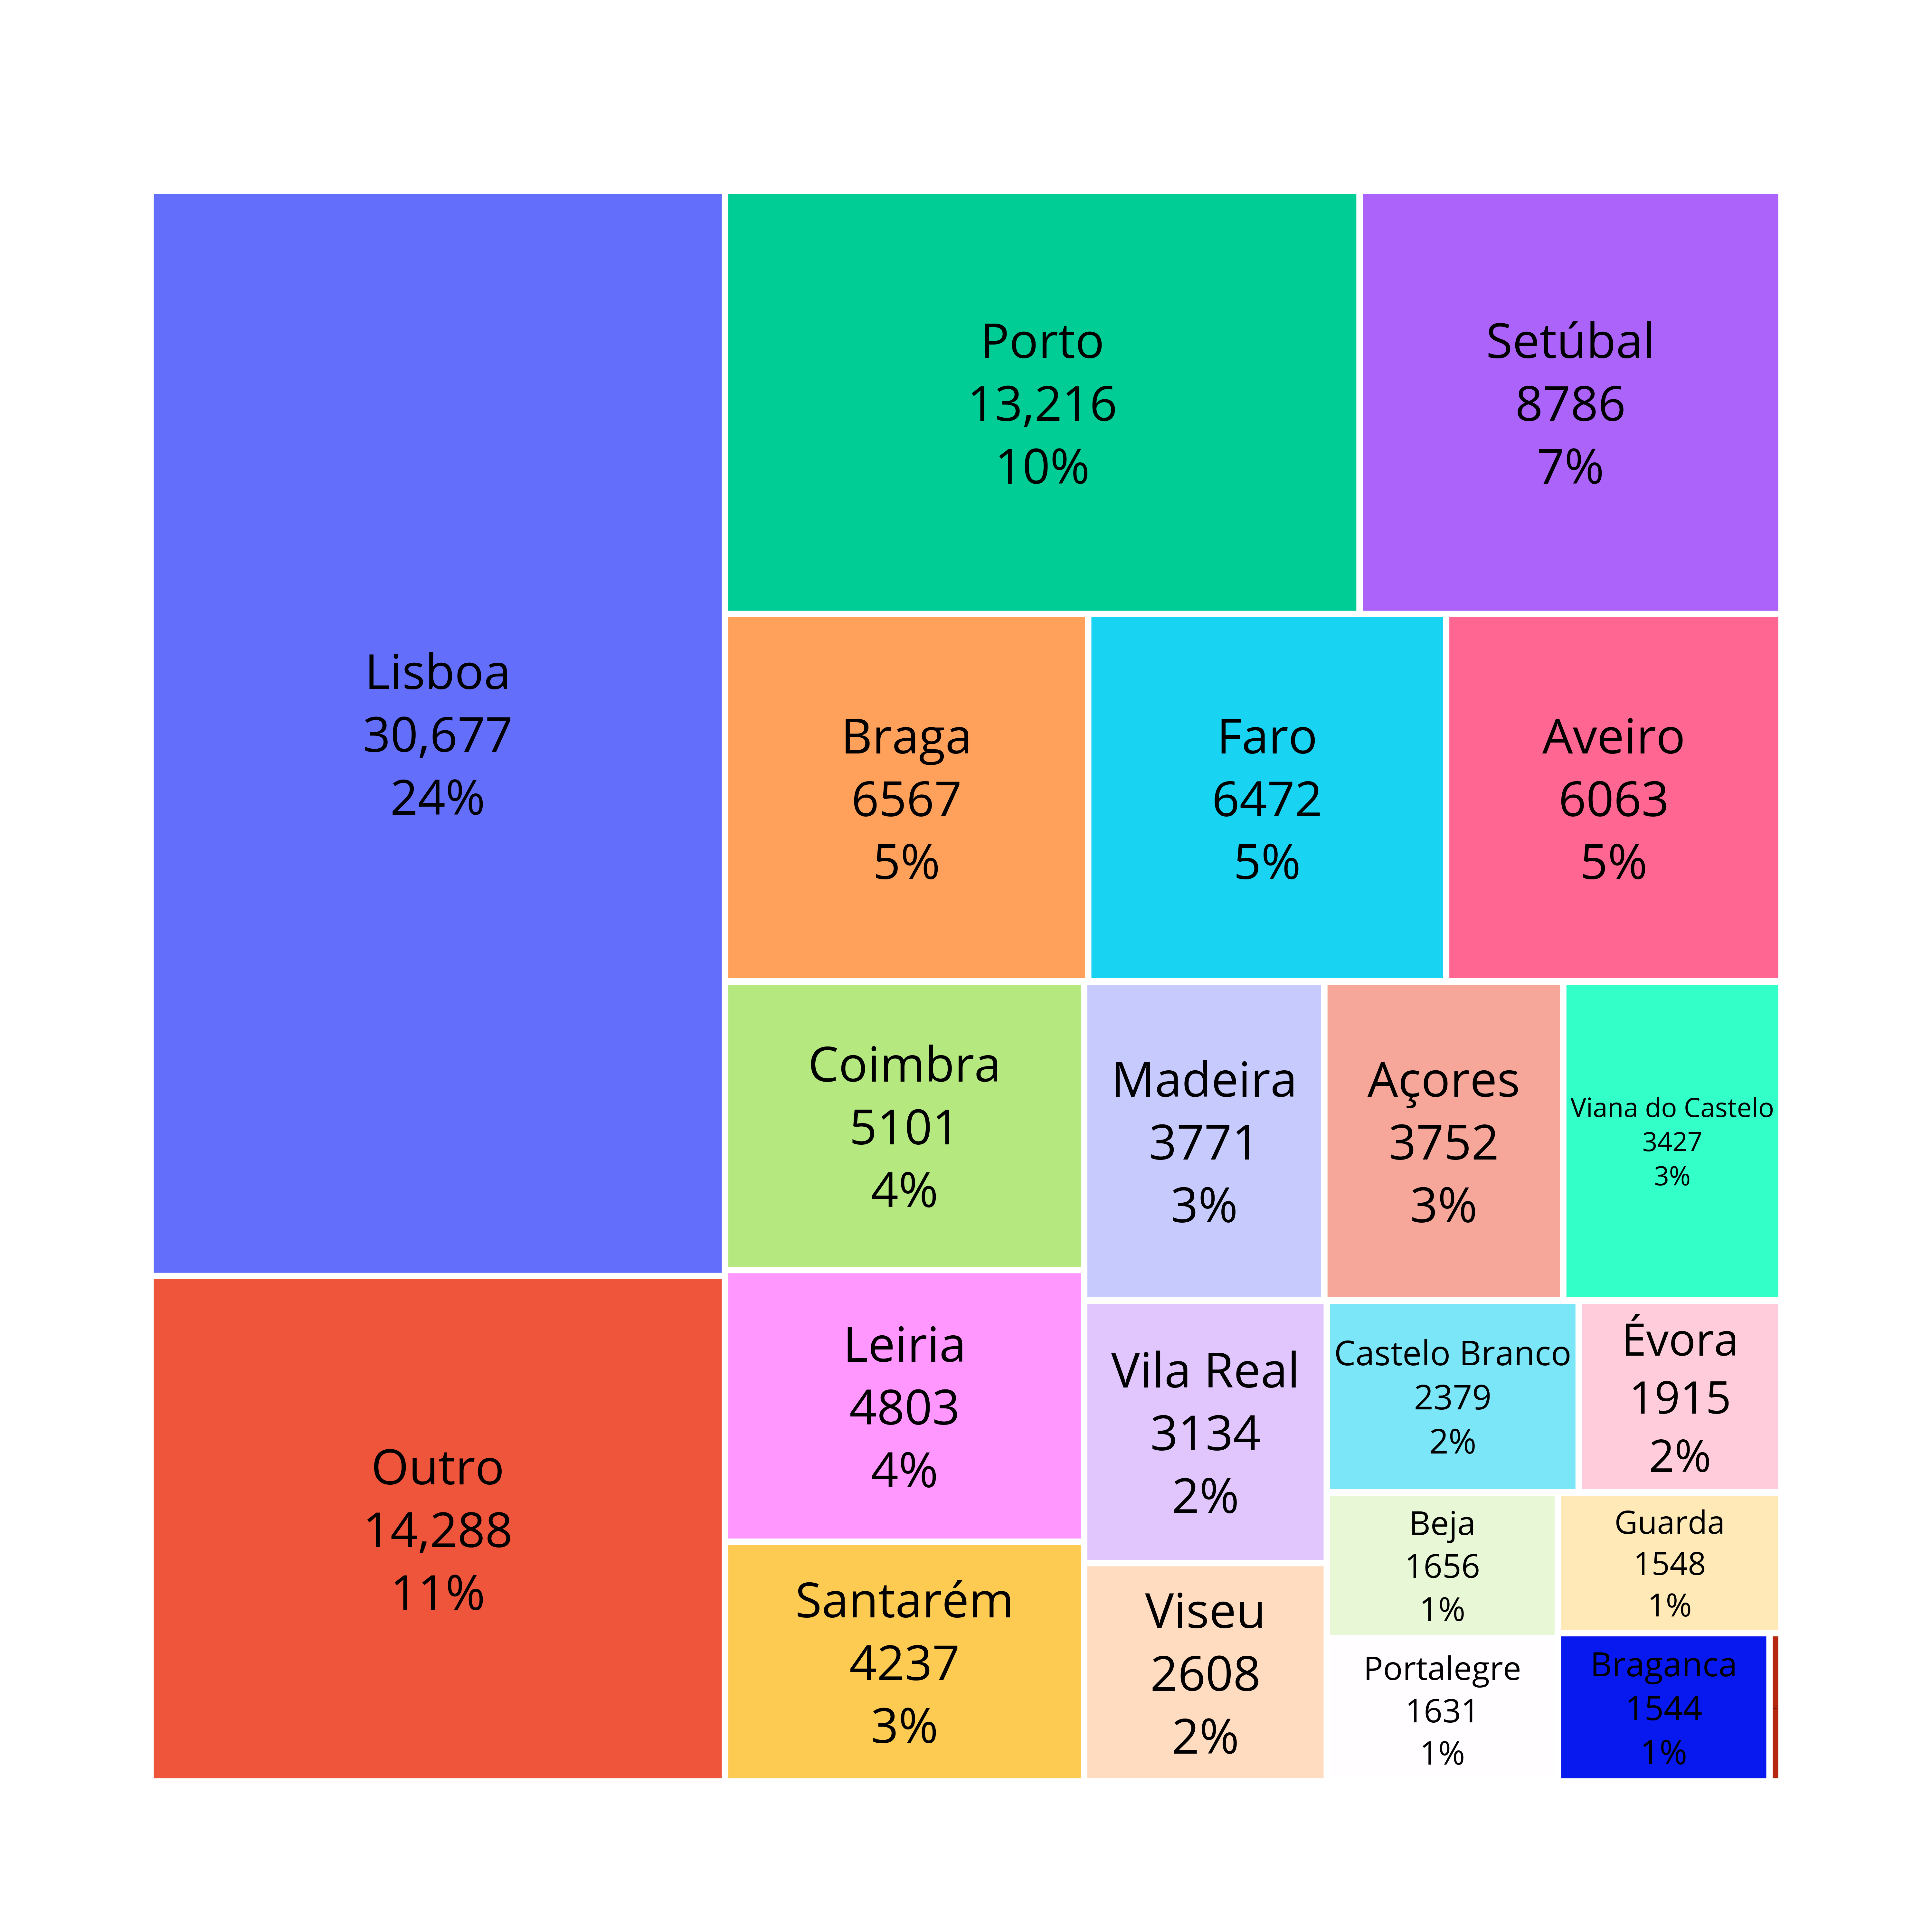
\includegraphics[width=\textwidth]{imagens/treemap_cpub_distritos.png}
		\caption{Distribuição do número de concursos públicos, por distrito.}
		\label{fig:cploc}
	\end{minipage}
	
	\vspace{1em}
	
	\begin{minipage}[t]{0.49\textwidth}
		\centering
		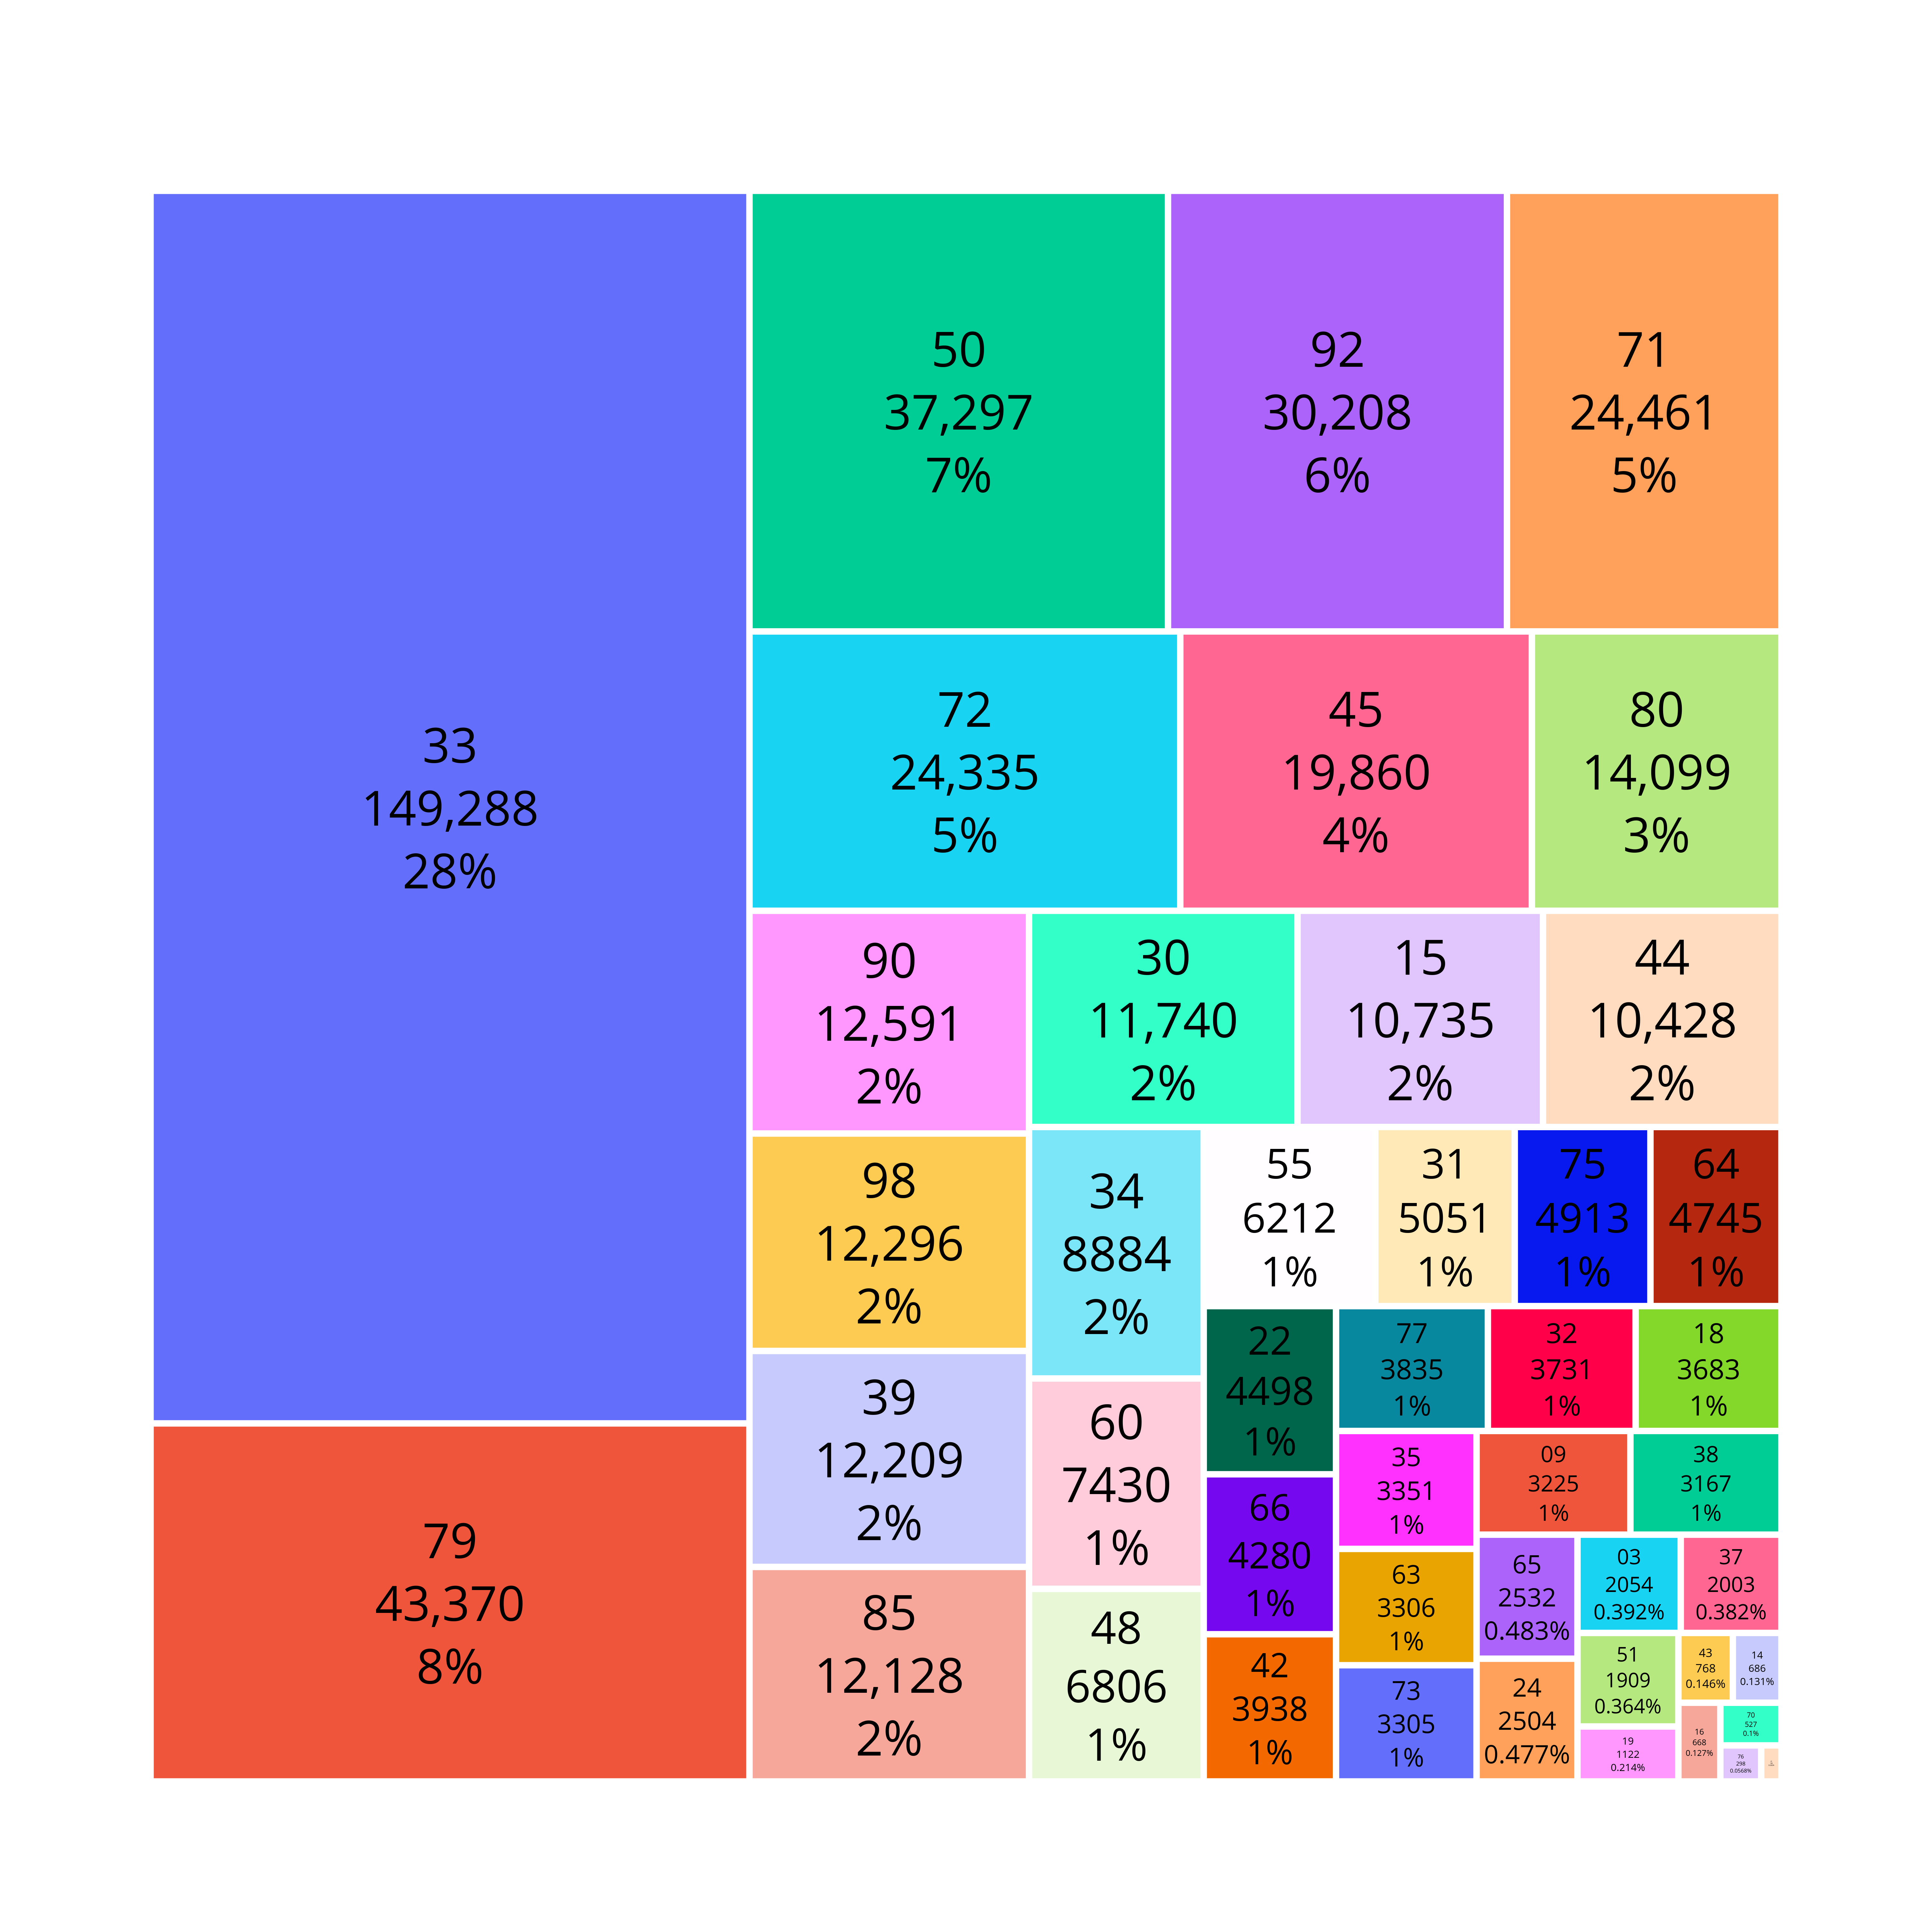
\includegraphics[width=\textwidth]{imagens/treemap_contratos_adir.png}
		\caption{Distribuição do número de ajustes diretos em regime geral, por divisão de CPV.}
		\label{fig:adcpv}
	\end{minipage}
	\hfill
	\begin{minipage}[t]{0.49\textwidth}
		\centering
		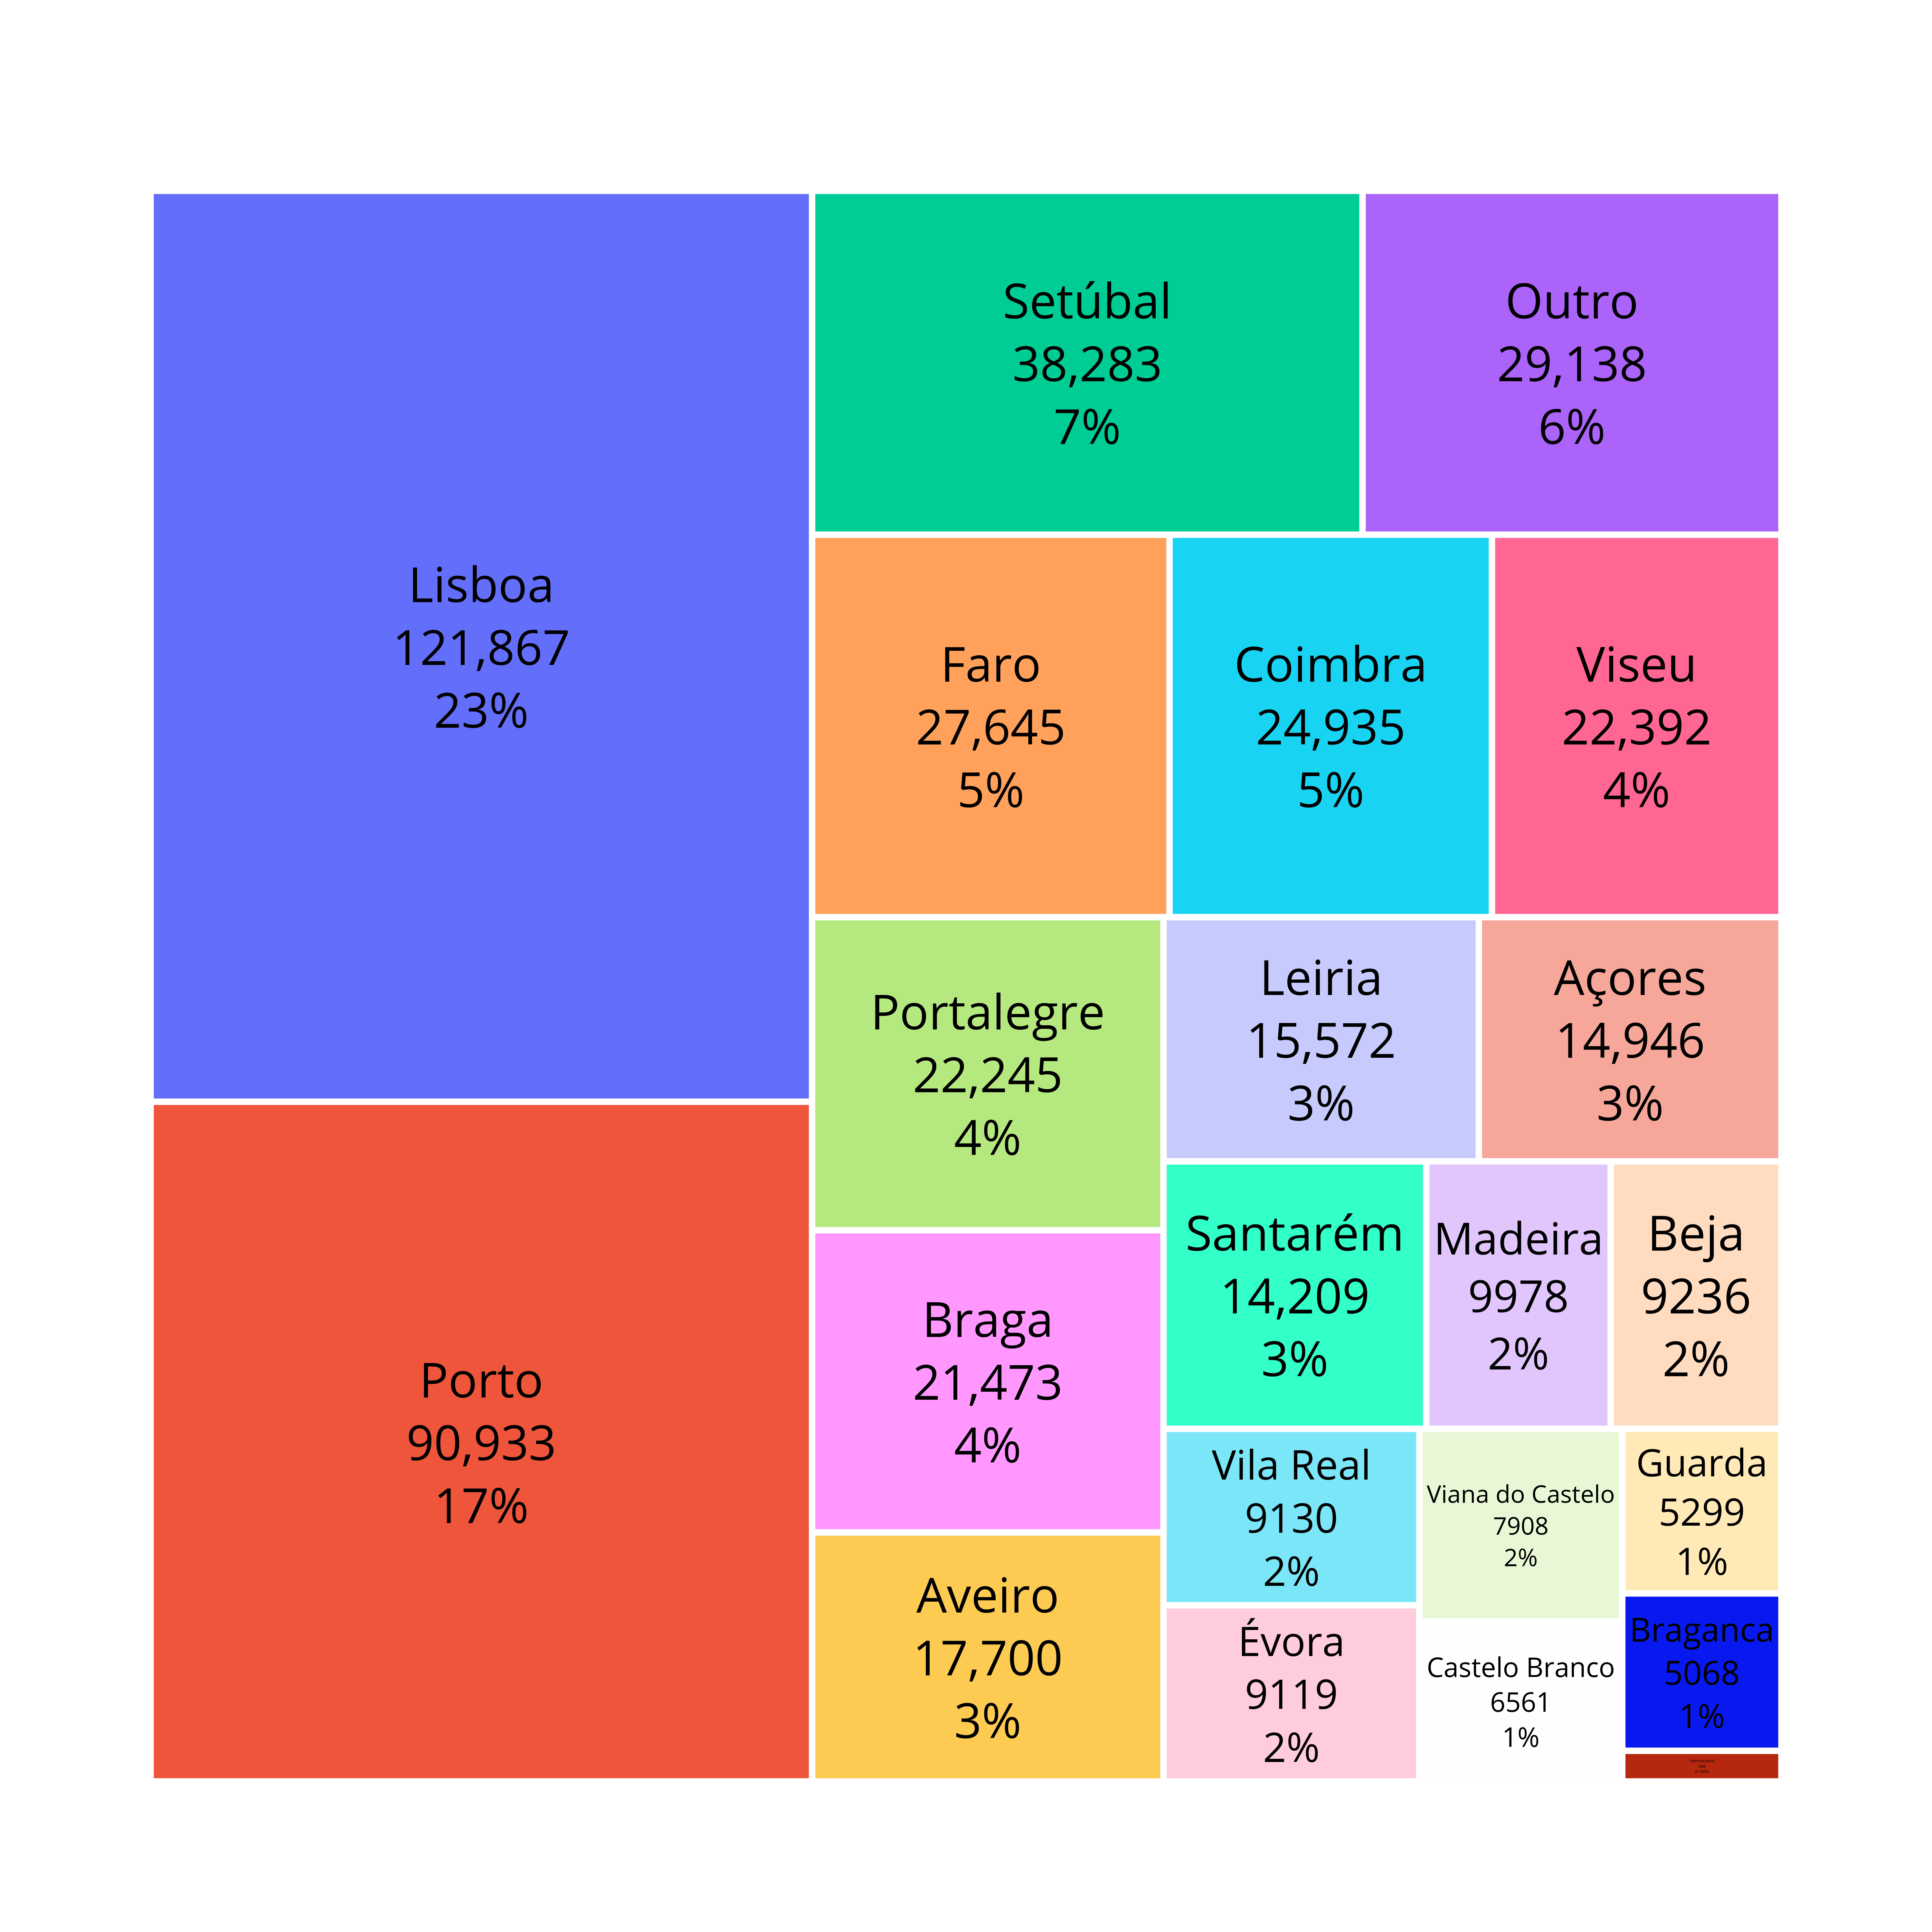
\includegraphics[width=\textwidth]{imagens/treemap_distritos_adir.png}
		\caption{Distribuição do número de ajustes diretos em regime geral, por distrito.}
		\label{fig:adloc}
	\end{minipage}
	
\end{figure}
\clearpage


%\subsection{Exemplo ilustrativo: Contratos referentes à área da saúde}
%
%\begin{figure}[H]
%	\begin{minipage}{0.33\linewidth}
%		%\centering  % redundant
%		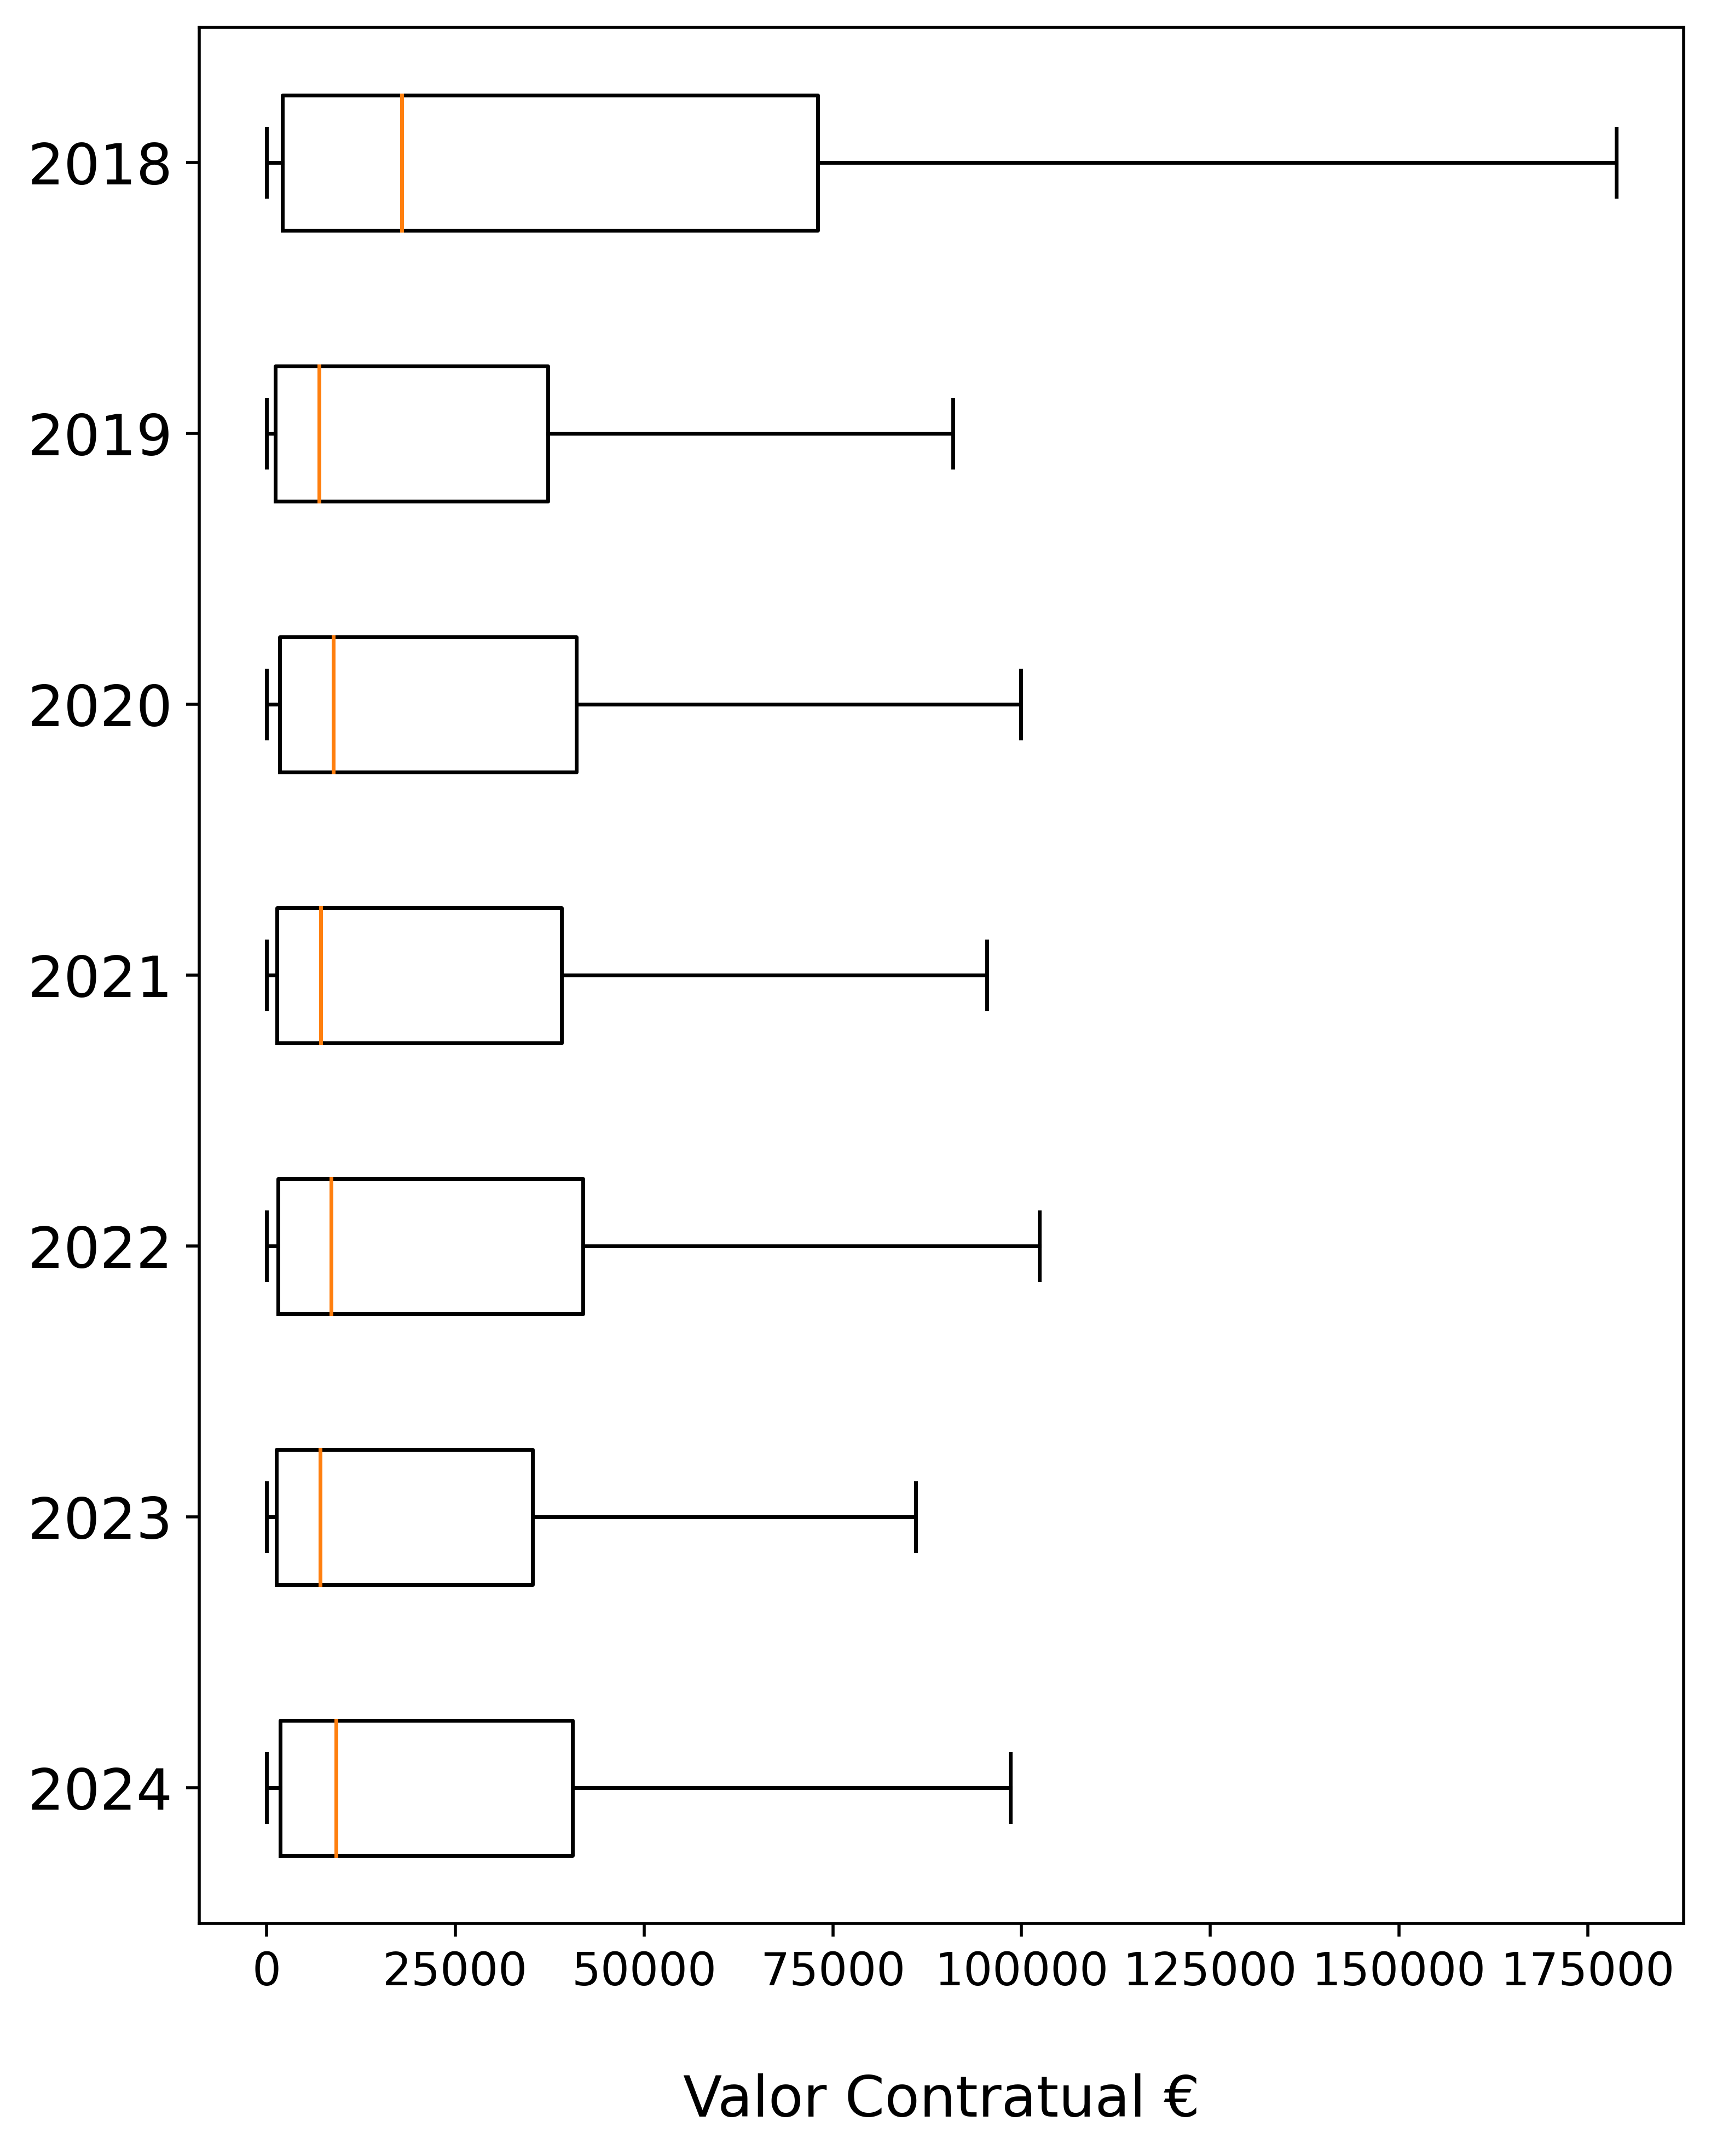
\includegraphics[width=\textwidth]{imagens/cp_anos_33_v1.png}
%		\caption{Boxplot dos preços contratuais para concursos públicos referentes à área da saúde desde 2018 até 2024}
%	\end{minipage}%
%	\hfill% not: "\hspace{0.5cm}"
%	\begin{minipage}{0.33\linewidth}
%		%\centering  % redundant
%		\includegraphics[width=\textwidth]{imagens/cp_anos_33_v2.png}
%		\caption{Número de concursos públicos celebrados referentes à área da saúde desde 2018 até 2024}
%	\end{minipage}%
%	\hfill% not: "\hspace{0.5cm}"
%	\begin{minipage}{0.33\linewidth}
%		%\centering  % redundant
%		\includegraphics[width=\textwidth]{imagens/cp_anos_33_v3.png}
%		\caption{Montante total adjudicada a contratos públicos celebrados referentes à área da saúde desde 2018 até 2024}
%	\end{minipage}
%\end{figure}
%
%
%
%\begin{figure}[H]
%	\begin{minipage}{0.33\linewidth}
%		%\centering  % redundant
%		\includegraphics[width=\textwidth]{imagens/ajdir_anos33_v1.png}
%		\caption{Boxplot dos preços contratuais para ajustes diretos em regime geral referentes à área da saúde desde 2018 até 2024}
%	\end{minipage}%
%	\hfill% not: "\hspace{0.5cm}"
%	\begin{minipage}{0.33\linewidth}
%		%\centering  % redundant
%		\includegraphics[width=\textwidth]{imagens/ajdir_anos33_v2.png}
%		\caption{Número de ajustes diretos em regime geral celebrados referentes à área da saúde desde 2018 até 2024}
%	\end{minipage}%
%	\hfill% not: "\hspace{0.5cm}"
%	\begin{minipage}{0.33\linewidth}
%		%\centering  % redundant
%		\includegraphics[width=\textwidth]{imagens/ajdir_anos33_v3.png}
%		\caption{Montante total adjudicada a ajustes diretos em regime geral celebrados referentes à área da saúde desde 2018 até 2024}
%	\end{minipage}
%\end{figure}

%
%
%
%\chapter{Noções Matemáticas}
%%\section{Indicadores Estatísticos Descritivos}
%
%Falar nesta secçaõ sobre:
%
%\begin{itemize}
%	\item Boxplot / diagrama de extremos e quartis
%	\item qunatis e as várias definições
%	\item outliers
%	\item função inversa generalizada
%	\item missing values
%	\item medidas de risco
%\end{itemize}
%
%
%\begin{figure}[H]
%	\centering
%	\includegraphics[width=0.7\textwidth]{imagens/skewed.png}
%	\caption{}
%	\label{}
%\end{figure}
%
%FAZER REPRESENTACAO GRÁFICA DESTE TIPO PARA JUSTIFICAR O PARÁGRAFO QUE ANTECEDE O PLOT DA COMPARACAO DA MEDIA, MEDIANA E DP DO NEC POR CPV DA FLAG R019

Um boxplot, também conhecido como diagrama de extremos e quartis, é uma ferramenta gráfica usada em Estatística para visualizar a distribuição de um conjunto de dados \cite{casella2002statistical} \cite{ross2014introduction}. A informação fornecida pelo boxplot é feita através dos seus componentes: 

\begin{my_itemize}
	
	\item Quartis: Os quartis são os valores que dividem um conjunto de dados ordenados em quatro partes iguais, cada uma contendo 25\% dos dados. Para calculá-los, é necessário organizar os dados por ordem crescente.O primeiro quartil (Q1), também conhecido como quartil inferior, é o valor abaixo do qual se encontram 25\% dos dados ordenados. O segundo quartil (Q2), ou mediana, é o valor abaixo do qual se encontra 50\% dos dados ordenados. O terceiro quartil (Q3), conhecido como quartil superior, é o valor abaixo do qual se encontra 75\% dos dados ordenados.
	
	\item Caixa: Representa o intervalo interquartil (IQR). Neste intervalo estão contidos  todos os dados cujo valor é superior ao primeiro quartil (Q1) e inferior ao terceito quartil (Q3), contemplando 50\% dos dados. A caixa permite verificar a dispersão dos dados: uma caixa maior indica uma maior variabilidade dos dados, enquanto que uma caixa menor indica uma menor variabilidade dos dados. 
	
	\item Mediana: É a linha que se encontra dentro da caixa e é apelidade de mediana (Q2). Esta linha divide o conjunto de dados em duas metadas iguais. É a partir da localização da mediana dentro da caixa que se pode observar a presença, ou não, de assimetria na distribuição dos dados. Se a linha se encontrar no meio, ou muito perto do meio, da caixa significa que a distribuição dos dados é simétrica. Por outro lado, se esta estiver deslocada para um dos lados significa que o conjunto de dados é assimétrico. 
	
	\item Extremidades (Whiskers): São as linhas que se estendem desde os primeiro e terceiro quartil até os valores mais extremos do conjunto de dados que não sejam considerados outliers. Existem diferentes formas de definir estas extremidadas\cite{spe},  mas, geralmente, são definidos como: $[Q1 - 1.5IQR, Q3 + IQR]$. As extremidades também permitem verificar a variabilidade dos dados. 
	
	\item Outliers: São todos os pontos que não são abrangidos pelas extremidades. São valores bastante diferentes dos demais e são representados por pontos individuais. A existência de um elevado número de outliers pode indicar a presença de distribuições com caudas longas e a presença de valores extremos.
	
\end{my_itemize}


Os boxplots permitem ter uma visão da distribuição dos dados, identificando rapidamente outliers e assimetrias para uma amostra com um número de observações estatisticamente significativo. Contudo, não detalha a distribuição de uma forma completa e, por isso, é frequentemete acompanhado de um histograma.



\begin{figure}[H]
	\centering
	\includegraphics[width=\textwidth]{imagens/stats/hist2.png}
	\caption{Exemplo de ilustração de histograma e boxplot para diferentes distribuições.}
	\label{fig:histos}
\end{figure}


Na Figura \ref{fig:histos} podem ser observadas três cenários distintos. Cada uma das amostras é composta por 1000 pontos gerados a partir das bibliotecas Numpy e Scipy do Python \cite{python}. A primeira amostra foi gerada a partir de uma distribuição normal com valor médio 0 e uma variância de 0.5, a segunda a partir de uma distribuição normal com valor médio 0 e variância 1 e a terceira a partir de uma distribuição normal assimétrica, usando o módulo scipy.stats.skewnorm. A partir da observação dos dois primeiros gráficos, verifica-se que a distância interquartil do primeiro é inferior à do segundo, resultado de uma menor variância/ maior concentração dos dados. No terceiro gráfico encontra-se uma distribuição assimétrica à esquerda. Através do seu boxplot, verifica-se que os whsikers não têm o mesmo tamanho e a mediana encontra-se mais próxima do primeiro quartil do que do terceiro. 


\section{Outliers}


























%
%
%
%\chapter{Construção das \textit{Red Flags}}
%%\section{Exploração do Dataset}
%
%Numa primeira fase foram criadas funções para explorar o conjunto de dados. \\
%
%A função \textbf{col\_names} retorna-nos uma dataframe com todos os nomes das colunas. A função \textbf{n\_contracts} retorna-nos o número de linhas, ou seja, o número de contratos totais, da base de dados. \\
%
%Foi desenvolvida, também, uma função \textbf{h} que permite ver uma dataframe de forma mais apresentável.\\
%
%\textit{É preciso criar uma função com o código que já tenho para categorizar os contratos de acordo com o tipo de procedimento. Idem para o tipo de contrato.} \\

 

%\begin{table}[H]
%	\centering
%	\includegraphics[width= \textwidth]{tabelas/tabela_rf.pdf}
%	\caption{}
%	\label{}
%\end{table}



 

%\section{Funções Auxiliares}
%
%Para a construção das \textit{flags} são necessárias outras funções mais simples. Certas funções irão ter um único propósito e os outputs de certas funções irão ser usados como inputs de outras funções. \\
%
%Para identificar um contrato necessitamos do seu id. Assim, criou-se uma função \textbf{all\_ids} que retorna os ids de todos os contratos da base de dados. Contudo, como não vamos trabalhar com todos os tipos de contratos e procedimentos, é necessário filtrar estes ids.
%Para tal, criaram-se as funções \textbf{ajustes\_dir}, \textbf{consulta\_prev} e \textbf{concurso\_pub} que retornam os ids de todos os ajustes diretos, consultas prévias e concursos públicos, respetivamente. \\
%
%De seguida, filtraram-se os contratos por tipo de procedimento e por CPV. Para isso, criou-se a função \textit{cpv\_direto} que retorna todos os ids de ajustes diretos para serviços de consultoria em IT ( todos os CPV's começados por 72). De seguida, foi feito o mesmo para contratos públicos na função \textit{cpv\_cpub}. De forma a generalizar, criou-se a função \textit{cpv} que retorna todos os ids de contratos de um tipo de procedimento e para um determinado CPV. Tanto o tipo de procedimento como os primeiros 2 algarismos do CPV são parâmetros de entrada da função. \\
%
%
%Para começar, criaram-se duas funções que permitem ver qual é o contrato associado a um determinado id. A função \textit{contrato} tem como input um único id de um contrato ( todas estas funções dizem respeito à tabela \textit{contratos} da DB) e retorna uma dataframe com uma única linha referente ao contrato associado a esse mesmo id. A função \textit{contratos} faz exatamente a mesma coisa mas para um conjunto de id's. \\
%
%Quando as flags estiverem construídas e quisermos ver o anúncio de um contrato suspeito no site do basegov, podemos fazê-lo usando a função \textit{url} que, novamente, tem como parâmetro de entrada o id de um contrato. Esta função pode ter bastante utilidade nos casos que chamam bastante a atenção, como por exemplo, quando se viu um ajuste direto de 3 milhões de euros. \\



\section{Contratação Fechada}

\subsection{RF1 : Verificação dos Preços Contratuais para Ajustes Diretos em Regime Geral}


Como foi apresentado anteriormente na tabela 1.4, os ajustes diretos tem diferentes limites máximos impostos por lei, mediante o tipo de obra/serviço. 
A fim de poder identificar os contratos que não estão em conformidade com o CCP, foi necessário fazer algumas alterações na base de dados. Primeiro, foi necessário classificar o ajuste direto de acordo com o critério. Se os critério for Critério do Valor, os valores máximos permitidos são os que se encontram presentes na tabela 1.4. Se o critério for Critério Material, estamos perante uma situação em que pode ser adotado o ajuste direto independentemente do valor do contrato a celebrar. Assim, a partir da coluna \textit{fundamentacao} da tabela, pode-se verificar qual o artigo do CCP adotado para realizar o ajuste direto. 


\begin{table}[H]
	\centering
	\begin{tabular}{|c|c|c|c|}
		\hline
		\textbf{Critério}                  & \textbf{Artigos}           & \textbf{Tipo de Contrato}           & \textbf{Valor} \\ \hline
		\multirow{3}{*}{Critério do Valor} & \multirow{3}{*}{17º a 22º} & Aquisição de bens móveis e serviços & 20000€         \\ \cline{3-4} 
		&                            & Empreitadas de obras públicas       & 30000 €        \\ \cline{3-4} 
		&                            & Outro tipo de contratos             & 50000 €        \\ \hline
		Critério Material                  & 24º a 27º                  & Qualquer                            & Indefinido     \\ \hline
	\end{tabular}
	\caption{text}
\end{table}

Assim, foi criada uma nova coluna \textit{artigo} que, a partir da coluna \textit{fundamentacao}, guarda apenas o artigo presente - ignora as alíneas. 

\begin{lstlisting}[
	language=SQL,
	showspaces=false,
	showstringspaces=false,
	basicstyle=\ttfamily,
	numbers=left,
	numberstyle=\tiny,
	commentstyle=\color{gray}, frame = single,	autogobble=true,
	postbreak=\mbox{\textcolor{red}{$\hookrightarrow$}\space},
	]
	ALTER TABLE ajustesdiretos
	ADD COLUMN artigo text;
	
	UPDATE ajustesdiretos
	SET artigo = TRIM(SUBSTRING(fundamentacao 
			FROM 1 FOR POSITION('º' IN fundamentacao)));
\end{lstlisting}





De seguida, foi criada uma coluna \textit{criterio}, constituída apenas por duas strings : valor e material. Para um determinado contrato, se o artigo no campo \textit{fundamentacao} pertencer entre o 17º e o 22º, então é-lhe atribuído o critério valor. Caso contrário, o cirtério material. 


\begin{lstlisting}[
	language=SQL,
	showspaces=false,
	showstringspaces=false,
	basicstyle=\ttfamily,
	numbers=left,
	numberstyle=\tiny,
	commentstyle=\color{gray}, frame = single,	autogobble=true,
	postbreak=\mbox{\textcolor{red}{$\hookrightarrow$}\space},
	]
	ALTER TABLE ajustesdiretos
	ADD COLUMN criterio text;
	
	UPDATE ajustesdiretos
	SET criterio = CASE
	WHEN artigo = 'Artigo 17.º' OR artigo = 'Artigo 18.º' 
	OR artigo = 'Artigo 19.º' OR artigo = 'Artigo 20.º' 
	OR artigo = 'Artigo 21.º' OR artigo = 'Artigo 22.º' 
	THEN 'valor'
	
	ELSE 'material' 
	END;
\end{lstlisting}


Assim, é possível identificar todos os contratos que não respeitem os valores apresentados nas tabelas 1.4 e 4.1 através das seguintes \textit{queries} : 

\begin{lstlisting}[
	language=SQL,
	showspaces=false,
	showstringspaces=false,
	basicstyle=\ttfamily,
	numbers=left,
	numberstyle=\tiny,
	commentstyle=\color{gray}, frame = single,	autogobble=true,
	breaklines=true,
	postbreak=\mbox{\textcolor{red}{$\hookrightarrow$}\space},
	]
	SELECT * FROM ajustesdiretos
	WHERE criterio = 'valor' AND tipocontrato = 'Bens e Servicos' AND preco > 20000;
	
	SELECT * FROM ajustesdiretos
	WHERE criterio = 'valor' AND 
	tipocontrato = 'Empreitadas' AND preco > 30000;
\end{lstlisting}




%Esta função tem como input uma dataframe correspondente a todos os ajustes diretos realizados com CPV 72, sendo esta obtida fazendo uso dos funções \textit{contratos} e \textit{cpv} definidas antes, e os ids dos contratos associados aos ajustes diretos. 
%A função vai comparar todos os preços contratuais com o valor de 20.000€ pois é o limite máximo de aquisição de serviços. Esta parte tem de  ser atualizada no futuro. Contudo, a maior parte dos ajustes diretos é Aquisição de Serviços. Se os valores forem superiores a este preço, é ativada uma flag.
%A segunda parte da função verifica se foi feita uma fundamentação para o ajuste direto. Esta vai ser sempre uma alínea qq do CCP. Mas tem de estar preenchida. Se o valor ultrapassar os 20000€ e não estiver fundamentado é claramente comportamento suspeito. Se o contrato só tiver a parte da fundamentação por preencher, pode ser má prática. 








\section{Contratação Aberta}

\subsection{R003 : Análise do Prazo de Apresentação de Propostas}


\Lemma{}
{
	Short or inadequate notice to bidders to submit expressions of interest or bids. Bid period is less than expected (usually <=2 days)
	The indicator should be calculated grouping by procurement method used, since the minimum bidding period might vary depedning on the method.  It is important to check in local regulations if there is a minimun period.  
}


De acordo com o artigo 135.º do CCP, o prazo mínimo para apresentação de propostas num concurso público não pode ser inferior a 6 dias e, no caso de se tratar de um procedimento de formação de um contrato de empreitada de obras públicas, a 14 dias. Assim, foi criada uma coluna adicional, \textit{tipocontrato}, para a criação desta flag a partir da coluna \textbf{contratCtypes}. Sempre que, para um determinado contrato, o tipo de contrato contiver a palavra Empreitada, é atribuída a string \textit{Empreitada} à nova coluna. Caso contrário, é atribuída a string \textit{Bens e Serviços}. De seguida, foi construída uma \textit{query} em PostgreSQL para determinar todos os contratos referentes a concursos públicos que não respeitam estas condições. \\


\begin{lstlisting}[
	language=SQL,
	showspaces=false,
	showstringspaces=false,
	basicstyle=\ttfamily,
	numbers=left,
	numberstyle=\tiny,
	commentstyle=\color{gray}, frame = single,
	autogobble=true,
	breaklines=true,
	postbreak=\mbox{\textcolor{red}{$\hookrightarrow$}\space},
	]
	SELECT concursospublicos."id"
	FROM concursospublicos
	WHERE tipocontrato = 'Empreitadas' AND prazo_execucao < 14;
	
	SELECT concursospublicos."id"
	FROM concursospublicos
	WHERE tipocontrato = 'Outro' AND prazo_execucao < 6;
	
\end{lstlisting}


No código acima, \textit{concursospublicos} diz respeito à tabela da base de dados que contém a totalidade de concursos públicos obtidos através da plataforma BaseGov. Ambas as \textit{queries} devolvem os ids dos contratos celebrados que não estão em conformidade com o CCP. 




\subsection{R017 : Comparação do Preço Contratual com Preço Médio por CPV}


\Lemma{}
{
	The difference between an item value and its expected value is above a threshold. 
}

Para construção deste indicador foi calculado o preço médio por CPV. O conjunto de contratos foi agrupado pelos primeiros três dígitos - grupo - do CPV de forma a obter um maior nível de granularidade. Para cada um dos 302 grupos foi calculado o preço contratual médio, desvio padrão, mínimo, máximo e primeiro, segundo e terceiro quartis. O resultado obtido assemelha-se à seguinte tabela : 


\begin{table}[h!]
	
	\setlength\tabcolsep{1pt}
	\begin{tabular*}{\linewidth}{@{\extracolsep{\fill}} |c|c|c|c|c|c|c|c|c|c|}
		\hline
		\textbf{cpv3} & \textbf{preco\_total} & \textbf{count} & \textbf{mean} & \textbf{std} & \textbf{min} & \textbf{q1} & \textbf{q2} & \textbf{q3} & \textbf{max} \\ \hline
		641           & 6700942.8           & 57             & 117560.4    & 179755.1   & 1575         & 10639.2     & 60000       & 165892.2    & 885500       \\ \hline
	\end{tabular*}
	\caption{Primeira linha da tabela auxiliar construída}
	
\end{table}


Contudo, a partir da construção desta tabela, constatou-se que, certamente devido a erros de preenchimento na plataforma BaseGOV, existem inúmeros valores de preço contratuais com valores negativos ou com valor nulo. Desta forma, o valor médio calculado não corresponde ao verdadeiro valor médio e, como tal, a comparação que se pretendia efetuar na próxima etapa deste indicador entre o preço contratual e o preço médio contratual por grupo é inapropriada. 

\subsection{R018 : Análise de Contratos com uma entidade concorrente}


\Lemma{}
{
	Single bid received : Tender featured a single bidder only 
}


Dado que uma das colunas da tabela diz respeito às entidades concorrentes, pode ser feita uma análise do número de entidades que concorrem a um determinado concurso. De acordo com a diretriz da OCDS, esta flag é ativada em situações em que haja apenas uma entidade a candidatar-se a um concurso. 

Para tal, foi preciso criar uma nova coluna \textit{nr\_entidadesconcorrentes} que contenha apenas o número de entidades concorrentes. Visto que a coluna \textit{entidades\_concorrentes} contém elementos da forma :



\begin{table}[H]
	\centering
	\begin{tabular}{|c|c|}
		\hline
		\textbf{ID}   & \textbf{EntidadesConcorrentes}                                                                                                      \\ \hline
		$\text{ID}_1$ & $\text{Entidade}\_i$ ( $\text{NIF}\_i$) $|||$ $\text{Entidade}\_j$ ( $\text{NIF}\_j$)                                               \\ \hline
		$\text{ID}_2$ & $\text{Entidade}\_k$ ( $\text{NIF}\_k$)                                                                                             \\ \hline
		$\dots$       & $\dots$                                                                                                                             \\ \hline
		$\text{ID}_n$ & $\text{Entidade}\_l$ ( $\text{NIF}\_l$) $|||$ $\text{Entidade}\_m$ ( $\text{NIF}\_m$) $|||$ $\text{Entidade}\_n$ ( $\text{NIF}\_n$) \\ \hline
	\end{tabular}
	\caption{Formato da coluna EntidadesConcorrentes}
\end{table}

foi necessário desenvolver uma \textit{query} que, para cada elemento da coluna \textit{entidades\_concorrentes}, os separe de cada vez que encontra o separador $|||$ e conte o número de entidades total. Esse número, por conseguinte, é alocado para a nova coluna criada. 


\begin{lstlisting}[
	language=SQL,
	showspaces=false,
	basicstyle=\ttfamily,
	numbers=left,
	numberstyle=\tiny,
	commentstyle=\color{gray}, frame = single,
	breaklines=true,
	autogobble =true,
	postbreak=\mbox{\textcolor{red}{$\hookrightarrow$}\space},
	]
	UPDATE concursospublicos
	SET nr_entidadesconcorrentes = ARRAY_LENGTH(STRING_TO_ARRAY( entidades_concorrentes, '|||'), 1) + 1;	
\end{lstlisting}



\begin{figure}[H]
	\centering
	\includegraphics[width=\textwidth]{imagens/r018.png}
	\caption{Grupos com maior número de contratos indiciados}
	\label{}
\end{figure}

\subsection{R019 : Análise do Número de Entidades Concorrentes}

\Lemma{}
	{
	Low number of bidders for item and procuring entity. Number of bidders significantly less than average, based on prior similar contracts (for similar item or procuring entity) 
	}


Para a construção deste indicador, foi necessário construir uma tabela adicional. Para cada uma das 46 divisões de CPV, foi feita uma contagem de todos os contratos, calculado o número total de entidades concorrentes de entre todos os contratos e foram calculados os seguintes indicadores estatísticos : média, desvio-padrão, primeiro-quartil, segundo-quartil, terceiro-quartil, mínimo e máximo. Este procedimento foi feito através de um script \textit{python}, obtendo-se uma tabela do género : 

\begin{table}[H]
	\centering
	\begin{tabular}{|c|c|c|c|c|c|c|c|c|c|}
		\hline
		\textbf{cpv} & \textbf{nec\_t} & \textbf{count} & \textbf{mean} & \textbf{std} & \textbf{min} & \textbf{q1} & \textbf{q2} & \textbf{q3} & \textbf{max} \\ \hline
		98           & 1739            & 586            & 2.968         & 2.251        & 1            & 1           & 2           & 4           & 15           \\ \hline
	\end{tabular}
	\caption{}
\end{table}

sendo que \textbf{cpv} corresponde a cada umas das divisões de CPV, \textit{nec\_t} corresponde ao número total de entidades concorrentes em todos os concursos, \textit{count} é número total de contratos, \textbf{mean}, \textbf{std}, \textbf{min}, \textbf{q1}, \textbf{q2}, \textbf{q3} e \textbf{max} são, respetivamente, o valor médio, o desvio padrão, mínimo, primeiro quartil, segundo quartil, terceiro quartil e máximo para todos os contratos cujos primeiros dois digitos do CPV sejam iguais aos da primeira coluna. 

Com o resultado obtido, foi feita, numa primeira instância, uma representação gráfica dos valores da média, mediana e desvio-padrão, por CPV, a fim de ter uma ideia da dispersão - distância entre a média e o desvio padrão - e simetria da distribuição - distância entre média e mediana - dos preços contratuais.

\begin{figure}[!htbp]
	\centering
	\includegraphics[width=\textwidth]{imagens/mmdp.png}
	\caption{Comparação da Média, Mediana e Desvio Padrão do NEC em CP por CPV}
	\label{}
\end{figure}

Foi, também, feita uma representação gráfica do boxplot para cada umas divisões do CPV. 

\begin{figure}[!htbp]
	\centering
	\includegraphics[width=.9\textwidth]{imagens/cpv1.png}
	\caption{Boxplot referente ao número de entidades concorrentes em Concursos Públicos por CPV : I}
	\label{}
\end{figure}


\begin{figure}[h!]
	\centering
	\includegraphics[width=.9\textwidth]{imagens/cpv2.png}
	\caption{Boxplot referente ao número de entidades concorrentes em Concursos Públicos por CPV : II}
	\label{}
\end{figure}


Assim, a fim de selecionarmos os IDs de todos os contratos que respeitem a definição enunciada anteriormente, foi construída a seguinte \textit{query} que retorna todos os contratos cujo número de entidades concorrentes seja inferior à metade do número de entidades concorrentes esperado.  

\begin{lstlisting}[
	language=SQL,
	showspaces=false,
	basicstyle=\ttfamily,
	numbers=left,
	numberstyle=\tiny,
	commentstyle=\color{gray}, frame = single,
	breaklines=true,
	autogobble =true,
	postbreak=\mbox{\textcolor{red}{$\hookrightarrow$}\space},
	]
	SELECT concursospublicos."id"
	FROM concursospublicos 
	JOIN cpv_stat ON concursospublicos."cpv2" = cpv_stat."cpv"
	WHERE concursospublicos."nr_entidadesconcorrentes" < 0.5 * cpv_stat."mean";
\end{lstlisting}

Os resultados obtidos, que podem ser observados na seguinte figura, mostram que existe uma forte predominância dos CPVs começados por 33 e 45, o que pode ser um indicador de que existe um elevado número de contratos com um número \textit{baixo} de entidades concorrentes. 

\begin{figure}[H]
	\centering
	\includegraphics[width=\textwidth]{imagens/r019.png}
	\caption{Grupos com maior número de contratos indiciados}
	\label{}
\end{figure}





\subsection{R031 : Análise da relação entre Preço Base e Preço contratual}

A primeira flag construída tem como objetivo comparar o preço base com o preço contratual.


Numa primeira instância, pegou-se num \textit{subset} de contratos da base de dados em PostgreSQL e guardou-se numa \textit{dataframe} em Python. 
Utilizando a função \textit{cpv}, obtiveram-se os id's dos contratos de um dos tipos de contrato desejados e para um determinado cpv. Numa fase inicial optou-se pelos ids concursos públicos para CPV's começados por 72. 


Para se poder comparar ambos os preços foram desenvolvidas algumas funções auxiliares.
Primeiramente, desenvolveu-se a função \textit{preco\_contratual1} que devolve, a partir do id de um anúncio, o valor do preço contratual desse mesmo anúncio.
A função \textit{preco\_contratual2} faz o mesma coisa mas para um tabela genérica pertencente à base de dados. A função \textit{preco\_contrato3} generaliza a primeira função, pois retorna um conjunto de preços contratuais referentes a um conjunto de ids de anúncios que leva como input. A função \textit{preco\_contratual4} generaliza a função anterior para qualquer tabela. Os precos contratuais são retornados no formato de array.


De seguida, foi feito o mesmo para o preço base. Foi utilizada a mesma abordagem e construíu-se a função \textit{preco\_base3} que retorna os valores dos preços base para um conjunto de id's. 


Assim, foi construída uma primeira versão para esta flag. 

\begin{verbatim}
	def redflag(pbase, pcontr, tol, ids, r, df):
\end{verbatim}

Definiram-se como parâmetros de entrada desta função o conjunto de preços bases - pbase - e preços contratuais - pcontr - associados a um determinado conjunto de ids - ids - que já conseguimos determinar usando as funções criadas anteriormente. É preciso fornecer uma tolerância - tol - que vai definir a diferença máxima permitida entre o preço base e o contratual e um racio máximo permitido entre o preco base e contratual. 


O objetivo desta flag é identificar todos os contratos cujo preço contratual pertença a um intervalo em torno do preço base, definido pelo parâmetro \textit{tol}.

\begin{figure}[H]
	\centering
	\includegraphics[width=0.7\textwidth]{imagens/pbasecontr.png}
	\caption{}
	\label{}
\end{figure}


%O preço base é conhecido à priori, por isso esta flag não tem muito valor por si só. Quando for acoplada com outras flags pode sugerir um comportamento suspeito. Também é preciso ter em conta como é que o preço base é calculado. Se o preço base for calculado por excesso e o preço contratual for próximo do preço base, pode haver corrupção tanto por parte da entidade adjudicante como da adjudicatária. 

Contudo, ao longo da construção desta flag verificou-se a existência de casos em que o preço base é significativamente superior ao preço contratual, chegando a atingir uma ordem de grandeza de $\approx 10^2$. Isto deve-se a dois fatores : o preço base definido é demasiado elevado comparativamente ao preço contratual ou o preço base diz respeito a casos em que a adjudicação de um determinado serviço/obra é feita por lotes.

\begin{table}[H]
	\centering
	\begin{tabular}{|c|c|c|c|c|}
		\hline
		\multicolumn{1}{|l|}{\textbf{Número de Anúncio}} & \multicolumn{1}{l|}{\textbf{ID}} & \multicolumn{1}{l|}{\textbf{Lote}} & \multicolumn{1}{l|}{\textbf{Preço Base}} & \multicolumn{1}{l|}{\textbf{Preço Contratual}}          \\ \hline
		& 10471090                         & 1                                  &                                          & \cellcolor[HTML]{F2FCFE}{\color[HTML]{555555} 77454.72} \\ \cline{2-3} \cline{5-5} 
		& 10471049                         & 2                                  &                                          & \cellcolor[HTML]{F2FCFE}{\color[HTML]{555555} 85365.84} \\ \cline{2-3} \cline{5-5} 
		\multirow{-3}{*}{11171/2023}                     & 10470972                         & 3                                  & \multirow{-3}{*}{373860.48}              & \cellcolor[HTML]{F2FCFE}{\color[HTML]{555555} 89886.72} \\ \hline
	\end{tabular}
	\caption{Exemplo de contrato adjudicado por lotes}
\end{table}


Tendo em conta que na base de dados não é disponibilizado o preço base para cada lote, foi utilizada a seguinte abordagem. É de salientar que no caso de adjudicação por lotes, o número de anúncio é igual para cada um dos lotes, mas cada lote tem um id diferente. 

Sempre que o rácio $\text{preçobase} / \text{preçocontratual}$, para um certo contrato, é superior a determinado limite, o respetivo id é guardado. A partir do id do contrato obtém-se o número do anúncio e, para todos os contratos com o mesmo número de anúncio, são somados os preços contratuais e o resultado final é comparado com o preço base. 

Por fim, o resultado final é um conjunto de id's na forma de tuplo que respeita as condições anteriormente mencionadas.




%\section{Análise dos Concursos Públicos}
%
%Aqui só foram usadas funções ja definidas. Criaram-se variáveis que guardam o valor do preço base e contratual dos concursos. Deu-se isso como input à funcao \textit{redflag}, além dos outros que são definidos por mim, e obtiveram-se as redflags. Representou-se um barplot dos precos contratuais em cima dos preços base para verificar a diferença entre os mesmos. 


%\section{Análise dos Ajustes Diretos em Regime Geral}
%
%Aqui, novamente, foram utilizadas as funções já criadas anteriormente para obter uma dataframe com os contratos referentes a ajustes diretos e os ids associados. Foi feito um sumário estatístico dos valores dos preços contratuais e um histograma e um boxplot. Mas como tem outliers, vê-se mal. 
%Ordenei os ajustes diretos por fundamentação. Não nenhum campo vazio. 
%Com isto tudo ja se podem calcular as flags usando a função \textit{redflag2}. 
%É interessante saber qual a proporção de atividades suspeitas por entidade adjudicante e entidade adjudicatária. Para isso, calculou-se primeiro o número de contratos suspeitos e respetiva percentagem. 
%Para conseguir analisar foi preciso separar as colunas das entidades adjudicantes e adjudicatárias - que estavam no formato Entidade(NIF)(URL) - em três colunas distintas para cada uma das duas entidades. Isto é necessário para filtrar os contratos pelo NIF porque diferentes entidades podem ter o mesmo NIF. 
%Depois disso, ordenou-se por ordem decrescente de ajustes diretos realizados os NIFS das empresas. Uma das listas ordenadas só para as entidades adjudicantes, outra para as entidades adjudicatárias. 
%Para esta analise foi necessário criar duas funções que retornem os ids dos ajustes diretos a partir do NIF da empresa. Queremos todos os ajustes diretos celebrados para um determinada entidade a partir do seu NIF. Isso foi feito a partir das funções \textit{e\_adjudicante} e \textit{e\_adjudicataria}. 
%De seguida, foi então calculado para cada NIF o número de ajustes diretos realizados usando uma das funções anteriores e os respetivos ID's. Para cada NIF, foi comparado cada um dos nos id's com a lsita de id's dado pela função \textit{redflags2} e feito o rácio para ver a percentagem de contratos suspeitos. 
%Agora seria interessante verificar se existem, dentro destas empresas, subgrupos entre entidades adjudicantes e adjudicatárias. 



\subsection{RF2 : Comparação entre Preço Contratual e Preço Total Efetivo}

Existem situações em que o valor contratual celebrado é alterado após celebração do contrato. Estes valores são guardados na coluna referefente ao Preço Total Efetivo. Nesses casos, é simples verificar quais são os contratos em que ocorre esta situação através de uma \textit{query}: 


\begin{lstlisting}[
	language=SQL,
	showspaces=false,
	basicstyle=\ttfamily,
	numbers=left,
	numberstyle=\tiny,
	commentstyle=\color{gray},	frame=single,
	breaklines=true,
	autogobble = true,
	postbreak=\mbox{\textcolor{red}{$\hookrightarrow$}\space},
	]
	SELECT id
	FROM concursospublicos 
	WHERE preco_total_efetivo > 0 AND ABS(preco_total_efetivo - preco_contratual) > 0;
\end{lstlisting}


\begin{figure}[H]
	\centering
	\includegraphics[width=\textwidth]{imagens/r059.png}
	\caption{Grupos com maior número de contratos indiciados}
	\label{}
\end{figure}



\subsection{RF3 : Análise da data de publicação do anúncio}

Adicionalmente, foi feita uma análise do dia de publicação do anúncio em Diário da Reopública. O objetivo deste indicador é verificar se existem anúncios publicados em dias não convencionais - feriados nacionais - na tentativa de os fazer passar despercebidos.


\begin{figure}[H]
	\centering
	\begin{minipage}{.6\linewidth}
		\includegraphics[width=\textwidth]{imagens/pieplot.png}
		\caption{Pieplot do número de ocorrências para anúncios publicados em feriado}
		
	\end{minipage}
	\hfill
	\begin{minipage}{.38\linewidth}
		
			\begin{tabular}{|c|c|}
				\hline
				\textbf{Feriado} & \textbf{Ocorrências} \\ \hline
				01-12            & 57                   \\ \hline
				15-08            & 15                   \\ \hline
				01-11            & 15                   \\ \hline
				10-06            & 13                   \\ \hline
				08-12            & 8                    \\ \hline
				01-05            & 6                    \\ \hline
				05-10            & 6                    \\ \hline
				01-01            & 5                    \\ \hline
				25-04            & 2                    \\ \hline
			\end{tabular}
			\caption{Número de ocorrências para cada feriado}
	\end{minipage}
\end{figure}






%
%
%\chapter{Conclusions and Future Work}
%\section{Conclusions}
	In this work, we synthesized Ca$_{3}$Mn$_{2-x}$Ti$_{x}$O$_{7}$ $n=2$ Ruddlesden-Popper samples with various compositions $(x=0.1,\,0.25,\,0.3)$ via a common solid-state reaction method and studied its structural phase transitions and properties through different methods: X-Ray Powder Diffraction (XRPD), Raman Spectroscopy, Perturbed Angular Correlation (PAC), and Density Functional Theory (DFT) simulations, with special focus on the $x=0.25$ (C$_{2}$MTO) system.
	
	After the last annealing of the synthesis process, Rietveld refinements on the XRPD data were performed to check the purity of the formed $n=2$ phases. We observed an approximate $12\%$ presence of Ca$_{2}$Mn$_{0.875}$Ti$_{0.125}$O$_{4}$ ($n=1$ C$_{1}$MTO) in C$_{2}$MTO, however with $a-$ and $b-$lattice\-parameters considerably lower (by $\approx 0.6\AA$) of what can be found in the literature for the undoped Ca$_{2}$MnO$_{4}$ system.
	
	Raman and PAC spectroscopies, respectively in the $93-653$K and $74-1224$K temperature ranges, revealed a first order structural phase transition from what appears to be a the ferroelectric $A2_{1}am$ (s.g. 36) phase to an intermediate and paraelectric $Acaa$ (s.g. 68) symmetry within a $300-550$K temperature range, where both structural phases coexist. Thus, when comparing CMTO to the undoped Ca$_{3}$Mn$_{2}$O$_{7}$ (C$_{2}$MO), we report an increase in the percentage of the ferroelectric phase at room temperature by introducing the $x=0.25$ Ti$^{4+}$ doping. However, our results point to the possibility of the ground state not corresponding to the $A2_{1}am$ symmetry, but to one with inequivalent A-sites at the rock-salt of the RP system. PAC spectroscopy also revealed a second order structural phase transition from the intermediate orthorhombic $Acaa$ (s.g. 68) to the tetragonal $I4/mmm$ (s.g. 139) at 1150K.
	
	We came across an unexpected result at temperatures below 300K, where we clearly detected the probing of a second local environment, albeit without a clear physical origin. Interestingly, PAC measurements did not found evidence of the C$_{1}$MTO phase observed from XRPD refinements, and we believe this suggests that the $A2_{1}am$ space group might not correspond to the ground state symmetry for every composition of Ca$_{3}$Mn$_{2-x}$Ti$_{x}$O$_{7}$ mixed B-site systems. Phonon calculations on these doped systems in the $A2_{1}am$ symmetry could reveal if there are any lattice instabilities, shedding a light on whether the $A2_{1}am$ still corresponds to the ground state when Ti is added. 
	
	The C$_{2}$MO system was studied with DFT in it's ground state $A2_{1}am$ symmetry. We determined a Hubbard-$U$ correction by first principles $(U=6\text{ eV})$ to properly describe the Mn$-3d$ states, and then performed a series of structural and electronic properties calculations with our \textit{ab-initio} value and with $U=0$ and $U=3.9 \text{ eV}$, a value commonly found in the literature. We determined the cell parameters and bulk moduli for the mentioned $U$ values as well as multiple electronic properties, such as the projected density-of-states (PDOS), Bader charges, and the Electric Field Gradient at multiple sites. When we manage to define and adjust the most adequate parameters to compute the EFGs for this system, we intend to probe the Ti$^{4+}$ doped Ca$_{3}$Mn$_{2-x}$Ti$_{x}$O$_{7}$ structures, and analyse how the EFGs vary as a function of doping concentration.

\section{Future Work}
	In the future, we intend to deepen the discussion at several stages of this system's characterization. Regarding the observation of a C$_{1}$MTO phase impurity in XRPD experiments, and the underestimated lattice parameters, we intend to pursue a new refinement considering also the intermediate $Acaa$ phase. To complement this measurements, XAS and XPS spectroscopies would help us to confirm the oxidation states of Mn and Ti in the sample, to account for some deviations in the XRPD patterns. Additionally, neutron diffraction would confirm the structural and magnetic structural properties of these samples.
	
	More complex Raman Spectroscopy setups could be pursued to study the evolution of the softer modes that drive the $A2_1am-Acaa$ structural phase transition, and DFT calculations could assign the peak positions for each mode in the doped C$_{2}$MTO structure.
	
	The interpretation PAC results below 300K is still open to discussion, and we'll be pursing other methods to clarify them. Doped CMTO DFT calculations of the EFG parameters is a work in progress and the study of other doped systems is also scheduled, to later compare with undoped systems. In fact, $n=1$ Ca$_{2}$(Mn,Ti)O$_{4}$ RP compounds have already been measured by PAC and will be analysed in the future. Future phonon calculations on these B-site mixed systems may become a key point in understanding these systems.




% +++++++++++++++++++++++++++++++++++++++++++++++++++++++++++++++++++++++++++++++++
%									Bibliografia
% +++++++++++++++++++++++++++++++++++++++++++++++++++++++++++++++++++++++++++++++++



%\begin{footnotesize}
%	\renewcommand{\bibname}{Bibliografia}
%	\addcontentsline{toc}{chapter}{Bibliografia}
%	\bibliographystyle{plain}
%	\bibliography{thesis-bib}
%	\bibliography{thesis-bib-aux}
%\end{footnotesize}

\nocite{*}
\bibliographystyle{plain}
\bibliography{thesis-bib}








% +++++++++++++++++++++++++++++++++++++++++++++++++++++++++++++++++++++++++++++++++
%									  Apêndice
% +++++++++++++++++++++++++++++++++++++++++++++++++++++++++++++++++++++++++++++++++


% +++++++++++++++++++++++++++++++++++++++++++++++++++++++++++++++++++++++++++++++++
% 	resets chapter numbering, uses letters for chapter numbers and doesn't 
%	fiddle with page numbering;
% +++++++++++++++++++++++++++++++++++++++++++++++++++++++++++++++++++++++++++++++++
\appendix


%\addcontentsline{toc}{chapter}{APPENDICES}
%\chapter{}



\begin{longtblr}[
	caption = {Indicadores Estatísticos referentes ao número de entidades concorrentes em concursos públicos por CPV : R019},
	label = {tab:test},
	]{
		colspec = {|c|c|c|c|c|c|c|c|c|c|},
		rowhead = 1,
		hlines,
		%row{even} = {gray9},
		%row{1} = {olive9},
	} 
		\textbf{CPV} & \textbf{NEC Total} & \textbf{Nº Concursos} & \textbf{Média}     & \textbf{$\sigma$}  & \textbf{Mínimo} & \textbf{Q1} & \textbf{Q2} & \textbf{Q3} & \textbf{Máximo} \\  
		98           & 1739               & 586                   & 2.967              & 2.251 & 1               & 1           & 2           & 4           & 15              \\ 
		92           & 2127               & 680                   & 3.127 			   & 2.501 & 1               & 1           & 3           & 4           & 18              \\ 
		90           & 27135              & 4031                  & 6.731 			   & 4.878 & 1               & 3           & 6           & 9           & 27              \\ 
		85           & 4497               & 1231                  & 3.653 			   & 2.810 & 1               & 1           & 3           & 5           & 18              \\ 
		80           & 1812               & 495                   & 3.660 			   & 3.362 & 1               & 1           & 3           & 5           & 32              \\ 
		79           & 20469              & 3678                  & 5.565 			   & 4.006 & 1               & 2           & 5           & 8           & 30              \\ 
		77           & 13301              & 1528                  & 8.704 			   & 6.449 & 1               & 4           & 8           & 12          & 33              \\ 
		76           & 64                 & 28                    & 2.285 			   & 1.560 & 1               & 1           & 1.5         & 3.25        & 6               \\ 
		75           & 606                & 134                   & 4.522 			   & 4.179 & 1               & 1           & 3           & 6           & 21              \\ 
		73           & 598                & 121                   & 4.942 			   & 6.532 & 1               & 1           & 3           & 6           & 32              \\ 
		72           & 12662              & 3080                  & 4.111 			   & 4.807 & 1               & 1           & 2           & 5           & 32              \\ 
		71           & 27396              & 3430                  & 7.987 			   & 7.420 & 1               & 3           & 6           & 11          & 54              \\ 
		70           & 111                & 40                    & 2.775 			   & 3.050 & 1               & 1           & 1           & 2.25        & 14              \\ 
		66           & 11105              & 2792                  & 3.977 			   & 2.132 & 1               & 2           & 4           & 6           & 11              \\ 
		65           & 1476               & 339                   & 4.353 			   & 2.864 & 1               & 2           & 4           & 6           & 12              \\ 
		64           & 2379               & 962                   & 2.472 			   & 1.588 & 1               & 2           & 2           & 3           & 29              \\ 
		63           & 7115               & 831                   & 8.561 			   & 6.509 & 1               & 2           & 8           & 14          & 24              \\ 
		60           & 12889              & 2930                  & 4.398 			   & 3.443 & 1               & 1           & 4           & 6           & 27              \\ 
		55           & 7394               & 1365                  & 5.416 			   & 7.699 & 1               & 2           & 4           & 5           & 46              \\ 
		51           & 475                & 193                   & 2.461 			   & 1.851 & 1               & 1           & 2           & 3           & 12              \\ 
		50           & 17208              & 3187                  & 5.399 			   & 7.272 & 1               & 2           & 3           & 6           & 40              \\ 
		48           & 5520               & 1717                  & 3.214 			   & 3.300 & 1               & 1           & 2           & 4           & 19              \\ 
		45           & 103881             & 17913                 & 5.799 			   & 4.428 & 1               & 3           & 5           & 8           & 38              \\ 
		44           & 8598               & 2123                  & 4.049 			   & 2.879 & 1               & 2           & 4           & 5.5         & 20              \\ 
		43           & 988                & 239                   & 4.133 			   & 3.556 & 1               & 2           & 3           & 5           & 15              \\ 
		42           & 4178               & 989                   & 4.224 			   & 3.524 & 1               & 2           & 3           & 5           & 22              \\ 
		41           & 14                 & 3                     & 4.666 			   & 3.511 & 1               & 3           & 5           & 6.5         & 8               \\ 
		39           & 18888              & 2673                  & 7.066 			   & 5.431 & 1               & 3           & 6           & 10          & 37              \\ 
		38           & 9390               & 1254                  & 7.488 			   & 7.428 & 1               & 2           & 4           & 11          & 33              \\ 
		37           & 777                & 195                   & 3.984 			   & 2.512 & 1               & 2           & 4           & 5           & 12              \\ 
		35           & 6221               & 876                   & 7.101 			   & 7.613 & 1               & 3           & 5           & 9           & 47              \\ 
		34           & 13432              & 3736                  & 3.595 			   & 2.682 & 1               & 2           & 3           & 5           & 19              \\ 
		33           & 265993             & 23180                 & 11.47 			   & 9.472 & 1               & 4           & 9           & 16          & 65              \\ 
		32           & 4316               & 1008                  & 4.281 			   & 3.432 & 1               & 2           & 3           & 6           & 21              \\ 
		31           & 3632               & 748                   & 4.855 			   & 3.633 & 1               & 2           & 4           & 6           & 27              \\ 
		30           & 30955              & 4393                  & 7.046 			   & 4.863 & 1               & 3           & 6           & 10          & 21              \\ 
		24           & 3971               & 846                   & 4.693 			   & 5.198 & 1               & 2           & 3           & 5           & 39              \\ 
		22           & 2196               & 544                   & 4.036 			   & 3.075 & 1               & 2           & 3           & 5           & 25              \\ 
		19           & 1093               & 292                   & 3.743 			   & 2.160 & 1               & 2           & 4           & 5           & 13              \\ 
		18           & 8730               & 982                   & 8.890 			   & 8.402 & 1               & 4           & 7           & 12          & 53              \\ 
		16           & 788                & 190                   & 4.147 			   & 2.954 & 1               & 2           & 3           & 6           & 13              \\ 
		15           & 26523              & 4749                  & 5.584 			   & 5.137 & 1               & 2           & 4           & 8           & 30              \\ 
		14           & 752                & 245                   & 3.069 			   & 1.837 & 1               & 2           & 3           & 4           & 10              \\ 
		09           & 9086               & 2392                  & 3.798 			   & 2.410 & 1               & 2           & 3           & 5           & 27              \\ 
		03           & 2915               & 661                   & 4.409 			   & 4.044 & 1               & 2           & 3           & 6           & 30              \\ 
		00           & 136                & 107                   & 1.271 			   & 1.120 & 1               & 1           & 1           & 1           & 6               \\ 
\end{longtblr}


%\begin{longtable}{@{} *{11}{>{\centering\arraybackslash}X} @{}} % Adjust the number of columns
%	\caption{Indicadores Estatísticos referentes ao número de entidades concorrentes em concursos públicos por CPV e por Tipo de Contrato : R019}
%	\label{tab:test} 
%	\toprule
%	\textbf{CPV} & \textbf{Tipo de Contrato} & \textbf{NEC Total} & \textbf{Nº Concursos} & \textbf{Média} & \textbf{$\sigma$} & \textbf{Min} & \textbf{Q1} & \textbf{Q2} & \textbf{Q3} & \textbf{Máx} \\
%	\midrule
%	\endfirsthead
%	
%	\multicolumn{11}{c}%
%	{\tablename\ \thetable\ -- \textit{Continued from previous page}} \\
%	\toprule
%	\textbf{CPV} & \textbf{Tipo de Contrato} & \textbf{NEC Total} & \textbf{Nº Concursos} & \textbf{Média} & \textbf{$\sigma$} & \textbf{Min} & \textbf{Q1} & \textbf{Q2} & \textbf{Q3} & \textbf{Máx} \\
%	\midrule
%	\endhead
%	
%	\midrule \multicolumn{11}{r}{\textit{Continued on next page}} \\
%	\endfoot
%	
%	\bottomrule
%	\endlastfoot
%    
%	   
%			98  & Bens e Serviços                       & 1723      & 581          & 2.966  & 2.244    & 1   & 1    & 2   & 4    & 15  \\  
%			98  & Empreitadas                           & 4         & 2            & 2.000  & 1.414    & 1   & 1.5  & 2   & 2.5  & 3   \\  
%			98  & Outro                                 & 12        & 3            & 4.000  & 4.359    & 1   & 1.5  & 2   & 5.5  & 9   \\  
%			92  & Bens e Serviços                       & 2126      & 679          & 3.131  & 2.502    & 1   & 1    & 3   & 4    & 18  \\  
%			92  & Empreitadas                           & 1         & 1            & 1.000  & NaN      & 1   & 1    & 1   & 1    & 1   \\  
%			90  & Bens e Serviços                       & 27135     & 4031         & 6.732  & 4.878    & 1   & 3    & 6   & 9    & 27  \\  
%			85  & Bens e Serviços                       & 4496      & 1230         & 3.655  & 2.811    & 1   & 1    & 3   & 5    & 18  \\  
%			85  & Empreitadas                           & 1         & 1            & 1.000  & NaN      & 1   & 1    & 1   & 1    & 1   \\  
%			80  & Bens e Serviços                       & 1812      & 495          & 3.661  & 3.363    & 1   & 1    & 3   & 5    & 32  \\  
%			79  & Bens e Serviços                       & 20464     & 3677         & 5.565  & 4.007    & 1   & 2    & 5   & 8    & 30  \\  
%			79  & Outro                                 & 5         & 1            & 5.000  & NaN      & 5   & 5    & 5   & 5    & 5   \\  
%			77  & Bens e Serviços                       & 13300     & 1527         & 8.710  & 6.448    & 1   & 4    & 8   & 12   & 33  \\  
%			77  & Empreitadas                           & 1         & 1            & 1.000  & NaN      & 1   & 1    & 1   & 1    & 1   \\  
%			76  & Bens e Serviços                       & 64        & 28           & 2.286  & 1.560    & 1   & 1    & 1.5 & 3.25 & 6   \\  
%			75  & Bens e Serviços                       & 606       & 134          & 4.522  & 4.180    & 1   & 1    & 3   & 6    & 21  \\  
%			73  & Bens e Serviços                       & 598       & 121          & 4.942  & 6.532    & 1   & 1    & 3   & 6    & 32  \\  
%			72  & Bens e Serviços                       & 12662     & 3080         & 4.111  & 4.808    & 1   & 1    & 2   & 5    & 32  \\  
%			71  & Bens e Serviços                       & 27341     & 3418         & 7.999  & 7.428    & 1   & 3    & 6   & 11   & 54  \\  
%			71  & Empreitadas                           & 55        & 12           & 4.583  & 3.825    & 1   & 1.75 & 4   & 4.75 & 14  \\  
%			70  & Bens e Serviços                       & 111       & 40           & 2.775  & 3.051    & 1   & 1    & 1   & 2.25 & 14  \\  
%			66  & Bens e Serviços                       & 11105     & 2792         & 3.977  & 2.132    & 1   & 2    & 4   & 6    & 11  \\  
%			65  & Bens e Serviços                       & 1476      & 339          & 4.354  & 2.865    & 1   & 2    & 4   & 6    & 12  \\  
%			64  & Bens e Serviços                       & 2379      & 962          & 2.473  & 1.589    & 1   & 2    & 2   & 3    & 29  \\  
%			63  & Bens e Serviços                       & 7115      & 831          & 8.562  & 6.510    & 1   & 2    & 8   & 14   & 24  \\  
%			60  & Bens e Serviços                       & 12886     & 2929         & 4.399  & 3.444    & 1   & 1    & 4   & 6    & 27  \\  
%			60  & Outro                                 & 3         & 1            & 3.000  & NaN      & 3   & 3    & 3   & 3    & 3   \\  
%			55  & Bens e Serviços                       & 7376      & 1356         & 5.440  & 7.719    & 1   & 2    & 4   & 5    & 46  \\  
%			55  & Outro                                 & 18        & 9            & 2.000  & 1.658    & 1   & 1    & 1   & 2    & 6   \\  
%			51  & Bens e Serviços                       & 475       & 193          & 2.461  & 1.851    & 1   & 1    & 2   & 3    & 12  \\  
%			50  & Bens e Serviços                       & 17153     & 3172         & 5.408  & 7.286    & 1   & 2    & 3   & 6    & 40  \\  
%			50  & Empreitadas                           & 55        & 15           & 3.667  & 3.155    & 1   & 1    & 2   & 6.5  & 10  \\  
%			48  & Bens e Serviços                       & 5520      & 1717         & 3.215  & 3.301    & 1   & 1    & 2   & 4    & 19  \\  
%			45  & Empreitadas                           & 103881    & 17913        & 5.799  & 4.429    & 1   & 3    & 5   & 8    & 38  \\  
%			44  & Bens e Serviços                       & 8598      & 2123         & 4.050  & 2.880    & 1   & 2    & 4   & 5.5  & 20  \\  
%			43  & Bens e Serviços                       & 988       & 239          & 4.134  & 3.556    & 1   & 2    & 3   & 5    & 15  \\  
%			42  & Bens e Serviços                       & 4164      & 985          & 4.227  & 3.531    & 1   & 2    & 3   & 6    & 22  \\  
%			42  & Empreitadas                           & 14        & 4            & 3.500  & 1.000    & 2   & 3.5  & 4   & 4    & 4   \\  
%			41  & Bens e Serviços                       & 14        & 3            & 4.667  & 3.512    & 1   & 3    & 5   & 6.5  & 8   \\  
%			39  & Bens e Serviços                       & 18881     & 2669         & 7.074  & 5.432    & 1   & 3    & 6   & 10   & 37  \\  
%			39  & Empreitadas                           & 7         & 4            & 1.750  & 0.957    & 1   & 1    & 1.5 & 2.25 & 3   \\  
%			38  & Bens e Serviços                       & 9387      & 1251         & 7.504  & 7.431    & 1   & 2    & 4   & 11   & 33  \\  
%			38  & Empreitadas                           & 3         & 3            & 1.000  & 0.000    & 1   & 1    & 1   & 1    & 1   \\  
%			37  & Bens e Serviços                       & 777       & 195          & 3.985  & 2.513    & 1   & 2    & 4   & 5    & 12  \\  
%			35  & Bens e Serviços                       & 6209      & 875          & 7.096  & 7.616    & 1   & 3    & 5   & 9    & 47  \\  
%			35  & Empreitadas                           & 12        & 1            & 12.000 & NaN      & 12  & 12   & 12  & 12   & 12  \\  
%			34  & Bens e Serviços                       & 13336     & 3730         & 3.575  & 2.628    & 1   & 2    & 3   & 5    & 17  \\  
%			34  & Empreitadas                           & 96        & 6            & 16.000 & 6.419    & 3   & 17.5 & 19  & 19   & 19  \\ 
%			33  & Bens e Serviços                       & 265988    & 23179        & 11.475 & 9.473    & 1   & 4    & 9   & 16   & 65  \\  
%			33  & Empreitadas                           & 5         & 1            & 5.000  & NaN      & 5   & 5    & 5   & 5    & 5   \\  
%			32  & Bens e Serviços                       & 4292      & 1005         & 4.271  & 3.432    & 1   & 2    & 3   & 6    & 21  \\  
%			32  & Empreitadas                           & 24        & 3            & 8.000  & 0.000    & 8   & 8    & 8   & 8    & 8   \\  
%			31  & Bens e Serviços                       & 3632      & 748          & 4.856  & 3.633    & 1   & 2    & 4   & 6    & 27  \\  
%			30  & Bens e Serviços                       & 30955     & 4393         & 7.046  & 4.863    & 1   & 3    & 6   & 10   & 21  \\  
%			24  & Bens e Serviços                       & 3971      & 846          & 4.694  & 5.198    & 1   & 2    & 3   & 5    & 39  \\  
%			22  & Bens e Serviços                       & 2196      & 544          & 4.037  & 3.075    & 1   & 2    & 3   & 5    & 25  \\  
%			19  & Bens e Serviços                       & 1093      & 292          & 3.743  & 2.160    & 1   & 2    & 4   & 5    & 13  \\  
%			18  & Bens e Serviços                       & 8730      & 982          & 8.890  & 8.403    & 1   & 4    & 7   & 12   & 53  \\  
%			16  & Bens e Serviços                       & 788       & 190          & 4.147  & 2.955    & 1   & 2    & 3   & 6    & 13  \\  
%			15  & Bens e Serviços                       & 26523     & 4749         & 5.585  & 5.137    & 1   & 2    & 4   & 8    & 30  \\  
%			14  & Bens e Serviços                       & 752       & 245          & 3.069  & 1.837    & 1   & 2    & 3   & 4    & 10  \\  
%			09  & Bens e Serviços                       & 9077      & 2390         & 3.798  & 2.412    & 1   & 2    & 3   & 5    & 27  \\  
%			9   & Empreitadas                           & 9         & 2            & 4.500  & 0.707    & 4   & 4.25 & 4.5 & 4.75 & 5   \\  
%			03  & Bens e Serviços                       & 2915      & 661          & 4.410  & 4.044    & 1   & 2    & 3   & 6    & 30  \\  
%			00  & Outro                                 & 136       & 107          & 1.271  & 1.121    & 1   & 1    & 1   & 1    & 6   \\  
%\end{longtblr}




\blankpage
\newpage


\backmatter
% turns off chapter numbering and doesn't fiddle with page numbering.



\clearemptydoublepage
\end{document}
